\documentclass[a4paper]{report}

\usepackage{microtype}
\usepackage{fullpage}
\usepackage{mathtools}
\usepackage{amsfonts}
\usepackage{tikz}
\usepackage{booktabs}
\usepackage{pgfplots}
\usepackage{pgfplotstable}
\usepackage{hyperref}
\usepackage{amsthm}
\usepackage{amssymb} 
\usepackage{graphicx}
\usepackage{xcolor}
\usepackage[noabbrev,nameinlink]{cleveref}
\usepackage[labelsep=period]{caption}
\usepackage{subcaption}
\usepackage{listings}
\usepackage[section]{placeins}
\usepackage{setspace}
\usepackage{snapshot}
\usepackage{appendix}
\usepackage{apptools}
\usepackage{datetime}
\usepackage[backend=biber,style=authoryear,maxbibnames=99,hyperref=true]{biblatex}
\usepackage{mfirstuc}

\makeatletter
    \def\chairman#1{\gdef\@chairman{#1}}
    \def\@chairman{\@latex@warning@no@line{No \noexpand\chairman given}}
    \def\committee#1{\gdef\@committee{#1}}
    \def\@committee{\@latex@warning@no@line{No \noexpand\committee given}}
\makeatother


\hypersetup{hidelinks}

\addbibresource{src/paper/references.bib}
\DeclareFieldFormat{jtnoformat}{\capitalisewords{#1}}

\setcounter{tocdepth}{1}

\usepgfplotslibrary{fillbetween}
\usetikzlibrary{shapes}
\usetikzlibrary{intersections}
\usetikzlibrary{positioning}
\usetikzlibrary{fit}
\usetikzlibrary{arrows}
\pgfplotsset{compat=1.17}

\newtheorem{definition}{Definition}[chapter]
\newtheorem{proposition}{Proposition}[chapter]
\newtheorem{theorem}{Theorem}[chapter]
\newtheorem{corollary}{Corollary}[chapter]
\newtheorem{lemma}{Lemma}[chapter]
\newtheorem{assumption}{Assumption}[chapter]

\Crefname{assumption}{assumption}{assumptions}
\Crefname{assumption}{Assumption}{Assumptions}

\AtBeginEnvironment{subappendices}{%
    \addcontentsline{toc}{chapter}{Appendices}
    \counterwithin{figure}{section}
    \counterwithin{table}{section}
    \counterwithin{definition}{section}
    \counterwithin{proposition}{section}
    \counterwithin{theorem}{section}
    \counterwithin{corollary}{section}
    \counterwithin{lemma}{section}
    \counterwithin{assumption}{section}
    \counterwithin{equation}{section}
}
\AtEndEnvironment{subappendices}{%
    \counterwithout{figure}{section}
    \counterwithout{table}{section}
    \counterwithout{definition}{section}
    \counterwithout{proposition}{section}
    \counterwithout{theorem}{section}
    \counterwithout{corollary}{section}
    \counterwithout{lemma}{section}
    \counterwithout{assumption}{section}
    \counterwithout{equation}{section}
    \counterwithin{figure}{section}
    \counterwithin{table}{section}
    \counterwithin{definition}{section}
    \counterwithin{proposition}{section}
    \counterwithin{theorem}{section}
    \counterwithin{corollary}{section}
    \counterwithin{lemma}{section}
    \counterwithin{assumption}{section}
    \counterwithin{equation}{section}
}

\lstset{
    basicstyle=\footnotesize\ttfamily,
    columns=flexible,
    breaklines=true,
}

\newdateformat{monthyeardate}{\monthname[\THEMONTH], \THEYEAR}
\newdateformat{monthdayyeardate}{\monthname[\THEMONTH] \THEDAY, \THEYEAR}

\newcommand{\theoryref}{\Cref{ch:theory}}
\newcommand{\applicationref}{\Cref{ch:application}}
\newcommand{\propshapley}{\Cref{prop:one_sided}}
\newcommand{\propshapleyfringe}{\Cref{cor:fringe_value}}
\newcommand{\propweighted}{\Cref{prop:one_sided_weighted}}
\newcommand{\proptwosided}{\Cref{prop:many_sided_shapley}}

\newcommand{\dd}{\mathrm{d}}
\newcommand{\dt}{\mathrm{d}t}
\newcommand{\ds}{\mathrm{d}s}
\newcommand{\di}{\mathrm{d}i}
\newcommand{\dG}{\mathrm{d}G}
\newcommand{\dH}{\mathrm{d}H}
\newcommand{\E}{\mathbb{E}}
\newcommand{\Var}{\mathrm{Var}}
\newcommand{\precede}{\mathrm{prec}}

\DeclareMathOperator*{\argmax}{argmax}

\definecolor{myblue}{rgb}{0.3, 0.45, 0.69}
\definecolor{myred}{rgb}{0.87, 0.52, 0.32}
\definecolor{mygreen}{rgb}{0.34, 0.68, 0.45}

\pgfplotstableread[col sep=comma]{out/figures/equilibrium_profit_onesided_scale-1_lambda-1.csv}\equilibrium
\pgfplotstableread[col sep=comma]{out/figures/equilibrium_welfare_onesided_scale-0.6_lambda-1.csv}\equilibriumFullSurplusOneSided
\pgfplotstableread[col sep=comma]{out/figures/equilibrium_welfare_twosided_scale-0.6_lambda-1.csv}\equilibriumFullSurplusTwoSided
\pgfplotstableread[col sep=comma]{out/figures/equilibrium_profit_onesided_scale-1_lambda-2.csv}\equilibriumProfitOneSidedHighLambda

\title{Essays on bargaining}
\author{Martin Stancsics}
\date{TBD}
\chairman{Prof. Dr. Steven Ongena}
\committee{%
    Prof. Dr. Armin Schmutzler\\%
    Prof. Dr. Marek Pycia
}

\begin{document}

\begin{titlepage}
    \begin{singlespace}
    \begin{center}
        \vspace*{1cm}

        \textbf{Essays on Bargaining}

        \vspace{0.5cm}
         Thesis Subtitle
             
        \vspace{1.5cm}
 
        \textbf{Martin Stancsics}

        \vfill
             
        A thesis presented for the degree of\\
        Doctor of Philosophy
             
        \vspace{0.8cm}

        Department of Economics\\
        Universität Zürich\\
        Switzerland\\
        August 30, 2024

    \end{center}
    \end{singlespace}
\end{titlepage}
\makeatletter
    \let\insertdate\@date
    \let\insertchairman\@chairman
\makeatother

\begin{titlepage}
    \begin{singlespace}
        \noindent
        The Faculty of Economics, Business Administration and Information Technology of the University of Zurich hereby authorizes the printing of this dissertation, without indicating an opinion of the views expressed in the work.
    
        \vspace{1cm}
        \noindent
        Zurich, \monthdayyeardate\insertdate
        
        \vspace{0.4cm}
        \noindent
        Chairman of the Doctoral Board: \insertchairman
    \end{singlespace}
\end{titlepage}

\setstretch{1.05}

\tableofcontents
\addtocontents{toc}{\protect\thispagestyle{empty}}

\onehalfspacing

\chapter{Introduction}
\label{ch:introduction}
\setcounter{page}{1}

How economic actors come together to create value and how they divide this value among themselves are central questions in economics.
The process of bargaining is at the heart of these questions.
It occurs in a pleathora of situations, ranging from banal, eveyday interactions, such as choosing the destination and distributing the costs of a road trip among friends, to high-stakes negotiations, such as wage bargaining or business to business transactions.
Therefore, a good understanding of it is essential for modeling several economic phenomena.

Many important real-world bargaining situations are characterized by an imbalance of power among the parties involved.
For example, in the case of a road trip, the person owning the car might argue that they should pay less for gas, since without them, the trip would not be possible.
Similarly, in the context of wage negotiations, the employer usually has more bargaining power than each individual employee, since the latter can be replaced more easily.
Nevertheless, in both cases, the other parties can still exert some influence on the outcome of the negotiation, as they also bring something to the table (e.g., more passengers make the trip more enjoyable, and more employees make the firm more productive).
Such situations are common in many economic contexts, especially within the domain of industrial organization and labor economics.
Apart from the examples mentioned above, this structure often characterizes platform markets (where a platform is crucial for connecting buyers and sellers), upstream-downstream relationships (with a key input supplier and several downstream firms), and several other settings.
This thesis studies bargaining outcomes in such situations.

The importance of bargaining has long been recognized in economics.
\textcite{zeuthen1930problems} and \textcite{hicks1932theory} are among the first to model it formally, and incorporate it into models of economic behavior in what came to be known as industrial organization and labor economics, respectively.
The next major step in the development of bargaining theory came with the work of \textcite{nash1950bargaining}, who introduced the concept of the Nash bargaining solution for two-person games, and, in doing so, created axiomatic (or cooperative) bargaining theory.
This line of research focuses on posing a set of axioms that a bargaining solution should satisfy, and then characterizing the solution that these.\footnote{
    The Kalai-Smorodinsky solution \parencite{kalai1975other} and the egalitarian solution \parencite{kalai1977proportional} are other examples of cooperative bargaining solutions, which assume different sets of axioms.
}
Later, based on the characteristic function form of cooperative games\footnote{
    Introduced in the seminal work of \textcite{neumann1944theory}.
}, various cooperative solution concepts were introduced for n-person games.
Arguably the most prominent among these are the Shapley value \parencite{shapley1953value} and the core \parencite{gillies1959solutions}.

In the latter half of the 20th century, the focus in modeling strategic interactions shifted to non-cooperative game theory\footnote{
    The foundations of which were also laid by John Nash in \textcite{nash1950non}.
}, which models the behavior of agents in more detail.
Already in the early 50s, Nash saw the need to reconcile the cooperative and non-cooperative approaches to bargaining \parencite{nash1953two}.\footnote{
    This line of research is also known as the Nash program.
    See \textcite{serrano2021sixty} for an overview.
}
For bargaining games, the breakthrough came with the work of \textcite{rubinstein1982perfect}, who introduced the alternating-offers bargaining model, and how it provides microfoundations for the Nash bargaining solution.\footnote{
    Although \textcite{harsanyi1956approaches} can be seen as a precursor to this work by showing the close connection between the Nash bargaining solution \parencite{nash1950bargaining} and Zeuthen's model \parencite{zeuthen1930problems}.
}
This was followed by several papers providing microfoundations for other cooperative solution concepts, such as the Shapley value \parencite[e.g.,][]{gul1989bargaining,winter1994demand,hart1996bargaining,stole1996intra} and the core \parencite[e.g.,][]{serrano1995market}.
These studies demonsrate the relevance of cooperative game theory to describing bargaining outcomes.

In this thesis, I rely on the cooperative approach to bargaining.
Furthermore, I focus on a specific type of bargaining game: one, where there is a bargaining power disparity among the players.
More specifically, I study situations, where there is one (or a few) central player(s) who are crucial for creating value, and a relatively large number of peripheral, individually less important players.
I am interested in what cooperative game theory predicts about the outcome of such games, what the implications of these predictions are, and how well they hold up in practice.
The three main chapters of this thesis each focus on a different aspect of this question.
\Cref{ch:theory} provides an abstract, theoretical treatment of the problem, with a focus on random order values \parencite{weber1988probabilistic}. Then, \Cref{ch:application} uses this framework to study a specific application: hybrid platforms, i.e. platforms that act as intermediaries and sellers at the same time.
Finally, \Cref{ch:experiment} presents a laboratory experiment that tests the theoretical predictions of the Shapley value and the nucleolus in a controlled environment.
The rest of this chapter provides a more detailed overview of the research questions and the contributions of each of these parts.

\paragraph{Theoretical framework}
This chapter investigates the idea of using random order values \parencite{weber1988probabilistic}, a generalization of the Shapley value, to model bargaining outcomes in games with a small number of central players and a continuum of fringe players.
It also provides results for the two most important special cases of random order values: the Shapley value and the weighted value.
The combination of the cooperative approach and the continuous fringe assumption allows for a tractable analysis of the bargaining outcomes in such games, while having a number of desirable properties.
For example, the resulting profit shares depend on the production function in a similar way to how they do in the finite player case, and align with one's intuitive expectations of bargaining power in such situations.
Furthermore, even though the fringe players are individually infinitesimal, their collective bargaining power does not vanish, and they get a non-zero share of the surplus.


This chapter contributes to the literature on bargaining between central and fringe players in several ways.
By relying on a generalization of the Shapley value, namely, random order values, it provides a general framework for modeling bargaining outcomes in this setting.
This highlights the common themes between various results found in a number of more applied papers.
Apart from the general framework, this paper a;sp extends the results of the related literature.
Most importantly, I relax the usual assumption that there is only one indispensable player, and show how the results can be generalized when (1) there are multiple central players and (2) when the central player is not completely indispensable.
Further contributions include new results for the case of heterogeneous fringe players, such as the value distribution in the case of the weighted value.
An example application is presented at the end of the chapter, which demonstrates how this model can be used as an almost drop-in replacement for assuming take-it-or-leave-it offers in a two-sided market.

\paragraph{Application to hybrid platforms}
This paper explores the effects of a platform operating in hybrid mode (acting as an intermediary while also selling its own products) in a setting where entry fees for the other sellers are determined through negotiation.
Such platforms are becoming increasingly common in various industries, with perhaps the most prominent example being Amazon.
As deciding the rules of the game and competing in it at the same time gives rise to abuse of power concerns, they have been the subject of increasing regulatory scrutiny and academic interest, as well.

To model bargaining between the platform and the entrants, I use the framework developed in \Cref{ch:theory}.
I assume an otherwise frictionless market, with lump-sum entry fees and the platform pricing its own product as if they were priced by competing sellers.
In such a setting, under the assumption of the platforms setting the entry fees unilaterally, hybrid operation would not be detrimental to consumer welfare.
However, when the platform has to negotiate the entry fees with the entrants, the situation changes.
Operating in hybrid mode increases the bargaining power of the platform, which leads to higher entry fees and lower product variety.
This is a so-far underappreciated aspect of hybrid platforms, which might be of interest to policymakers and competition authorities.
The results and methods described in this paper are also applicable to other similar settings, such as vertical integration with a monopolistic upstream supplier.

\paragraph{Laboratory experiment}
In \Cref{ch:experiment}, Mia Lu and I take the theoretical predictions of the Shapley value and the nucleolus to the lab, and test them in the context of a free-form bargaining game with three players.
In this context, free-form bargaining means that communication is unrestricted between the players: they can send each other any message they want, including (non-binding) proposals and acceptance decisions.
We choose this approach over more traditional, structured bargaining games as we it is more realistic and captures many relevant aspects of real-world bargaining, such as persuasion and explicitly expressed intention.

The central question of this paper is how the big player's bargaining power (as measured by the value of the small coalition, and thus the necessity of having both small players in the coalition) affects outcomes in this multiplayer free-form bargaining setting.
Furthermore, we are interested in how well it is captured by the Shapley value and the nucleolus.
Additionally, given our rich data (chat logs, timing of proposals and acceptances, survey questions), we characterize bargaining behavior in an exploratory manner.

We find that players' payoffs are increasing in their bargaining power, as predicted by both of the solution concepts under consideration.
However, this is only the case when forming a smaller coalition and excluding one of the small players is a credible threat.
This is qualitatively consistent with the theoretical predictions of the nucleolus from cooperative game theory, but the observed payoff inequality is significantly lower than the theoretical predictions.
Our results highlight that fairness considerations seem to play an important role even under free-form bargaining: equal splits make up a large fraction of the outcomes, and fairness-related arguments are used frequently during bargaining.
We also find considerable heterogeneity between players both in terms of bargaining behavior and stated preferences.


\chapter[The value of being indispensable]{%
    The value of being indispensable\\\vspace{0.4cm}%
    \large{A cooperative approach to bargaining with a continuum of players}%
}
\label{ch:theory}
\section{Introduction}

Using cooperative game theory to model bargaining outcomes has quite a few precedents in the economics literature.
This is, in part, motivated by the appealing properties of the resulting gain distributions and their tractability.
Furthermore, this practice also has solid theoretical justifications thanks to the long line of studies showing that various cooperative solution concepts are related to certain dynamic, non-cooperative bargaining games.\footnote{
    For example, \textcite{gul1989bargaining,winter1994demand,hart1996bargaining,inderst2003bargaining} propose various extensive-form bargaining games in which the equilibrium corresponds to players' Shapley values.
    For results specifically for games bargaining with one indispensable player, see \textcite{stole1996intra}.
}

The case of a small number of central players and a large number of fringe ones is particularly important in several settings.
Examples include intra-firm ownership structures \parencite{hart1990property}, wage bargaining \parencite{stole1996intra,stole1996organizational,levy1997individual}, collusion and mergers \parencite{segal2003collusion} and upstream-downstream supply chains \parencite{inderst2003bargaining,montez2007downstream}.
The study of multi-sided markets (or platforms) is also a good fit for this modeling approach, as platforms are often assumed to be indispensable for the various sides' interaction.\footnote{
    \textcite{huang2022shapley} is amongst the very few examples of using cooperative game theory in this setting.
}

I focus on how the central and fringe players split the total value that they can create.
By relying on a generalization of the Shapley value, namely, random order values\footnote{
    Similarly to the Shapley-value, random order values are also based on players' average marginal contributions to coalitions' values.
    Contrary to the Shapley value, this average can be taken with respect to any probability distribution.
}, this paper provides a general framework for modeling bargaining outcomes in this setting.
This also highlights the common themes between various results found in more applied papers.
I demonstrate that these values are described by tractable expressions and have geometric interpretations.
Just as importantly, I show that the outcomes align with one's intuitive expectations of bargaining power in such situations.

Apart from the general framework, this paper extends the results of the related literature in several ways.
Most importantly, I relax the usual assumption that there is only one indispensable player, and show how the results can be generalized when (1) there are multiple central players and (2) when the central player is not completely indispensable.
Further contributions include new results for the case of heterogeneous fringe players.
In particular, I provide results for weighted values in the case of heterogeneous fringe players, which is a novel contribution to the literature.
Furthermore, I highlight how the value of the fringe players can be expressed in terms of their marginal contributions (i.e. the partial derivatives of the production function).

I rely on an infinite-player (oceanic game) version of these models, where fringe players are represented as a continuum.
As is often the case in economics, this infinite-player approximation is more tractable than the finite-player model while retaining the latter's desirable features.
For example, the resulting profit shares depend on the production function in a similar way to how they do in the finite player case.
At the same time, they are continuous and differentiable functions of the size of the fringe.
The latter can be useful when embedding these results into more complex models.

The results presented in this paper can be used as a toolkit for embedding bargaining outcomes into more complex models.
To showcase the utility of this approach, I present a simple model of two-sided markets.
\applicationref{} provides a more full-fledged example of such an application, which relies on the results of the current paper to model bargaining outcomes in a market with a hybrid platform.

The present paper is closely related to two bodies of literature: a theoretical and an applied one.
Cooperative games with a finite number of atomic players and a continuum of non-atomic ones are called mixed or oceanic games \parencite{milnor1978values}, and have been studied in the cooperative game theory literature.
Generally, papers in this line of research focus on fundamental questions, such as the existence and uniqueness of the value \parencite{hart1973values}, and whether the various ways of defining it\footnote{
    One can characterize the value of the oceanic game directly, relying on a set of axioms (axiomatic approach). Alternatively, the value of an infinite-player game can also be defined as the limit of the value of a series of finite-player games (asymptotic approach).
} lead to the same result \parencite{fogelman1980asymptotic}.\footnote{
    \textcite{hart1973values} shows that in the case of mixed games, the usual axioms do not, in general, characterize a unique value.
    However, \textcite{fogelman1980asymptotic} demonstrates that, for a large subset of games, the asymptotic approach leads to one specific element from the set characterized by the axiomatic approach. 
}
My aim with this paper is both more general and more specific in certain aspects.
For one, I focus on the asymptotic approach and, within that, a specific way of approximating the game of interest.
This is motivated by the fact that I am not interested in the oceanic game per se but rather in its ability to approximate finite-player games.
Furthermore, I restrict my attention to a specific but economically significant subset of games: those with one (or a small number of) central player(s) and a continuum of fringe ones.
These two restrictions allow me to go beyond the Shapley value and obtain results for a more general set of solution concepts: random order values.
Additionally, instead of looking at general results, such as existence, I can provide and interpret explicit expressions for the values of the various players.

The other strand of research closely related to this paper belongs to the industrial organization literature, and, more specifically, to the literature on intermediation, multi-sided markets and vertical integration.
Despite their theoretical appeal and tractability, oceanic games saw remarkably little use in industrial organization and, more generally, applied economics.
Rare examples of such applications include \textcite{stole1996intra, stole1996organizational}\footnote{
    \textcite{stole1996intra} also provides microfoundations for using the Shapley value and the weighted value in a bargaining setting with one indispensable player.
} and \textcite{levy1997individual}, which use the Shapley value to model wage bargaining under a divisible labor assumption (continuum of workers).

The present paper contributes to this literature by providing a general framework for modeling bargaining outcomes in such settings, and highlighting some general properties of the various bargaining rules used in these papers.
The latter is achieved by relying on the concept of random order values, which includes the Shapley value and the weighted value as special cases.
The generalizations include relaxing the assumption on the indispensability of the central player, which is especially relevant in the context of competing platforms.
Additionally, I provide results on how the total value is distributed between the various players in the case of heterogeneous fringe when using weighted values.

Finally, the example application presented to demonstrate the usefulness of the proposed approach is based on the seminal work of \textcite{armstrong2006competition} on multi-sided markets.
Thus, despite the main results being presented in an abstract setting, this paper also has some minor contributions towards better understanding the functioning of platform economies.
In particular, it highlights that, in contrast to the unilateral price-setting case, under bargaining, entry fees for each side of the market do depend on the surplus realized on that side.\footnote{
    In the benchmark, unilateral price-setting model, the entry fee only depends on the externalities that the entrants impose and the elasticity of entry as a function of the entry fee.
}

The paper is organized as follows.
In \Cref{sec:one_sided}, I present the main results for the case of identical fringe players.
It includes generalizations that relax the assumption about the indispensability of the central player.
\Cref{sec:many_sided} then extends many of those results to the case of heterogeneous fringe players.
\Cref{sec:application} provides an example application of the results to a simple model of a two-sided market.
Finally, \Cref{sec:theory_conclusion} concludes the paper.


\section{Identical fringe players}
\label{sec:one_sided}

In this section, I examine the case of identical fringe players.
I start with the case of one indispensable big player and then relax this assumption in \Cref{sec:theory_extensions}.
Such a game can represent, for example, a (one-sided) platform and several potential entrants, where the entrants can only reach their prospective consumers through the platform, or a vertical supply chain with one upstream producer and many downstream sellers.
Let us start by defining the cooperative game that describes this situation.

Consider a game with two types of players: a central (or big) player $P$ and $n$ smaller players $A_i$, $1 \leq i \leq n$.
Formally, let us denote the set of all players as $N = \{P, A_1, \dots, A_n\}$.
Assume that (1) no coalition of players can achieve a positive value without the participation of $P$ and (2) players $A_i$ are identical to each other.
Let $n_T(S)$ denote the number of players of type $T \in \{P, A\}$ in coalition $S$.
Under these assumptions, the characteristic function of this game (the value that a coalition $S \subset N$ can achieve) is the following:
\begin{align*}
    v(S) = \begin{cases}
        0                              & \text{if } P \notin S \\
        f\left(\frac{n_A(S)}{n}\right) & \text{otherwise}.
    \end{cases}
\end{align*}
The function $f$ (henceforth the production function) then characterizes this game and determines the distribution of the value between the big player and the fringe.

Before delving into solution concepts, let us find conditions under which this game is monotone\footnote{
    Monotonicity requires that the value of any coalition is weakly higher than the value of any of its subsets.
} and superadditive\footnote{
    Superadditivity requires that the value of the union of two disjoint coalitions is weakly higher than the sum of their values.
}.
The latter is a key property of cooperative games, as it ensures that it always pays off to form the grand coalition (i.e., the coalition that includes all players).
Furthermore, in the context of bargaining, these properties provide theoretical support for using the Shapley value or the weighted value to represent bargaining outcomes, as many results that create a link between non-cooperative bargaining games and the values of cooperative games rely on these assumptions.\footnote{
    For example, the results in \textcite{gul1989bargaining} rely on superadditivity, while monotonicity suffices for \textcite[]{hart1996bargaining}.
}

As the following proposition shows, characterizing monotonicity and superadditivity is straightforward in this setting.
\begin{proposition}
    \label{prop:monotone}
    The game $(N, v)$ is monotone and superadditive if and only if $f$ is increasing and $f(0) \geq 0$.
\end{proposition}
The intuition behind this result is relatively straightforward.
As player $P$ is necessary to create any value, no two disjoint coalitions can both achieve a positive value.
Therefore, superadditivity is equivalent to monotonicity in this case.

In the following, let us assume that the assumptions required for monotonicity are always satisfied (i.e., $f$ is monotone increasing).\footnote{
    This assumption is not entirely innocuous.
    For example, having more small firms could, in theory, lead to stronger competition, decreasing total profits.
    However, it often holds in models with network effects \parencite{rochet2003platform} or with consumers having taste for variety \parencite{anderson2020aggregative}.
}
As a side note, it also ensures that the game is of bounded variation, and thus the main theorem in \textcite{fogelman1980asymptotic} applies.
Namely, the asymptotic and the axiomatic approach of characterizing the Shapley value of the game both lead to the same result\footnote{
    More precisely, the asymptotic value coincides with the axiomatic one derived using the uniform distribution.
    For a more detailed discussion, see \textcite{fogelman1980asymptotic}.
}.
This result observation can also be used to prove the main proposition about the Shapley value (\Cref{prop:one_sided}) instead of the direct proof provided in \Cref{sec:proofs}.

\subsection{Random order values}

Random order values are a class of cooperative solution concepts characterized by efficiency, monotonicity, linearity, and the null-player axiom \parencite{weber1988probabilistic}.
That is, they are a generalization of the Shapley value, with the axiom of symmetry being relaxed.
Another way to think about them is that they can be defined as the average marginal contribution of a player to all possible coalitions, where the average is taken according to some probability distribution over the players' permutations.

In this specific game, a random order value can be obtained in the following way.
First, take all permutations of the players, and assign a probability to each permutation.
Then, the corresponding random order value of player $P$ is the expected marginal contribution of $P$ to the value of the coalition preceding it, where the expectation is taken according to said probability distribution.

Random order values are of interest for several reasons.
First, they are a natural extension of the Shapley value and the weighted value.
Furthermore, they provide a convenient framework, of which all subsequent results (Shapley value, weighted value, multiple central players) are special cases.

For the remainder of the paper, let us use the following notation: $\varphi_P^n$ denotes the (depending on the section, Shapley, weighted or random order) value of player $P$ in the game with players $N = \{P, A_1, \dots, A_n\}$.
Then, formally,
\begin{align}
    \varphi_P^n = \frac{1}{(n+1)!} \sum_{R} \Pr(R) [ v(\precede_P^R \cup \{i\}) - v(\precede_P^R) ]  \label{eq:one_sided_general}
\end{align}
where $R$ is a permutation of all players, and $\precede_P^R$ denotes the set of players before $P$ in the permutation $R$. \footnote{
    For example, if $R = \{A_1, P, A_2\}$, then $\precede_P^R = \{A_1\}$.
}

Utilizing the fact that the value of any coalition is zero without $P$, and that -- conditional on player $P$ being in a coalition -- a coalition's value only depends on the number of fringe firms in it, the above expression can be simplified to the following:
\begin{align*}
    \varphi_P^n = \frac{1}{n+1} \sum_{k=0}^n \Pr(|\precede_P| = k) f(k/n),
\end{align*}
where $\Pr(|\precede_P| = k)$ is determined by the probability distribution over the permutations.

Now, let us look at the asymptotic limit of this expression as the number of fringe players goes to infinity.
The following proposition demonstrates the main idea of this paper: even as the number of fringe players goes to infinity, the value of the big player does not converge to the total worth of the grand coalition, $f(1)$.
Or, in other words, the fringe, even when its members are infinitesimally small, still retains some bargaining power.
As a consequence, the continuous fringe model can be considered a more tractable approximation of bargaining between a finite number of fringe players.

\begin{theorem}
    \label{prop:one_sided_general}
    Let $f$ be continuous on $[0, 1]$. Furthermore, let us denote the random variable $\frac{|\precede_P|}{n}$ as $X_n$. Assume that $X_n \xrightarrow[]{d} X$ with cdf $G(t)$ and (if exists) pdf $g(t)$.
    Then
    \begin{align*}
        \varphi_P^\infty = \lim_{n \to \infty} \varphi_P^n = \int_0^1 f(t) \dG(t) = \int_0^1 g(t) f(t) \dt,
    \end{align*}
    with the last equality holding if $X$ is a continuous random variable.
\end{theorem}

This result has an immediate interpretation in terms of marginal contributions.
Remember that player $P$ is indispensable for creating value.
Therefore, for any coalition of fringe players, the marginal contribution of player $P$ is the total value that the coalition can generate with $P$ included in it.
Player $P$'s average marginal contributionthen boils down to the expected value that a coalition can generate conditional on player $P$ being in it.

Now, let us turn to the value of the fringe.
The following corollary shows that the aggregated value of the fringe remains positive even in the limit.
In other words, even though the fringe players become smaller and more numerous, they do not lose all their bargaining power and still end up with a positive payoff.
\begin{corollary}
    \label{cor:fringe_value_general}
    The aggregated value of the fringe is
    \begin{align*}
        \varphi_A^\infty = f(1) - \int_0^1 f(t) \dG(t).
    \end{align*}
    Furthermore, if $f$ is differentiable on $[0, 1]$, then the value of the fringe can also be expressed as
    \begin{align*}
        \varphi_A^\infty = \int_0^1 G(t) f'(t) \dt.
    \end{align*}
\end{corollary}

This corollary also provides two ways of thinking about the value of the fringe.
First, because random order values are efficient, the fringe's share can be thought of as the leftover from the total value after subtracting the value of the big player.
Alternatively, as the second part of the corollary demonstrates, it is also related to the marginal contributions of the fringe agents.
This marginal contribution is the derivative of the production function (i.e., the effect of adding an infinitesimally small player to the coalition) multiplied by the probability of the central player appearing before a given fringe player (otherwise, the marginal contribution would be zero, as the central player is indispensable).
The second interpretation is particularly useful when thinking about the value of the fringe in a setting with heterogeneous fringe firms.

It also follows immediately from the previous proposition that (for a fixed total pie size $f(1)$) player $P$ gets a larger share when $f(t)$ is larger for every $t$.
That is, when only a relatively small fraction of the fringe is needed to create a large part of the total potential surplus, player $P$ can appropriate a larger share of the total value.
This result aligns with the intuition that player $P$ has a better bargaining position in this case than if only coalitions with most of the fringe firms on board could create considerable value.

In specific settings, this property of the production function can also be interpreted as the degree of complementarity or substitutability between the fringe players.
For example, imagine that the fringe consists of a set of firms producing one product each, and the central player is necessary for this product to be sold or created.\footnote{
    For example, the central player can be a platform that connects the fringe firms with consumers, or the provider of a key input.
}
When the fringe firms are substitutes, each additional one adds less value to the total pie.
Therefore, relatively few are needed to create most of the value, and the central player can appropriate a larger share.
Conversely, when the fringe firms are complements, the fringe firms are in a better bargaining position, and can obtain a larger share of the total value.


\subsection{Special cases}

This section discusses the two most important special cases of random order values: the Shapley value and the somewhat more general weighted value.
While most of these results are known in the literature, I include them here for two reasons: to build intuition for the more general case and to highlight the similarities to the model with heterogeneous fringe players.

\subsubsection{Shapley value}

Let us start with one of the most popular cooperative solution concepts, the Shapley value.
It can be characterized as the random order value that also satisfies the axiom of symmetry.
This axiom requires that if two players are identical in terms of the characteristic function, then they should have the same value.
Equivalently, it is the same as imposing that all permutations have an equal probability in \Cref{eq:one_sided_general}.

The following proposition and corollary derive the limit of the Shapley value for both types of players as the number of fringe players goes to infinity.

\begin{proposition}
    \label{prop:one_sided}
    Let $f$ be continuous on $[0, 1]$. Then
    \begin{align*}
        \varphi_P^\infty = \lim_{n \to \infty} \varphi_P^n = \int_0^1 f(t) \dt .
    \end{align*}
\end{proposition}

\begin{corollary}
    \label{cor:fringe_value}
    The aggregated Shapley value of the fringe is
    \begin{align*}
        \varphi_A^\infty = f(1) - \int_0^1 f(t) \dt.
    \end{align*}
    Furthermore, if $f$ is differentiable on $[0, 1]$, then the value of the fringe can also be expressed as
    \begin{align*}
        \varphi_A^\infty = \int_0^1 t f'(t) \dt.
    \end{align*}
\end{corollary}

Because the Shapley value is a special case of the random order values, these results are straightforward consequences of \Cref{prop:one_sided_general} and \Cref{cor:fringe_value_general}.
One only has to notice that each permutation having an equal probability implies that the number of firms coming before $P$ is uniformly distributed on $1, \dots, n$, and thus the share of firms before $P$ converges in distribution to the uniform distribution on $[0, 1]$.
Alternatively, a more direct proof is provided in \Cref{sec:proofs}, or a probabilistic justification can be found in \textcite{levy1997individual}.

The resulting Shapley values also have an instructive geometric interpretation shown on \Cref{fig:one_sided}.
Consider a rectangle with sides of length 1 and $f(1)$.
The grand coalition achieves the value $f(1)$, which is also the area of the rectangle.
The value of the big player is then $\int_0^1 f(t) \dt$, which is simply the part of the rectangle below the graph of $f$, while the fringe gets the rest.
Thus, the graph of $f$ partitions the area (total value) into what the big player and the fringe can obtain.

\begin{figure}
    \centering
    \begin{subfigure}[b]{0.45\textwidth}
        \centering
        \begin{tikzpicture}[scale=0.8]
            \begin{axis}[xmin=0, xmax=1, ymin=0, ymax=1, samples at={0, 0.02, ..., 0.98, 1},
                    xtick={0, 1}, ytick={0}, xlabel={$s$}]
                \addplot[name path=f, thick] {x^0.5};
                \node[anchor=north west] at (axis cs: .8, .8^0.5) {$f$};
                \path[name path=bottom] (axis cs:0,0) -- (axis cs:1,0);
                \path[name path=top] (axis cs:0,1) -- (axis cs:1,1);

                \addplot [fill=blue, fill opacity=0.05] fill between [of=f and bottom];
                \addplot [fill=red, fill opacity=0.05] fill between [of=f and top];

                \node[anchor=north west, align=left] at (axis cs: .05, .95) {Value of the \\ fringe ($\varphi_A^\infty$)};
                \node[anchor=south east, align=right] at (axis cs: .95, .05) {Value of the \\ big player ($\varphi_P^\infty$)};
            \end{axis}
        \end{tikzpicture}
        \caption{Fringe players have lower bargaining power}
        \label{fig:one_sided_substitute}
    \end{subfigure}
    \begin{subfigure}[b]{0.45\textwidth}
        \centering
        \begin{tikzpicture}[scale=0.8]
            \begin{axis}[xmin=0, xmax=1, ymin=0, ymax=1, samples at={0, 0.02, ..., 0.98, 1},
                    xtick={0, 1}, ytick={0}, xlabel={$s$}]
                \addplot[name path=f, thick] {x^1.5};
                \node[anchor=south east] at (axis cs: .8, .8^1.5) {$f$};
                \path[name path=bottom] (axis cs:0,0) -- (axis cs:1,0);
                \path[name path=top] (axis cs:0,1) -- (axis cs:1,1);

                \addplot [fill=blue, fill opacity=0.05] fill between [of=f and bottom];
                \addplot [fill=red, fill opacity=0.05] fill between [of=f and top];

                \node[anchor=north west, align=left] at (axis cs: .05, .95) {Value of the \\ fringe ($\varphi_A^\infty$)};
                \node[anchor=south east, align=right] at (axis cs: .95, .05) {Value of the \\ big player ($\varphi_P^\infty$)};
            \end{axis}
        \end{tikzpicture}
        \caption{Fringe players have higher bargaining power}
        \label{fig:one_sided_complement}
    \end{subfigure}
    \caption{Distribution of value between player $P$ (red) and the fringe (blue)}
    \label{fig:one_sided}
\end{figure}

Finally, the following corollary highlights that even though the individual share of each $A_i$ vanishes as their number goes to infinity, their total value remains positive.
\begin{corollary}
    \label{cor:fringe_value_2}
    $\varphi_P^\infty < f(1)$ and $\varphi_A^\infty > 0$ for any $f$ that is not constant.
\end{corollary}


\paragraph{Example: power function.}
\label{sec:power_function_example}

Let us illustrate the results of this section with a simple example.
Consider the case when $f(n) = n^\alpha$, for some $\alpha > 0$.
Assume that the bargaining occurs between player $P$ and a measure $\bar{n}$ of fringe players.
Thus, the value that the grand coalition can achieve is $\bar{n}^\alpha$.

\Cref{prop:one_sided} implies that the value of player $P$ in this case is
\begin{align*}
    \varphi_P^\infty(\bar{n}) = \int_0^1 (s \bar{n})^\alpha = \frac{1}{\alpha + 1} \bar{n}^\alpha,
\end{align*}
while the fringe gets the rest, i.e.,
\begin{align*}
    \varphi_A^\infty(\bar{n}) = \bar{n}^\alpha - \frac{1}{\alpha + 1} \bar{n}^\alpha = \frac{\alpha}{\alpha + 1} \bar{n}^\alpha.
\end{align*}

In other words, regardless of the value of $\bar{n}$, the two types of players share the total value in the same proportion.
This proportion depends on the parameter $\alpha$ (\Cref{fig:power_function_example}), which can be interpreted as the degree of substitutability between the fringe players.
More specifically, the higher $\alpha$ is, the more complementary the fringe players are to each other and the larger the share they obtain.
In the limit, when $\alpha \to \infty$, the fringe obtains all the value, as essentially all players become indispensable and share the total value equally.
On the other hand, when $\alpha \to 0$, the big player can appropriate all of the value.

\begin{figure}
    \centering
    \begin{tikzpicture}[scale=0.8]
        \begin{axis}[xmin=0, xmax=5, ymin=0, ymax=1, samples at={0, 0.05, ..., 4.95, 5},
                xtick={0, 1, 2, 3, 4, 5}, ytick={0, 1},
                xlabel={Complementarity between fringe players ($\alpha$)}, ylabel={Share of the fringe}]
            \addplot[name path=f, thick] {x / (1 + x)};
            \node[anchor=north west] at (axis cs: 3, 3/4) {$\frac{\varphi_A^\infty(\bar{n})}{f(\bar{n})}$};
            \path[name path=bottom] (axis cs:0,0) -- (axis cs:1,0);
            \path[name path=top] (axis cs:0,1) -- (axis cs:1,1);
        \end{axis}
    \end{tikzpicture}
    \caption{Example: share of the fringe as a function of $\alpha$ (degree of complementarity between fringe players)}
    \label{fig:power_function_example}
\end{figure}


\subsubsection{Weighted values}
\label{sec:weighted_one_sided}

The other important special case of random order values is the weighted value \parencite{shapley1953additive}.
It relaxes the symmetry axiom of the Shapley value and allows players to have different levels of innate bargaining power.
On the other hand, weighted values still have more structure than random order values, as they are characterized by a weight system that is more restrictive than assigning arbitrary probabilities to each permutation of players.
These weights determine how a coalition's value is distributed amongst its members when they are all equally important to the coalition.
Then, relying on the linearity of the value, this can be extended to the case when the players are not equally important.

The weights can be thought of as a measure of some innate bargaining power, which is not reflected in the production function.\footnote{
    However, this interpretation is not always appropriate.
    As \textcite{owen1968communications} demonstrates, there are games where the weighted value is not monotone increasing in a player's weight.
}
Further support for this interpretation in certain games can be found in \textcite{hart1996bargaining}, demonstrating that weights in a certain alternating offer bargaining game are related to the probability of each player making the offer.\footnote{
    For example, only one player having a positive weight corresponds to that player making take it or leave it offers.
}
Additionally, \textcite{stole1996intra} provides alternative microfoundations for the weighted value in the case of one indispensable and a continuum of fringe players.

For the purposes of the current players, it is sufficient to deal with the case of simple weights\footnote{
    In general, weighted values allow for more complex weight systems, with each player having a vector of weights applied in a lexicographic manner.
}
as I assume that there is at most one player with zero weight.
For the main result in this section, I make use of the following characterization of the weighted values: \textcite{kalai1987weighted} demonstrated that weighted values can be calculated by weighting the permutations by the probabilities arising from the following sequential ordering procedure.
Start with the set of all players.
Let the probability of player $i$ being the last amongst the set of remaining players $R$ be $\lambda_i / \sum_{j \in R} \lambda_j$.
Continue until all players are exhausted.
This yields a well-defined probability for each permutation of players.
The weighted value is then the same as the random order value with this probability distribution over the permutations.

Now, let us derive the weighted value and its limit for the big player and the fringe in this specific game.
I start by proving a lemma that characterizes the distribution of the number of players before $P$ in the limit.
Then, I use it to derive the weighted values of the players.

Consider the game described in the previous section, and let the weights of players of type $A$ and $P$ be 1 and $\lambda$, respectively.
Let $X_n$ be a random variable representing the number of players before $P$ when players are ordered according to the previously described procedure.
Then, the probability of player $P$ having at most $k$ players of type $A$ before themselves is simply
\begin{align}
    \label{eq:entry_distr_discrete}
    \Pr(X_n \leq k) = \prod_{j=k+1}^n \frac{j}{j + \lambda}.
\end{align}
The following lemma establishes the continuous analogue of this statement.
\begin{lemma}
    \label{lem:entry_distr}
    As $n \to \infty$, $X_n \xrightarrow[]{d} X$ with the cdf $G(t) = \lambda^t$.
    Consequently, the corresponding probability density function is $g(t) = \lambda t^{\lambda - 1}$.
\end{lemma}

With this in hand, deriving the weighted value of both types of players is straightforward.
Having \Cref{eq:entry_distr_discrete} and \Cref{lem:entry_distr} allows us to invoke \Cref{prop:one_sided_general} to obtain the following proposition.\footnote{
    \textcite{stole1996intra} also derive essentially the same expression for the equilibrium outcome of their bargaining game with unequal profit distribution and assert that it is equal to the weighted value.
}

\begin{proposition}
    \label{prop:one_sided_weighted}
    Let $f(t)$ be continuous on $[0, 1]$. Then
    \begin{align*}
        \varphi_P(\lambda, \infty) = \int_0^1 g(t) f(t) \dt
    \end{align*}
    where $g(t) = \lambda t^{\lambda - 1}$.

    Furthermore,
    \begin{align*}
        \varphi_A(\lambda, \infty) &= 1 - \int_0^1 g(t) f(t) \dt \\
                                &= \int_0^1 G(t) f'(t) \dt,
    \end{align*}
    where $G(t) = t^\lambda$.
\end{proposition}

As before, the value of the big player can be expressed as an integral of the production function, while the value of the fringe can be expressed as an integral of the marginal contributions of the fringe players.
The only difference is that, as in the case of the general random order value, the integrands are weighted by a specific probability distribution.
Depending on the shape of this distribution, regions corresponding to different masses of fringe firms can be over or underweighted in this integral, leading to different values.
Contrary to \Cref{prop:one_sided_general}, the probability distribution has a specific functional form and is characterized by a single parameter, $\lambda$.
\Cref{fig:weigh_function} illustrates the weighting function for various values of $\lambda$.

\begin{figure}[ht]
    \centering
    \begin{subfigure}[b]{0.45\textwidth}
        \centering
        \begin{tikzpicture}[scale=0.8]
            \begin{axis}[xmin=0, xmax=1, ymin=0, ymax=3, samples at={0.02, 0.04, ..., 0.98, 1},
                xtick={0, 1}, ytick={0, 1, 2, 3}, axis lines=left, xlabel={$t$}, legend pos=south east]
                \addplot[thick] {0.5 * x ^ (-0.5)};
                \addplot[thick, dashed] {1};
                \addplot[thick, dotted] {1.5 * x ^ (0.5)};
            \end{axis}
        \end{tikzpicture}
        \caption{$g(t)$}
    \end{subfigure}
    \begin{subfigure}[b]{0.45\textwidth}
        \centering
        \begin{tikzpicture}[scale=0.8]
            \begin{axis}[xmin=0, xmax=1, ymin=0, ymax=1.1, samples at={0, 0.02, ..., 0.98, 1},
                xtick={0, 1}, ytick={0, 1}, axis lines=left, xlabel={$t$}, legend pos=south east]
                \addplot[thick] {x ^ (0.5)};
                \addplot[thick, dashed] {x};
                \addplot[thick, dotted] {x ^ (1.5)};
                \legend{$\lambda = 0.5$, $\lambda = 1$, $\lambda = 1.5$}
            \end{axis}
        \end{tikzpicture}
        \caption{$G(t)$}
    \end{subfigure}
    \caption{Illustration of the weighting function for various values of $\lambda$ in the weighted Shapley value.}
    \label{fig:weigh_function}
\end{figure}

Now, let us examine how these weights impact the shares of the various players.
It turns out that a higher weight corresponds to a higher value in this game.\footnote{
    This would not necessarily have to be the case, as demonstrated by \textcite{owen1968communications}.
},
supporting their interpretation as some kind of innate bargaining power.
\begin{corollary}
    \label{cor:platform_value_weighted}
    $\varphi_P(\lambda, \infty)$ is increasing in $\lambda$ unless $f$ is constant.
\end{corollary}

Furthermore, the following corollary shows that the limit of the weighted value of $P$, as their weight goes to zero (infinity), is precisely the payoff $P$ that they would achieve if they were making (facing) take-it-or-leave-it offers.
\begin{corollary}
    \label{cor:paltform_value_weighted_2}
    If the weight of player $P$ goes to infinity (zero), their weighted Shapley value converges to $f(1)$ ($f(0)$).
\end{corollary}
This set of results highlights that utilizing (weighted) Shapley values to model bargaining outcomes provides an intermediate solution between inscribing all the bargaining power to one type of player and, thus, ait is a generalization of take-it-or-leave-it offers, with the distribution of bargaining power being adjustable by a single parameter.


\subsection{Non-indispensable big player(s)}
\label{sec:theory_extensions}

This section relaxes the assumption that the central player is indispensable.
I demonstrate two ways in which the model can be extended to include non-indispensable big players while retaining the essential structure and the tractability of the results.
In the first case, there is a finite number of big players who are perfect substitutes for each other.
In the second case, there is a single big player, but the fringe is able to generate some value on its own.
In both cases, the player's shares are still random order values\footnote{
    The case of multiple big players is equivalent to that of a single big player with the same production function but a different probability distribution over the permutations.
    Conversely, in the setting when the fringe can generate some value on its own, the production function changes, but the probability distribution is the same.
}, and thus, many of the earlier results apply.

\subsubsection{Multiple central players}

Imagine that, instead of just one, there are $m$ players of type $P$, and they are perfect substitutes for each other.
That is, any coalition still needs at least one of them to create any value, but it does not matter which and how many of them are present.\footnote{
    The relaxation of this assumption, while conceptually straightforward, is more complex to analyze.
    Instead of having to deal with the minimum of $m$ independent random variables, one needs to consider all order statistics.
}
Formally, the value function for coalition $S$ becomes the following:
\begin{align*}
    v(S) = \begin{cases}
        0                              & \text{if } n_P(S) = 0 \\
        f\left(\frac{n_A(S)}{n}\right) & \text{otherwise}.
    \end{cases}
\end{align*}

Let us start by establishing monotonicity for this version of the model, too.
\begin{proposition}
    The game is monotone if $f$ is increasing and $f(0) \geq 0$.
\end{proposition}
On the other hand, superadditivity is more complex in this case than before.
For example, when $f$ is concave, then $m$ coalitions with one platform each and the fringe divided equally amongst them achieve a higher total payoff than the grand coalition.
Therefore, the results of this section are most applicable to settings when multiple coalitions cannot be formed simultaneously.
For example, \textcite{hart1996bargaining} proposes that it might be due to a single, indivisible, non-replicable resource or technology (not captured in the value function) necessary to produce any value.

For simplicity, let us restrict our attention to probability distributions over the permutations which are symmetric with respect to the big players.
That is, the probability of having $k_F$ fringe players and $k_P$ big players before player $P_j$ is the same for all $i$.\footnote{
 This assumption can easily be relaxed, but it would complicate the results without adding much insight.
}
As before, I assume that, as the number of fringe players goes to infinity, the distribution of the number of fringe players before player $P_j$ converges to a continuous distribution.

Let us first establish the sum of the shares of all big players.
Then, the value of individual big players can be obtained by relying on the assumption of symmetry.
The following proposition provides an expression for the limit of this total value.
\begin{theorem}
    \label{prop:multiple_platforms_total}
    Let $f$ be continuous on $[0, 1]$.
    Let us denote the number of fringe players in any coalition $S$ as $n_A(S)$.
    Furthermore, let us denote the random variable $\frac{n_A(\precede_{P_j})}{n}$ as $X_n^j$.
    Assume that $X_n^j$ and $X_n^k$ are independent for all $j \neq k$.
    Furthermore, suppose that $X_n^j \xrightarrow[]{d} X^j$ with cdf $G(t)$ and (if exists) pdf $g(t)$ for every $j = 1, \dots, m$.

    Let $H(t) = 1 - [1 - G(t)]^m$, i.e., the cdf of the minimum of the $m$ independent random variables distributed according to $G$.
    Then
    \begin{align*}
        \varphi_P^\infty = \lim_{n \to \infty} \sum_{j=1}^m \varphi_{P_j}^n = \int_0^1 f(t) \dH(t) = \int_0^1 h(t) f(t) \dt,
    \end{align*}
    with the last equality holding if $X$ is a continuous random variable.
\end{theorem}

Notably, value in the case of multiple, substitutable big players can reformulated as a random order value with a single big player.
The probability distribution for the corresponding random order value has a specific form, and depends on the number of big players.
Consequently, all the results from the previous section also apply to this case.

As with proposition \ref{prop:one_sided}, this result also has a probabilistic interpretation.
Let the location of the $m$ atoms be $t_1, \dots, t_m$, distributed independently and uniformly on the unit interval.
The expected marginal contribution of $t_i$ is only positive whenever it is the first amongst the central players.
Therefore, the total value of the big players is the random order value, with the corresponding probability distribution being the minimum of $m$ independent random variables describing the number of fringe players before each big player.

Due to the symmetry of the big players in terms of the permutation probabilities, the value of each individual big player is the same.
\begin{corollary}
    \label{prop:multiple_platforms_individual}
    The limit of the value (as $n \to \infty$) of each player of type $P$ is
    \begin{align*}
        \varphi_{P_i}^{\infty, m} = \frac{1}{m} \varphi_P^\infty = \int_0^1 \frac{h(t)}{m} f(t) \dt
    \end{align*}
    where $H(t) = 1 - [1 - G(t)]^m$, and $h(t) = H'(t)$ whenever $G$ is differentiable.
\end{corollary}
Furthermore, the value of the fringe has a similar, marginal contribution-based interpretation as in the case of a single big player.
\begin{corollary}
    \label{cor:multiple_platforms}
    The per-unit value of the fringe is
    \begin{align*}
        \varphi_A^{\infty, m} = 1 - \int_0^1 f(t) \dH(t) = \int_0^1 H(t) f'(t) \dt,
    \end{align*}
    where $H(t) = 1 - [1 - G(t)]^m$.
\end{corollary}

Finally, let us look at how the value of the big players and the fringe changes as a function of the number of the big players.
Proposition \Cref{cor:multiple_platforms_2} again confirms our intuition: more players means that they become more substitutable, and thus their bargaining power decreases.
This not only means that the value of each individual big player decreases but also that the sum of their values is reduced.
\begin{corollary}
    \label{cor:multiple_platforms_2}
    Let $\varphi_{P}^{\infty, m}$ denote the aggregated values of players of type $P$. $\varphi_{P}^{\infty, m}$ is decreasing in $m$ and $\varphi_{A}^{\infty, m}$ is increasing in $m$ unless $f$ is constant or $X$ is degenerate.
\end{corollary}

\paragraph{Example: Shapley value.}
I illustrate the effect of the number of central players on the weight function $h(t)$ by looking at the simplest of the random order values, the Shapley value.
As shown in \Cref{prop:one_sided}, the limit of the Shapley value in the case of a single big player is just $\int_0^1 f(t) \dt$.
Therefore, using the notation from \Cref{prop:one_sided_general}, $G(t) = t$.
Consequently, by \Cref{prop:multiple_platforms_total}, the sum of the shares of the big players corresponds to the random order value characterized by the cumulative distribution function
\begin{align} 
    H(t) = 1 - (1 - t)^m.  \label{eq:weight_function_shapley}
\end{align}
That is, the value of the sum of the big players' values is given by
\begin{align*}
    \varphi_P^{\infty, m} = \underbracket{m (1-t) ^ {m-1}}_{h(t)} f(t) \dt,
\end{align*}
while the value that each individual big player obtains is
\begin{align*}
    \varphi_{P_j}^{\infty, m} = \underbracket{(1-t) ^ {m-1}}_{h_j(t)} f(t) \dt.
\end{align*}

\Cref{fig:multiple_platforms,fig:multiple_platforms_total} illustrate how $h_t$ and $h_j(t)$ depend on the number of central players, $m$.
In particular, it is apparent that a $H(t)$ with lower $m$ first order stochastically dominates one with a higher number of players of type $P$.
This is the underlying reason for the big players' share decreasing in their number, i.e., \Cref{cor:multiple_platforms_2}.

\begin{figure}[ht]
    \centering
    \begin{subfigure}[b]{0.45\textwidth}
        \centering
        \begin{tikzpicture}[scale=0.8]
            \begin{axis}[xmin=0, xmax=1, ymin=0, ymax=1.1, samples at={0, 0.02, 0.04, ..., 0.98, 1},
                xtick={0, 1}, ytick={0, 1}, axis lines=left, xlabel={$t$}, legend pos=north west]
                \addplot[thick] {1};
                \addplot[thick, dashed] {1-x};
                \addplot[thick, dotted] {(1-x)^2};
            \end{axis}
        \end{tikzpicture}
        \caption{$h_i(t)$}
    \end{subfigure}
    \begin{subfigure}[b]{0.45\textwidth}
        \centering
        \begin{tikzpicture}[scale=0.8]
            \begin{axis}[xmin=0, xmax=1, ymin=0, ymax=1.1, samples at={0, 0.02, ..., 0.98, 1},
                xtick={0, 1}, ytick={0, 1}, axis lines=left, xlabel={$t$}, legend pos=north west]
                \addplot[thick] {x};
                \addplot[thick, dashed] {x - x^2/2};
                \addplot[thick, dotted] {x - x^2 + x^3/3};
                \legend{$m = 1$, $m = 2$, $m = 3$}
            \end{axis}
        \end{tikzpicture}
        \caption{$\int_0^t h_i(s) \ds$}
    \end{subfigure}
    \caption{Illustration of the weighting function for various values of $m$ in the multiple big player case -- individual big players.}
    \label{fig:multiple_platforms}
\end{figure}

\begin{figure}[ht]
    \centering
    \begin{subfigure}[b]{0.45\textwidth}
        \centering
        \begin{tikzpicture}[scale=0.8]
            \begin{axis}[xmin=0, xmax=1, ymin=0, ymax=3.1, samples at={0, 0.02, 0.04, ..., 0.98, 1},
                xtick={0, 1}, ytick={0, 1, 2, 3}, axis lines=left, xlabel={$t$}, legend pos=north west]
                \addplot[thick] {1};
                \addplot[thick, dashed] {2 * (1-x)};
                \addplot[thick, dotted] {3 * ((1-x)^2)};
            \end{axis}
        \end{tikzpicture}
        \caption{$h(t)$}
    \end{subfigure}
    \begin{subfigure}[b]{0.45\textwidth}
        \centering
        \begin{tikzpicture}[scale=0.8]
            \begin{axis}[xmin=0, xmax=1, ymin=0, ymax=1.1, samples at={0, 0.02, ..., 0.98, 1},
                xtick={0, 1}, ytick={0, 1}, axis lines=left, xlabel={$t$}, legend pos=north west]
                \addplot[thick] {x};
                \addplot[thick, dashed] {2 * (x - x^2/2)};
                \addplot[thick, dotted] {3 * (x - x^2 + x^3/3)};
                \legend{$m = 1$, $m = 2$, $m = 3$}
            \end{axis}
        \end{tikzpicture}
        \caption{$H(t) = \int_0^t h(s) \ds$}
    \end{subfigure}
    \caption{Illustration of the weighting function for various values of $m$ in the multiple big player case -- total of big players.}
    \label{fig:multiple_platforms_total}
\end{figure}


\subsubsection{Small players can generate some value on their own}

Another way of relaxing the central player's indispensability is to assume that the fringe players can generate some value on their own.
Suppose the big player still provides some value to any coalition, but a coalition of fringe players can achieve a positive value even without it.
Formally, the value function is now the following:
\begin{align*}
    v(S) = \begin{cases}
        f_0\left(\frac{n_A(S)}{n}\right) & P \notin S \\
        f\left(\frac{n_A(S)}{n}\right)   & \text{otherwise}.
    \end{cases}
\end{align*}

As with multiple central players, monotonicity is straightforward to establish.
\begin{proposition}
    The game is monotone if $f$ is increasing and $f(t) \geq f_0(t) \geq 0 \forall t$.
\end{proposition}
Also similarly, conditions for superadditivity are not as simple.
Therefore, the simultaneous formation of multiple coalitions must be assumed away in this setting, too.

On the other hand, the random order values and their limits are very straightforward to characterize.
The value of the big player is still its average marginal contribution.
The only difference is that this marginal contribution (conditional on $s$ share of the fringe coming before $P$) is not $f(s)$, but instead $f(s) - f_0(s)$.
This is because the big player is not indispensable, as $s$ mass of fringe firms can achieve $f_0(s)$ without it.

\begin{theorem}
    \label{prop:one_sided_non_indispensable}
    Let $f$ be continuous on $[0, 1]$. Furthermore, let us denote the random variable $\frac{|\precede_P|}{n}$ as $X_n$. Assume that $X_n \xrightarrow[]{d} X$ with cdf $G(t)$ and (if exists) pdf $g(t)$.
    Then
    \begin{align*}
        \varphi_P^\infty = \lim_{n \to \infty} \varphi_P^n = \int_0^1 f(t) \dG(t) = \int_0^1 g(t) [f(t) - f_0(t)] \dt,
    \end{align*}
    with the last equality holding if $X$ is a continuous random variable.
\end{theorem}

The value of the fringe is also similar to the baseline case, except now fringe players have a non-zero marginal contribution  to coalitions not containing player $P$.
Therefore, there is an additional term in the integral corresponding to the marginal value of fringe players when $P$ is not present.

\begin{corollary}
    \label{cor:fringe_value_non_indispensable}
    The aggregated value of the fringe is
    \begin{align*}
        \varphi_A^\infty = f(1) - \int_0^1 f(t) - f_0(t) \dG(t).
    \end{align*}
    Furthermore, if $f$ and $f_0$ are differentiable on $[0, 1]$, then the value of the fringe can also be expressed as
    \begin{align*}
        \varphi_A^\infty = \int_0^1 G(t) f'(t) + (1 - G(t)) f'_0(t) \dt.
    \end{align*}
\end{corollary}

Clearly, the value of the big player is decreasing in $f_0$ (\Cref{fig:non_indispensable}).
Consequently, the value of the fringe is increasing in $f_0$, which is essentially its outside option.
This is a natural result, and again, it aligns with what one would expect from bargaining theory.
\begin{figure}
    \centering
    \begin{subfigure}[b]{0.45\textwidth}
        \centering
        \begin{tikzpicture}[scale=0.8]
            \begin{axis}[xmin=0, xmax=1, ymin=0, ymax=1, samples at={0, 0.02, ..., 0.98, 1},
                    xtick={0, 1}, ytick={0}, xlabel={$s$}]
                \addplot[name path=f, thick] {x^0.5};
                \addplot[name path=f0, thick] {0.3 * x^0.5};
                \node[anchor=north west] at (axis cs: .8, .8^0.5) {$f$};
                \node[anchor=south west] at (axis cs: .8, .3*.8^0.5) {$f_0$};
                \path[name path=bottom] (axis cs:0,0) -- (axis cs:1,0);
                \path[name path=top] (axis cs:0,1) -- (axis cs:1,1);

                \addplot [fill=blue, fill opacity=0.05] fill between [of=f and f0];
                \addplot [fill=red, fill opacity=0.05] fill between [of=f and top];
                \addplot [fill=red, fill opacity=0.05] fill between [of=f0 and bottom];

                \node[anchor=north west, align=left] at (axis cs: .05, .95) {$\varphi_A^\infty$};
                \node[anchor=south east, align=left] at (axis cs: .95, .05) {$\varphi_A^\infty$};
                \node[anchor=north west, align=right] at (axis cs: .5, .5) {$\varphi_P^\infty$};
            \end{axis}
        \end{tikzpicture}
        \caption{Fringe can achieve relatively little without $P$}
    \end{subfigure}
    \begin{subfigure}[b]{0.45\textwidth}
        \centering
        \begin{tikzpicture}[scale=0.8]
            \begin{axis}[xmin=0, xmax=1, ymin=0, ymax=1, samples at={0, 0.02, ..., 0.98, 1},
                    xtick={0, 1}, ytick={0}, xlabel={$s$}]
                \addplot[name path=f, thick] {x^0.5};
                \addplot[name path=f0, thick] {0.7 * x^0.5};
                \node[anchor=north west] at (axis cs: .8, .8^0.5) {$f$};
                \node[anchor=north west] at (axis cs: .8, .7*.8^0.5) {$f_0$};
                \path[name path=bottom] (axis cs:0,0) -- (axis cs:1,0);
                \path[name path=top] (axis cs:0,1) -- (axis cs:1,1);

                \addplot [fill=blue, fill opacity=0.05] fill between [of=f and f0];
                \addplot [fill=red, fill opacity=0.05] fill between [of=f and top];
                \addplot [fill=red, fill opacity=0.05] fill between [of=f0 and bottom];

                \node[anchor=north west, align=left] at (axis cs: .05, .95) {$\varphi_A^\infty$};
                \node[anchor=south east, align=left] at (axis cs: .95, .05) {$\varphi_A^\infty$};
                \node[anchor=north west, align=right] at (axis cs: .5, .7) {$\varphi_P^\infty$};
            \end{axis}
        \end{tikzpicture}
        \caption{Fringe can achieve relatively more without $P$}
    \end{subfigure}
    \caption{Distribution of value between player $P$ (blue) and the fringe (red)}
    \label{fig:non_indispensable}
\end{figure}


\section{Heterogeneous fringe}
\label{sec:many_sided}

Until now, we have only considered games with a single type of small player.
Now imagine that, in addition to player $P$, there are $L$ different varieties of players: $\{A^l_1, \dots, A^l_n\}$ where $1 \leq l \leq L$.
The idea is the same as before: I assume that $P$ is necessary for any coalition to have a positive value, and the small players are identical to each other \emph{within their types}.
The -- now multivariate-- function $ f$ captures the substitutability of the different types of small players.

Let us now turn to the formal definition of the setting.
For a finite number of fringe players, the game's coalitional form, $(N, v)$, is the following.
The set of players is $N = \{P, A^1_1, \dots, A^1_n, \dots, A^L_1, \dots, A^L_n\}$, which in total contains $nL + 1$ players.\footnote{
 In this formulation, we assume that the number of players of each type is the same.
 However, this is not as restrictive as it might seem.
 In the limit, each type of player will become infinitesimally small, and the exact number of players of each type does not matter.
}
The characteristic function is
\begin{align*}
    v(S) = \begin{cases}
        0                                                & \text{if } P \notin S \\
        f\left(\frac{n_{A^1}(S)}{n}, \dots, \frac{n_{A^L}(S)}{n}\right) & \text{otherwise},
    \end{cases}
\end{align*}
where $f$ is now a multivariate function from $[0, 1]^L$ to $\mathbb{R}$ and $n_{A^l}(S)$ denotes the number of players of type $A^l$ in coalition $S$.

A prominent interpretation of the two-sided version of this model would be a platform marketplace with a set of sellers and a set of buyers, where all three sides possess some amount of bargaining power.
However, player $P$ does not have to be in the ``middle'' of the transactions for this framework to be applicable.
For example, it also captures the situation of a single upstream producer, a large number of downstream firms, and a similarly large number of customers, as long as both the customers and the downstream firms can participate in the bargaining process.\footnote{
    A setting where these assumptions might be plausible is, for example, the new car market, which has a car producer, several independent dealerships, and customers who might engage in some form of negotiation.
}
Models with more than two types of fringe players can represent, for example, a platform with more than two sides (such as buyers, sellers, and a set of advertisers) or, following \textcite{stole1996intra}, bargaining between a firm and multiple types of input providers.

The subsequent discussion follows the structure of \Cref{sec:one_sided}.
I start by characterizing conditions for monotonicity and superadditivity to support the bargaining interpretation of the results and the formation of the grand coalition.
It turns out that the necessary and sufficient conditions for these properties are straightforward analogs of those from the one-sided case.
\begin{proposition}
    The game $(N, v)$ is monotone and superadditive if and only if $f$ is increasing in all of its arguments.
\end{proposition}
The intuition for this is the same as before: superadditivity is equivalent to monotonicity due to the fact that no coalition can have a positive value without $P$, and monotonicity boils down to $f$ being increasing in all of its arguments.

In the following subsections, I first examine random order values and then the two most important special cases: the Shapley value and the weighted value.
Many of the results are similar to the one-sided case, including the marginal contribution interpretation of the fringe's value and the geometric interpretation of the Shapley value.
Furthermore, even though the number of fringe players is a multi-dimensional object in this case, for the limit of the Shapley and weighted values, one only has to integrate over a one-dimensional manifold within the unit hypercube, making the results more tractable.

\subsection{Random order values}

I start with the most general case: the random order value.
Let us establish the analog of \Cref{prop:one_sided_general} for the case of heterogeneous fringe to obtain the limit of the value of the big player.
\begin{theorem}
    \label{prop:many_sided_general}
    Let $f$ be continuous on $[0, 1]^L$. Furthermore, let us denote the random vector of the proportions of the various types of fringe players before $P$ as $X_n$:
    \begin{align*}
        X_n = \left( \frac{n_{A_1}(\precede_P)}{n}, \dots, \frac{n_{A_L}(\precede_P)}{n} \right).
    \end{align*}
    Assume that $X_n \xrightarrow[]{d} X$ with cdf $G(t_1, \dots, t_L)$ and (if exists) pdf $g(t_1, \dots, t_L)$.
    Then
    \begin{align*}
        \varphi_P^\infty = \lim_{n \to \infty} \varphi_P^n &= \int_0^1 \dots \int_0^1 f(t_1, \dots, t_L) \dG(t_1, \dots t_L) \\
        &= \int_0^1\dots \int_0^1 g(t_1, \dots, t_n) f(t_1, \dots, t_L) \dt_1 \dots \dt_L,
    \end{align*}
    with the last equality holding if $X$ is a continuous random variable.
\end{theorem}
The proposition above is almost identical to \Cref{prop:one_sided_general}, with the only difference being that the integral is now over the $L$-dimensional unit hypercube due to $f$ being a function of $L$ variables.

While the above proposition is very general in terms of permutation probabilities, its tractability in practice is hampered by the fact that one has to integrate over the entire $L$-dimensional domain of $f$.
It would be much more convenient if one only had to be concerned with some smaller, one-dimensional manifold within this hypercube.
It turns out that this is indeed the case for a number of important cases (namely, the Shapley value and the weighted value).

The following lemma states a general result about this idea: it provides sufficient conditions under which the limit of the value of the big player can be expressed as an integral over a one-dimensional path, even though the value for any finite number of players depends on the whole domain of $f$.
Later on I show that it applies to both the Shapley value and the weighted value.
\begin{lemma}
    \label{lem:many_sided_manifold}
    Assume that $X_n \xrightarrow[]{d} X$ where $X$ is a degenerate distribution in the following sense: $\exists \, a_l: [0, 1] \to [0, 1], l = 1, \dots, L$, such that
    \begin{align*}
        X = (a_1(\xi), \dots, a_L(\xi)),
    \end{align*}
    where $\xi$ is a random variable on $[0, 1]$ with cdf $H(s)$.
    In words, the whole probability mass is concentrated on the manifold $(a_1(s), \dots a_L(s)), t \in [0, 1]$.
    Then
    \begin{align*}
        \varphi_P^\infty = \lim_{n \to \infty} \varphi_P^n &= \int_0^1 f(a_1(s), \dots a_L(s)) \mathrm{d}H(s).
    \end{align*}
    Furthermore, if $f$'s partial derivatives exist on $\{(a_1(t), \dots, a_L(t)) : t \in [0, 1]\}$ the value of fringe $l$ has the following limit:
    \begin{align*}
        \varphi_{A^l}^\infty = \lim_{n \to \infty} \varphi_{A^l}^n &= \int_0^1 H(s) a_l'(s) \partial_l f(a_1(s), \dots a_L(s)) \ds.
    \end{align*}
\end{lemma}

The lemma states that if the permutation probabilities are such that the number of fringe players before $P$ converges to a degenerate distribution, then one only has to be concerned with just a tiny part of the production function $f$.
Namely, we only need to know how the function behaves on the set $\{(a_1(t), \dots, a_L(t)) : t \in [0, 1]\} \subset [0, 1]^L$.\footnote{
    For the fringe players, we also need the partial derivatives.
    Therefore, technically, the behavior of $f$ on some arbitrarily small neighborhood of this set also matters.
}
This result essentially generalizes the diagonal formula from \textcite{aumann2015values} or \textcite{stole1996intra} to the case where permutation probabilities are not uniform.
The intuition, however, is the same law-of-large-numbers-type argument: if the number of fringe players is large, then it is very improbable that, after a random ordering, their proportion in some subset of players is very different from its (conditional) expected value.
The main difference is that, in this case, these conditional expectations are not necessarily linear but rather given by the $a_l$ functions.

In the remainder of this section, I show that the Shapley value and the weighted value satisfy the assumptions of the above lemma
Thus, the limit of those values can be expressed as an integral over a well-defined, one-dimensional path.\footnote{
    I do not extend the heterogeneous agent model to the case of non-indispensable big players.
    It would be conceptually straightforward to do so for cases when \Cref{lem:many_sided_manifold} applies, albeit more cumbersome.
}

\subsection{Special cases}
\subsubsection{Shapley value}

Now, let us turn our attention to the Shapley value.
As hinted at earlier, due to the uniformity of the permutation probabilities, we obtain a diagonal formula in this case.
\Cref{prop:many_sided_shapley} establishes this result formally.

\begin{proposition}
    \label{prop:many_sided_shapley}
    Let $f$ be continuous on $[0, 1]^L$.
    Then,
    \begin{align*}
        \varphi_P^\infty & = \int_0^1 f(t, \dots, t) \dt
    \end{align*}
    and
    \begin{align*}
        \varphi_{A^l}^\infty = \int_0^1 t \partial_l f(t, \dots, t) \dt.
    \end{align*}
\end{proposition}
That is, in the case of the Shapley value, one has to integrate over the diagonal of the unit hypercube to obtain the limit of the value of the big player.\footnote{
    \textcite{stole1996intra} also obtain this expression for the big player's value for the limiting case of their bargaining game.
    The proof of this proposition demonstrates a way to obtain it as a limit of the Shapley value of the finite games.
}
\Cref{fig:many_sided_shapley} illustrates this result in the case of two types of fringe players: the value of player $P$ is the integral of $f$ over the diagonal of the unit square.
Furthermore, this result also demonstrates how the rest of the value is divided amongst the fringe players.
Namely, those having higher marginal contributions along the diagonal get a larger share of the value.

\begin{figure}
    \centering
    \begin{tikzpicture}
        \begin{axis}[
            xlabel={$a_1$}, ylabel={$a_2$}, zlabel={$f(a_1,, a_2)$},
            domain=0:1, y domain=0:1,
            zmin=0, zmax=1,
            xtick={0, 1}, ytick={0, 1}, ztick={0, 1},
            zticklabels={0, {$f(1, 1)$}}, % use the literal expression as a label
            view={60}{30}
        ]
            % plot the function
            \addplot3[surf, shader=flat, draw=none, name path=f, fill opacity=0] {x*y};
            % highlight the diagonal
            \addplot3[black, name path=diagonal, very thick, domain=0:1, samples=100, samples y=0] ({x}, {x}, {0});
            \addplot3[black, name path=f_diagonal, very thick, domain=0:1, samples=100, samples y=0] ({x}, {x}, {x^2});
            \addplot[blue, fill opacity=0.5] fill between[of=diagonal and f_diagonal];
        \end{axis}
    \end{tikzpicture}
    \caption{Illustration of the Shapley value in the case of two types of fringe players. The blue area corresponds to the value of the platform (with a scaling factor of $\sqrt{2}$ to account for the length of the diagonal)}
    \label{fig:many_sided_shapley}
\end{figure}


\subsubsection{Weighted value}

The final part of this section is dedicated to the weighted value in the heterogeneous fringe case.
The set of players and the characteristic function are the same as in the previous section, but, as before, each player has a weight attached to them.
I assume that fringe players of the same type have identical weights.
That is, the weight system for the game is the following: player $P$ has weight $\lambda_P$, while players $A^l_i$ have weight $\lambda_l$.

I will show that, as with the non-weighted Shapley value, the limit of the weighted value can also be expressed as an integral over a one-dimensional path in the weighted case.
However, this path is no longer the diagonal of the unit hypercube but a function of the fringe players' weights.
This is because not all permutations have the same probability of occurring: those with players having higher weights ordered later are more likely to occur.

The following statement is the central theorem of this paper.
Many of the propositions with one indispensable player can be considered as special cases of it.
\begin{proposition}
    \label{prop:many_sided_weighted}
    Let $f$ be continuous on $[0, 1]^L$.
    Then,
    \begin{align*}
        \varphi_P^\infty & = \int_0^1 \lambda_P t^{\lambda_P - 1} f(t^{\lambda_1}, \dots, t^{\lambda_L}) \dt
    \end{align*}
    and
    \begin{align*}
        \varphi_{A^l}^\infty & = \int_0^1 t^{\lambda_P} \lambda_l t^{\lambda_l - 1} \partial_l f(t^{\lambda_1}, \dots, t^{\lambda_L}) \dt.
    \end{align*}
\end{proposition}
The intuition for this is the following.
A higher weight for a player means that it has a higher chance of being relatively late in a random permutation.
Therefore, conditional on $s$ proportion of the fringe coming before $P$, the various types' proportions do not reflect their population shares ($1/L$).
For any $s \in (0, 1)$, the proportion of fringe players with a higher weight is lower than their population share, while the proportion of fringe players with a lower weight is higher than their population share.

\Cref{fig:many_sided_weighted} illustrates this phenomenon in the case of two types of fringe players.
Players of type $A^2$ have a higher weight than those of type $A^1$, and thus, the path the integral is taken over contains more of the latter than the former.

Finally, player $P$'s probability of coming after $s$ proportion of the fringe is also not uniform but rather influenced by the relationship between its own and the fringe players' weights.\footnote{
    This is the same mechanism as in the case of the one-sided weighted value.
} 
Therefore, the integral is not taken with respect to the uniform distribution, but rather one resembling that in \Cref{prop:one_sided_weighted}.
Its effect is also the same: when the big player has a higher weight, its chances of being relatively late in the ordering are higher, and thus -- due to $f$ being monotone increasing -- its value is higher.
The following simple corollary formalizes this idea.

\begin{figure}
    \centering
    \begin{tikzpicture}
        \begin{axis}[
            xlabel={$a_1$}, ylabel={$a_2$}, zlabel={$f(a_1,, a_2)$},
            domain=0:1, y domain=0:1,
            zmin=0, zmax=1,
            xtick={0, 1}, ytick={0, 1}, ztick={0, 1},
            zticklabels={0, {$f(1, 1)$}}, % use the literal expression as a label
            view={60}{30}
        ]
            % plot the function
            \addplot3[surf, shader=flat, draw=none, name path=f, fill opacity=0] {x*y};
            % highlight the diagonal
            \addplot3[black, name path=diagonal, very thick, domain=0:1, samples=100, samples y=0] ({x}, {x^3}, {0});
            \addplot3[black, name path=f_diagonal, very thick, domain=0:1, samples=100, samples y=0] ({x}, {x^3}, {x^4});
            \addplot[blue, fill opacity=0.5] fill between[of=diagonal and f_diagonal];
        \end{axis}
    \end{tikzpicture}
    \caption{Illustration of the weighted value in the case of two types of fringe players. Players of type $A^2$ have a higher weight than those of type $A^1$, thus the integral is not taken over the diagonal. The blue area corresponds to the value of the platform (the area have to be scaled so that the length of the path integrated over is one)}
    \label{fig:many_sided_weighted}
\end{figure}

\begin{corollary}
    \label{cor:platform_value_multiple_sides_weighted}
    $\varphi_P^\infty$ is increasing in $\lambda_P$ unless $f$ is constant.
\end{corollary}
This result is analogous to \Cref{cor:platform_value_weighted} and demonstrates that a higher weight for player $P$ corresponds to a higher value in this game, as well.

\section{Example application}
\label{sec:application}

In this section, I apply the ideas from the previous sections to a simple model of two-sided platforms.
I follow the modeling approach of \textcite{armstrong2006competition}, focusing on the monopolist platform case.
The model presented in this section expands on the original in two main ways.
First, and most importantly, I add bargaining between the platform and the two sides.
That is, besides the welfare-maximizing and unilateral price-setting cases presented in \textcite{armstrong2006competition}, I also consider a case where the platform and the two sides bargain over the entry fees.
I assume that the outcomes of this bargaining process are described by the weighted value.
Second, instead of assuming that each player's utility is linear in the number of the other side's size, I allow for more general non-linear network effects. 
This extension lets me capture and vary the substitutability of the players on each side.

\subsection{Model}

Consider a two-sided market with a continuum of players on both sides, and a single platform connecting those two sides.
Furthermore, assume that the utility that a player on side $i$ derives from participating in this market is an increasing function\footnote{
    \textcite{armstrong2006competition} -- along with much of the early literature on two-sided markets \parencite[e.g.][]{rochet2003platform,hagiu2006pricing} -- assume that the utility of each player is linear in the number of players on the other side.
    Using a more general function allows for modeling different kinds of network effects.
} of the number of players on the other side ($n_j$), minus the entry fee charged by the platform ($p_i$):
\begin{align*}
    u_i = \alpha_i n_j ^ {\gamma_i} - p_i.
\end{align*}
In this formulation, $\alpha \geq 0$ and $\gamma > 0$ determine the strength and shape of the network effects, respectively.

Following \textcite{armstrong2006competition}, I also model player entry in a reduced form manner.
Assume that there is a continuum of potential entrants on both sides of the market.
The number of actual entrants depends on the utility they would derive from participating if they entered.
Let us denote this relationship as $\phi_i(u_i)$, where $\phi_i$ is a strictly increasing, differentiable function.\footnote{
    Such assumptions are usually justified by having idiosyncratic cost entry costs, the distribution of which determines the function $\phi$.
    For simplicity, I refrain from explicitly modeling this cost in the main text, but \Cref{sec:explicit_entry_costs} discusses how one can incorporate it into the model and how it impacts bargaining outcomes.
}
Then,
\begin{align*}
    n_i = \phi_i(u_i).
\end{align*}

Finally, let us assume that the platform can charge lump-sum entry fees to both sides.
These fees are allowed to be negative, in which case they can be interpreted as subsidies.
The platform's profit is the sum of entry fees minus the cost of serving the entrants ($F_i$ for each entrant):
\begin{align*}
    \pi(n_1, n_2) = n_1 p_1 + n_2 p_2 - F_1 n_1 - F_2 n_2.
\end{align*}

I consider two cases as to the determination of the entry fees, as well as a welfare-maximizing benchmark.
In the benchmark case, I derive the entry fees that maximize social welfare (i.e., the sum of the utilities of the two sides plus the platform's profit).
After that, I consider a model analogous to that in \textcite{armstrong2006competition}, where the platform can unilaterally commit to any entry fees.
Finally, I examine and contrast the case where the entry fees result from a bargaining process such that the resulting utilities and profits correspond to the players' (weighted) values.

\subsection{Welfare-maximizing entry fees}

Let us first consider what the entry fees would be if they were set to maximize social welfare.
Instead of approaching this problem directly, I rely on the following observation: if entry fees correspond to the externality that a player's entry imposes on others, then the resulting entry decisions are welfare-maximizing.

In this specific case, there are two externalities to consider: (1) it costs the platform $F_i$ to serve an additional player on side $i$, and (2) the entry of a player on side $i$ increases the utility on side $j$ due to the presence of network effects.
Welfare is maximized when the price reflects the balance of these two factors.
\begin{proposition}
    \label{prop:welfare_max_entry_fees}
    The welfare-maximizing entry fees for side $i$ are characterized by
    \begin{align}
        p_i^* = F_i - \alpha_j \gamma_j n_j n_i^{\gamma_j - 1}.  \label{eq:welfare_max_entry_fees}
    \end{align}
\end{proposition}

Similarly to \textcite{armstrong2006competition}, for any $\alpha_j > 0$, the welfare-maximizing entry fee $F_i$ is below the platform's cost of serving player $i$.
As a consequence, the platform makes negative profits.
Therefore, while this case is useful as a benchmark, it is not particularly realistic when the platform has a say in determining entry fees, or has the possibility to exit the market altogether.

As an immediate corollary to \Cref{prop:welfare_max_entry_fees}, utilities in this case are given by
\begin{align*}
    u_i^*(n_i, n_j) = \alpha_i n_j ^ {\gamma_i} + \alpha_j \gamma_j n_j n_i^{\gamma_j - 1} - F_i
\end{align*}
for each individual player on side $i$.
The total welfare on side $i$ is, in turn, given by
\begin{align}
    W_i^*(n_i, n_j) = \alpha_i n_i n_j ^ {\gamma_i} + \gamma_j \alpha_j n_j n_i^{\gamma_j} - n_i F_i.
\end{align}

That is, players on side $i$ obtain the total generated by themselves, plus $\gamma_j$ times the total utility generated by the other side, minus the cost of serving them.
The utility of side $i$ depends positively on both $\alpha_i$ (mechanically) and $\alpha_j$ (a stronger positive externality on the other players implies a lower entry fee and thus higher utility).
Furthermore, it is increasing in the number of entrants on the other side through two channels: (1) entrants on the other side generate utility for side $i$ through network effects, and (2) players on side $i$ are compensated for the positive externality they impose on each player on the other side.

The effects of $\gamma_j$ are somewhat more complex and are best understood through the dependence of the utility of side $i$ on $n_i$.
Total welfare on side $i$ is always increasing in $n_i$, but individual utilities do not have to be.
If $\gamma_j > 1$ (i.e., network effects are convex), then $u_i$ is indeed increasing in $n_i$, as the positive externality each player imposes on the other side is increasing in the number of entrants.
Conversely, when $\gamma_j < 1$, the positive externality of the whole side is still increasing in their number (therefore, $W_i$ is increasing in $n_i$), but the positive externality each individual player imposes is now a decreasing function of it (thus, $u_i$ is decreasing in $n_i$).

\subsection{Platform sets prices unilaterally}

Now, let us examine what happens when the platform can set the entry fees unilaterally.
First, let us rewrite the platform's profit as a function of utilities instead of number of entrants:
\begin{align*}
    \pi_P(u_1, u_2) = \phi_1(u_1) [\alpha_1 \phi_2(u_2) ^ {\gamma_1} - u_1 - F_1] + \phi_2(u_2) [\alpha_2 \phi_1(u_1) ^ {\gamma_2} - u_2 - F_2].
\end{align*}
If the platform can set entry fees unilaterally, then its problem can be viewed as choosing $u_1$ and $u_2$ to maximize this expression.
The following proposition characterizes the solution of this maximization problem.
\begin{proposition}
    \label{prop:unilateral_entry_fees}
    Assume that $\pi_P(u_1, u_2)$ is concave in $u_i$ and $u_2$.
    Then, the profit-maximizing entry fees for side $i$ are characterized by
    \begin{align}
        p_i^u &= F_i - \alpha_j \gamma_j n_j n_i^{\gamma_j - 1} + \frac{\phi_1(u_1)}{\phi'_1(u_1)}  \label{eq:unilateral_entry_fees} \\
              &= p_i^* + \frac{\phi_1(u_1)}{\phi'_1(u_1)}.  \nonumber
    \end{align}
\end{proposition}

As one would expect, profit-maximizing entry fees are higher than welfare-maximizing ones.
In addition to the comparative statics of the welfare-maximizing case, unilaterally chosen entry fees also depend on the elasticity of entry.
When this elasticity is low, the platform can set high entry fees, as the resulting reduction in the number of entrants is relatively minor.

For ease of comparison with the bargaining case, let us  also derive the individual utilities and total welfare on each side:
\begin{align*}
    u_i^u(n_1, n_2) &= \alpha_i n_j ^ {\gamma_i} + \alpha_j \gamma_j n_j n_i^{\gamma_j - 1} - F_i - \frac{\phi_1(u_i)}{\phi'_1(u_i)} \\
    W_i^u(n_1, n_2) &= \alpha_i n_i n_j ^ {\gamma_i} + \gamma_j \alpha_j n_j n_i^{\gamma_j} - n_i F_i - n_i^2 (\phi_i^{-1})'(n_i).
\end{align*}
As expected, equilibrium utilities are smaller than in the welfare-maximizing case.
Due to $\phi_i$ being increasing, the number of entrants is also lower.

\subsection{Bargaining}

Finally, let us consider the case when the platform and the entrants bargain over the value they generate.
Suppose that $n_1$ and $n_2$ players have decided to enter on sides $1$ and $2$, respectively.
Furthermore, assume that players' bargaining weights are $\lambda_1, \lambda_2$, and $\lambda_P$.

The characteristic function of the game takes a similar form to that in \Cref{sec:many_sided}.
If the platform is not a member of a coalition, then that coalition can generate no value.
Otherwise, the value of the coalition is the sum of the utilities of the two sides minus the cost of serving them:\footnote{
    Entry fees paid to the platform do not matter as they are within-coalition transfers, and thus do not affect the total value.
}
\begin{align*}
    w(n_1, n_2) = n_1 \alpha_1 n_2^{\gamma_1} + n_2 \alpha_2 n_1^{\gamma_2} - F_1 n_1 - F_2 n_2.
\end{align*}

The share received by each type of player can then be established using \Cref{prop:many_sided_weighted}.
\begin{proposition}
    \label{prop:bargaining_entry_fees}
    The weighted values of the various sides are
    \begin{align*}
        \pi_P^b(n_1, n_2) &= \underbracket{\frac{\lambda_P}{\lambda_P + \lambda_1 + \lambda_2\gamma_1}}_{\coloneqq S_P^{b_1}} \alpha_1 n_1 n_2^{\gamma_1} + \underbracket{\frac{\lambda_P}{\lambda_P + \lambda_2 + \lambda_1\gamma_2}}_{\coloneqq S_P^{b_2}} \alpha_2 n_2 n_1^{\gamma_2} \\
        &- \underbracket{\frac{\lambda_P}{\lambda_P + \lambda_1}}_{\coloneqq S_P^{c_1}} n_1 F_1 - \underbracket{\frac{\lambda_P}{\lambda_P + \lambda_2}}_{\coloneqq S_P^{c_2}} n_2 F_2 \\
        W_1^b(n_1, n_2) &= \underbracket{\frac{\lambda_1}{\lambda_P + \lambda_1 + \lambda_2\gamma_1}}_{\coloneqq S_1^{b_1}} \alpha_1 n_1 n_2^{\gamma_1} + \underbracket{\frac{\lambda_1 \gamma_2}{\lambda_P + \lambda_2 + \lambda_1\gamma_2}}_{\coloneqq S_1^{b_2}}  \alpha_2 n_2 n_1^{\gamma_2} - \underbracket{\frac{\lambda_1}{\lambda_P + \lambda_1}}_{\coloneqq S_1^{c_1}} n_1 F_1 \\
        W_2^b(n_1, n_2) &= \underbracket{\frac{\lambda_2\gamma_1}{\lambda_P + \lambda_1 + \lambda_2\gamma_1}}_{\coloneqq S_2^{b_1}} \alpha_1 n_1 n_2^{\gamma_1} + \underbracket{\frac{\lambda_2}{\lambda_P + \lambda_2 + \lambda_1\gamma_2}}_{\coloneqq S_2^{b_1}} \alpha_2 n_2 n_1^{\gamma_2} - \underbracket{\frac{\lambda_2}{\lambda_P + \lambda_2}}_{\coloneqq S_2^{c_2}} n_2 F_2.
    \end{align*}
\end{proposition}

Total welfare $w(n_1, n_2)$ can be divided into four parts: utility generated by sides $1$ and $2$, and the costs of serving sides $1$ and $2$.
Each side's share of these parts is given by $S_i^{b_1}, S_i^{b_2}, S_i^{c_1}$ and $S_i^{c_2}$, respectively.
As it turns out, these shares only depend on the bargaining weights ($\lambda_P, \lambda_1, \lambda_2$) and the network effects ($\gamma_1, \gamma_2$), but not on the actual number of entrants.\footnote{
    This is due to the characteristic function being a polynomial of the number of entrants.
    Just like in \Cref{sec:power_function_example}, each constituent of the polynomial is divided in a constant proportion.
}
Furthermore, all of these shares are increasing in one's own bargaining weight and decreasing in the others' weights.
Finally, and perhaps most interestingly, the share of side $i$ from the value generated on side $j$ is also increasing in $\gamma_j$.
This means that if players on side $i$ are less substitutable (or, equivalently, more complementary) in terms of contributing to the utility of the other side, then they will receive a larger portion of the value generated there.

These expressions for welfare are remarkably similar in structure to those obtained in the welfare maximizing case.
The main difference is that each part (both costs and positive utilities) is reweighted, and either side only receives a fraction of it.
These similarities and differences are examined in more detail in \Cref{sec:application_comparison}.

To make comparisons easier, let us also derive implied entry fees and utilities.\footnote{
    If one wished to close the model, the number of entrants in equilibrium could be obtained by solving the system of equations $n_i = \phi_i(u_i(n_1, n_2)), n \in \{1, 2\}$, just like in the other cases.
}
The latter is simply average welfare, i.e.
\begin{align*}
    u_i^b(n_1, n_2) &= \frac{\lambda_i}{\lambda_P + \lambda_i + \lambda_j\gamma_i} \alpha_i n_j^{\gamma_i} + \frac{\lambda_i \gamma_j}{\lambda_P + \lambda_j + \lambda_i\gamma_j} \alpha_j n_j n_i^{\gamma_j - 1} - \frac{\lambda_i}{\lambda_P + \lambda_i} F_i.
\end{align*}
Implied entry fees, on the other hand, can be calculated from the equation $u_i = \alpha_i n_j^{\gamma_i} - p_i$, yielding
\begin{align}
    p_i^b(n_1, n_2) &= \frac{\lambda_i}{\lambda_P + \lambda_i} F_i - \frac{\lambda_i \gamma_j}{\lambda_P + \lambda_j + \lambda_i\gamma_j} \alpha_j n_j n_i^{\gamma_j - 1} + \frac{\lambda_P + \lambda_j\gamma_i}{\lambda_P + \lambda_i + \lambda_j\gamma_i} \alpha_i n_j^{\gamma_i}.  \label{eq:bargaining_entry_fees}
\end{align}

\subsection{Comparison}
\label{sec:application_comparison}

Let us now compare the outcomes of the three cases described in the previous sections.
To highlight the similarity to \textcite{armstrong2006competition}, I first consider the case of linear network effects.
Furthermore, for simplicity of exposition, I start by examining the non-weighted Shapley value before moving on to the weighted value.

Therefore, first assume that network effects are linear, i.e., $\gamma_i = 1$ for $i \in \{1, 2\}$ and that all players have equal weights ($\lambda_P = \lambda_1 = \lambda_2 = 1$).
From \Cref{eq:welfare_max_entry_fees,eq:unilateral_entry_fees,eq:bargaining_entry_fees}, the entry fees for side $i$ are
\begin{align*}
    p_i^* &= \underbracket{F_i}_{(1)} - \underbracket{\alpha_j n_j n_i}_{(2)}, \\
    p_i^u &= \underbracket{F_i}_{(1)} - \underbracket{\alpha_j n_j n_i}_{(2)} + \underbracket{n_i (\phi_i^{-1})'(n_i)}_{(3)} \\
    p_i^b &= \underbracket{\frac{1}{2} F_i}_{(1)} - \underbracket{\frac{1}{3} \alpha_j n_j n_i}_{(2)} + \underbracket{\frac{2}{3} \alpha_i n_j}_{(4)},
\end{align*}
for the welfare-maximizing, unilateral price setting, and bargaining cases, respectively.

All of these expressions are similar in that the price is related to the externalities that an entrant imposes on the other players.
In fact, the welfare-maximizing price is just that: the cost of serving one additional player (1) and the positive externality imposed on the other side (2).
The unilateral pricing case also includes these two factors , as well as a third factor related to the elasticity of entry (3).
Namely, the platform extracts some of the surplus generated by the entrants, and the surplus it wants to extract depends on the elasticity of entry, $\phi'_i(u_i)$.
It is the same mechanism that leads to markups in monopolistic pricing models.

The bargaining case also includes factors (1) and (2), albeit they appear somewhat differently.
Unlike the first two cases, the price only contains some fraction of these externalities, with the rest being shared with the platform and the other side.\footnote{
    Due to the linearity of the model and the symmetry of the Shapley value, each part of the value is shared equally between players who participate in creating it.
    This is the reason why, for example, the platform and the firms share the cost of serving the entrants (1) equally and why all three types of players share the value generated on a given side (2) equally.
}
Furthermore, a part of the welfare generated on side $i$ (4) is also shared with the other players and thus appears in the price.
This is in contrast to the welfare-maximizing and unilateral pricing cases, where the entry fee for a given side does not depend on the actual utility that is materialized on that side.
Therefore, bargaining introduces some interesting departures from both the welfare-maximizing and unilateral pricing cases.

Now, let us consider more general, non-linear network effects.
The welfare-maximizing, unilateral pricing, and bargaining entry fees are as follows:
\begin{align*}
    p_i^* &= \underbracket{F_i}_{(1)} - \underbracket{\alpha_j \gamma_j n_j n_i^{\gamma_j - 1}}_{(2)}, \\
    p_i^u &= \underbracket{F_i}_{(1)} - \underbracket{\alpha_j \gamma_j n_j n_i^{\gamma_j - 1}}_{(2)} + \underbracket{n_i \kappa'_i(n_i)}_{(3)} \\
    p_i^b &= \underbracket{\frac{1}{2} F_i}_{(1)} - \underbracket{\frac{\gamma_j}{2 + \gamma_j} \alpha_j n_j n_i^{\gamma_j - 1}}_{(2)} + \underbracket{\frac{1 + \gamma_i}{2 + \gamma_i} \alpha_i n_j^{\gamma_i}}_{(4)}.
\end{align*}
For the most part, the intuition is the same as in the linear case.
In fact, in the welfare-maximizing and unilateral pricing cases, nothing changes apart from the marginal externality imposed on the other side (2) being slightly different.
On the contrary, there is an important difference in the bargaining case.
Under linear network effects, the terms related to the value generated on each side were shared between the players in a constant proportion, independent of the model parameters.
In this non-linear case, however, these shares do depend on the shape of the network effects.
In particular, when side $i$'s network externality on side $j$ is more convex, the former receives a larger share of the value generated on the other side.\footnote{
    The corresponding coefficient, $\frac{\gamma_j}{2 + \gamma_j}$, is increasing in $\gamma_j$.
}
This demonstrates that predicted bargaining outcomes are not just a fixed split of the value but also take into account the shape of the network effects.

Finally, for completeness, let us also consider the case of weighted values.
The following theorem summarizes the entry fees in this most general case.
\begin{theorem}
    \label{prop:all_entry_fees}
    Let $p_i^*$, $p_i^u$ and $p_i^b$ denote the welfare-maximizing, unilateral pricing and bargaining entry fees, respectively.
    Then,
    \begin{align*}
        p_i^* &= \underbracket{F_i}_{(1)} - \underbracket{\alpha_j \gamma_j n_j n_i^{\gamma_j - 1}}_{(2)}, \\
        p_i^u &= \underbracket{F_i}_{(1)} - \underbracket{\alpha_j \gamma_j n_j n_i^{\gamma_j - 1}}_{(2)} + \underbracket{n_i \kappa'_i(n_i)}_{(3)} \\
        p_i^b &= \underbracket{\frac{\lambda_i}{\lambda_P + \lambda_i} F_i}_{(1)} - \underbracket{\frac{\lambda_i \gamma_j}{\lambda_P + \lambda_j + \lambda_i\gamma_j} \alpha_j n_j n_i^{\gamma_j - 1}}_{(2)} + \underbracket{\frac{\lambda_P + \lambda_j\gamma_i}{\lambda_P + \lambda_i + \lambda_j\gamma_i} \alpha_i n_j^{\gamma_i}}_{(4)}.
    \end{align*}
\end{theorem}

For the cost of serving the players (1), adding bargaining weights simply leads to players sharing that cost in a constant, but not necessarily equal, proportion.\footnote{
    This is because this term is linear in the number of entrants.
}
The higher the weight, the larger the share for any given player.
While the latter observation is also true for non-linear terms, the influence of the weights is more complex in their case.
Namely, it also depends on the shape of the function.
For example, in term (2), $\lambda_i$ interacts with the parameter determining the shape of the network effects, $\gamma_j$
Therefore, the weighted value is more than just a simple reweighting of the non-weighted value, and its effects can be quite complex depending on the shape of the total welfare function.

Whether bargaining leads to a higher or lower total welfare in comparison to unilateral price setting depends on the parameters of the model.
For example, if $\lambda_P$ is high enough, then $p_i^b > p_i^u > p_i^*$, leading to fewer firms entering and lower total surplus not only than the welfare-maximizing case but also than the unilateral pricing case.
In other words, it can happen that everybody looses from bargaining.
On the other hand, if $\lambda_P$ is sufficiently low, then one can always find weights $\lambda_1, \lambda_2$, such that $p_i^u > p_i^b > p_i^*$.
In such a case, the platform would like to set higher entry fees than what it can achieve via bargaining for both sides of the market.\footnote{
    This might be realistic in settings with commitment issues.
}
Consequently, the total welfare under bargaining is between the welfare-maximizing and unilateral pricing cases.
Therefore, whether bargaining leads to higher or lower welfare than unilateral pricing depends on model parameters.
The platform, however, always achieves a (weakly) lower profit than if it could chose the entry fees itself.

Finally, it is always true that $p_1^b > p_1^*$ or $p_2^b > p_2^*$.
The reason is that the platform's profit is always non-negative in the bargaining case, while it is negative in the welfare-maximizing case.
This also implies that the total welfare is strictly lower under bargaining than in the welfare maximizing benchmark.
Therefore, while bargaining can be welfare-improving compared to unilateral price setting, it can not lead to the first-best solution.\footnote{
    One could argue that the welfare maximizing case is not a realistic benchmark anyway, as the platform is operating at a loss.
}

\section{Conclusion}
\label{sec:theory_conclusion}

In this paper, I explore the problem of bargaining between a small number of central players and a continuum of fringe ones.
I model this setting relying on the concept of random order values from cooperative game theory.
I demonstrate that the latter's predictions possess desirable properties and coincide with intuitive expectations in terms of comparative statics.
Furthermore, the results are analytically tractable and have neat interpretations both from a geometric perspective and in terms of players' marginal contributions.

Random order values offer a comprehensive framework for modeling bargaining outcomes.
They also encompass important and well-known special cases, such as the Shapley value or the weighted value.
Because random order values retain many of the attractive properties of their more specialized counterparts, they are a good candidate for modeling bargaining outcomes in a flexible and tractable manner.
This also applies to the weighted value in the case of multiple types of fringe players, which provides a relatively versatile model for multi-sided markets.
Furthermore, as shown in \Cref{sec:theory_extensions}, the results can also be generalized to cases with not completely indispensable central players while retaining the essential structure of the results.

Finally, I demonstrate how the proposed framework can be applied in practice by embedding it in a model of two-sided platforms based on \textcite{armstrong2006competition}.
I show that the resulting entry fees have some similarities to the welfare-maximizing and unilateral price-setting benchmarks, but they also differ in important ways.
In particular, the externalities that entrants impose on the platform (the cost of serving entrants) and the other side (network externalities) are not fully incorporated into the entry fees but are instead shared among the affected players.
Similarly, contrary to the benchmark cases, the value generated on each side also factors into that side's entry fee.
This suggests that, in situations where bargaining between players is plausible, certain effects might be over- or underrepresented if one assumes unilateral price setting.

There are a variety of ways in which this paper can be expanded or built upon.
One possible direction is to consider other solution concepts from cooperative game theory, such as the nuclelous\footnote{
    It retains many desirable properties of the weighted values, such as existence and uniqueness, while having a more immediate connection to non-cooperative bargaining theory.
}.
Another option is to generalize these results to a broader class of games.
An example of this would be assuming that the value of a coalition increases with the number of central players, thereby relaxing the assumption that they are complete substitutes for each other.
A further direction is building non-cooperative microfoundations for the proposed random-order-value-based bargaining outcomes.
Such results exist for the Shapley value and the weighted value, but motivating the more general random order values in a similar manner could be a significant step towards achieving the goal of the Nash program.

The practical applications are no less interesting.
The proposed profit-sharing framework could be embedded in more detailed and realistic models describing various economically relevant settings.
The example application in this paper is a streamlined attempt at this, while \applicationref{}, which applies these ideas to a model of hybrid platforms, is a further step in this direction.
Due to the simplicity of the results, the approach presented here might be a viable, almost drop-in replacement for unilateral price setting in cases where one does not wish to ascribe all the bargaining power to one player.

\begin{subappendices}
    \section{Idiosyncratic entry costs are modeled explicitly}
\label{sec:explicit_entry_costs}

Assume that the total utility of an entrant on side $i$ also includes an idiosyncratic cost component.
Let us order the players on side $i$ by this idiosyncratic cost in an increasing manner.
That is, if we denote the idiosyncratic utility of player $n$ on side $i$ as $\kappa_i(n)$, then $\kappa_i$ is strictly increasing in $n$.
Also assume that $\lim_{n \to \infty} \kappa_i(n) = \infty$.

Entry is given by the usual assumption that a player enters if and only if the total utility of entering is non-negative.
Due to the properties of $\kappa_i$, this implies a well-defined, finite number of entrants on each side.
Let us denote the number of entrants as a function of their non-idiosyncratic utility as $\phi_i(u_i)$.
Then, the total number of players on side $i$ is 
\begin{align*}
    n_i = \kappa_i^{-1}(u_i) \coloneqq \phi_i(u_i).
\end{align*}

This microfoundation does not change the results of the welfare-maximizing and unilateral pricing cases in any fundamental way.
Total welfare must be adjusted to include this idiosyncratic cost, but entry fees do not change at all.
The reason is that, in the welfare-maximizing case, optimal prices only depend on externalities, while in the unilateral pricing case, the only additional factor is the elasticity of entry.
On the other hand, the bargaining case is more interesting.
The reason is that this idiosyncratic cost becomes a part of the value the players bargain over, and thus, it affects the characteristic function and the resulting bargaining outcomes.

I approach this problem by splitting it into two parts: bargaining over the idiosyncratic and non-idiosyncratic parts of the value generated.
Due to the linearity property of the Shapley value, the bargaining outcomes over the whole value are simply the sum of the bargaining outcomes over these two parts.
Furthermore, the non-idiosyncratic part is the same as in the main text.
Thus, the weighted values arising from it are also identical.

Let us continue by examining the idiosyncratic part of the value.
Assume that, even though entrants with different costs have different contribution to the total value, there can be no discrimination between them in terms of the bargaining outcomes.\footnote{
    In other words, the entry fee must be the same for each player on the same side.
}
That is, they must each share the same fraction of the total idiosyncratic cost.

Let us denote the total idiosyncratic cost incurred by all players on both sides as $K(n_1, n_2)$.
Also, suppose that if $n_i$ players enter on side $i$, then they are the ones with the lowest idiosyncratic cost amongst all possible entrants.
Then, the total idiosyncratic cost is simply the sum of the idiosyncratic costs of the entrants on both sides:
\begin{align*}
    K(n_1, n_2) = \int_0^{n_1} \kappa_1(s) \ds + \int_0^{n_2} \kappa_2(s) \ds.
\end{align*}
One can obtain the weighted values of all sides using \Cref{prop:many_sided_weighted}.
\begin{proposition}
    \label{prop:platform_bargaining_idiosyncratic}
    The weighted values of the idiosyncratic cost component are
    \begin{align*}
        K_P(n_1, n_2) &= \sum_{i \in \{1, 2\}} \int_0^{n_1} \left[ 1 - \lambda_i \left( \frac{s}{n_i} \right)^{\lambda_P + \lambda_i - 1} \right] \kappa_i(s) \ds, \\
        K_i(n_1, n_2) &= \lambda_i \int_0^{n_1} \left( \frac{s}{n_i} \right)^{\lambda_P + \lambda_i - 1} \kappa_i(s) \ds.
    \end{align*}
\end{proposition}

That is, each side only has to bear some part of their idiosyncratic entry cost, with the rest being shared with the platform.
As with the rest of the value, the share of the idiosyncratic cost is increasing in one's own bargaining weight.
This might seem counterintuitive at first, as one may expect that a player with a higher bargaining weight would be able to shift more of the cost to the other side.
However,  this intuition is only correct for monotonic games, which it is not.
One has to remember that this is just part of the final payoffs, and the other parts are increasing in one's own bargaining weight.
Therefore, as long as the game over the total value is monotonic, the final payoffs will be increasing in one's own bargaining weight, too.

Let us finally consider total welfare.
As mentioned before, it is simply the sum of the value generated and the idiosyncratic cost.
That is, the welfare of side $i \in \{1, 2\}$ is
\begin{align*}
    W_i^b(n_1, n_2) &= \frac{\lambda_i}{\lambda_P + \lambda_i + \lambda_j\gamma_i} \alpha_i n_i n_j^{\gamma_i} + \frac{\lambda_i \gamma_j}{\lambda_P + \lambda_j + \lambda_i\gamma_j} \alpha_j n_j n_i^{\gamma_j} - \frac{\lambda_i}{\lambda_P + \lambda_i} n_i F_i \\
    &- \underbracket{\lambda_i \int_0^{n_1} \left( \frac{s}{n_i} \right)^{\lambda_P + \lambda_i - 1} \kappa_i(s) \ds }_{(*)}.
\end{align*}
In turn, the implied entry fee for side $i$ is
\begin{align*}
    p_i^b &= \frac{\lambda_i}{\lambda_P + \lambda_i} F_i - \frac{\lambda_i \gamma_j}{\lambda_P + \lambda_j + \lambda_i\gamma_j} \alpha_j n_j n_i^{\gamma_j - 1} \\
    &+ \frac{\lambda_P + \lambda_j\gamma_i}{\lambda_P + \lambda_i + \lambda_j\gamma_i} \alpha_i n_j^{\gamma_i} - \underbracket{\int_0^{n_1} \left[ 1 - \lambda_i \left( \frac{s}{n_i} \right)^{\lambda_P + \lambda_i - 1} \right] \kappa_i(s) \ds}_{(**)}.
\end{align*}

As with the other components of the value, the idiosyncratic entry cost is also shared between the platform and the entrants.
Part of it, $(*)$, is incurred on the side of the entrants, while the other part, $(**)$, is paid by the platform as a reduction of entry fees.
However, how this cost is divided is quite intricate.
As in the case of non-linear network effects, it depends on the bargaining weights and the shape of the idiosyncratic cost function, with the two also interacting in a complex way.


\section{Miscellaneous lemmas}

\begin{lemma}
    \label{lemma:log_convergence}
    Let 
    \begin{align*}
        \Delta_n(s) &= \frac{\log(s + 1/n) - \log(\lambda)}{n}, \\
        \Delta(s) &= \frac{1}{s}.
    \end{align*}
    Then $\Delta_n \xrightarrow[]{\mathrm{u}} \Delta$ uniformly on $[t, 1]$ for any $t > 0, \lambda > 0$.
\end{lemma}
\begin{proof}[Proof of \Cref{lemma:log_convergence}]
    First, note that $\Delta_n$ and $\Delta$ are all continuous functions.
    Then, following the standard proof for $\frac{\mathrm{d}}{\mathrm{d}s}log(s) = \frac{1}{s}$ rewrite $\Delta_n(s)$ as
    \begin{align*}
        \Delta_n(s) &= \frac{\log(s + 1/n) - \log(\lambda)}{n} \\
        &= \log \left( 1 + \frac{1}{sn} \right) ^ n .
    \end{align*}
    It is well known that $\left( 1 + \frac{1}{sn} \right) ^ n$ is monotone increasing in $n$ and converges to $\exp (1/s)$.
    Therefore, the pointwise convergence of $\Delta_n(s) \to \Delta(s)$ is also monotone.

    Finally, by Dini's theorem, the monotone pointwise convergence of a sequence of continuous functions to a continuous function on a compact set implies uniform convergence on that set.
\end{proof}

\begin{lemma}
    \label{lemma:integral_convergence}
    Let $f_n, f: [a, b] -> \mathbb{R}$ be Riemann-integrable functions with $f_n \xrightarrow[]{\mathrm{u}} f$ uniformly.
    Then,
    \begin{align*}
        \lim_{n \to \infty} \frac{b-a}{n} \sum_{k=1}^n f_n \left( a + \frac{b-a}{n} \right) = \int_0^1 f(t) \dt.
    \end{align*}
\end{lemma}
\begin{proof}[Proof of \Cref{lemma:integral_convergence}]
    \begin{align*}
        &\lim_{n \to \infty} \frac{b-a}{n} \sum_{k=1}^n f_n \left( a + \frac{b-a}{n} \right) \\
        &= \lim_{n \to \infty} \frac{b-a}{n} \left[ \sum_{k=1}^n f \left( a + \frac{b-a}{n} \right) + \sum_{k=1}^n \left( f_n \left( a + \frac{b-a}{n} \right) - f \left( a + \frac{b-a}{n} \right) \right) \right] \\
        &= \int_a^b f(t) \dt + \lim_{n \to \infty} \frac{b-a}{n}\sum_{k=1}^n \left( f_n \left( a + \frac{b-a}{n} \right) - f \left( a + \frac{b-a}{n} \right) \right) \\
        &\leq \int_a^b f(t) \dt + \lim_{n \to \infty} \frac{b-a}{n}\sum_{k=1}^n \left| f_n \left( a + \frac{b-a}{n} \right) - f \left( a + \frac{b-a}{n} \right) \right| \\
        &\leq \int_a^b f(t) \dt + \lim_{n \to \infty} \frac{b-a}{n}\sum_{k=1}^n \sup_{t \in [a, b]} \left| f_n(t) - f(t) \right| \\
        &= \int_a^b f(t) \dt + (b-a) \underbrace{\lim_{n \to \infty} \sup_{t \in [a, b]} \left| f_n(t) - f(t) \right|}_{=0 \text{ due to uniform convergence}} \\
        &= \int_a^b f(t) \dt
    \end{align*}
\end{proof}

\begin{lemma}
    \label{lem:convergence_to_manifold}
    Consider the random vector $X_n$ with values from $[0, 1]^L$.
    Let $S$, be a random variable with support $[0, 1]$ and cumulative distribution function $G_n(s)$.
    Assume that for every $s \in [0, 1]$, $X_n \mid S = s \xrightarrow[]{a.s.} h(s)$ where $h(s)$ is some continuous function.
    Then $X_n \xrightarrow[]{d} h(S)$.
\end{lemma}

\begin{proof}[Proof of \Cref{lem:convergence_to_manifold}]
    We have to show that
    \begin{align*}
        \lim_{n \to \infty} \Pr(X_n \leq x) = \Pr(h(S) \leq x).
    \end{align*}

    First, note that 

    Let us start by conditioning on $S$:
    \begin{align*}
        \Pr(X_n \leq x) = \int_0^1 \Pr(X_n \leq x \mid S = s) \dG(s).
    \end{align*}
    Now consider the following:
    \begin{align*}
        \lim_{n \to \infty} \left| \Pr(X_n \leq x) - \Pr(h(S) \leq x) \right| &= \lim_{n \to \infty} \left| \int_0^1 \Pr(X_n \leq x \mid S = s) \dG(s) - \Pr(h(S) \leq x)\right| \\
        &= \lim_{n \to \infty} \left| \int_0^1 \Pr(X_n \leq x \mid S = s) \dG(s) - \int_0^1 \mathbf{1}[h(s) \leq 1] \dG(s) \right| \\
        &= \lim_{n \to \infty} \left| \int_0^1 \Pr(X_n \leq x \mid S = s) - \mathbf{1}[h(s) \leq x] \dG(s) \right| \\
        &\leq \lim_{n \to \infty} \int_0^1 \left| \Pr(X_n \leq x \mid S = s) - \mathbf{1}[h(s) \leq x] \right| \dG(s) \\
        &= \int_0^1 \lim_{n \to \infty} \left| \Pr(X_n \leq x \mid S = s) - \mathbf{1}[h(s) \leq x] \right| \dG(s) \\
        &= 0
    \end{align*}
    for all $x \in [0, 1]^L$.
    The exchange of the limit and the integral is justified by the fact that the integrand is dominated by a constant function, and therefore the dominated convergence theorem applies.
    The last equality follows from the fact that $X_n \mid S = s \xrightarrow[]{a.s.} h(s)$. 
\end{proof}


\section{Proofs of propositions in the main text}
\label{sec:proofs}

\begin{proof}[Proof of \Cref{prop:monotone}]
    Monotonicity is evident.
    For superadditivity, note that for any coalitions $S_1, s_2$ such that $S_1 \cap s_2 = \emptyset$, $P \notin S_1$ or $P \notin s_2$.
    WLOG assume it is the latter, therefore $v(S_2) = 0$.
    As a result, $v(S_1) + v(S_2) = v(S_1) \leq v(S_1 \cup S_2)$ holds if and only if $(N, v)$ is monotone.
\end{proof}

\begin{proof}[Proof of \Cref{prop:one_sided_general}]
    First, observe that $f$ is continuous on the compact set $[0, 1]$, and is therefore also bounded.
    Furthermore,
    \begin{align*}
        \varphi_P^n = \frac{1}{n+1} \sum_{k=0}^n \Pr(|\precede_P| / n = k) f(k/n) = \E[X_n].
    \end{align*}
    As $f$ is continuous and bounded, and $X_n \xrightarrow[]{d} X$, by the portmanteau lemma, $\E[f(X_n)] \to \E[f(X)]$.
    Putting it together,
    \begin{align*}
        \lim_{n \to \infty} \varphi_P^n &= \frac{1}{n+1} \sum_{k=0}^n \Pr(|\precede_P| / n = k) f(k/n) \\
        &= \lim_{n \to \infty} \E[X_n] \\
        &= \E[X] \\
        &= \int_0^1 f(t) \dG(t).
    \end{align*}
    Furthermore, if $G$ is differentiable, then
    \begin{align*}
        \int_0^1 f(t) \dG(t) = \int_0^1 g(t) f(t) \dt.
    \end{align*}
\end{proof}

\begin{proof}[Proof of \Cref{prop:one_sided}]
    Let $R$ denote a permutation of the set of players ($N$).
    Additionally, let us denote the players preceding $i$ by $\precede_i^R$.
    The value of player $P$ is their expected marginal contribution averaged over all permutations of $N$:
    \begin{align*}
        \varphi_P^n = \frac{1}{(n+1)!} \sum_R v(\precede_P^R \cup \{i\}) - v(\precede_P^R)
    \end{align*}
    First, note that $v(\precede_P^R) = 0$ for any permutation, as no coalition can achieve a positive value without player $P$.
    Furthermore, using the fact that all agents of type $A$ are identical implies that $v(\precede_P^R \cup \{i\})$ only depends on the number of agents in the coalition.
    More precisely, 
    \begin{align*}
        v(\precede_P^R \cup \{i\}) = f(n_A(\precede_P^R \cup \{i\}) / n) = f(|\precede_P^R| / n).
    \end{align*}
    Finally, the set of permutations in which $k$ number of players precede $P$ is independent of $n$, i.e.
    \begin{align*}
        \{R \mid |\precede_P^R| = k\} = n! \quad \forall\, k.
    \end{align*}
    Putting all the above together, the value of player $P$ can be expressed as
    \begin{align*}
        \varphi_P^n &= \frac{1}{(n+1)!} \sum_{k=0}^n n! f(k / n) \\
        &= \frac{1}{n+1} \sum_{k=0}^n f(k / n) \\
        &= \frac{n}{n+1} \underbrace{\frac{1}{n} \sum_{k=0}^{n-1} f(k / n)}_{=S_n} + \frac{1}{n+1} f(1).
    \end{align*}
    $S_n$ are just the left Riemann-sums of function $f$ on the interval $[0, 1]$.
    Therefore, if $f$ is continuous (and thus Riemann-integrable), then $S_n \to \int_0^1 f(t)$, and thus
    \begin{align*}
        \lim_{n \to \infty} \varphi_P^n &= \lim_{n \to \infty} \frac{1}{n+1} \sum_{k=1}^n f(k / n) \\
        &= \lim_{n \to \infty}\underbrace{\frac{n}{n+1}}_{\to 1} \frac{1}{n} \sum_{k=0}^{n-1} f(k / n) + \underbrace{\frac{1}{n+1} f(1)}_{\to 0} \\
        &= \int_0^1 f(t) \dt .
    \end{align*}
\end{proof}

\begin{proof}[Proof of Corollary \ref{cor:fringe_value}]
    The first equality comes from the efficiency of the Shapley value.
    The values of all players sum up to $f(1)$ for all $n \in \mathbb{N}$, therefore
    \begin{align*}
        \lim_{n \to \infty} \sum_{i=1}^n \varphi_{A_i}^n = \lim_{n \to \infty} (1 - \varphi_P^n ) = 1 - \int_0^1 f(t).
    \end{align*}
    The second one can be obtained by integration by parts:
    \begin{align*}
        \int_0^1 t f'(t) \dt = tf(t) \mid_0^1 - \int_0^1 f(t) \dt = f(1) - \int_0^1 f(t) \dt
    \end{align*}
\end{proof}

\begin{proof}[Proof of \Cref{lem:entry_distr}] %\textcolor{red}{(Might have to fix sum indices)} \\
    The probability of $P$ having at most fraction $t$ of the other players before itself is
    \begin{align*}
        \Pr(X_n \leq nt) &= \Pr(X_n \leq nt ) \\
        &= \prod_{j = nt + 1}^n \frac{j}{j + \lambda} \\
        &= \exp \Bigg( \underbrace{\sum_{j = nt + 1}^n \log(j) - \log(j+\lambda)}_{\equiv S_n} \Bigg).
    \end{align*}
    Taking limits,
    \begin{align*}
        \lim_{n \to \infty} S_n &= \lim_{n \to \infty} \sum_{j = nt + 1}^n \log(j) - \log(j+\lambda) \\
        &= \lim_{n \to \infty} \sum_{i = 1}^{n - nt} \log(nt + i) - \log(nt + i + \lambda) \\
        &= \lim_{n \to \infty} \frac{1}{n - nt} \sum_{i = 1}^{n - nt} \frac{\log \left( t + \frac{i}{n - nt} \right) - \log \left( t + \frac{i}{n - nt} + \frac{\lambda}{n - nt} \right)}{1 / (n - nt)}
    \end{align*}
    Let
    \begin{align*}
        \Delta_n(s) = \frac{\log \left( s \right) - \log \left( s + \frac{\lambda}{n - nt} \right)}{1 / (n - nt)}
    \end{align*}
    By lemma \ref{lemma:log_convergence}, 
    \begin{align*}
        \Delta_n \xrightarrow[]{\mathrm{u}} \lambda \frac{\mathrm{d}}{\mathrm{d}s}log(s) = -\frac{\lambda}{s}
    \end{align*}
    on the compact interval $[t, 1]$ for any $t > 0$ ($\xrightarrow[]{\mathrm{u}}$ denotes uniform convergence).
    
    Then, by lemma \ref{lemma:integral_convergence}, we have that
    \begin{align*}
        \lim_{n \to \infty} S_n &= \lim_{n \to \infty} \frac{1}{n-nt} \sum_{i=1}^{n-nt} \Delta_n \left( t + \frac{i}{n - nt} \right) \\
        &= \int_t^1 (\lim_{n \to \infty} \Delta_n)(s) \ds \\
        &= \int_t^1 \lim_{n \to \infty} -\frac{\lambda}{s} \ds \\
        &= \lambda \log{t}
    \end{align*}

    Substituting $\lim_{n \to \infty} S_n$ into the original equation yields
    \begin{align*}
        \lim \Pr \left( \frac{X_n}{n} \leq t \right) &= \exp \Bigg( \lim_{n \to \infty} \sum_{j = nt + 1}^n \log(j) - \log(j+\lambda) \Bigg) \\
        &= \exp(\lambda \log(t)) \\
        &= t^\lambda.
    \end{align*}

    For $t=0$, simply observe that %\textcolor{red}{Have to elaborate on this}
    \begin{align*}
        \lim_{n \to \infty} \prod_{j = 1}^n \frac{j}{j + \lambda} = 0 = 0^\lambda.
    \end{align*}
\end{proof}

\begin{proof}[Proof of Corollary \ref{cor:fringe_value_2}]
    If $f$ is monotone increasing, then $f(0) \leq \int_0^1 f(t) \dt \leq f(1)$.
    The inequalities become strict if $f$ is not constant on the whole interval.
\end{proof}

\begin{proof}[Proof of \Cref{prop:one_sided_weighted}]
    The weighted value of player $P$ is its expected contribution across all permutations, with each permutation weighted by its probability of occurring.
    \begin{align*}
        \varphi_P^{n, \lambda} = \sum_R \Pr(R) [v(\precede_P^R \cup \{i\}) - v(\precede_P^R)]
    \end{align*}
    As before, using the fact that fringe players are identical, this can be rephrased as
    \begin{align*}
        \varphi_P^{n, \lambda} &= \sum_{k=0}^n \Pr(R) f(k/n) \\
        &= \E[f(X_n / n)]
    \end{align*}
    where $X_n$ is defined as above.
    $f$ is continuous, and therefore bounded on the compact set $[0, 1]$.
    As a consequence, $\frac{X_n}{n} \xrightarrow[]{d} X$ implies $\E[f(X_n / n)] \to \E[f(X)]$, which in turn gives
    \begin{align*}
        \lim_{n \to \infty} \varphi_P^{n, \lambda} &= \lim_{n \to \infty} \E[f(X_n / n)] \\
        &= \E[f(X)] \\
        &= \int_0^1 f(t) \dG(t) \\
        &= \int_0^1 g(t)f(t) \dt
    \end{align*}
    where $G(t)$ and $g(t)$ are the cdf and pdf of X, respectively.
\end{proof}

\begin{proof}[Proof of Corollary \ref{cor:platform_value_weighted}]
    Let $X$ and $X'$ be random variables with cdfs $G_X = t^\lambda$ and $G_{X'}t^{\lambda'}$, respectively.
    For any $\lambda < \lambda'$, $t^\lambda > t^{\lambda'} \forall t \in [0, 1]$, meaning that $X'$ first-order stochastically dominates $X'$.
    As a result, for any monotonically increasing $f$,
    \begin{align*}
        \int_0^1 g_X(t)f(t) \dt = \E[f(X)] \leq \E[f(X')] = \int_0^1 g_{X'}(t)f(t)
    \end{align*}
    with strict inequality unless $f$ is constant almost everywhere.
    As $f$ is continuous, the latter is equivalent to $f$ being constant on the whole $[0, 1]$ interval.
\end{proof}

\begin{proof}[Proof of Corollary \ref{cor:paltform_value_weighted_2}]
    As $\lambda \to 0$, $X$ converges to the degenerate random variable $X_0$ for which $\Pr(X_0 = 0) = 1$.
    As a consequence, the expected value of $f(X)$ converges to $\E[f(X_0)] = f(0)$.
    $\lim_{\lambda \to \infty} \varphi^{\infty, \lambda}_P = f(1)$ can be shown along the same lines.
\end{proof}

\begin{proof}[Proof of \Cref{prop:multiple_platforms_total}]
    Observe that, in any order, only the first big player has a positive marginal contribution.
    Therefore, given $n$ fringe firms, the total value generated by the big players is
    \begin{align*}
        \varphi^{n, m}_P &= \sum_{j=1}^m \sum_R \Pr(R) [ v(\precede^R_{P_j} \cup \{i\}) - v(\precede^R_{P_j}) ] \\
        &= \sum_{j=1}^m \sum_{k=0}^n \Pr(n_A(\precede^R_{P_j}) = k \land n_P(\precede^R_{P_j}) = 0) f(k/n),
    \end{align*}
    where $n_A(S)$ and $n_P(S)$ denote the number of fringe players and big players in coalition $S$, respectively.
    This can be further rewritten as
    \begin{align*}
        \varphi^{n, m}_P &= \sum_{j=1}^m \sum_{k=0}^n \Pr(n_A(\precede^R_{P_j}) = k \mid n_P(\precede^R_{P_j}) = 0) \Pr(n_P(\precede^R_{P_j}) = 0) f(k/n) \\
        &= \sum_{k=0}^n \Pr(n_A(\precede^R_{P_j}) = k \mid n_P(\precede^R_{P_j}) = 0) f(k/n),
    \end{align*}
    where the last equality follows from the fact that the big players are identical in terms of permutation probabilities.

    Remember that the share of fringe players before player $j$ is described by the random variable $X_n^j = n_A(\precede^R_{P_j}) / n$.
    Observe that
    \begin{align*}
        \Pr(X_n^j = k/n \mid n_P(\precede^R_{P_j}) = 0) &= \Pr(X_n^j = k/n \mid X_n^j = \min\{X_n^1, \dots, X_n^m\} \land n_P(\precede^R_{P_j}) = 0) \\
        &= \Pr(\min\{X_n^1, \dots, X_n^m\} = k/n \mid n_P(\precede^R_{P_j}) = 0) \\
        &= \Pr(\min\{X_n^1, \dots, X_n^m\} = k/n).
    \end{align*}

    All that remains to show is that
    \begin{align*}
        \min\{X_n^1, \dots, X_n^m\} \xrightarrow[]{d} \min\{X^1, \dots, X^m\}.
    \end{align*}
    First, note that $(X_n^1, \dots, X_n^m) \xrightarrow[]{d} (X^1, \dots, X^m)$ due to the convergence of the marginal distributions and the fact that $X_n^j$ are independent.
    Furthermore, the mapping $x \mapsto \min\{x_1, \dots, x_m\}$ is continuous, and thus the continuous mapping theorem applies.

    Putting it all together, we have that
    \begin{align*}
        \varphi^{n, m}_P &= \sum_{k=0}^n \Pr(n_A(\precede^R_{P_j}) \mid n_P(\precede^R_{P_j}) = 0) f(k/n) \\
        &\xrightarrow[d]{} \sum_{k=0}^n \Pr(\min\{X_n^1, \dots, X_n^m\} = k/n) f(k/n) \\
        &= \E[\min\{X_n^1, \dots, X_n^m\}] \\
        &\to \E[\min\{X^1, \dots, X^m\}].
    \end{align*}
    If the cdf of $X^j$ is $G(t)$, then the cdf of $\min\{X^1, \dots, X^m\}$ is $1 - (1 - G(t))^m$, which concludes the proof.
\end{proof}

\begin{proof}[Proof of Corollary \ref{cor:multiple_platforms}]
    The allocation is efficient for all $n \in \mathbb{N}$, therefore efficient in the limit, as well.
    The second equality can be obtained by integration by parts.
\end{proof}

\begin{proof}[Proof of Corollary \ref{cor:multiple_platforms_2}] (Assuming $f$ is continuously differentiable) %\textcolor{red}{(Assuming $f$ is continuously differentiable -- will have to relax this)}
    For any cdf $G$, the function $H(t) = 1 - [1 - G(t)]^m$ is increasing in $m$ for any $t$ unless $G(t) \equiv 0$ or $G(t) \equiv 1$.
    Therefore, the random variable with cdf $G$ first-order stochastically dominates the one with cdf $H$.
    As a result, the expected value of any monotonically increasing function is higher for the former than for the latter, unless the function is constant almost everywhere.
\end{proof}

\begin{proof}[Proof of \Cref{prop:many_sided_general}]
    The proof mirrors that of \Cref{prop:one_sided_general}.
    First, note that the random order value can be expressed as follows:
    \begin{align*}
        \varphi_P^n &= \sum_{k_1=0}^n \dots \sum_{k_L=0}^n \Pr(n_{A_1}(\precede_P) = k_1, \dots, n_{A_L}(\precede_P) = k_L) f\left(\frac{k_1}{n}, \dots, \frac{k_L}{n}\right) \\
        &= \sum_{k_1=0}^n \dots \sum_{k_L=0}^n \Pr(n X_n = (k_1, \dots, k_L)) f\left(\frac{k_1}{n}, \dots, \frac{k_L}{n}\right) \\
        &= \sum_{k_1=0}^n \dots \sum_{k_L=0}^n \Pr \left( X_n = \left(\frac{k_1}{n}, \dots, \frac{k_L}{n}\right) \right) f \left(\frac{k_1}{n}, \dots, \frac{k_L}{n}\right) \\
        &= \E[f(X_n)].
    \end{align*}
    Furthermore, as $f$ is continuous (and therefore bounded on $[0, 1]^L$), and $X_n \xrightarrow[]{d} X$, by the portmanteau lemma, $\E[f(X_n)] \to \E[f(X)]$.
    Putting it together,
    \begin{align*}
        \lim_{n \to \infty} \varphi_P^n &= \lim_{n \to \infty} \E[f(X_n)] \\
        &= \E[f(X)] \\
        &= \int_0^1 \dots \int_0^1 f(t_1, \dots, t_L) \dG(t_1, \dots t_L).
    \end{align*}
    Finally, if $X$ is a continuous random variable, then
    \begin{align*}
        \int_0^1 \dots \int_0^1 f(t_1, \dots, t_L) \dG(t_1, \dots t_L) = \int_0^1\dots \int_0^1 g(t_1, \dots, t_L) f(t_1, \dots, t_L) \dt_1 \dots \dt_L.
    \end{align*}
\end{proof}

\begin{proof}[Proof of \Cref{lem:many_sided_manifold}]
    Just like in the proof of \Cref{prop:many_sided_general}, the random order value can be expressed as follows:
    \begin{align*}
        \varphi_P^n &= \E[f(X_n)].
    \end{align*}
    Furthermore, as $f$ is continuous and bounded on $[0, 1]^L$, and $X_n \xrightarrow[]{d} X$, by the portmanteau lemma, $\E[f(X_n)] \to \E[f(X)]$.
    Therefore,
    \begin{align*}
        \lim_{n \to \infty} \varphi_P^n &= \lim_{n \to \infty} \E[f(X_n)] \\
        &= \E[f(X)] \\
        &= \E[f(a_1(\xi), \dots, a_L(\xi))] \\
        &= \int_0^1 f(a_1(s), \dots a_L(s)) \mathrm{d}H(s).
    \end{align*}

    For the fringe value, the proof is similar, with a couple of additional steps.
    First, fix some fringe player $A_{li}$.
    Let $Y_n = (Y_n^1, \dots, Y_n^L)$ be the random variable describing the share of each type of fringe player that precede player $A_{li}$.
    Also, let $Q_n$ be the random variable describing whether player $P$ precedes player $A_{li}$.
    Then, the value of fringe player $A_{li}$ is
    \begin{align*}
        \varphi_{A_{li}}^n &= \E[ \mathbf{1}[Q_n = 1] (f(Y_1, \dots, Y_l + 1/n, \dots, Y_L) - f(Y_1, \dots, Y_l, \dots, Y_L)) ],
    \end{align*}
    and the value of the whole fringe of type $A_l$ is
    \begin{align*}
        \varphi_{A_{l}}^n = n \varphi_{A_{li}}^n &= \E \bigg[ \mathbf{1}[Q_n = 1] \underbrace{\frac{f(Y_n^1, \dots, Y_n^l + 1/n, \dots, Y_n^L) - f(Y_n^1, \dots, Y_n^l, \dots, Y_n^L)}{1/n}}_{\coloneqq \Delta_n} \bigg] \\
        &= \E_{Y_n^L} \Bigg[ \E \bigg[ \mathbf{1}[Q_n = 1] \underbrace{\frac{f(Y_n^1, \dots, Y_n^l + 1/n, \dots, Y_n^l) - f(Y_n^1, \dots, Y_n^l, \dots, Y_n^L)}{1/n}}_{\coloneqq \Delta_n} \bigg| Y_n^l \bigg] \Bigg].
    \end{align*}

    Now, notice that, because the number of fringe players goes to infinity,
    \begin{align*}
        X_n \xrightarrow[]{d} (a_1(\xi), \dots, a_L(\xi)) &\implies Y_n \mid Y_n^l = y \xrightarrow[]{d} (a_1(a_l^{-1}(y)), \dots, a_L(a_l^{-1}(y))).
    \end{align*}
    Furthermore,
    \begin{align*}
        \Pr(Q_n = 1 | Y_n^l = y) \to H(a_l^{-1}(y)).
    \end{align*}
    Finally, for fixed $(Y_1, \dots, Y_L)$,
    \begin{align*}
        \Delta_n \to \partial_l f(Y_1, \dots, Y_l, \dots, Y_L).
    \end{align*}
    
    Putting it all together,
    \begin{align*}
        \lim_{n \to \infty} \varphi_{A_{l}}^n &= \lim_{n \to \infty} \E[\mathbf{1}[Q_n = 1] \Delta_n (Y_n)] \\
        &= \E[ H(s) \partial_l f(Y_1, \dots, Y_L) ] \\
        &= \int_0^1 H(a_l^{-1}(y)) \partial_l f(a_1(a_l^{-1}(y)), \dots, a_L(a_l^{-1}(y))) \mathrm{d}y \\
        &= \int_0^1 H(s) a_l'(s) \partial_l f(a_1(s), \dots, a_L(s)) \ds.
    \end{align*}

\end{proof}

\begin{proof}[Proof of \Cref{prop:many_sided_shapley}]
    Let us show than $X_n$ converges in distribution to the degenerate random variable $X = (U, \dots, U)$, where $U$ is uniformly distributed on $[0, 1]$.

    First, let us switch to an alternative formulation of the problem.
    Remember, that the probability of each permutation is the same.
    Therefore, the following procedure leads to the same distribution over permutations: (1) for each player, draw a random number from the uniform distribution on $[0, 1]$, then sort the players according to the drawn numbers.
    This is equivalent to the original problem, as the probability of each permutation is the same.

    Now let us characterize $X_n$ in terms of this procedure.
    $[X_n]_l$ is the proportion of players of type $A_l$ that are placed before player $P$, or, equivalently, the number of players of type $A_l$ that have drawn a number less than player $P$.
    I.e.,
    \begin{align*}
        [X_n]_l = \frac{1}{n}\sum_{i = 1}^n \mathbf{1}[U_{li} < U_P].
    \end{align*}
    For any finite $n$, we can disregard ties, as they have probability zero.

    Now let us condition this probability distribution on the draw of player $P$:
    \begin{align*}
        [X_n]_l < x \mid U_P = u = \frac{1}{n} \sum_{i=1}^n \mathbf{1}[U_{li} < u].
    \end{align*}
    As the draws are independent, by the strong law of large numbers,
    \begin{align*}
        [X_n]_l < x \mid U_P \xrightarrow[]{a.s.} \E[\mathbf{1}[U_{li} < u]] = u.
    \end{align*}
    
    Now we can use \Cref{lem:convergence_to_manifold} to conclude that $X_n \xrightarrow[]{d} (U, \dots, U)$.
    Finally, by \Cref{lem:many_sided_manifold}, the Shapley value is
    \begin{align*}
        \varphi_P^\infty & = \int_0^1 f(s, \dots, s) \dt
    \end{align*}
    and the value of fringe $l$ is
    \begin{align*}
        \varphi_{A_l}^\infty & = \int_0^1 \partial_l f(s, \dots, s) \ds
    \end{align*}

\end{proof}

\begin{proof}[Proof of \Cref{prop:many_sided_weighted}]
    The proof uses the same approach as that of \Cref{prop:many_sided_shapley}.
    I will show that $X_n \xrightarrow[]{d} h(S)$, where $h(s) = (s^{\lambda_1}, \dots, s^{\lambda_L})$, and $S$ is a random variable with cdf $G(s) = s^{\lambda_P}$, and then rely on \Cref{lem:many_sided_manifold}.

    First, as before, let us characterize the probabilities of the various permutations.
    The approach I am using relies on two main ideas.

    First, as shown by \textcite{kalai1987weighted}, the probability of a permutation can be described by successively selecting the players with probabilities proportional to the weights of the players that have not been selected yet, and then reversing this ordering.\footnote{
        For more details, see \Cref{sec:weighted_one_sided}.
    }

    The other key result I rely on is the main proposition of \textcite{efraimidis2006weighted}.
    It states that weighted random sampling without replacement can be also be achieved by the following procedure.
    First, for each player $i$, draw a random number from the distribution $U^{\frac{1}{\lambda_i}}$, where $U$ is uniformly distributed on $[0, 1]$, and $\lambda_i$ is the sampling weight of player $i$.
    Then, for a sample size of $m$, select the $m$ players with the largest numbers.

    An immediate corollary of the latter result is that the procedure described by \textcite{kalai1987weighted} is equivalent to the following procedure.
    First, for each player $i$, draw a random number from the distribution $V_i = U^{\frac{1}{\lambda_i}}$, where $U$ is uniformly distributed on $[0, 1]$.
    Then, for each player $i$, sort the players according to the drawn numbers in ascending order.

    Now let us characterize $X_n$ in terms of this procedure.
    $[X_n]_l$ is the proportion of players of type $A_l$ that are placed before player $P$, or, equivalently, the number of players of type $A_l$ that have drawn a number less than player $P$.
    I.e.,
    \begin{align*}
        [X_n]_l = \frac{1}{n}\sum_{i = 1}^n \mathbf{1}[V_{li} < V_P].
    \end{align*}

    Now let us condition this probability distribution on the draw of player $P$:
    \begin{align*}
        [X_n]_l < x \mid V_P = s = \frac{1}{n} \sum_{i=1}^n \mathbf{1}[V_{li} < u].
    \end{align*}
    Then use the strong law of large numbers to deduce that
    \begin{align*}
        [X_n]_l < x \mid V_P \xrightarrow[]{a.s.} \E[\mathbf{1}[V_{li} < u]] = u^{\lambda_l}.
    \end{align*}
    Then we can rely on \Cref{lem:convergence_to_manifold} to conclude that $X_n \xrightarrow[]{d} (V_P^{\lambda_1}, \dots, V_P^{\lambda_L})$.

    Finally, by \Cref{lem:many_sided_manifold}, the weighted value of player $P$ is
    \begin{align*}
        \varphi_P^\infty &= \int_0^1 f(s_1^{\lambda_1}, \dots, s_L^{\lambda_L}) \mathrm{d} V_P(s) \\
        &= \int_0^1 f(s_1^{\lambda_1}, \dots, s_L^{\lambda_L}) \lambda_P s^{\lambda_P - 1} \ds,
    \end{align*}
    and the value of fringe $l$ is
    \begin{align*}
        \varphi_{A_l}^\infty &= \int_0^1 t^{\lambda_P} \lambda_l s^{\lambda_l - 1} \partial_l f(s_1^{\lambda_1}, \dots, s_L^{\lambda_L}) \lambda_P s^{\lambda_P - 1} \ds.
    \end{align*}
    
\end{proof}

\begin{proof}[Proof of \Cref{prop:welfare_max_entry_fees}]
    The (marginal) cost of serving an entrant on side $i$ is $F_i$.
    The marginal network externality it generates on the other side is
    \begin{align*}
        n_j \frac{\partial u_j}{\partial n_i} = \alpha_j \gamma_j n_j n_i^{\gamma_j - 1}.
    \end{align*}
    Welfare is maximized when the cost of entry equals the externality from entry, i.e.:
    \begin{align*}
        p_i^* &= F_i - \alpha_j \gamma_j n_j n_i^{\gamma_j - 1}
    \end{align*}
\end{proof}

\begin{proof}[Proof of \Cref{prop:unilateral_entry_fees}]
    By assumption, $\pi_P(u_1, u_2)$ is concave in $u_1$ and $u_2$, therefore the first-order conditions are necessary and sufficient for a maximum.
    Simply taking the partial derivatives with respect to $u_i$ yields the following condition for the optimal entry fees:
    \begin{align*}
        p_i^u = F_i - \alpha_j \gamma_j n_j n_i^{\gamma_j - 1} + \frac{\phi_1(u_1)}{\phi'_1(u_1)}.
    \end{align*}
\end{proof}

\begin{proof}[Proof of \Cref{prop:bargaining_entry_fees}]
    From \Cref{prop:many_sided_weighted}, the value of player $P$ is
    \begin{align*}
        \pi_P &= \int_0^1 \lambda_P t^{\lambda_P - 1} w(t^{\lambda_1} n_1, t^{\lambda_2} n_2) \dt \\
        &= \int_0^1 \lambda_P t^{\lambda_P - 1} \left[ \alpha_1 t^{\lambda_1} n_1 t^{\lambda_2\gamma_1} n_2^{\gamma_1} + \alpha_2 t^{\lambda_2} n_2 t^{\lambda_1\gamma_2} n_1^{\gamma_2} + t^{\lambda_1} F_1 n_1 + t^{\lambda_2} F_2 n_2 \right] \dt \\
        &= \frac{\lambda_P}{\lambda_P + \lambda_1 + \lambda_2\gamma_1} \alpha_1 n_1 n_2^{\gamma_1} + \frac{\lambda_P}{\lambda_P + \lambda_2 + \lambda_1\gamma_2} \alpha_2 n_2 n_1^{\gamma_2} - \frac{\lambda_P}{\lambda_P + \lambda_1} n_1 F_1 - \frac{\lambda_P}{\lambda_P + \lambda_2} n_2 F_2.
    \end{align*}
    Similarly, the value of side $i \in \{1, 2\}$ is
    \begin{align*}
        W_i &= \int_0^1 t^{\lambda_P} \lambda_i t^{\lambda_i - 1} \partial_i n_i w(t^{\lambda_1} n_1, t^{\lambda_2} n_2) \dt \\
        &= \int_0^1 t^{\lambda_P} \lambda_i t^{\lambda_i - 1} \left[ \alpha_i n_i t^{\lambda_j \gamma_i} n_j^{\gamma_i} + \alpha_j \lambda_i \gamma_j t^{\lambda_j} n_j t^{\lambda_i (\gamma_j - 1)} n_i^{\gamma_j} - n_i F_i \right] \dt \\
        &= \frac{\lambda_i}{\lambda_P + \lambda_i + \lambda_j\gamma_i} \alpha_i n_i n_j^{\gamma_i} + \frac{\lambda_i \gamma_j}{\lambda_P + \lambda_j + \lambda_i\gamma_j} \alpha_j n_j n_i^{\gamma_j} - \frac{\lambda_i}{\lambda_P + \lambda_1} n_i F_i.
    \end{align*}
\end{proof}

\begin{proof}[Proof of \Cref{prop:all_entry_fees}]
    See the proof of \Cref{prop:welfare_max_entry_fees,prop:unilateral_entry_fees,prop:bargaining_entry_fees}.
\end{proof}
\end{subappendices}

\chapter{Hybrid platforms and bargaining power}
\label{ch:application}
\section{Introduction}

Although market structures resembling various aspects of what we call platforms have existed for some time, the term gained widespread usage only in the 2000s, with the advent of digitization and a number of behemoth technology companies playing matchmakers on the Internet.
Since then, the concept of a platform has become prominent in the business world, drawn increasing regulatory attention, and become a topic of intense academic interest.
Platforms have several unique features that differentiate them from more traditional market structures.
The most prominent of those are multi-sidedness and network effects, which most of the early literature \parencite[for an overview, see][]{rochet2006two} and policy debate \parencite[e.g.][]{fletcher2021consumer,calvano2021market} has focused on.
However, in recent years, another important and potentially concerning aspect has been getting more attention: the hybrid operation of certain platforms.
Such platforms act as intermediaries (deciding the rules) and market participants (competing with other entrants) at the same time.

While hybrid platforms are not an entirely new phenomenon, they are becoming increasingly common in various industries.
Perhaps the most prominent example is Amazon, which sells its own products while simultaneously hosting a large number of third-party sellers.
However, examples abound in other industries, as well.
For example, each of the largest digital distribution platforms for computer and smartphone applications (Google Play, Apple App Store, and Microsoft Store) sells its own applications in addition to third-party offerings.
In the video game industry, platforms owning studios and publishing games under their own brand is the standard.
Many video streaming services (e.g. Netflix, Amazon Prime Video, Hulu) offer a mix of their own and licensed content.
One can find examples of similar behavior outside the platform setting, too.
For example, several car manufacturers are planning to sell directly to consumers in addition to selling through their dealership networks.

As deciding the rules of the game and competing in it at the same time gives rise to some obvious concerns, policymakers have been paying increasingly close attention to these platforms in recent years.
Various pieces of legislation have been proposed to regulate or even ban e-commerce platforms from selling their own products \parencite[][]{phartiyal_2019,reynolds_2022,eu-2022}.
Furthermore, one of the most prominent recent antitrust cases, Microsoft acquiring the video game publisher Activision/Blizzard for 69 billion USD, is also a case of a platform becoming increasingly hybrid.
This merger not only increased market concentration on the publishing side of the video game industry, but also had implications for the competition between Microsoft as a platform owner and the other game publishers.
The deal was under investigation by multiple antitrust authorities, including the US Federal Trade Commission, the European Commission, and the UK Competition and Markets Authority \parencite{livni_merced_2023}.

Parallel to the increasing regulatory interest, the academic literature on hybrid platforms has also been steadily growing.
\textcite{hagiu2022should} investigate how practices, such as self-preferencing and steering, can distort competition on hybrid platforms.
They argue that, while such practices are problematic and can have negative welfare effects, with proper regulation the platform selling its own products can be beneficial for consumers.
In contrast to this positive result, \textcite[]{anderson2021hybrid} find that even in the absence of such behavior, allowing hybrid operation might have negative consequences due to platforms' incentive to exclude competitors from the market.
\textcite[]{gutierrez2021welfare} shows that general conclusions are hard to draw, and welfare effects are platform and product-specific.
For example, using a mechanism design approach, \textcite{kang2022contracting} demonstrates that welfare consequences greatly depend on whether the platform faces competition in the upstream market.

This paper aims to contribute to this discussion by examining an important but underexplored aspect of platforms: the bargaining power disparity between the latter and the other market participants, and how this disparity is affected by the platforms' hybrid operation.
I propose an analytically tractable that captures many important aspects of bargaining between one large and a continuum of small players: namely, a hybrid platform facing a continuum of potential entrants.
In this paper's distortion-free setting with lump-sum entry fees, hybrid platforms are not detrimental to consumer welfare under the usual assumption of the platform setting the entry fee unilaterally.
I show that, in contrast, in the presence of bargaining, hybrid operation can reduce consumer welfare.
The intuition is that hybrid operation increases the platform's bargaining power against the entrant sellers.
This, in turn, leads to a higher entry fee and fewer entrants, resulting in lower consumer surplus.
These observations constitute a so far overlooked aspect of hybrid platforms that policymakers should be aware of.
Due to this model's generality, these results are applicable not only to hybrid platforms, but also to many other settings, such as upstream producers having their own downstream outlets or retailers with private labels.

Many of the results are not tied to the specifics of the model but are more general.
They do not depend on a specific demand structure, and there is even some flexibility with regard to the assumptions about bargaining outcomes.
I show that, even in such a stylized setting, some interesting observations can be made about the effects of the hybrid operation. 
In particular, when the platform's and the potential entrants' products are substitutes, increasing the platform's product variety will lead to a decrease in the number of entrants.
I also give sufficient conditions for this decrease in entry being so large as to cause a decrease in total profits.

The closest model to the one proposed in this paper is \textcite{anderson2021hybrid}.
The key difference between the two boils down to how the entry fee is determined.
In \textcite{anderson2021hybrid}, the platform sets a percentage entry fee, and the entrants decide whether or not to enter.
In contrast to this, I assume that (1) platforms charge a lump-sum entry fee and that (2) this entry fee is the result of a negotiation process\footnote{
    The bargaining process is modeled using a solution concept from cooperative game theory, namely the Shapley value.
    This allows for a tractable analysis while at the same time capturing many of the essential features of bargaining.
    Examples of this approach in the industrial organization literature include \textcite{montez2007downstream}, as well as \textcite{hart1990property}, \textcite{levy1997individual}, \textcite{inderst2003bargaining} and \textcite{brugemann2019intra} among others.
}
between the platform and the entrants.
The second point is a novelty not only compared to \textcite{anderson2021hybrid}, but also to the existing literature on hybrid platforms.
Furthermore, in contrast to \textcite{hagiu2022should}, this model is free from any distortive behavior, such as self-preferencing or steering, and the negative results are purely driven by changes in the platform's bargaining position.

The set of more general results in this paper goes beyond the aforementioned studies in the sense that they illuminate the effects of hybrid operation as a more abstract phenomenon, and thus also highlight the similarities between the hybrid platform literature and adjacent ones.
Certain structures, such as vertical relationships or even traditional retail stores, share several features with platforms (notably, the presence of a dominant, indispensable entity) and can be modeled in much the same way.
Therefore, the methodology and results in this paper are also of interest to researchers studying questions such as retailers having their own private labels \parencite{steiner2004nature} or vertical integration in upstream-downstream markets \parencite{hart1990vertical,aghion2006vertical}.
\textcite{de2005vertical} and \textcite{montez2007downstream}, in which bargaining between the upstream and downstream firms take center stage, are particularly closely related.
Among empirical studies in related settings, \textcite{ho2017insurer} looks at the effect of insurer competition on health care prices, while \textcite{crawford2018welfare} explores the effects of vertical integration on television markets.

This paper is also related to various other strands of the industrial organization literature.
Most generally, it is a contribution to the research agenda on understanding platforms and their role in the economy \parencite[e.g.][]{rochet2003platform,hagiu2004optimal,armstrong2006competition,evans2011platform,lee2014competing}.
Furthermore, it is somewhat adjacent to the literature on the importance of exclusive content \parencite[e.g.][]{hagiu2011exclusivity,lee2013vertical,dou2014sell,weeds2016tv}, with the difference that instead of exclusive content giving an advantage against competing platforms, in this paper, own products provide an advantage over potential entrants.
More generally, many results and concepts of this paper are also applicable outside the context of (multi-sided) platforms.

Finally, this paper also belongs to the relatively small set of models that use concepts from cooperative game theory in an industrial organization setting.
Such examples include the aforementioned \textcite{montez2007downstream}, as well as \textcite{hart1990property}, \textcite{levy1997individual}, \textcite{inderst2003bargaining} and \textcite{brugemann2019intra}, among others.
In contrast to the majority of those, which focus on games with a finite number of players, I utilize an oceanic game (a continuum of small players instead of a finite number), demonstrating that this can considerably simplify the analysis in certain cases.
Therefore, the modeling approach presented in this paper may also be useful in other settings.

The rest of the paper is organized as follows.
In \Cref{sec:model}, I introduce two model of hybrid platforms: a benchmark with the platform setting an entry fee unilaterally, and the main model, where the platform and the fringe firms engage in bargaining.
After that, \Cref{sec:results} demonstrates that the two have very different implications for consumer welfare.
\Cref{sec:application_extensions} then examines the effect of different assumptions about the bargaining process.
Finally, \Cref{sec:application_conclusion} summarizes the results and discusses possible future work.


\section{Model}
\label{sec:model}

This section introduces the model used throughout the paper.
I use the terms ``platform'' and ``fringe sellers'' and present my ideas in the context of an intermediated market, such as an online marketplace or an application store.
However, the model is quite general, and the results apply to a broader class of settings, such as vertical markets where the upstream firm can sell directly to consumers or retail stores with their own private labels.
Furthermore, while the discussion in the main text focuses on a specific demand structure and profit sharing rule, most of the results apply to a broader class of models.
\Cref{sec:more_general} explores the generalizability of these results, highlighting some common themes in settings with hybrid behavior.

Assume that there are two types of players in the market: a platform $P$, a continuum of fringe sellers $F_i$ ($i \in \mathbb{R}^+$), and a continuum of consumers $C_j$ ($j \in [0, 1]$).
The fringe firms have one product each, which they can only sell through the platform.
Without the platform, they make zero profits.
In addition to acting as an intermediary between the fringe and the consumers, the platform itself may also produce and sell a number of products directly to the consumers.
If it does, it is referred to as a hybrid platform.

The main distinguishing feature of this model is that instead of assuming that entry fees or royalties are set by the platform and that the fringe treats them as take-it-or-leave-it offers, I assume that the platform and the fringe engage in some kind of bargaining over their total profits.
The rest of this section describes the bargaining rule and other details of the model and is structured as follows.
\Cref{sec:model_overview} provides an overview of the model's stages, the timing of the game, as well as the equilibrium concept used in this paper.
Then, \Cref{sec:model_details} formally describes each stage of the game.
Finally, \Cref{sec:model_discussion} discusses some of the assumptions made in the model, and their implications.

\subsection{Overview and timing}
\label{sec:model_overview}

I consider two versions of the model: a benchmark case with the platform setting the entry fee unilaterally, and a bargaining model where the platform and the fringe firms negotiate over the entry fee.
Each version has four main stages corresponding to determining four sets of endogenous variables: (1) the platform (and the fringe) setting (negotiating) the entry fee, (2) the fringe firms deciding whether to enter the market, (3) the platform and the fringe setting the prices of their products, and (4) consumers making their purchase decisions.
The main difference between them lies in how the entry fee is determined and, correspondingly, the order of the first two stages.

The timing of both models is illustrated in \Cref{fig:timing}.
The square brackets indicate the endogenous variables decided at that stage of the game.
In the benchmark model (\Cref{fig:timing_benchmark}), the game starts with the platform announcing and committing to an entry fee $K_F$ ($\mathbf{T_1}$).
Next, each fringe firm decides whether to create a product at cost $I_F$ and enter the market. ($\mathbf{T_2}$)
After that, the platform and the fringe firms simultaneously choose the prices for their products, engaging in monopolistic competition ($\mathbf{T_3}$).
Finally, consumers make their purchase decisions and profits are realized ($\mathbf{T_3}$).

The bargaining model has slightly different timing, as shown in \Cref{fig:timing_bargaining}.
The platform cannot commit to an entry fee at the beginning, so the game starts with the fringe firms deciding whether to invest in creating a product at cost $I_F$ ($\mathbf{T_1}$).
After that, the entry fee is decided as a result of some negotiation\footnote{
    The negotiation process, or rather its outcome, is described in detail in \Cref{sec:cooperative_game}.
} between the platform and the firms that have made the investment ($\mathbf{T_2}$).
Then, the firms that invested pay the platform entry fees, too.
From this point on, the game proceeds in the same way as in the benchmark model: the platform and the fringe firms set their prices ($\mathbf{T_3}$), and consumers make their purchase decisions ($\mathbf{T_4}$). 

The main difference between the benchmark and the bargaining model lies in determining the entry fee $K_F$.
In the former, the platform unilaterally sets the fee, and the fringe treats it as a take-it-or-leave-it offer.
On the other hand, in the bargaining model, I assume that the entry fee results from negotiation between the parties.
More precisely, in the latter case, I assume that the platform's and the fringe's total profits at the end of the game correspond to their Shapley values.
This, in turn, uniquely determines the entry fee.
Thus, the negotiation at time ($\mathbf{T_2}$) can equivalently be conceptualized as bargaining over the final profits, as well.

\begin{figure}
    \centering
    \begin{subfigure}{0.45\textwidth}
        \centering
        \begin{tikzpicture}[node distance=2cm, auto]
            \node[align=center] (entry_fee) {($\mathbf{T_1}$) Platform unilaterally sets \\ the entry fee \\ $[K_F]$};
            \node[align=center] (entry_decision) [below of=entry_fee] {($\mathbf{T_2}$) Potential entrants decide to \\ enter at cost $I_F + K_F$ \\ $[N_F]$};
            \node[align=center] (sales) [below of=entry_decision] {($\mathbf{T_3}$) Platform and fringe \\ set product prices \\ $[p_{P_i}, p_{F_i}]$};
            \node[align=center] (final) [below of=sales] {($\mathbf{T_4}$) Consumers make \\ consumption decisions \\ $[x_{P_i}, x_{F_i}]$};
            \draw[->] (entry_fee) -- (entry_decision);
            \draw[->] (entry_decision) -- (sales);
            \draw[->] (sales) -- (final);
        \end{tikzpicture}
        \caption{Benchmark model (platform sets the entry fee unilaterally)}
        \label{fig:timing_benchmark}
    \end{subfigure}
    \hfill
    \begin{subfigure}{0.45\textwidth}
        \centering
        \begin{tikzpicture}[node distance=2cm, auto]
            \node[align=center] (entry_decision) {($\mathbf{T_1}$) Potential entrants decide to \\ invest at cost $I_F$ \\ $[N_F]$};
            \node[align=center] (entry_fee) [below of=entry_decision] {($\mathbf{T_2}$) Entry fees are negotiated between \\ platform and $N_F$ fringe firms \\ $[K_F]$};
            \node[align=center] (sales) [below of=entry_fee] {($\mathbf{T_3}$) Platform and fringe \\ set product prices \\ $[\pi_{Fi}^v, \pi_P^v]$};
            \node[align=center] (final) [below of=sales] {($\mathbf{T_4}$) Consumers make \\ consumption decisions \\ $[\pi_{Fi}^t, \pi_P^t]$};
            \draw[->] (entry_decision) -- (entry_fee);
            \draw[->] (entry_fee) -- (sales);
            \draw[->] (sales) -- (final);
        \end{tikzpicture}
        \caption{Bargaining model (platform and fringe negotiate over the entry fee)}
        \label{fig:timing_bargaining}
    \end{subfigure}
    \caption{Timing of the models}
    \label{fig:timing}
\end{figure}

For both models, this structure corresponds to a perfect-information extensive-form game.
Consequently, the solution concept I use is the subgame perfect equilibrium.
As the platform's product variety ($N_P$) is assumed to be exogenous, the only strategic variables are (1) the fringe players' entry decisions, (2) the platform's entry fee (only in the benchmark model), (3) the prices of the products and (4) the consumers' purchase decisions.

The subgame perfect can be characterized in these two specific games as follows.
\begin{definition}
    \label{def:equilibrium}
    An equilibrium of the game is a tuple $(N_F, K_F, p_{P_i}, p_{F_i}, x_{P_i}, x_{F_i})$ such that:
    \begin{enumerate}
        \item The fringe entrants make zero total profits (including the investment cost $I_F$ and the entry fee $K_F$).
        \item The platform's entry fee $K_F$ is such that
        \begin{description}
            \item[benchmark case:] they maximize total platform profits;
            \item[bargaining case:] total platform profits are equal to the Shapley value of the platform.
        \end{description}
        \item Product prices $p_{F_i}$ and $p_{P_i}$ are such that they maximize per-product profits, given the products on the market ($P_i, i \in [0, N_P]$ and $F_i, i \in [0, N_F]$).
        \item $x_{F_i}$ and $x_{P_i}$ are the outcome of consumers maximizing their utility, given the prices.
    \end{enumerate}
\end{definition}

\subsection{Details}
\label{sec:model_details}

\subsubsection{Demand}
\label{sec:demand}

Let us now describe each stage of the game in more detail, starting with the final two subgames, as they are identical in both models.
This part of the model is based on \textcite[]{anderson2021hybrid}, who utilize the exact same utility structure as the one described here.
Imagine that there is a unit mass of consumers looking to buy one product each.
They choose from a continuum of products, which are either produced by the fringe (indexed by $F_i$), by the platform ($P_i$) or are amongst a unit mass of outside options ($0_i$).
Customer $j$ derives the following utility from buying product $T_i$\footnote{
 To avoid duplication, I denote the different types of products by $T_i$, where $T \in \{F, P, 0\}$ (fringe products, platform products, and outside options, respectively).
 This notation is used throughout the paper for other variables having fringe and platform counterparts, as well.
}:
\begin{align*}
 u_{T_i}^j = v_{T_i} - p_{T_i} + \mu\epsilon_{T_i}^j \quad \text{for } T_i \in \{F, P\},
\end{align*}
where $v_{T_i}$ is the value of product $T_i$, $p_{T_i}$ is its price, and $\epsilon_{T_i}^j$ is an idiosyncratic taste shock.
Throughout this section, I assume that the value of each fringe product is the same, and the same goes for the platform products.
I.e., $v_{T_i} = v_T \, \forall\,i$.
This is to simplify the analysis but is not crucial for the results.

$\epsilon_{T_i}^j$ is assumed to be independent and identically distributed (i.i.d.) across consumers and products and follow a standardized Type I Extreme Value distribution.
This distributional assumption, along with the fact that each consumer consumes only one product, will lead to a tractable, logit-form demand function.
The demand for product $T_i$, which arises from consumers maximizing their utility, is denoted by $x_{T_i}$.

\subsubsection{Production}

Each (horizontally differentiated) product is produced by a single, monopolistically competitive (fringe) seller.
The production entails a constant marginal cost $c_{T_i}$.
As with the value, I assume that the marginal cost is the same for all products: $c_{T_i} = c_T$.
Facing the demand described in the previous paragraphs, the sellers choose their price $p_{T_i}$ to maximize profits.
The price of the outside option is normalized to zero.

\subsubsection{Fringe entry and platform fees}

Now, let us turn to stages 1 and 2 of the game: the determination of the entry fee and the fringe firms' entry decision.
I start with the benchmark model, where the platform sets the entry fee unilaterally.
Then, I compare and contrast this with the bargaining model, where the entry fee results from a negotiation between the platform and the fringe firms.

\paragraph{Benchmark case}

I assume that there is a continuum of potential fringe entrants, indexed by $i \in \mathbb{R}^+_0$.
Each can create a product at an exogenous investment cost $I_F$.
If they decide not to, they make zero profits and do not participate in the game's later stages.
Furthermore, these firms can only sell their products through the platform, for which the platform can charge a lump-sum entry fee $K_F$.
The timing of these decisions is as follows: (1) the platform sets and commits to an entry fee $K_F$, (2) the fringe firms decide whether to enter the market and pay investment cost $I_F$ and entry fee $K_F$.

\paragraph{Bargaining case}
\label{sec:model_bargaining}

In contrast to the benchmark model, in this case, the platform cannot commit to an entry fee: it is decided as a result of a negotiation between the platform and the fringe firms.
In order to keep the model tractable, I model this in a reduced-form manner: I assume that the platform and the entrants agree on an entry fee $K_F$, which makes the total profits net entry fees equal to the Shapley value of the players.
Due to this assumption, the timing of the model is also different.
First, the fringe firms decide whether to invest in creating a product at cost $I_F$.
After this, the platform and the firms that have made the investment negotiate the entry fee.
Finally, the firms that entered pay the entry fee to the platform.

More specifically, the resulting entry fees look as follows.
Assume that $N_F$ fringe firms choose to invest in creating a product in the first stage of the game.
Now, for every $s N_F$ ($s \in [0, 1]$), calculate the total profits that would be realized if the platform and $n_f$ fringe firms were the only players in the market, and they engaged in monopolistic competition as described in the previous paragraph.
Let us denote these profits by $\pi^v_{F}(N_P,s N_F)$ and $\pi^v_{P}(N_P,s N_F)$, and the corresponding industry-wide total profits by $\Pi$ and $\Pi(N_P,s N_F)$.\footnote{
    Throughout this paper, I use the notation $\pi_T$ to denote the profits realized by player(s) $T$, and $\Pi$ to denote the total industry profits.
    Furthermore, $\pi^v_T$ denotes profits from sales (i.e., profits not including investment costs and entry fees), whereas $\pi^t_T$ stands for total profits.
}

\begin{proposition}
    \label{prop:shapley_value_platform}
    The Shapley value of the platform and the fringe firms, and thus final total profits, are given by:
    \begin{align*}
        \pi^t_P(N_P, N_F) &= \int_0^1 \Pi(N_P,s N_F) \ds, \\
        \pi^t_F(N_P, N_F) &= \int_0^1 \partial_2 N_F \Pi(N_P,s N_F) \ds.
    \end{align*}
\end{proposition}
\begin{proof}[Proof of \Cref{prop:shapley_value_platform}]
    The cooperative game is described in detail in \Cref{sec:cooperative_game}.
    This result is a direct consequence of \Cref{prop:profit_sharing_one_sided}.
\end{proof}

\subsection{Discussion}
\label{sec:model_discussion}

Let us now discuss some of the non-standard assumptions made in the model and their implications.
I look at four main categories in this section: the timing of the game, the costs of entry for fringe firms, the way the monopolistic competition is modeled, and the way the bargaining process is modeled.

\subsubsection{Costs of entry}

For each potential fringe entrant $F_i$, entering the market has two separate costs: an exogenous investment cost $I_F$ and the lump-sum platform entry fee $K_F$.
The first one, $I_F$, can be conceptualized as usual fixed costs, such as the cost of setting up production or designing a product.
Without it, fringe firms would always make positive profits in the bargaining model, and therefore, the free-entry equilibrium would not exist.
Furthermore, it is quite a reasonable assumption in most settings, as some of the costs of entering the market are sunk and not paid to the platform.

Meanwhile, the second cost, $K_F$, is a payment to the platform for using its services.
While percentage fees are more common both in the literature and in practice, I assume a lump-sum fee for a few reasons.
First, and most importantly, revenue-based fees enter the entrants' pricing decisions, and thus create a channel through which platforms distort competition.
I want to show that hybrid platforms can significantly impact competition even in the absence of such distortions.
Furthermore, due to this distortion, the resulting game could not be represented as a transferable utility game, and the proposed solution concept would not be applicable.
Finally, lump-sum fees do make sense in settings when individual negotiation takes place and contracts are not standardized.

\subsubsection{Timing of the game}

The two models are designed to be as similar as possible, also with respect to the timing of the game.
The only difference is in the order of the first two stages, which is necessary due to the nature of the two different entry fee-setting mechanisms.

In the case of the benchmark model, if the platform set entry fees after fringe firms make their investment decisions, the platform would charge an entry fee that would make the fringe profits zero without taking into account the investment cost $I_F$.
This would lead to negative fringe profits and, thus, to a trivial equilibrium where no firm enters.
Therefore, the entry fee setting must come before the investment decisions of the fringe firms.

Contrary to this, in the bargaining model, the opposite order is necessary.
This is because the entry fee is the result of a negotiation, and by the time the negotiation takes place, it must already be clear which firms are engaging in it.
Otherwise, the bargaining process (either in its cooperative, reduced-form version or in the non-cooperative, extensive form one) would not be well defined.
Therefore, the fringe firm's entry decisions\footnote{
    With respect to creating a product.
    Entering the platform and paying the entry fee are separate decisions, which take place during the negotiation.
} must come before the determination of the entry fee.

\subsubsection{Product pricing}

Due to their infinitesimal market share, the fringe sellers' pricing decisions are rather straightforward: they do not have to take into account the effect of their prices on the aggregate demand.
This is typically not the case for the platform, as it can affect a non-zero measure of the prices.
Therefore, when setting the price for product $P_i$, it would optimally like to take into account how it affects demand on its other products $P_j$ $(j \neq i)$.
Despite this, I assume that the platform prices its products as if they were produced by separate, monopolistically competitive sellers.

I do this for a number of reasons.
For one, it simplifies the analysis without affecting the main results qualitatively.
More importantly, it lets me focus on the main question of this paper: how the platform's hybrid operation affects bargaining power.
If the platform priced its products strategically, there would be an additional channel through which its product variety could affect the outcomes, as, in contrast to the fringe firms, it takes into account the effect of its prices on the aggregate demand.
This would make it harder to disentangle the effects of hybrid operation from the effects of strategic pricing.
This assumption can then be seen as a best-case scenario for consumers and the fringe, in which the platform is given as little market power as possible.

A number of other papers using the same demand system \parencite[e.g.][]{anderson2020aggregative,anderson2021hybrid} achieve essentially the same outcome by relying on the timing of the model.
Specifically, if the platform sets product prices before the fringe firms make their entry decisions, the aggregate demand will not depend on the platform's product prices\footnote{
 At least in the hybrid regime.
 The optimum in the pure retailer regime is somewhat different.
}.
This, in turn, means that the platform will optimally price its products as if they were produced by separate sellers.
Such timing would be problematic in the current paper because the aim is to keep the benchmark and bargaining models as similar as possible.
It would be unrealistic to assume that the platform can commit to prices before the fringe firms make their investment decisions, while at the same time, it cannot commit to an entry fee in the latter model.

Finally, even taken at face value, this assumption about the platform's pricing is quite reasonable in certain settings.
For example, the platform might produce its products through many legally separate subsidiaries, thus having no control over operational decisions but still earning profits from their sales.
Alternatively, even within a single firm, there might be some internal competition between the different product teams, leading to a similar outcome.

\subsubsection{Bargaining over the platform entry fee}

Although the main reason for utilizing cooperative game theory in this model is tractability, it is by no means the only one.
This way of modeling bargaining outcomes, while uncommon, has been used to great effect in several other papers in the industrial organization literature \parencite[e.g.][]{montez2007downstream,hart1990property,levy1997individual,inderst2003bargaining,brugemann2019intra}.
Furthermore, it has a number of appealing properties.
For example, it is closely related to the marginal contributions of the players to the total value, and, as shown in \Cref{sec:more_general_results}, it is also quite intuitive in terms of comparative statics.
Furthermore, and perhaps more importantly, there are many ways to place it on non-cooperative microfoundations by setting up non-cooperative games for which the Shapley value is a subgame perfect equilibrium \parencite[e.g.][]{gul1989bargaining,hart1996bargaining,stole1996organizational}.
\Cref{sec:bargaining_microfoundation} provides an example of how this specific model can be placed on such microfoundations.
The subgame perfect equilibrium of the fully non-cooperative model described in that section coincides with the equilibrium of the bargaining model in the main text.
Therefore, one can think of the cooperative game as a more tractable representation of the one from \Cref{sec:bargaining_microfoundation}.

Let us also discuss the specifics of the cooperative game in which the Shapley value is calculated.
For the Shapley value (or any other cooperative solution concept) to be well-defined, the corresponding coalitional game must also be precisely specified.
\Cref{sec:cooperative_game} describes the latter in detail. 
In short, the idea is the following: given any subset of the players (coalition), players can predict total, industry-wide profits, as the pricing subgame has a unique subgame perfect equilibrium for any subset of the players.
This total profit is taken as the value of that coalition, thus defining a characteristic function.
Then, according to the definition of the Shapley value, every firm (including the platform) will get their average marginal contribution to this industry-wide profit (with the average taken over all possible orderings of the firms).

A straightforward extension of this bargaining process would be to use the more general concept of random order values \parencite{weber1988probabilistic}.
\theoryref{} examines this solution concept for a similar game but in a more abstract setting.
\Cref{sec:cooperative_game_weighted} also takes a step in this direction by introducing bargaining weights and utilizing the weighted value.
\section{Results}
\label{sec:results}

I will now present the model's main results, starting from the final subgame and working backward.
I also demonstrate that the equilibrium exists and is unique in each subgame, and therefore, the complete game also has a unique equilibrium.
The propositions in this section are generally proven within a more general framework, and those presented here are special cases.
The reason for emphasizing the more special case is twofold.
First, the more concrete model is better for expositional purposes and is a good fit for the context of platforms.
Second, the link between consumer surplus and the number of products is straightforward under the logit assumption, making obtaining welfare results possible.

For this reason, the proofs are presented together with the more general model in \Cref{sec:more_general}.
Most of the results only rely on \Cref{ass:additive_profit,ass:free_entry,ass:identical_fringe,ass:monotone_profits,ass:profit_sharing,ass:single_crossing}, and do not require the specific, logit-like demand function described previously.
Therefore, I proceed to prove those results in two steps.
First, I demonstrate that the model satisfied these assumptions.
Second, in \Cref{sec:more_general}, I prove the corresponding results for the more general case.

\subsection{Demand and producer profits}
\label{sec:results_demand}

As the final, price-setting subgame is the same in both the benchmark and the bargaining model, the results in this subsection apply to both.
Discrete choice models with type I Extreme Value errors give rise to a logit-type demand function \parencite[e.g.][]{small1981applied}.
More specifically, \textcite[]{anderson2021hybrid} shows that it gives rise to the following demand function.
\begin{proposition}
    \label{prop:demand_function}
    The demand for product $i$ of producer $T \in \{P, F\}$ is given by:
    \begin{align*}
        x_{T_i} = \frac{\exp\left( \frac{v_T - p_{T_i}}{\mu} \right)}{A}
    \end{align*}
    where
    \begin{align}
        A = \int_0^{N_F} \exp\left( \frac{v_F - p_{F_i}}{\mu} \right) \di + \int_0^{N_P} \exp\left( \frac{v_P - p_{P_i}}{\mu} \right) \di + 1.
        \label{eq:aggregate}
    \end{align}
\end{proposition}
\begin{proof}[Proof of \Cref{prop:demand_function}]
    See Theorem 1 in \textcite{anderson2021hybrid}.
\end{proof}

Let us call $v_T - p_{Ti}$ the net value of product $i$.
As one would expect, demand is increasing in this net value and decreasing in the competitors' net values.
Furthermore, demand for each product is increasing in $\mu$, which describes the degree of product differentiation or the importance of taste shocks.
Finally, as each producer is infinitesimal, its pricing decision does not affect the aggregate $A$.
This last property makes the optimal prices and profits of the producers very simple, as shown in the next proposition.
\begin{proposition}
    \label{prop:optimal_profit}
    The profit maximizing price for product $T_i$ is
    \begin{align*}
        p^*_{T_i} = c_T + \mu,
    \end{align*}
    and the profit from selling that product is
    \begin{align}
        \pi^{v*}_{T_i} = \mu \frac{\exp \left( \frac{v_T - c_T - \mu}{\mu} \right)}{A}.
        \label{eq:optimal_profit}
    \end{align}
\end{proposition}

For ease of notation, let us define the following:
\begin{align*}
    V_T = \exp \left( \frac{v_T - c_T - \mu}{\mu} \right).
\end{align*}
$V_T$ can be thought of as the value of the product, also accounting for marginal costs and taste heterogeneity.
In this logit demand system, the primitive parameters $v_T$ and $c_T$ only affect the outcomes through this value.
In fact, equilibrium per-product demand and variable profit can simply be expressed as $V_T/ A$ and $\mu V_T/ A$, respectively, where
\begin{align}
    A = N_P V_P + N_F V_F + 1
    \label{eq:aggregate_simple}
\end{align}
denotes the total aggregate.
Therefore, to simplify the notation, I will use $V_T$ and $A$ instead of the more cumbersome expressions in the rest of the paper.

Finally, another key feature of this demand system is that under optimal pricing, consumer welfare only depends on the size of the aggregate \parencite{anderson2020aggregative}.
In particular, consumer surplus is proportional to the logarithm of the aggregate: $CS = \mu \log(A)$. This fact makes welfare analysis relatively simple in this setting.

\subsection{Benchmark: platform sets entry fee unilaterally}
\label{sec:results_benchmark}

Now, let us examine entry fees and fringe entry decisions in the benchmark model.
Recall that there is an infinity of potential fringe entrants looking to enter the market.
Therefore, total profits in equilibrium must be zero.
Combined with the profit function, this gives the following expressions for the equilibrium number of fringe firms and the equilibrium size of the aggregate.
\begin{proposition}
    \label{prop:equilibrium_aggregate_benchmark}
    If entry costs $I_F$ and $K_F$ are low enough, the equilibrium size of the aggregate is
    \begin{align}
        A = \mu \frac{V_F}{K_F + I_F}.
        \label{eq:aggregate_eq}
    \end{align}
    and the equilibrium number of fringe firms is
    \begin{align}
        N_F = \frac{\mu}{K_F + I_F} - N_P \frac{V_P}{V_F} - \frac{1}{V_F}.
        \label{eq:N_F_eq}
    \end{align}
    Otherwise,  $N_F = 0$ and the equilibrium size of the aggregate is
    \begin{align*}
        A = N_P V_P + 1.
    \end{align*}
\end{proposition}
Note that in the first case (\Cref{eq:aggregate_eq}), the size of the aggregate does not depend on the platforms' product variety or the platform's product value.
The intuition behind this is that per-firm fringe profits only depend on these factors indirectly, through the size of the aggregate.
Therefore, the zero profit condition for the fringe firms pins down the aggregate in equilibrium (as long as the fringe is feasible).
That is, an increase in $N_P$ will replace some fringe entrants, but the free entry condition will pin down the same aggregate regardless of the number of platform products.

Now, let us turn to the optimal entry fee set by the platform and its total profits (consisting of revenue from its own sales and the collected entry fees).
The following proposition establishes these both for the hybrid and the pure retail regimes, and \Cref{fig:entry_fee,fig:platform_profits} demonstrates them graphically.

\begin{theorem}
    \label{prop:optimal_entry_fee}
    The optimal entry fee when the platform is operating in the hybrid regime is unique and given by
    \begin{align}
        K_F^{opt} = \sqrt{\mu I_F V_F} - I_F. \label{eq:entry_fee_benchmark}
    \end{align}
    The platform's total profit in this case is
    \begin{align}
        \pi_P^{t} = \mu - 2\sqrt{\frac{I_F \mu}{V_F}} + \frac{I_F}{V_F} (N_P V_P + 1). \label{eq:platform_profits_hybrid_benchmark}
    \end{align}
    When the optimal mode of operation is retail, the platform's profit is
    \begin{align}
        \pi_P^{t} = \pi_P^{v} = \mu \frac{ N_P V_P}{N_P V_P + 1}. \label{eq:platform_profits_retail_benchmark}
    \end{align}
\end{theorem}

First, let us look at the case of the platform finding it optimal to operate in the hybrid regime.
As illustrated by \Cref{fig:entry_fee}, the optimal entry fee (\Cref{eq:entry_fee_benchmark}) does not depend on either the platform's product value or product variety.
This is because due to the lump-sum nature of the entry fee, the platform can extract all the surplus from the fringe firms, and thus chooses $K_F$ to maximize total industry profits.
The latter is a function of the aggregate minus the investment costs of the fringe firms.
As I show later in \Cref{prop:equilibrium_benchmark}, the aggregate is independent of the platform's product variety in the hybrid regime.
Therefore, the optimal entry fee is also independent of it.

On the other hand, \Cref{fig:platform_profits}\footnote{
    $\frac{\dd X}{\dd N_P}$ denotes equilibrium comparative statics.
 I.e., if the variable $X$ is a function of $N_P$ and $N_F$, then $$\frac{\dd X}{\dd N_P} = \frac{\partial X(N_P, N_F(N_P))}{\partial N_P}$$.
} shows the platform's profit (\Cref{eq:platform_profits_hybrid_benchmark,eq:platform_profits_retail_benchmark}) is increasing in the number of its products.
\begin{corollary}
    \label{prop:platform_profits_comparative_benchmark}
    \begin{align*}
        N_F(N_P) > 0 \implies \frac{\dd \pi_P^t}{\dd N_P} = \frac{V_P}{V_F} I_F.
    \end{align*}
\end{corollary}
This is a rather mechanical result: the platform's product variety is exogenous, and possible investment costs are not modeled.
If the platform is operating in the hybrid regime, fewer fringe firms are needed to achieve the (fixed) equilibrium aggregate, so less is spent on (essentially wasted) investment costs.
Consequently, in the hybrid regime, the derivative of optimal profits with respect to the platform's product variety is simply the fringe's investment cost, adjusted for the possible difference in product value.

Now let us examine consumer welfare as a function of the platform's product variety\footnote{
    The comparative statics for the platform's product value, $V_P$, are similar.
}.
Under the assumed demand system, consumer surplus is proportional to the logarithm of the aggregate.
Therefore, one only needs to understand how fringe entry, and thus the aggregate, changes with the platform's product variety to understand the latter's effect on consumer welfare.
The following theorem establishes results for these three variables in the benchmark model.
\begin{theorem}
    \label{prop:equilibrium_benchmark}
    In the benchmark model, if $N_F(N_P) > 0$ (hybrid regime), then the following hold.
    \begin{itemize}
        \item The equilibrium number of fringe firms is decreasing in the platform's product variety: $\frac{\dd N_F}{\dd N_P} = -\frac{V_P}{V_F} < 0$.
        \item The equilibrium size of the aggregate and consumer surplus are independent of the platform's product variety: $\frac{\dd A}{\dd N_P} = \frac{\dd CS}{\dd N_P} = 0$.
    \end{itemize}
    If $N_F(N_P) = 0$ (pure retailer regime), then both the aggregate and consumer surplus are increasing in the platform's product variety:
    \begin{itemize}
        \item $\frac{\dd A}{\dd N_P} = V_P > 0$,
        \item $\frac{\dd CS}{\dd N_P} = \frac{\mu V_P}{(1 + N_P V_P)^2} > 0$.
    \end{itemize}
\end{theorem}

The most important, and perhaps surprising, result of this theorem is that the platform's product variety does not affect consumer welfare in the hybrid regime.
This is because the optimal entry fee, which is independent of $N_P$, pins down the aggregate.
As shown in \Cref{fig:fringe_entry_eq}, an increase in the platform's product variety will simply replace fringe firms in a constant ratio, such that the aggregate remains constant (\Cref{fig:welfare_aggregate}).
This, in turn, implies that consumer surplus is also unaffected by the platform's product variety in the hybrid regime, as demonstrated in \Cref{fig:welfare_consumer_surplus}.

When the platform finds it optimal to operate as a pure retailer, its own products are the only products on the market.
Therefore, quite mechanically, the aggregate, and thus consumer surplus, are increasing in the number of the platform's products (unshaded parts of \Cref{fig:welfare}).

Finally, note that the platform's profit under the hybrid regime is higher than under the retail regime whenever the former is feasible.
Therefore, for a given $N_P$, the platform prefers to operate in hybrid mode and does not want to exclude fringe firms from the market.
This fact, together with the \Cref{prop:equilibrium_benchmark}, implies that the platform's product variety always has a weakly positive effect on consumer welfare.\footnote{
    This is in contrast to \textcite{anderson2021hybrid}, where a platform operating in hybrid mode sets higher royalties to create a price advantage for its own products.
    The reason for this difference lies in the type of entry fee: they assume a revenue-based, proportional fee, which distorts prices.
    In contrast, I assume a non-distortive lump sum fee in this paper.
}

\subsection{Bargaining: platform and entrants negotiate over entry fees}

Let us now turn to the main contribution of this paper: the case where the platform and the fringe firms negotiate over the division of profits.
As the platform cannot choose and commit to an entry fee, the first two periods are switched compared to the benchmark model.
The game starts with fringe firms' investment decisions, after which, in the second period, bargaining takes place between the platform and the entrants to determine the entry fee.

As described in \Cref{sec:model_bargaining}, participants negotiate over the aggregate profits that they expect to obtain in the subsequent period (assuming the same non-collusive, monopolistic pricing as before).
From \Cref{eq:optimal_profit}, the total profit achieved by the platform and $N_F$ fringe firms is given by
\begin{align}
    \Pi(N_P, N_F) = \mu \frac{N_F V_F + N_P V_P}{N_F V_F + N_P V_P + 1}.  \label{eq:total_profits}
\end{align}
Bargaining outcomes are determined according to Shapley values, given by \Cref{prop:shapley_value_platform}.
Based on these, closed-form expressions for platform and fringe profit shares for this class of demand systems can be obtained.
\begin{proposition}
    \label{prop:platform_profits_bargaining}
    The platform's total profits are
    \begin{align*}
        \pi^t_P = \mu \left[ 1 - \frac{\log \left(1 + \frac{N_F V_F}{N_P V_P + 1} \right)}{N_F V_F} \right].
    \end{align*}
    The total profits of the whole fringe (excluding investment costs) are given by
    \begin{align*}
        \pi^t_F = \mu \left[ \frac{\log \left( 1 + \frac{N_F V_F}{N_P V_P + 1} \right)}{N_F V_F} - \frac{1}{N_P V_P + N_F V_F + 1} \right].
    \end{align*}
\end{proposition}

Let us establish a couple of partial equilibrium results about the profit shares before moving on to the main results.
Consider the number of fringe firms $N_F$ as fixed.
Then, total profits, as given by \Cref{eq:total_profits}, are clearly increasing in the number of platform products.
The next proposition shows that the platform's profits are also increasing in $N_P$, while the fringe's profits are decreasing.
\begin{proposition}
    \label{prop:profits_partial_bargaining}
    For any $N_F > 0$, the platform's profits are increasing in the number of its products, while the fringe's profits are decreasing:
    \begin{align*}
        \frac{\partial \pi_P^t}{\partial N_P} &> 0, \quad \frac{\partial \pi_F^t}{\partial N_P} < 0.
    \end{align*}
\end{proposition}
This is a rather striking result.
Even though the total size of the pie increases, the slice that the fringe can obtain decreases.
This happens because of the substitutability of the fringe's and the platform's products\footnote{
    \Cref{prop:share_of_fringe} demonstrates that the direction of the change depends on the cross derivative of the total profit function.
}: as the latter increases its product variety, the marginal benefit of adding each fringe firm decreases, leading to a deterioration in the fringe's bargaining position.

Let us now endogenize $N_F$ and turn to this section's main results: how the platform's dual-mode operation affects product variety and consumer welfare.
I start by showing that, like in the benchmark model, the equilibrium is unique in this case, as well.
This, and many other results in this section, rely on the following lemma.
\begin{lemma}
    \label{lem:shape_of_fringe_profit}
    For any $N_P, N_F \geq 0$, the fringe profit function is either concave or decreasing in $N_F$:
    \begin{align*}
        \frac{\partial \pi_F^t(N_P, N_F)}{\partial N_F} < 0 \text{ or } \frac{\partial^2 \pi_F^t(N_P, N_F)}{\partial N_F^2} < 0 \quad \forall\, N_P, N_F \geq 0.
    \end{align*}
\end{lemma}
This lemma states that the fringe profit function is hump-shaped in the sense that it starts with an increasing\footnote{
 More precisely, while the lemma does not explicitly state that the function is increasing for low values of $N_F$, the fact that $\pi_F^t(N_P, 0) = 0$ and $\pi_F^t(N_P, N_F) > 0 \forall\, N_F > 0$ implies it.
}, concave part, after which it may turn into a decreasing (but not necessarily concave or convex) function of $N_F$.
\Cref{fig:equilibrium} illustrates this property.

While this lemma's primary purpose is to help establish the results about fringe entry and consumer surplus for the bargaining case, it is also interesting in its own right.
It shows that the number of fringe firms does not necessarily have a monotonic effect on the total profits of the fringe.
That is, even though industry-wide profits are increasing in $N_F$, the amount that the fringe can obtain may decrease after a certain point, not only as a fraction of the total but also in absolute terms.
The underlying reason is that as the number of fringe firms increases, their bargaining power decreases due to their substitutability with each other.
This decrease can be large enough to offset the increase in the size of the total pie.

\begin{figure}[ht]
    \centering
    \begin{tikzpicture}[xscale=2,yscale=2,samples=200]
        \draw[->] (0,0) -- (0,2);
        \draw[->] (0,0) -- (5.5,0) node[below] {$N_F$};

        \draw[name path=piF,domain=0.01:5.5,variable=\x,black] plot ({\x},{8*((\x)/(0.3+\x))-8*((\x-0.3*ln(\x+0.3)-0.361)/(\x))});
        \draw[name path=IF,domain=0.01:5.5,variable=\x,black,dashed] plot ({\x},{(\x)/3});
        \node[anchor=north east] at (5,1) {$\pi_F(N_P, N_F)$};
        \node[anchor=south east] at (5,5/3) {$I_F N_F$};

        \fill [name intersections={of=piF and IF, name=i, total=\t}]
            [black] (i-2) circle (1pt);
        \draw[dashed] (i-2) -- (i-2 |- 0,0) node[below] {$N_F^*$};
    \end{tikzpicture}
    \caption{An example equilibrium. \Cref{lem:shape_of_fringe_profit} states that the fringe profit function is concave or hump-shaped in $N_F$, guaranteeing at most one intersection with the linear entry cost function.}
    \label{fig:equilibrium}
\end{figure}

An almost immediate corollary is that such a function must have (apart from the trivial $N_F=0$ case) at most one crossing with total investment costs, a linear function of $N_F$.
Let us denote this point as $N_F^*$.
Furthermore, if such a crossing exists, then it must be that $\pi_F^t(N_F) > I_F N_F \;\forall\, N_F < N_F^*$, and $\pi_F^t(N_F) < I_F N_F \;\forall\, N_F > N_F^*$ (see \Cref{fig:equilibrium} for an illustration of this idea).
Therefore, $N_F^*$ must be the unique number of equilibrium entrants.
The following proposition formalizes this observation.
\begin{proposition}
    \label{prop:unique_equilibrium}
    The equilibrium number of entrants, $N_F^*$, is unique in the bargaining case.
\end{proposition}

Now, let us examine how the platform's product variety affects fringe profits and the equilibrium number of fringe firms.
First, let us establish that fringe profits are decreasing in the number of the platform's products.
Note that this is a partial equilibrium result: $N_F$ is assumed to be fixed, while the platform's product variety is increased.
\begin{proposition}
    \label{prop:fringe_profits_partial}
    For any $N_P, N_F \geq 0$, the fringe profit function is decreasing in $N_P$:
    \begin{align*}
        \frac{\partial \pi_F^t(N_P, N_F)}{\partial N_P} < 0.
    \end{align*}
\end{proposition}

\begin{figure}[ht]
    \centering
    \begin{tikzpicture}[xscale=2,yscale=2,samples=200]
        \draw[->] (0,0) -- (0,2);
        \draw[->] (0,0) -- (5.5,0) node[below] {$N_F$};

        \draw[name path=piF,domain=0.01:5.5,variable=\x,black] plot ({\x},{8*((\x)/(0.3+\x))-8*((\x-0.3*ln(\x+0.3)-0.361)/(\x))});
        \draw[name path=piF2,domain=0.01:5.5,variable=\x,black] plot ({\x},{6*((\x)/(0.3+\x))-6*((\x-0.3*ln(\x+0.3)-0.361)/(\x))});
        \draw[name path=IF,domain=0.01:5.5,variable=\x,black,dashed] plot ({\x},{(\x)/3});

        \node[anchor=south] at (5,1) {$\pi_F(N_P, N_F)$};
        \node[anchor=north] at (5,0.6) {$\pi_F(N_P', N_F)$};
        \node[anchor=south east] at (5,5/3) {$I_F N_F$};

        \fill [name intersections={of=piF and IF, name=i, total=\t}]
            [black] (i-2) circle (1pt);
        \draw[dashed] (i-2) -- (i-2 |- 0,0) node[below] {$N_F^*$};
        \fill [name intersections={of=piF2 and IF, name=i2, total=\t}]
            [black] (i2-2) circle (1pt);
        \draw[dashed] (i2-2) -- (i2-2 |- 0,0) node[below] {${N_F^*}'$};

        \draw[->] (i-2 |- 0,0.5) -- (i2-2 |- 0,0.5);
    \end{tikzpicture}
    \caption{Illustration of comparative statics for equilibrium entry. If the change in $N_P$ decreases the fringe's profits for every $N_F \geq 0$, then equilibrium can be restored by decreasing the number of fringe entrants.}
    \label{fig:comparative_N_F}
\end{figure}

As illustrated in \Cref{fig:comparative_N_F}, together with the hump-shaped fringe profit function, \Cref{prop:fringe_profits_partial} implies that an increase in the platform's product variety leads to a reduction in the number of fringe firms.
What is not immediately apparent is how this affects the total size of the aggregate and consumer welfare.
In the benchmark case, the decrease in the number of fringe firms was exactly offset by an increase in the platform's product variety, and the aggregate remained constant.
The following results show that this is not the case in the bargaining model: as long as the platform is in the hybrid regime, the aggregate decreases in the number of the platform's products.\footnote{
    As before, similar results hold for an increase in the platform's product value $V_P$.
}

\begin{theorem}
    \label{prop:equilibrium_bargaining}
    In the bargaining model, if $N_F(N_P) > 0$ (hybrid regime), then the following hold.
    \begin{itemize}
        \item The equilibrium number of fringe firms is decreasing in the platform's product variety. Furthermore, this decrease is more than proportional to the increase in the platform's product variety: $\frac{\dd N_F}{\dd N_P} < -\frac{V_P}{V_F} < -0$.
        \item The equilibrium size of the aggregate and consumer surplus are strictly decreasing in the platform's product variety: $\frac{\dd A}{\dd N_P}, \frac{\dd CS}{\dd N_P} < 0$.
    \end{itemize}
    If $N_F(N_P) = 0$ (pure retailer regime), then both the aggregate and consumer surplus are increasing in the platform's product variety:
    \begin{itemize}
        \item $\frac{\dd A}{\dd N_P} = V_P > 0$,
        \item $\frac{\dd CS}{\dd N_P} = \frac{\mu V_P}{(1 + N_P V_P)^2} > 0$.
    \end{itemize}
\end{theorem}

The main takeaway from this theorem is that increasing the platform's product variety can decrease consumer welfare in the bargaining model.
The underlying reason is illustrated in \Cref{fig:fringe_entry_eq}: the decrease in the number of fringe entrants is large enough to not only to offset the increase in the platform's product variety, but also to decrease the aggregate (\Cref{fig:welfare_aggregate}).
This, in turn, leads to a decrease in consumer surplus (\Cref{fig:welfare_consumer_surplus}).

This set of results is in stark contrast to the benchmark model.
Instead of the increased product variety weakly increasing consumer welfare, when entry fees are negotiated, it has the opposite effect if the platform stays in the hybrid regime.

The intuition behind these results can be understood by examining entry fees.
First, define the implied entry fee in the bargaining case as the difference between the variable profit and the final, total profit of the fringe firms (bar the investment cost)\footnote{
    Or, in light of \Cref{sec:bargaining_microfoundation}, it can also directly be interpreted as the entry fee that the parties agree on after negotiating.
}:
\begin{align*}
    K_F^{impl} = \frac{\pi_F^v - \pi_F^t}{N_F} - I_F.
\end{align*}
As shown before, as the platform's product variety grows, its bargaining power increases.
This can be thought of as an increase in (implied) entry fees $K_F^{impl}$, which in turn discourages fringe entry.
\begin{proposition}
    \label{prop:implied_entry_fee_comparative}
    In the hybrid regime, the implied entry fee is increasing in the number of the platform's products:
    \begin{align*}
        N_F(N_P) > 0 \implies \frac{\partial K_F^{impl}(N_P)}{\partial N_P} > 0.
    \end{align*}
\end{proposition}
This does not happen in the benchmark model because, as stated in \Cref{prop:optimal_entry_fee}, the optimal entry fee does not depend on the platform's product variety.
\Cref{fig:entry_fee} demonstrates this difference between the two models.

\begin{figure}
    \centering
    \begin{subfigure}[b]{0.45\textwidth}
        \centering
        \begin{tikzpicture}
            \begin{axis}[
                    xlabel={$N_P$},
                    xmin=0, xmax=4.5, % adjust these values as needed
                    ymin=0, ymax=4.4, % adjust these values as needed
                    width=\linewidth, % adjust the width of the plot
                    axis lines=left,
                    xtick={0, 4.5},
                ]
                \addplot[color=myblue,mark=none,thick] table[x=N_P,y=N_F_bench]{\equilibrium};
                \addplot[color=myred,mark=none,thick] table[x=N_P,y=N_F]{\equilibrium};
                \legend{Benchmark, Bargaining}

                \addplot[draw=none,name path=hybrid] table[x=N_P,y=hybrid]{\equilibrium};
                \addplot[draw=none,name path=hybrid_bench] table[x=N_P,y=hybrid_bench]{\equilibrium};
                \addplot[draw=none,name path=bottom] {0};
                \addplot [fill=black, fill opacity=0.05] fill between [of=hybrid and bottom];
                \addplot [fill=black, fill opacity=0.05] fill between [of=hybrid_bench and bottom];
            \end{axis}
        \end{tikzpicture}
        \caption{Equilibrium number of fringe firms ($N_F$)}
        \label{fig:fringe_entry_eq}
    \end{subfigure}
    \hfill
    \begin{subfigure}[b]{0.45\textwidth}
        \centering
        \begin{tikzpicture}
            \begin{axis}[
                    xlabel={$N_P$},
                    xmin=0, xmax=4.5, % adjust these values as needed
                    ymin=0, ymax=0.35, % adjust these values as needed
                    width=\linewidth, % adjust the width of the plot
                    axis lines=left,
                    xtick={0, 4.5},
                    legend pos=south east
                ]
                \addplot[color=myblue,mark=none,thick] table[x=N_P,y=K_F_opt]{\equilibrium};
                \addplot[color=myred,mark=none,thick] table[x=N_P,y=K_F_implied]{\equilibrium};
                \legend{Benchmark, Bargaining (implied)}

                \addplot[draw=none,name path=hybrid] table[x=N_P,y=hybrid]{\equilibrium};
                \addplot[draw=none,name path=hybrid_bench] table[x=N_P,y=hybrid_bench]{\equilibrium};
                \addplot[draw=none,name path=bottom] {0};
                \addplot [fill=black, fill opacity=0.05] fill between [of=hybrid and bottom];
                \addplot [fill=black, fill opacity=0.05] fill between [of=hybrid_bench and bottom];
            \end{axis}
        \end{tikzpicture}
        \caption{Optimal/implied entry fee ($K_F$)}
        \label{fig:entry_fee}
    \end{subfigure}
    \caption{Equilibrium number of fringe entrants and (implied) entry fees ($\mu = 1, V_P = 1, V_F = 1, I_F = 0.05$). In the benchmark model, the entry fee does not depend on the platform's product variety, and an increase in $N_P$ leads to a proportional reduction in $N_F$. In contrast, in the bargaining case, the entry fee is increasing in $N_P$, and the reduction in $N_F$ is more than proportional. Dark shaded area represents hybrid mode under the bargaining assumption, while light shaded area represents additional hybrid mode under the benchmark assumption.}
    \label{fig:entry_and_fees}
\end{figure}

\begin{figure}
    \centering
    \begin{subfigure}[b]{0.45\textwidth}
        \centering
        \begin{tikzpicture}
            \begin{axis}[
                    xlabel={$N_P$},
                        xmin=0, xmax=4.5, % adjust these values as needed
                        ymin=0, ymax=0.9, % adjust these values as needed
                        width=\linewidth, % adjust the width of the plot
                        axis lines=left,
                        xtick={0, 4.5},
                        legend pos=south east
                    ]
                \addplot[color=myblue,mark=none,thick] table[x=N_P,y=pi_P_bench]{\equilibrium};
                \addplot[color=myred,mark=none,thick] table[x=N_P,y=pi_P]{\equilibrium};
                \addplot[color=black,mark=none,thick,dashed] table[x=N_P,y=pi_P_noF]{\equilibrium};
                \legend{Benchmark, Bargaining, Pure retail}

                \addplot[draw=none,name path=hybrid] table[x=N_P,y=hybrid]{\equilibrium};
                \addplot[draw=none,name path=hybrid_bench] table[x=N_P,y=hybrid_bench]{\equilibrium};
                \addplot[draw=none,name path=bottom] {0};
                \addplot [fill=black, fill opacity=0.05] fill between [of=hybrid and bottom];
                \addplot [fill=black, fill opacity=0.05] fill between [of=hybrid_bench and bottom];
            \end{axis}
        \end{tikzpicture}
        \caption{}
    \end{subfigure}
    \hfill
    \begin{subfigure}[b]{0.45\textwidth}
        \centering
        \begin{tikzpicture}
            \begin{axis}[
                    xlabel={$N_P$},
                        xmin=0, xmax=1, % adjust these values as needed
                        ymin=0.58, ymax=0.67, % adjust these values as needed
                        width=\linewidth, % adjust the width of the plot
                        axis lines=left,
                        xtick={0, 1},
                        legend pos=south east
                    ]
                \addplot[color=myblue,mark=none,thick] table[x=N_P,y=pi_P_bench]{\equilibrium};
                \addplot[color=myred,mark=none,thick] table[x=N_P,y=pi_P]{\equilibrium};
                \legend{Benchmark, Bargaining}

                \addplot[draw=none,name path=hybrid] table[x=N_P,y=hybrid]{\equilibrium};
                \addplot[draw=none,name path=hybrid_bench] table[x=N_P,y=hybrid_bench]{\equilibrium};
                \addplot[draw=none,name path=bottom] {0};
                \addplot [fill=black, fill opacity=0.05] fill between [of=hybrid and bottom];
                \addplot [fill=black, fill opacity=0.05] fill between [of=hybrid_bench and bottom];
            \end{axis}
        \end{tikzpicture}
        \caption{}
    \end{subfigure}
    \caption{Platform profits in equilibrium ($\mu = 1, V_P = 1, V_F = 1, I_F = 0.05$). In both cases, platform profits are increasing in $N_P$. In the case of the hybrid regime under bargaining, this increase is higher than in the benchmark case as long as the implied the entry fee is lower than optimal, and lower afterwards. The right-hand side graph zooms on the relevant section to highlight this observation. Dark shaded area represents hybrid mode under the bargaining assumption, while light shaded area represents additional hybrid mode under the benchmark assumption.}
    \label{fig:platform_profits}
\end{figure}

\begin{figure}
    \centering
    \begin{subfigure}[b]{0.45\textwidth}
        \centering
        \begin{tikzpicture}
            \begin{axis}[
                    xlabel={$N_P$},
                    xmin=0, xmax=4.5, % adjust these values as needed
                    ymin=0, ymax=5.8, % adjust these values as needed
                    width=\linewidth, % adjust the width of the plot
                    axis lines=left,
                    xtick={0, 4.5},
                    legend pos=south east
                ]
                \addplot[color=myblue,mark=none,thick] table[x=N_P,y=A_bench]{\equilibrium};
                \addplot[color=myred,mark=none,thick] table[x=N_P,y=A]{\equilibrium};
                \addplot[color=black,mark=none,thick,dashed] table[x=N_P,y=A_noF]{\equilibrium};
                \legend{Benchmark, Bargaining, Pure retail}

                \addplot[draw=none,name path=hybrid] table[x=N_P,y=hybrid]{\equilibrium};
                \addplot[draw=none,name path=hybrid_bench] table[x=N_P,y=hybrid_bench]{\equilibrium};
                \addplot[draw=none,name path=bottom] {0};
                \addplot [fill=black, fill opacity=0.05] fill between [of=hybrid and bottom];
                \addplot [fill=black, fill opacity=0.05] fill between [of=hybrid_bench and bottom];
            \end{axis}
        \end{tikzpicture}
        \caption{Aggregate ($A$)}
        \label{fig:welfare_aggregate}
    \end{subfigure}
    \hfill
    \begin{subfigure}[b]{0.45\textwidth}
        \centering
        \begin{tikzpicture}
            \begin{axis}[
                    xlabel={$N_P$},
                    xmin=0, xmax=4.5, % adjust these values as needed
                    ymin=0, ymax=2, % adjust these values as needed
                    width=\linewidth, % adjust the width of the plot
                    axis lines=left,
                    xtick={0, 4.5},
                    legend pos=south east
                ]
                \addplot[color=myblue,mark=none,thick] table[x=N_P,y=CS_bench]{\equilibrium};
                \addplot[color=myred,mark=none,thick] table[x=N_P,y=CS]{\equilibrium};
                \addplot[color=black,mark=none,thick,dashed] table[x=N_P,y=CS_noF]{\equilibrium};
                \legend{Benchmark, Bargaining, Pure retail}

                \addplot[draw=none,name path=hybrid] table[x=N_P,y=hybrid]{\equilibrium};
                \addplot[draw=none,name path=hybrid_bench] table[x=N_P,y=hybrid_bench]{\equilibrium};
                \addplot[draw=none,name path=bottom] {0};
                \addplot [fill=black, fill opacity=0.05] fill between [of=hybrid and bottom];
                \addplot [fill=black, fill opacity=0.05] fill between [of=hybrid_bench and bottom];
            \end{axis}
        \end{tikzpicture}
        \caption{Consumer surplus ($CS$)}
        \label{fig:welfare_consumer_surplus}
    \end{subfigure}
    \caption{Size of the aggregate and consumer surplus in equilibrium ($\mu = 1, V_P = 1, V_F = 1, I_F = 0.05$). In the benchmark model, an increase in platform product variety has no effect in the hybrid regime. Under bargaining, it does have a negative effect on total product variety, and, in turn, consumer surplus. The increase has a (mechanical) positive effect in the pure retail regime under both assumptions. Dark shaded area represents hybrid mode under the bargaining assumption, while light shaded area represents additional hybrid mode under the benchmark assumption.}
    \label{fig:welfare}
\end{figure}


\subsection{Platform's mode of operation}
\label{sec:endogenizing_n_p}

While completely endogenizing the platform's mode of operation (i.e., the determination of $N_P$) is outside the scope of this paper, some insights can be gained by building on the previous results.
Let us start by examining whether the platform would prefer to switch to the pure retail regime and exclude the fringe firms.

Assume that $N_P$ is still fixed, but now, at time 0, the platform can decide whether to exclude the fringe.
As the next proposition shows, the platform never has an incentive to do so.\footnote{
    Note that it is still possible that the optimal or negotiated entry fee is such that zero fringe firms enter the market.
    The proposition's main statement concerns the platform's decision to exclude the fringe when the entry fee would be such that the fringe would enter.
}
\begin{proposition}
    \label{prop:hybrid_vs_retail}
    In both the benchmark and bargaining models, the platform never has an incentive to switch from the hybrid to the pure retail regime:
    \begin{align*}
        \pi_P^t(N_P, N_F(N_P)) \geq \pi_P^t(N_P, 0) \;\forall\, N_P.
    \end{align*}
    The inequality is strict whenever $N_F(N_P) > 0$.
\end{proposition}
This result is straightforward in the case of the benchmark model: if the platform finds it optimal to exclude the fringe, it can always do so by setting the entry fee to a sufficiently high level.
In the bargaining case, the reason is less obvious, as it is not immediately clear that the share of profits the platform can negotiate for itself is higher than what it could achieve alone.
However, it turns out that this is indeed the case.
The intuition is that the platform's profit is the average of total profits, with the average taken over the number of fringe firms.
As total profits are increasing in the number of the fringe entrants, this average is also increasing in $N_F$.

A related, but different question is how the platform would decide between operating in pure retail and pure marketplace modes, if hybrid regime was not an option.
It is particularly relevant from a policy perspective, as it can help understand what happens if hybrid operation is banned.
The answer to this is less clear-cut, and depends on the parameters of the model.
For low enough values of $V_P$ and $N_P$, the platform chooses the pure marketplace mode, as with pure retail, its profits can be arbitrarily low.
The opposite is true for high enough values of $V_P$ and $N_P$.

\begin{figure}
    \centering
    \begin{subfigure}[b]{0.45\textwidth}
        \centering
        \begin{tikzpicture}
            \begin{axis}[
                    xlabel={$N_P$},
                    ylabel={},
                    xmin=0, xmax=4.5, % adjust these values as needed
                    ymin=0.55, ymax=0.65, % adjust these values as needed
                    axis lines=left,
                    xtick={0, 4.5},
                    legend pos=south west,
                    width=\linewidth,
                ]
                \addplot[color=myblue,mark=none,thick] table[x=N_P,y expr=\thisrow{pi_P_bench} - \thisrow{N_P} * 0.045]{\equilibrium};
                \addplot[color=myred,mark=none,thick] table[x=N_P,y expr=\thisrow{pi_P_bench} - \thisrow{N_P} * 0.05]{\equilibrium};
                \addplot[color=mygreen,mark=none,thick] table[x=N_P,y expr=\thisrow{pi_P_bench} - \thisrow{N_P} * 0.055]{\equilibrium};

                \addplot[draw=none,name path=hybrid] table[x=N_P,y=hybrid_bench]{\equilibrium};
                \addplot[draw=none,name path=bottom] {0};
                \addplot [fill=black, fill opacity=0.05] fill between [of=hybrid and bottom];

                \legend{$I_P = 0.045$, $I_P = 0.05$, $I_P = 0.055$}
            \end{axis}
        \end{tikzpicture}
        \caption{Benchmark case}
        \label{fig:optimal_n_p_benchmark}
    \end{subfigure}
    \hfill
    \begin{subfigure}[b]{0.45\textwidth}
        \centering
        \begin{tikzpicture}
            \begin{axis}[
                    xlabel={$N_P$},
                    ylabel={},
                    xmin=0, xmax=4.5, % adjust these values as needed
                    ymin=0.55, ymax=0.65, % adjust these values as needed
                    axis lines=left,
                    xtick={0, 4.5},
                    legend pos=north west,
                    width=\linewidth,
                ]
                \addplot[color=myblue,mark=none,thick] table[x=N_P,y expr=\thisrow{pi_P} - \thisrow{N_P} * 0.045]{\equilibrium};
                \addplot[color=myred,mark=none,thick] table[x=N_P,y expr=\thisrow{pi_P} - \thisrow{N_P} * 0.05]{\equilibrium};
                \addplot[color=mygreen,mark=none,thick] table[x=N_P,y expr=\thisrow{pi_P} - \thisrow{N_P} * 0.055]{\equilibrium};

                \addplot[draw=none,name path=hybrid] table[x=N_P,y=hybrid]{\equilibrium};
                \addplot[draw=none,name path=bottom] {0};
                \addplot [fill=black, fill opacity=0.05] fill between [of=hybrid and bottom];

                \legend{$I_P = 0.045$, $I_P = 0.05$, $I_P = 0.055$}
            \end{axis}
        \end{tikzpicture}
        \caption{Bargaining case}
        \label{fig:optimal_n_p_bargaining}
    \end{subfigure}
    \caption{Total platform profits if the platform incurs an investment cost for creating its own products. In the benchmark case, hybrid mode operation can only be optimal in the knife-edge case when neither the platform's nor the fringe's product has an advantage. In the bargaining model, hybrid operation may be optimal even if the platform has a product disadvantage. The shaded region represents hybrid operation, while in the unshaded region, the platform operates in pure retail mode ($\mu = 1, V_P = 1, V_F = 1, I_F = 0.05$).}
    \label{fig:optimal_n_p}
\end{figure}


Finally, let us look at the more general case, where the platform can choose its number of products at the beginning of the game.
Similarly to the fringe, assume that the platform faces an investment cost of $I_P$ per product.
\Cref{fig:optimal_n_p} illustrates the platform's final profits as a function of its product variety.

As before, things are straightforward in the benchmark model: the platform invests in its own products only if $\frac{V_P}{I_P} \geq \frac{V_F}{I_F}$.
The following proposition characterizes the platform's optimal investment more precisely.
\begin{proposition}
    \label{prop:optimal_n_p_benchmark}
    Let $N_P^*$ be the platform's optimal number of products.
    Then, in the benchmark model, the following holds:
    \begin{align*}
        \frac{V_P}{I_P} < \frac{V_F}{I_F} &\implies N_P^* = 0, \\
        \frac{V_P}{I_P} > \frac{V_F}{I_F} &\implies N_P^* > 0, N_F(N_P^*) = 0, \\
        \frac{V_P}{I_P} = \frac{V_F}{I_F} &\implies N_P^* \in [0, \bar{N}_P] \text{ for some } \bar{N}_P > 0.
    \end{align*}
\end{proposition}

The intuition behind this result is that the platform can extract all profits from the fringe firms through the lump-sum entry fee.
Thus, it invests in its own products only if it has a product advantage (either a less costly investment or a more valuable product).
A consequence of this proposition is that, apart from the knife-edge case of $\frac{V_P}{I_P} = \frac{V_F}{I_F}$, the platform never finds it optimal to operate in hybrid mode: either it creates so many products that the fringe is not viable, or it creates none at all.
\Cref{fig:optimal_n_p_benchmark} displays this result: for low values of $I_P$, the equilibrium is a corner solution with $N_P = 0$, and for high values, the maximum is reached in the pure retail regime.

As before, the situation is more complicated in the bargaining model.
Instead of characterizing the platform's optimal investment directly, let us look at it through the lens of implied entry fees.
Remember that in the bargaining model, the implied entry fee increases with the number of the platform's products.
Together with the concavity of platform profits as a function of $N_P$, and the statement of \Cref{prop:platform_profits_comparative_benchmark}, this implies the following result:
\begin{proposition}
    \label{prop:comparative_n_p_bargaining}
    In the bargaining model, the dependence of the platform's profits on its number of products is conditional on whether, for a given $N_P$,  the implied entry fee is higher or lower than the optimal entry fee:
    \begin{align*}
        K_F^{impl}(N_P) < K_F^{opt} &\implies \frac{\dd \pi_P^t}{\dd N_P} > \frac{V_P}{V_F} I_F \\
        K_F^{impl}(N_P) > K_F^{opt} &\implies \frac{\dd \pi_P^t}{\dd N_P} < \frac{V_P}{V_F} I_F.
    \end{align*}
\end{proposition}
The intuition is that if, for some $N_P$, the implied entry fee is lower than optimal, then the platform investing in more products will bring it closer to the optimal level, and the increase in platform profits will be higher than the increase in the benchmark model.
Conversely, if the entry fee is already higher than optimal for a given $N_P$, an additional increase will lead to an even more suboptimal (implied) entry fee and, thus, a lower increase in platform profits.

This result implies that in the bargaining model, hybrid operations can be optimal, and not only for knife-edge cases.
Furthermore, and even more strikingly, the platform may find it optimal to invest in its own products even if it has a product disadvantage, when this investment helps it to negotiate a more optimal entry fee.
\Cref{fig:optimal_n_p_bargaining} showcases such an example.
When the platform has a not-too-large product disadvantage ($I_P = 0.55$ case), its profits are maximized by operating in the hybrid regime.
This result is doubly unfortunate from a welfare perspective: not only does the platform make an investment that the fringe could have made more efficiently, but it also decreases consumer welfare by reducing the total product variety.

\subsection{Discussion}
\label{sec:results_discussion}

\paragraph{Generality of the figures}
While \Cref{fig:entry_and_fees,fig:platform_profits,fig:welfare} illustrate the main results of this paper under a specific parametrization, many of the insights are more general.
In particular, the higher-than-proportional decrease in the number of fringe firms and the resulting negative effect on consumer welfare have corresponding theorems that hold for any parametrization (\Cref{prop:equilibrium_benchmark,prop:equilibrium_bargaining}).
Similarly, the implied entry fee increasing in the number of the platform's products is also a general result (\Cref{prop:implied_entry_fee_comparative}).

One aspect that is not general is the fact that the optimal and implied entry fees, in the benchmark and bargaining models, respectively, coincide for some value of $N_P$.
In the example parametrization, the implied entry fee is lower than what the platform would prefer to set for low values of $N_P$ and higher afterward.
Therefore, there is an optimal platform product variety $N_P^*$ for which the implied entry fee is the same as the optimal entry fee in the benchmark model, and the results of the two models are the same.
However, it is possible that even for arbitrarily low values of $N_P$, the implied entry fee is higher than optimal.
In such a case, the platform would like to commit to a lower entry fee to incentivize more fringe entry, but it cannot do so.
\Cref{sec:higher_bargaining_power} presents an example where this is the case.
In such a setting, bargaining does not improve consumer welfare compared to unilateral price-setting, even if the platform is a pure marketplace: it can be a lose-lose situation for both the platform and the consumers.


\paragraph{Consequences of the assumptions}
The results from the benchmark model suggest that the platform having its own products is always weakly beneficial for consumers.
Furthermore, if the platform's product variety (and thus also the pure marketplace/ hybrid mode decision) was endogenous, an improvement in the platform's product (either higher value or lower cost) would also have a positive effect on consumer welfare.
This surprising result depends on a number of -- admittedly unrealistic -- assumptions.
Namely, the lump-sum nature of the entry fee, no entry fee for consumers, and the platform pricing its products as if separate sellers produced them.
Therefore, this result should not be taken as a conclusion applicable to the real world but as a best-case benchmark.
On the other hand, these assumptions are also why this model is so useful as a benchmark: as I show in the case of the bargaining model, even with these assumptions in place, the platform selling its own products can have negative welfare consequences when the entry fee is set through bargaining.

Nonetheless, the results of the bargaining model do not hinge on the majority of these assumptions.
For example, the number of consumers could be endogenized, with the platform setting an entry fee for them.
Similarly, the platform could take into account the fact that its product prices affect the demand for its other products.
These changes would translate into a different, possibly less tractable total profit function, but its main properties (notably, being increasing in the number of platform products and fringe firms) would still be the same.
As long as \Cref{lem:shape_of_fringe_profit} holds, the main results of the bargaining model would also be valid.

Furthermore, the logit-like nature of the demand function is also not necessary.
It does simplify the analysis, especially in terms of consumer welfare, but the main results would also hold for a larger class of demand functions\footnote{
    In particular, demand functions for which the implied profit functions satisfy the assumptions in \Cref{sec:more_general}.
}.
It is, however, important that the demand function is such that total profits are increasing in the number of fringe firms.
Without this, the corresponding cooperative game would not be monotone, and the bargaining interpretation would be less applicable.
In the model presented in the main text, monotonicity arises due to consumers' taste for variety preferences.
This assumption might also be justified in settings with network effects \parencite{rochet2003platform}, or when the platform can extract consumer surplus through entry fees or some other mechanism.\footnote{
    \textcite{chen2008price} demonstrates that under certain circumstances, an even more extreme phenomenon might occur: competition may increase not only industry-wide profits but prices, as well.
}

The other assumption crucial for the results is the lump-sum nature of the entry fee.
Without it, the corresponding cooperative game would not have transferable utility, and the Shapley value would not be a meaningful solution concept.
One alternative solution concept for that case would be the consistent Shapley value from \textcite{maschler1992consistent}, which can also be interpreted as a bargaining solution \parencite{hart1996bargaining}.

\paragraph{Relation to the literature}
Similar to the existing literature on hybrid platforms, this paper highlights the problematic aspects of hybrid operation, albeit through a novel channel.
In \textcite{hagiu2022should}, the negative consequences are due to its incentives to engage in anti-competitive behavior, such as self-preferencing or imitation.
However, in lieu of those, they argue that hybrid platforms can be beneficial.
\textcite{anderson2021hybrid}, on the other hand, shows that even in the absence of such behavior, hybrid platforms can harm consumers, as platforms are inclined to set higher than optimal royalties to create a price advantage for their own products.
The distortion in their model comes from the percentage-based nature of the entry fee (royalty), which incentivizes the platform to set it higher than in the pure intermediary case to give an advantage to its own products.
This paper goes one step further.
Due to the lump-sum nature of the entry fee and platforms pricing their products as if they were produced by separate sellers, the latter incentive is no longer present (as demonstrated by the benchmark model).
However, I demonstrate that there is another source of distortion when the entry fee is negotiated: a hybrid platform is in a better bargaining position than it would be if it had no products on its own.
This, in turn, leads to a higher entry fee and, thus, lower consumer welfare.

\section{Conclusion and future work}
\label{sec:application_conclusion}

This paper introduces a new model of hybrid platforms in which bargaining between the platform and the entrant firms plays a key role.
It highlights the importance of a so-far overlooked aspect of platforms having their own products: the fact that it increases their bargaining power compared to other players.
In certain situations, such as the one described in this paper, this can lead to fewer fringe reduced product variety and, ultimately, lower consumer welfare.
As a result, even in the absence of other frictions, hybrid platforms might have detrimental effects on fringe entry.

The demand structure is similar to the one in \textcite{anderson2021hybrid}, and the results convey the same general message: hybrid platforms can have detrimental welfare effects.
However, the mechanism behind this result is quite different.
This paper showcases the channel of changes in bargaining power and shows that even in the case of lump-sum entry fees, hybrid platforms can be problematic from a welfare perspective.
An extension of the main model also highlights the importance of the assumptions on who is participating in the bargaining process.

As shown in the appendix, the model can be generalized beyond the hybrid platform setting, and can describe other markets, such as upstream-downstream relations or franchising, as well.
The generality of the results obtained also highlights the similarities between such markets.
Furthermore, many of those results from can be applied in a plug-and-play fashion to other models of large-player-small-player bargaining.

There are several avenues for future research in this direction.
First, although the results provide some suggestions about what endogenizing the number of the platform's products might entail, a more formal analysis is needed for a more complete picture.
Second, applying the same bargaining framework but using a different demand structure (e.g., CES utility) for microfounding the profit functions would have important implications for the robustness of the results.
Finally, I believe this approach for modeling bargaining is a rather good compromise between assuming that one party has all the bargaining power and modeling the bargaining process in detail.
Therefore, certain ideas in this paper might be a good fit for modeling different settings involving bargaining power disparities.

\begin{subappendices}
    \section{Extensions}
\label{sec:application_extensions}

\subsection{Players have different innate bargaining power}
\label{sec:higher_bargaining_power}

In the previous sections, I assumed that the platform and the fringe firms split total profits according to their Shapley values.
The symmetry property of the Shapley value excludes the possibility of players having some innate bargaining power which is not related to their profit functions.
In this extension, I will relax this assumption and assume instead that profits are shared according to \emph{weighed} values.
These are a generalization of the Shapley value, where each player has a weight $w_i$ that can, in certain settings, be considered a parameter describing bargaining power.\footnote{
    \textcite{hart1996bargaining} and \textcite{stole1996intra} provide foundations for this interpretation.
}
I still assume that fringe firms are identical, also in regard to their bargaining weights.
Therefore, the only difference is between the platform and the fringe firms.
Let us denote the platform's bargaining weight as $\lambda_P \in \mathbb{R}^+$, and without loss of generality, normalize the fringe firms' weights to 1.

As shown in \Cref{sec:cooperative_game_weighted}, the weighted Shapley value, and thus final profits in this setting, is given by
\begin{proposition}
    \label{prop:weighted_shapley_value}
    The Shapley value of the platform and the fringe firms, and thus final total profits, are given by:
    \begin{align*}
        \pi^t_P(N_P, N_F) &= \int_0^1 \lambda_P s ^ {\lambda_P - 1} \Pi(N_P,s N_F) \ds, \\
        \pi^t_F(N_P, N_F) &= \int_0^1 s ^ {\lambda_P} \partial_2 N_F \Pi(N_P,s N_F) \ds.
    \end{align*}
\end{proposition}
\begin{proof}[Proof of \Cref{prop:weighted_shapley_value}]
\end{proof}
This result is a direct consequence of \Cref{prop:profit_sharing_weighted}.
It is similar to the non-weighted value in that it is an average of marginal contributions.However, now those averages are weighted, with the weight function depending on the platform's bargaining weight.

The interpretation of $\lambda_P$ as a bargaining weight for the platform is supported by the fact that the platform's profit function is increasing in it.
\begin{proposition}
    \label{prop:lambda_P_comparative}
    For any fixed $N_F >0, N_P \geq 0$, the platform's total profits are increasing in its bargaining weight $\lambda_P$, while the fringe's profits are decreasing in it:
    \begin{align*}
        \frac{\partial \pi_P^t(N_P, N_F)}{\partial \lambda_P} &> 0, \\
        \frac{\partial \pi_F^t(N_P, N_F)}{\partial \lambda_P} &< 0.
    \end{align*}
\end{proposition}
\begin{proof}[Proof of \Cref{prop:lambda_P_comparative}]
    For any $\lambda < \lambda'$, $\int_0^s \lambda t^{\lambda - 1} \dt = s^\lambda > s^{\lambda'} = \int_0^s \lambda' t^{\lambda' - 1} \dt \forall s \in [0, 1]$.
    Therefore, for any (non-constant) function $\Pi$, $\int_0^1 \lambda s^{\lambda - 1} \Pi(s) \ds > \int_0^1 \lambda' s^{\lambda' - 1} \Pi(s) \ds$.
\end{proof}
In fact, the limits as $\lambda_P \to 0$ and $\lambda_P \to \infty$ are quite intuitive: in the former case, the platform's profits are zero, while in the latter case, it can appropriate all of the profits.
That is, these limits correspond to the platform either receiving or making take-it or leave-it offers.

The example parametrization is the same as in the main model, with the only difference being that the platform has a higher innate bargaining power ($\lambda_P = 2$).
The main result, namely that increasing the platform's product variety has a negative effect on consumer welfare in the hybrid regime, still holds.
That is, as shown on \Cref{fig:fringe_entry_eq_high_lambda}, the total aggregate is decreasing in $N_P$ throughout the hybrid regime due to the platform's products displacing more fringe products than their total number.

The main difference is that, for any $N_P\geq 0$, the implied entry fee (\Cref{fig:platform_profits_high_lambda}) is higher than the benchmark, unilaterally set one,  due to the higher bargaining power of the platform.
That is, for any $N_P$, the platform would prefer to set a lower entry fee, but it is unable to do so due to its high bargaining power.
Total aggregate, and thus consumer surplus, is also below the main model's outcome in this case.

Another significant difference pertains to the total profits of the platform as a function of $N_P$.
It is still true that they are increasing in the number of the platform's products, but now this increase is slower in the hybrid regime.
The reason is that the implied entry fee is always higher than the optimal one, therefore the positive effect of an increase in $N_P$ is somewhat counterbalanced by the entry fee becoming even more suboptimal.

\begin{figure}
    \centering
    \begin{subfigure}[b]{0.45\textwidth}
        \centering
        \begin{tikzpicture}
            \begin{axis}[
                    xlabel={$N_P$},
                    xmin=0, xmax=4.5, % adjust these values as needed
                    ymin=0, ymax=4.4, % adjust these values as needed
                    width=\linewidth, % adjust the width of the plot
                    axis lines=left,
                    xtick={0, 4.5},
                ]
                \addplot[color=myblue,mark=none,thick] table[x=N_P,y=N_F_bench]{\equilibrium};
                \addplot[color=myred,mark=none,thick] table[x=N_P,y=N_F]{\equilibrium};
                \addplot[color=mygreen,mark=none,thick] table[x=N_P,y=N_F]{\equilibriumProfitOneSidedHighLambda};
                \legend{Benchmark, Bargaining ($\lambda = 1$), Bargaining ($\lambda = 2$)}

                \addplot[draw=none,name path=hybrid] table[x=N_P,y=hybrid]{\equilibrium};
                \addplot[draw=none,name path=hybrid_alt] table[x=N_P,y=hybrid]{\equilibriumProfitOneSidedHighLambda};
                \addplot[draw=none,name path=bottom] {0};
                \addplot [fill=black, fill opacity=0.05] fill between [of=hybrid and bottom];
                \addplot [fill=black, fill opacity=0.05] fill between [of=hybrid_alt and bottom];
            \end{axis}
        \end{tikzpicture}
        \caption{Equilibrium number of fringe firms ($N_F$)}
        \label{fig:fringe_entry_eq_high_lambda}
    \end{subfigure}
    \hfill
    \begin{subfigure}[b]{0.45\textwidth}
        \centering
        \begin{tikzpicture}
            \begin{axis}[
                    xlabel={$N_P$},
                    xmin=0, xmax=4.5, % adjust these values as needed
                    ymin=0, ymax=2, % adjust these values as needed
                    width=\linewidth, % adjust the width of the plot
                    axis lines=left,
                    xtick={0, 4.5},
                    legend pos=south east,
                ]
                \addplot[color=myblue,mark=none,thick] table[x=N_P,y=CS_bench]{\equilibrium};
                \addplot[color=myred,mark=none,thick] table[x=N_P,y=CS]{\equilibrium};
                \addplot[color=mygreen,mark=none,thick] table[x=N_P,y=CS]{\equilibriumProfitOneSidedHighLambda};
                \legend{Benchmark, Bargaining ($\lambda = 1$), Bargaining ($\lambda = 2$)}

                \addplot[draw=none,name path=hybrid] table[x=N_P,y=hybrid]{\equilibrium};
                \addplot[draw=none,name path=hybrid_alt] table[x=N_P,y=hybrid]{\equilibriumProfitOneSidedHighLambda};
                \addplot[draw=none,name path=bottom] {0};
                \addplot [fill=black, fill opacity=0.05] fill between [of=hybrid and bottom];
                \addplot [fill=black, fill opacity=0.05] fill between [of=hybrid_alt and bottom];
            \end{axis}
        \end{tikzpicture}
        \caption{Equilibrium consumer surplus ($CS$)}
    \end{subfigure}
    \caption{Equilibrium outcomes in the case when the platform has higher innate bargaining power ($V_P = 1, V_F = 1, I_F = 0.05$). As before, consumer surplus is decreasing in $N_P$ as a result in a decrease in total product variety. Dark shaded area represents hybrid mode under $\lambda=2$, while light shaded area represents additional hybrid mode under $\lambda=1$.}
    \label{fig:equilibrium_high_lambda}
\end{figure}


\begin{figure}
    \centering
    \begin{subfigure}[b]{0.45\textwidth}
        \centering
        \begin{tikzpicture}
            \begin{axis}[
                    xlabel={$N_P$},
                    ylabel={},
                    xmin=0, xmax=4.5, % adjust these values as needed
                    ymin=0, ymax=0.9, % adjust these values as needed
                    axis lines=left,
                    xtick={0, 4.5},
                    legend pos=south east,
                    width=\linewidth,
                ]
                \addplot[color=myblue,mark=none,thick] table[x=N_P,y=pi_P_bench]{\equilibrium};
                \addplot[color=myred,mark=none,thick] table[x=N_P,y=pi_P]{\equilibrium};
                \addplot[color=mygreen,mark=none,thick] table[x=N_P,y=pi_P]{\equilibriumProfitOneSidedHighLambda};
                \addplot[color=black,mark=none,thick,dashed] table[x=N_P,y=pi_P_noF]{\equilibrium};

                \legend{Benchmark, Bargaining ($\lambda = 1$), Bargaining ($\lambda = 2$)}
                
                \addplot[draw=none,name path=hybrid] table[x=N_P,y=hybrid]{\equilibriumProfitOneSidedHighLambda};
                \addplot[draw=none,name path=hybrid_orig] table[x=N_P,y=hybrid]{\equilibrium};
                \addplot[draw=none,name path=bottom] {0};
                \addplot [fill=black, fill opacity=0.05] fill between [of=hybrid and bottom];
                \addplot [fill=black, fill opacity=0.05] fill between [of=hybrid_orig and bottom];
            \end{axis}
        \end{tikzpicture}
        \caption{Platform profits}
        \label{fig:platform_profits_high_lambda}
    \end{subfigure}
    \hfill
    \begin{subfigure}[b]{0.45\textwidth}
        \centering
        \begin{tikzpicture}
            \begin{axis}[
                    xlabel={$N_P$},
                    ylabel={},
                    xmin=0, xmax=4.5, % adjust these values as needed
                    ymin=0, ymax=0.4, % adjust these values as needed
                    axis lines=left,
                    xtick={0, 4.5},
                    legend pos=south east,
                    width=\linewidth,
                ]
                \addplot[color=myblue,mark=none,thick] table[x=N_P,y=K_F_opt]{\equilibrium};
                \addplot[color=myred,mark=none,thick] table[x=N_P,y=K_F_implied]{\equilibrium};
                \addplot[color=mygreen,mark=none,thick] table[x=N_P,y=K_F_implied]{\equilibriumProfitOneSidedHighLambda};

                \legend{Benchmark, Bargaining ($\lambda = 1$), Bargaining ($\lambda = 2$)}
                
                \addplot[draw=none,name path=hybrid] table[x=N_P,y=hybrid]{\equilibriumProfitOneSidedHighLambda};
                \addplot[draw=none,name path=hybrid_orig] table[x=N_P,y=hybrid]{\equilibrium};
                \addplot[draw=none,name path=bottom] {0};
                \addplot [fill=black, fill opacity=0.05] fill between [of=hybrid and bottom];
                \addplot [fill=black, fill opacity=0.05] fill between [of=hybrid_orig and bottom];
            \end{axis}
        \end{tikzpicture}
        \caption{Optimal/implied entry fee}
        \label{fig:entry_fee_high_lambda}
    \end{subfigure}
    \caption{Platform profits and (implied) entry fees ($\mu = 0.2, V_P = 1, V_F = 1, I_F = 0.05$). Regardless of lambda, platform profits and entry fees are increasing in $N_P$. However, when the platform's innate bargaining power is higher, entry fees are above optimal levels already for $N_P = 0$, and the additional increase somewhat mitigates the benefits of the platform's increased product variety. When $\lambda$ is lower, the entry fees are below optimal for low $N_P$, therefore increasing $N_P$ has a larger positive effect on profits. Dark shaded area represents hybrid mode under $\lambda=2$, while light shaded area represents additional hybrid mode under $\lambda=1$.}
    \label{fig:profits_and_entry_fees_high_lambda}
\end{figure}


\subsection{Three sided bargaining}
\label{sec:two_sided}

In the second extension, I consider the case when the other side also participates in the bargaining process.
This is more plausible in business-to-business settings, so I use the term customers instead of consumers in this section.
Nevertheless, I use the same demand structure as in the main model.

This extension entails two changes compared to the main model.
First, the players bargain over the total surplus generated on all sides of the market, not just the total profits from selling the products.
Second, the outcomes are assumed to be described by a cooperative game with three types of players: the platform, the fringe firms, and the consumers.

Let us start by deriving total surplus as a function of $N_P, N_F$, and $N_C$ (the number of customers).
Under the logit-like demand structure described in \Cref{sec:demand}, the total surplus is given by
\begin{proposition}
    \label{prop:profits_total_surplus}
    Assuming profit-maximizing prices from the platform and the fringe, total surplus as a function of $N_P, N_F$ and $N_C$ is given by
    \begin{align*}
        \Pi(N_P, N_F, N_C) = \mu N_C \left[ \frac{N_P V_P + N_F V_F}{N_P V_P + N_F V_F + 1} + \log(N_P V_P + N_F V_F + 1) \right].
    \end{align*}
\end{proposition}
\begin{proof}[Proof of \Cref{prop:profits_total_surplus}]
    See \textcite{small1981applied} for a derivation for the discrete case.
    The continuous case is analogous.
\end{proof}
Note that this expression is of the form $\Pi(N_P, N_P, N_C) = N_C f(N_P, N_F)$.
Furthermore, $f(N_P, N_F) = g(V_P N_P + V_F N_F)$ for an increasing, strictly concave $g$.

Next, let us consider the bargaining outcomes in this three-sided setting.
\Cref{sec:cooperative_game_two_sided} formally describes the corresponding cooperative game, and \Cref{prop:profit_sharing_two_sided} establishes the resulting profit shares.
To summarize, the various players share the total surplus in the following way.
\begin{proposition}
    \label{prop:three_way_shapley_value}
    \begin{align*}
        \pi_P(N_P, N_F, N_C) &= \int_0^1 s \Pi(N_P, s N_F) \ds, \\
        \pi_F(N_P, N_F, N_C) &= \int_0^1 s^2 N_F \partial_2 \Pi(N_P, s N_F) \ds \\
        CS(N_P, N_F, N_C) &= \int_0^1 s \Pi(N_P, s N_F) \ds.
    \end{align*}
\end{proposition}
\begin{proof}[Proof of \Cref{prop:three_way_shapley_value}]
    \Cref{sec:cooperative_game_two_sided} formally describes the cooperative game corresponding to the three-sided bargaining assumption.
    This result is a direct consequence of \Cref{prop:profit_sharing_two_sided}.
\end{proof}

There are a number of things to note here.
First, and most importantly, the customers' share from total surplus is equal to the platform's.\footnote{
 This is a consequence of the fact that customers are ex ante identical, and each of them buy one product, therefore demand, and in turn total surplus is linear in $N_C$.
}
As a consequence, what is good for the platform is also beneficial for the customers.
Therefore, if the platform can choose its mode of operation to maximize its profits, it also maximizes the customers' surplus (but not necessarily total surplus).

Second, it can be shown that due to the fringe firms' total profit function having a similar shape as in the main model, the same results hold in terms of the platform's product variety displacing fringe products.
\begin{proposition}
    \label{prop:fringe_entry_two_sided}
    In the hybrid regime under three-sided bargaining, the following holds:
    \begin{align*}
        N_F > 0 \implies \frac{\dd N_F}{\dd N_P} < -\frac{V_P}{V_F}.
    \end{align*}
\end{proposition}
\begin{proof}[Proof of \Cref{prop:fringe_entry_two_sided}]
    The proof is analogous to that of \Cref{prop:equilibrium_bargaining}.
    To see that $\frac{\partial \pi_F}{\partial N_F}$ satisfies \Cref{ass:single_crossing}, first consider the function
    \begin{align*}
        g(x) = \frac{x}{1 + x} + \log(1 + x).
    \end{align*}
    Then observe that
    \begin{align*}
        G(x) \coloneq \int_0^1 g(sx) \ds = \frac{\frac{x^{2} \left(x + 1\right)}{2} + \left(1 - \log{\left(x + 1 \right)}\right) \left(x + 1\right) - 1}{x^{2} \left(x + 1\right)}
    \end{align*}
    is concave, and thus satisfies \Cref{ass:single_crossing}.
    By \Cref{lem:single_crossing_affine_transformation}, $\pi_F$ then also satisfies \Cref{ass:single_crossing}.
    Finally, as \Cref{ass:additive_profit,ass:identical_fringe,ass:monotone_profits,ass:profit_sharing,ass:single_crossing} are satisfied, it follows from \Cref{prop:aggregate_size_additive} that
    \begin{align*}
        \frac{\dd N_F}{\dd N_P} < -\frac{V_P}{V_F}
    \end{align*}
    in the hybrid regime.
    
\end{proof}

As a consequence, the aggregate is decreasing in $N_P$ in the hybrid regime (\Cref{fig:fringe_entry_eq_full_surplus_two_sided}).
\begin{corollary}
    In the hybrid regime under three-sided bargaining, total aggregate is decreasing in the platform's product variety:
    \begin{align*}
        N_F > 0 \implies \frac{\partial A}{\partial N_P} < 0.
    \end{align*}
\end{corollary}
\begin{proof}
    This result also follows from the applicability of \Cref{prop:aggregate_size_additive}.
\end{proof}

Nevertheless, there is an important distinction compared to the previous results.
While this does decrease total surplus, in contrast to the two-sided bargaining case, it does not imply a decrease in the customers' surplus.
Their share of the total surplus is equal to the platform's profits, and thus, it is increasing in $N_P$ if and only if platform profits (\Cref{fig:profits_full_surplus_two_sided}) are.
Therefore, customers might prefer hybrid operation to the platform being a pure marketplace.

\begin{figure}
    \centering
    \begin{subfigure}[b]{0.45\textwidth}
        \centering
        \begin{tikzpicture}
            \begin{axis}[
                    xlabel={$N_P$},
                    ylabel={},
                    xmin=0, xmax=4.5, % adjust these values as needed
                    ymin=0, ymax=7.5, % adjust these values as needed
                    axis lines=left,
                    xtick={0, 4.5},
                    legend pos=south east,
                    width=\linewidth,
                ]
                \addplot[color=myblue,mark=none,thick] table[x=N_P,y=N_P]{\equilibriumFullSurplusTwoSided};
                \addplot[color=myred,mark=none,thick] table[x=N_P,y=N_F]{\equilibriumFullSurplusTwoSided};
                \addplot[color=black,mark=none,thick] table[x=N_P,y=A]{\equilibriumFullSurplusTwoSided};
                
                \addplot[draw=none,name path=hybrid] table[x=N_P,y=hybrid]{\equilibriumFullSurplusTwoSided};
                \addplot[draw=none,name path=bottom] {0};
                \addplot [fill=black, fill opacity=0.05] fill between [of=hybrid and bottom];

                
                \legend{$N_P$, $N_F$, $A$}
            \end{axis}
        \end{tikzpicture}
        \caption{Platform product variety and number of fringe entrants}
        \label{fig:fringe_entry_eq_full_surplus_two_sided}
    \end{subfigure}
    \hfill
    \begin{subfigure}[b]{0.45\textwidth}
        \centering
        \begin{tikzpicture}
            \begin{axis}[
                    xlabel={$N_P$},
                    ylabel={},
                    xmin=0, xmax=4.5, % adjust these values as needed
                    ymin=0, ymax=1.2, % adjust these values as needed
                    axis lines=left,
                    xtick={0, 0.6},
                    legend pos=north west,
                    width=\linewidth,
                ]
                \addplot[color=myblue,mark=none,thick] table[x=N_P,y=pi_P]{\equilibriumFullSurplusTwoSided};
                \addplot[color=myred,mark=none,thick] table[x=N_P,y=pi_F]{\equilibriumFullSurplusTwoSided};
                \addplot[color=black,mark=none,thick,dashed] table[x=N_P,y=pi_P]{\equilibriumFullSurplusTwoSided};

                \addplot[draw=none,name path=hybrid] table[x=N_P,y=hybrid]{\equilibriumFullSurplusTwoSided};
                \addplot[draw=none,name path=bottom] {0};
                \addplot [fill=black, fill opacity=0.05] fill between [of=hybrid and bottom];

                \legend{$\pi_P$, $\pi_F$, $CS$}
            \end{axis}
        \end{tikzpicture}
        \caption{Platform and fringe profits}
        \label{fig:profits_full_surplus_two_sided}
    \end{subfigure}
    \caption{Equilibrium outcomes in the case when the whole surplus is bargained over ($N_C = 0.6, V_P = 1, V_F = 1, I_F = 0.05$), and both consumers and fringe firms participate in the bargaining. As before, the platform's profits are increasing in $N_P$, while the fringe's profits are decreasing. On the other hand, consumer welfare is equal to platform profits, therefore it is increasing in $N_P$. The shaded region represents hybrid operation, while in the unshaded region, the platform operates in pure retail mode.}
    \label{fig:equilibrium_full_surplus_two_sided}
\end{figure}



\section{Generalization and proofs}
\label{sec:more_general}

While the main text examines bargaining between the platform and the entrants in the context of a specific, logit-like demand system, many of the results are more general.
This section presents those and the necessary assumptions.
As the results in the main text are not proven directly, but rather derived from the general results, the proofs are also included here.

\subsection{Production}
\label{sec:more_general_production}

Let us assume the following reduced-form, but rather general total profit (or, where applicable, surplus) function:
\begin{assumption}
    \label{ass:identical_fringe}
    The total profits of the platform and the fringe are described by 
    \begin{align*}
        \Pi(N_P, N_F, N_C) = N_C f(N_P, N_F),
    \end{align*}
    where $f: \mathbb{R}^+_0 \times \mathbb{R}^+_0 \to \mathbb{R}^+_0$.
\end{assumption}
It can be justified for markets with the following features: (1) all fringe firms are identical, so only their number matters in terms of total profit, and (2) consumers are also identical (bar their idiosyncratic taste shocks).

I will assume that, in addition to being increasing in the number of consumers, total profits are also increasing in both the number of fringe firms and the platform' products.
\begin{assumption}
    \label{ass:monotone_profits}
    $f(N_P, n_F)$ is increasing in both $N_P$ and $N_F$.
\end{assumption}
Such profit functions arise in settings where the profit reduction from increased competition is dominated by extra sales due to increased product variety.
\Cref{sec:results_discussion} discusses this assumption in more detail.

\subsection{Profit sharing}
\label{sec:more_general_profit_sharing}
Next, assume that the platform and the fringe share profits according to the following rule:
\begin{assumption}
    \label{ass:profit_sharing}
    Let $w_P, w_F: \mathbb{R}^+_0 \to \mathbb{R}^+_0$ be non-negative functions such that the following condition holds: $\pi_P(N_P, N_F, N_C) + \pi_F(N_P, N_F, N_C) \leq \Pi(N_P, N_F, N_C)$.
    Then, the platform's profit ($\pi_P(N_P, N_F, N_C)$) and the fringe's profit ($\pi_F(N_P, N_F, N_C)$) are given by:
    \begin{align*}
        \pi_P(N_P, N_F, N_C) &= N_C \int_0^1 w_P(s) f(N_P, s N_F) \ds, \\
        \pi_F(N_P, N_F, N_C) &= N_C \int_0^1 w_F(s) N_F \partial_2 f(N_P, s N_F) \ds.
    \end{align*}
\end{assumption}
It covers the cases in the main text and the extensions (namely, the Shapley value, the weighted value, and three-way bargaining) but is also more general than those.
In particular, in the platform game, such a rule can describe any random order value \parencite{weber1988probabilistic}.

In the main text, I use a simpler version of this profit sharing rule.
I assume that $w_P(s) = w_F(s) \equiv 1$.
As \Cref{sec:cooperative_game} demonstrates, this corresponds to players getting their Shapley values.
Together with the assumptions on the demand system, one can even derive a closed-form expression for the platform's profit share (\Cref{prop:platform_profits_bargaining}).
The proof of this proposition is given below.
\begin{proof}[Proof of \Cref{prop:platform_profits_bargaining}]
    Simply integrate the total industry profit function with respect to the mass of fringe entrants obtain the platform's share of the pie:
    \begin{align*}
        \pi^t_P &= \int_0^1 \Pi(N_P, sN_F) \ds \\
        &= \mu \int_0^1 \frac{N_P V_P + s N_F V_F}{N_P V_P + s N_F V_F + 1} \ds \\
        &= \mu \left[ 1 - \frac{\log \left(1 + \frac{N_F V_F}{N_P V_P + 1} \right)}{N_F V_F} \right].
    \end{align*}
    The fringe's share is just the remainder,
    \begin{align*}
        \Pi(N_P, N_F) - \int_0^1 \Pi(N_P, sN_F) \ds = \mu \left[ \frac{\log \left( 1 + \frac{N_F V_F}{N_P V_P + 1} \right)}{N_F V_F} - \frac{1}{N_P V_P + N_F V_F + 1} \right]
    \end{align*}
    Finally, remember that the investment cost of the fringe is fixed at the bargaining stage, and is therefore not included in the bargaining outcome.
    Therefore, the total profits of the complete fringe are
    \begin{align*}
        \pi^t_P = \mu \left[ \frac{\log \left( 1 + \frac{N_F V_F}{N_P V_P + 1} \right)}{N_F V_F} - \frac{1}{N_P V_P + N_F V_F + 1} \right] - I_F N_F.
    \end{align*}
\end{proof}

Apart from the cooperative foundations, one primary justification for this profit allocation rule is its intuitive behavior in terms of comparative statics.
To illustrate this, let us examine what happens when one varies the substitutability between the fringe firms.
As it turns out, the platform's share increases when the fringe firms are more substitutable.
The following observation demonstrates this idea.
\begin{proposition}
    \label{prop:outcome_based_bargaining_power}
    Assume that \Cref{ass:identical_fringe,ass:monotone_profits,ass:profit_sharing} hold.
    Fix some $N_P, N_C \geq 0$. Let $f, \tilde{f}: \mathbb{R}^+_0 \times \mathbb{R}^+_0 \to \mathbb{R}^+_0$ two different profit functions such that $f(N_P, N_F) = \tilde{f}(N_P, N_F)$ for some $N_P, N_F$ and $f(N_P, n_F) \leq \tilde{f}(N_P, n_F)$ for all $n_F < N_F$.
    Furthermore, let us denote the corresponding platform profit shares by $\pi_P$ and $\tilde{\pi}_P$.
    
    Then, $\pi_P \leq \tilde{\pi}_P$.
\end{proposition}
\begin{proof}[Proof of \Cref{prop:outcome_based_bargaining_power}]
    Immediately follows from the monotonicity of the integral.
\end{proof}

In words, \Cref{prop:outcome_based_bargaining_power} describes two alternative worlds in which $N_F$ fringe firms and a platform with $N_P$ product variety can achieve the same total profit level.
However, in the case with $\tilde{f}$, the fringe firms are more substitutable to each other in the sense that fewer of them are needed to achieve a given level of profit (see \Cref{fig:outcome_based_bargaining_power}).
The observation is that, in this situation, the platform's share is indeed higher when the fringe firms are more substitutable.
This coincides with the intuitive idea that the platform's bargaining power is higher when it does not mind losing a few fringe sellers.

\begin{figure}
    \centering
    \begin{subfigure}[b]{0.45\textwidth}
        \begin{tikzpicture}[scale=0.8]
            \centering
            \begin{axis}[xmin=0, xmax=1, ymin=0, ymax=1, samples at={0, 0.02, ..., 0.98, 1},
                    xtick={0, 1}, ytick=\empty, xlabel={$s$}]
                \addplot[name path=f, black, thick] {x^2};
                \node[anchor= east] at (axis cs: .5, .5^2) {$N_C f(N_P, sN_F)$};
                \path[name path=bottom] (axis cs:0,0) -- (axis cs:1,0);
                \path[name path=top] (axis cs:0,1) -- (axis cs:1,1);
    
                \addplot [fill=blue, fill opacity=0.05] fill between [of=f and bottom];
                \addplot [fill=red, fill opacity=0.05] fill between [of=f and top];
    
                \node[anchor=north west] at (axis cs: .05, .95) {Fringe ($F$)};
                \node[anchor=south east] at (axis cs: .95, .05) {Platform ($P$)};
            \end{axis}
        \end{tikzpicture}
        \caption{Fringe firms are complements}
    \end{subfigure}
    \begin{subfigure}[b]{0.45\textwidth}
        \centering
        \begin{tikzpicture}[scale=0.8]
            \begin{axis}[xmin=0, xmax=1, ymin=0, ymax=1, samples at={0, 0.02, ..., 0.98, 1},
                xtick={0, 1}, ytick=\empty, xlabel={$s$}]
                \addplot[name path=f, black, thick] {x^0.5};
                \node[anchor=north west] at (axis cs: .5, .5^0.5) {$N_C \tilde{f}(N_P, sN_F)$};
                \path[name path=bottom] (axis cs:0,0) -- (axis cs:1,0);
                \path[name path=top] (axis cs:0,1) -- (axis cs:1,1);
    
                \addplot [fill=blue, fill opacity=0.05] fill between [of=f and bottom];
                \addplot [fill=red, fill opacity=0.05] fill between [of=f and top];
    
                \node[anchor=north west] at (axis cs: .05, .95) {Fringe ($F$)};
                \node[anchor=south east] at (axis cs: .95, .05) {Platform ($P$)};
            \end{axis}
        \end{tikzpicture}
        \caption{Fringe firms are substitutes}
    \end{subfigure}
    \caption{Distribution of value between the platform and the fringe. Profit shares correspond to the shaded areas. The platform's profit share is higher when the fringe firms are more substitutable.}
    \label{fig:outcome_based_bargaining_power}
\end{figure}

\subsection{Equilibrium}
\label{sec:more_general_equilibrium}

Let us now turn to determining the equilibrium number of fringe firms.
Assume that each firm faces a lump-sum investment cost of $I_F$ to enter the market.\footnote{
    The results would also hold if the investment costs were non-constant, as long as the marginal cost of investment is weakly increasing.
}
Thus, the total investment cost for the fringe is given by $I_F N_F$.
The equilibrium number of entrants is determined by a free entry condition: in the end, the fringe firms' total profits should be equal to the aggregated investment cost.
\begin{assumption}
    \label{ass:free_entry}
    Let us define a free entry equilibrium by the following conditions: Entrants make zero profits after accounting for entry costs: 
    \begin{align*}
        \pi_F(N_P, N_F) = I_F N_F.
    \end{align*}
\end{assumption}

\begin{assumption}Finally, in order to guarantee a unique equilibrium, let us make the following additional assumption about the profit function.
    \label{ass:single_crossing}
    Let $f$ be such that the following holds for all $N_F, N_P, N_C \geq 0$:
    \begin{align*}
        \frac{\partial \pi_F(N_P, N_F, N_C)}{\partial N_F} < 0 \text{ or } \frac{\partial^2 \pi_F(N_P, N_F, N_C)}{\partial N_F^2} < 0
    \end{align*}
\end{assumption}
This assumption essentially guarantees that the profit of the fringe (as a function of the number of entrants) has at most one single crossing with total entry cost (apart from the obvious $N_F=0$ intersection).
This assumption is satisfied under the specific demand system and profit-sharing rule described in the main text.
\begin{proof}[Proof of \Cref{lem:shape_of_fringe_profit}]
    First, consider the function
    \begin{align*}
        g(x) = \frac{sx}{1 + sx}.
    \end{align*}
    Also, let us define
    \begin{align*}
        G(x) &= \int_0^1 s g(sx) \ds \\
        &= \frac{\log(x+1)}{x} + \frac{1}{x(x+1)} - \frac{1}{x}.
    \end{align*}

    Differentiation with respect to $x$ yields that
    \begin{align*}
        G'(x) < 0 \iff \log(x+1) > \frac{x (2x+1)}{(x+1)^2}
    \end{align*}
    and
    \begin{align*}
        G''(x) < 0 \iff \log(x+1) < \frac{x (5x^2 + 5x + 2)}{2 (x+1)^3}.
    \end{align*}
    There exists $\bar{x} > 0$\footnote{
        $\bar{x} = 3$ is such a number.
    }, such that the first equality holds for all $x > \bar{x}$, and the second for all $x < \bar{x}$.
    Therefore, $G$ is either concave or decreasing for all $x > 0$.

    Now let us consider the function $h(x) = N_C \mu g(N_P V_P + V_F x)$.
    By \Cref{lem:single_crossing_affine_transformation}, $H(x) = \int_0^1 s h'(sx) \ds$ is also either concave or decreasing for any $x > 0$.
    Finally, notice that $H(x)$ is exactly the profit function of the fringe:
    \begin{align*}
        \pi_F(N_P, N_F) = \int_0^1 N_F h'(s N_F) \ds,
    \end{align*}
    thus proving the lemma.
\end{proof}


With \Cref{ass:single_crossing} in place, the uniqueness of the equilibrium can be established.
\begin{proposition}
    \label{prop:unique_equilibrium_more_general}
    Under the conditions in \Cref{ass:free_entry,ass:single_crossing}, the equilibrium is unique if it exists.
\end{proposition}
\begin{proof}[Proof of \Cref{prop:unique_equilibrium_more_general}]
    \Cref{lem:slope_at_eq} states that for any positive $N_F^*$ for which $\pi_F(N_P, N_F^*) - N_F I_F$, the partial derivative with respect to the number of fringe firms is negative.
    Now assume by contradiction that $\exists 0 < N_F^* < N_F^{**}$ such that $\pi_F(N_P, N_F^*) = I_F N_F^*$ and $\pi_F(N_P, N_F^{**}) = I_F N_F^{**}$.
    But then the mean value theorem implies that there is a $\bar{N}_F \in (N_F^*, N_F^{**})$ such that $\partial_F \pi_F(N_P, \bar{N}_F) = I_F$.
    This is a contradiction, as $\partial_F \pi_F(N_P, N_F) < I_F$ for all $N_F^* < N_F$.
\end{proof}

The intuition behind this result is that \Cref{ass:single_crossing} ensures that the total profits achieved by the fringe are either concave or hump-shaped.
Consequently, it has at most one crossing with the -- convex and increasing -- total entry cost function (for $n_F > 0$).
This particular shape (concave or hump-shaped) is also the main driver for the later comparative statics results of equilibrium profits and number of entrants.
Given that \Cref{ass:free_entry,ass:single_crossing} is satisfied in the model presented in the main text, it immediately follows that the equilibrium in that model is also unique.
\begin{proof}[Proof of \Cref{prop:unique_equilibrium}]
    \Cref{lem:shape_of_fringe_profit} demonstrates that the fringe total profit function is either concave or decreasing in the number of fringe firms.
    Thus, \Cref{ass:single_crossing} is satisfied, and \Cref{prop:unique_equilibrium_more_general} implies that the equilibrium number of fringe entrants is unique.
\end{proof}

\subsection{Comparative statics}
\label{sec:more_general_results}

This section presents a number of comparative statics results that can be obtained even in this rather abstract setting.
It contains three sets of results: (1) participants' profits in a partial equilibrium setting, where the number of fringe firms is taken as fixed, (2) equilibrium entry as a function of the platform's product variety, and (3) the platform's profits in general equilibrium.
Throughout the paper, I use $\frac{\partial X}{\partial N_P}$ to denote partial equilibrium results, while $\frac{\dd X}{\dd N_P} \coloneq \frac{\partial X(N_P, N_F(N_P))}{\partial N_P}$ indicates general equilibrium results, where fringe entry is endogenous.

\paragraph{Profits -- partial equilibrium}
The following two propositions are partial equilibrium results: consider the number of fringe entrants $N_F$ as fixed.
The first statement claims that the platform's profits are increasing in its own product variety.
\begin{proposition}
    \label{prop:share_of_platform}
    Let \Cref{ass:identical_fringe,ass:monotone_profits,ass:profit_sharing} hold.
    Also assume that $f$ is continuously differentiable with respect to $N_P$ and also twice differentiable.
    Let $N_F \geq 0$.
    Then $\pi_P$ is also differentiable and
    \begin{align*}
        \frac{\partial \pi_P(N_P, N_F)}{\partial N_P} > 0.
    \end{align*}
\end{proposition}
\begin{proof}[Proof of \Cref{prop:share_of_platform}]
    $f(N_P, N_F)$ is continuously differentiable in $N_P$, therefore the Leibniz rule can be applied to obtain
    \begin{align*}
        \frac{\partial \pi_P(N_P, N_F, N_C)}{\partial N_P} &= N_C \frac{\partial}{\partial N_P} \int_0^1 w_P(s) f(N_P, N_F) \ds \\
        &= \int_0^1 w_P(s) \underbrace{\frac{\partial f(N_P, sN_F)}{\partial N_P}}_{> 0} \ds > 0
    \end{align*}
    for any non-negative, continuous $w_P(s)$.
\end{proof}
Let us examine what this result does and does not mean.
First, remember that $f$ is increasing in both arguments, and $N_F$ is assumed to be fixed for the moment.
Therefore, an increase in $N_P$ also increases the size of the pie the participants bargain over.
This result states that the slice of the pie the platform gets increases in this case, too.
It does not mean, however, that the \emph{relative share} of the pie that the platform gets is also bigger -- the increase guaranteed only in absolute terms.
For example, it is possible that for the new, higher value of $N_P$, the complementarities between the fringe firms become stronger, and the platform's bargaining power decreases.\footnote{
    In fact, one can show that this is the case if the cross-derivatives of $f$ are negative.
}
\Cref{fig:increase_N_P_platform} shows an example of this situation.

\begin{figure}[ht]
    \centering
    \begin{subfigure}[b]{0.45\textwidth}
        \centering
        \begin{tikzpicture}[scale=0.8]
            \begin{axis}[xmin=0, xmax=1, ymin=0, ymax=1, samples at={0, 0.02, ..., 0.98, 1},
                xtick={0, 1}, ytick=\empty, axis lines=left, xlabel={$s$}]
                \addplot[name path=f, black, thick] {ln(1+x)};
                % \addplot[name path=tildef, dashed, black] {x};
                \node[anchor=north west] at (axis cs: .5, .4) {$N_C f(N_P, sN_F)$};
                \path[name path=bottom] (axis cs:0,0) -- (axis cs:1,0);
                \draw[name path=top] (axis cs:0,0.693) -- (axis cs:1,0.693);
                \draw[name path=right] (axis cs:1,0) -- (axis cs:1,0.693);
    
                \addplot [fill=blue, fill opacity=0.05] fill between [of=f and bottom];
                \addplot [fill=red, fill opacity=0.05] fill between [of=f and top];
    
                \node[anchor=north west] at (axis cs: .05, .65) {Fringe ($F$)};
                \node[anchor=south east] at (axis cs: .95, .05) {Platform ($P$)};
            \end{axis}
        \end{tikzpicture}
        \caption{Profit shares with $N_P$}
    \end{subfigure}
    \begin{subfigure}[b]{0.45\textwidth}
        \centering
        \begin{tikzpicture}[scale=0.8]
            \begin{axis}[xmin=0, xmax=1, ymin=0, ymax=1, samples at={0, 0.02, ..., 0.98, 1},
                xtick={0, 1}, ytick=\empty, axis lines=left, xlabel={$s$}]
                \addplot[name path=f, dashed, black] {ln(1+x)};
                \addplot[name path=tildef, black, thick] {x};
                \node[anchor=south east] at (axis cs: 0.6, 0.6) {$N_C f(N_P', sN_F)$};
                \path[name path=bottom] (axis cs:0,0) -- (axis cs:1,0);
                \draw[name path=top] (axis cs:0,1) -- (axis cs:1,1);
                \draw[name path=right] (axis cs:1,0) -- (axis cs:1,1);
    
                \addplot [fill=blue, fill opacity=0.05] fill between [of=tildef and bottom];
                \addplot [fill=red, fill opacity=0.05] fill between [of=tildef and top];
    
                \node[anchor=north west] at (axis cs: .05, .95) {Fringe ($F$)};
                \node[anchor=south east] at (axis cs: .95, .05) {Platform ($P$)};
            \end{axis}
        \end{tikzpicture}
        \caption{Profit shares with $N_P'$}
    \end{subfigure}
    \caption{Illustration of \Cref{prop:share_of_platform} in the one-sided bargaining case. The right hand side figure shows a world with larger platform product variety ($N_P < N_P'$). Even though the platform's share of the total profits is smaller in relative terms in that case, it is still larger in absolute terms.}
    \label{fig:increase_N_P_platform}
\end{figure}

Next, let us look at an analogous result for the fringe firms.
In their case, the direction of the change depends on the complementarities between the platform and the fringe firms.
\begin{proposition}
    \label{prop:share_of_fringe}
    Let \Cref{ass:identical_fringe,ass:monotone_profits,ass:profit_sharing} hold.
    Furthermore, assume that $f, w$ are twice continuously differentiable.
    Let $N_F > 0$.
    Then $\pi_F$ is also differentiable.
    \begin{align*}
        &\text{If } \frac{\partial^2 f(N_P, n_F)}{\partial n_P \partial n_F} < 0 \;\forall n_F \leq N_F, \text{ then } \frac{\partial \pi_F(N_P, N_F)}{\partial N_P} < 0, \\
        &\text{if } \frac{\partial^2 f(N_P, n_F)}{\partial n_P \partial n_F} > 0 \;\forall n_F \leq N_F, \text{ then } \frac{\partial \pi_F(N_P, N_F)}{\partial N_P} > 0
    \end{align*}
    for all $N_P \geq 0$.
\end{proposition}
\begin{proof}[Proof of \Cref{prop:share_of_fringe}]
    Remember that
    \begin{align*}
        \pi_F(N_P, N_F, N_C) = N_C \int_0^1 w_F(s) N_F \partial_2 f(N_P, s N_F) \ds,
    \end{align*}
    By assumption, $f$ is twice continuously differentiable, therefore $\partial_2$ is also continuously differentiable in $N_P$.
    Thus, the Leibniz rule can be applied to obtain
    \begin{align*}
        \frac{\partial \pi_F(N_P, N_F, N_C)}{\partial N_P} &= \frac{\partial}{\partial N_P} N_C \int_0^1 w_F(s) N_F \partial_2 f(N_P, s N_F) \ds \\
        &= N_C \int_0^1 w_F(s) N_F \frac{\partial}{\partial N_P} \partial_2 f(N_P, s N_F) \ds \\
        &= N_C \int_0^1 w_F(s) N_F \partial^2_{12} f(N_P, s N_F) \ds.
    \end{align*}

    As $w_F(s) \geq 0$ for $s > 0$, if $\partial_2 f(N_P, s N_F)$ has the same sign over $[0, N_F]$, then the integral also has the same sign.
    Formally,
    \begin{align*}
        \forall n_F \in [0, N_F] \enspace \frac{\partial^2 f(N_P, n_F)}{\partial N_P \partial n_F} < 0 &\implies \frac{\partial \pi_F(N_P, N_F, N_C)}{\partial N_P} < 0 \\
        \forall n_F \in [0, N_F] \enspace \frac{\partial^2 f(N_P, n_F)}{\partial N_P \partial n_F} > 0 &\implies \frac{\partial \pi_F(N_P, N_F, N_C)}{\partial N_P} > 0
    \end{align*}
\end{proof}
In summary, when they are primarily substitutes (the cross-derivatives of $f$ are negative), the fringe's profits decrease as a result of an increase in $N_F$.
The intuition is that, even though the total size of the pie increases, the bargaining power of the fringe deteriorates so much that its total profits decrease not only in relative but also in absolute terms (as illustrated in \Cref{fig:increase_N_P_fringe}).
On the other hand, when the fringe firms are mostly complements the fringe's profits increase.

As each player's Shapley value is their average marginal contribution to the total value, this result can best be understood through the lens of marginal contributions.
When the cross derivative is positive, an increase in the platform's product variety increases the marginal contribution of the fringe firms to the total value for any given number of fringe firms.
Therefore, the amount that the fringe gets also increases.
On the other hand, when the cross derivative is negative, the marginal contribution of the fringe firms decreases, and so does the amount they obtain.

\begin{figure}[ht]
    \centering
    \begin{subfigure}[b]{0.45\textwidth}
        \centering
        \begin{tikzpicture}[scale=0.8]
            \begin{axis}[xmin=0, xmax=1, ymin=0, ymax=1.225, samples at={0, 0.02, ..., 0.98, 1},
                xtick={0, 1}, ytick=\empty, axis lines=left, xlabel={$s$}]
                \addplot[name path=f, black, thick] {sqrt(x)};
                % \addplot[name path=tildef, dashed, black] {sqrt(0.5+x)};
                \node[anchor=north west] at (axis cs: .6, 0.77) {$N_C f(0, sN_F)$};
                \path[name path=bottom] (axis cs:0,0) -- (axis cs:1,0);
                \draw[name path=top] (axis cs:0,1) -- (axis cs:1,1);
                \draw[name path=right] (axis cs:1,0) -- (axis cs:1,1);
    
                \addplot [fill=blue, fill opacity=0.05] fill between [of=f and bottom];
                \addplot [fill=red, fill opacity=0.05] fill between [of=f and top];
    
                \node[anchor=north west] at (axis cs: .05, .95) {Fringe ($F$)};
                \node[anchor=south east] at (axis cs: .95, .05) {Platform ($P$)};
            \end{axis}
        \end{tikzpicture}
        \caption{Profit shares with $N_P = 0$}
    \end{subfigure}
    \begin{subfigure}[b]{0.45\textwidth}
        \centering
        \begin{tikzpicture}[scale=0.8]
            \begin{axis}[xmin=0, xmax=1, ymin=0, ymax=1.225, samples at={0, 0.02, ..., 0.98, 1},
                xtick={0, 1}, ytick=\empty, axis lines=left, xlabel={$s$}]
                \addplot[name path=f, dashed, black] {sqrt(x)};
                \addplot[name path=tildef, black, thick] {sqrt(0.5+x)};
                \node[anchor=north west] at (axis cs: 0.05, 0.75) {$N_C f(N_P', sN_F)$};
                \path[name path=bottom] (axis cs:0,0) -- (axis cs:1,0);
                \draw[name path=top] (axis cs:0,1.225) -- (axis cs:1,1.225);
                \draw[name path=top_old, dashed] (axis cs:0,1) -- (axis cs:1,1);
                \draw[name path=right] (axis cs:1,0) -- (axis cs:1,1.225);
    
                \addplot [fill=blue, fill opacity=0.05] fill between [of=tildef and bottom];
                \addplot [fill=red, fill opacity=0.05] fill between [of=tildef and top];
    
                \node[anchor=north west] at (axis cs: .05, 1.17) {Fringe ($F$)};
                \node[anchor=south east] at (axis cs: .95, .05) {Platform ($P$)};
            \end{axis}
        \end{tikzpicture}
        \caption{Profit shares with $N_P = 0.5$}
    \end{subfigure}
    \caption{Illustration of \Cref{prop:share_of_fringe} when fringe and platform products are substitutes. An increase in the platform's product variety increases total profits, yet, the fringe's share decreases in absolute terms.}
    \label{fig:increase_N_P_fringe}
\end{figure}

\Cref{prop:profits_partial_bargaining} is a direct corollary of the two previous results.
\begin{proof}[Proof of \Cref{prop:profits_partial_bargaining}]
    The model presented in the main text adheres to \Cref{ass:identical_fringe,ass:monotone_profits,ass:profit_sharing}. Thus, by \Cref{prop:share_of_platform},
    \begin{align*}
        \frac{\partial \pi_P(N_P, N_F)}{\partial N_P} > 0.
    \end{align*}
    Furthermore,
    \begin{align*}
        \frac{\partial^2 f(N_P, N_F)}{\partial N_P \partial N_F} = \frac{\partial^2}{\partial N_P \partial N_F} \mu \frac{N_F V_F + N_P V_P}{N_F V_F + N_P V_P + 1} < 0,
    \end{align*}
    therefore, by \Cref{prop:share_of_platform},
    \begin{align*}
        \frac{\partial \pi_F(N_P, N_F)}{\partial N_P} < 0.
    \end{align*}    
\end{proof}



\paragraph{Number of entrants -- general equilibrium}
Next, let us turn to equilibrium entry as a function of the platform's product variety.
The previous proposition implies an almost immediate corollary regarding the equilibrium number of fringe entrants.
\begin{corollary}
    \label{cor:fringe_entry}
    Let \Cref{ass:identical_fringe,ass:monotone_profits,ass:profit_sharing,ass:free_entry,ass:single_crossing} hold.
    Furthermore, assume that $f, w$ are twice continuously differentiable.
    Let $N_F^*$ denote the equilibrium number of fringe firms.
    Let us also assume that $N_F^* > 0$, and that
    \begin{align*}
        \frac{\partial^2 f(n_P, n_F)}{\partial n_P \partial n_F} < 0 \quad \forall n_F \leq N_F \\
        \frac{\partial^2 f(n_P, n_F)}{\partial n_F^2} < 0 \quad \forall n_F \leq N_F.
    \end{align*}
    Then the equilibrium number of fringe firms is also differentiable and
    \begin{align*}
        \dd{\partial N_F}{\dd N_P} < 0.
    \end{align*}
\end{corollary}
\begin{proof}[Proof of \Cref{cor:fringe_entry}]
    \Cref{prop:unique_equilibrium} establishes that if an equilibrium with $N_F > 0$ exists, it is unique.
    Use the implicit function theorem on the equation from \Cref{ass:free_entry} to obtain
    \begin{align*}
        \frac{\dd N_F}{\dd N_P} = \frac{\frac{\partial \pi_F(N_P, N_F, N_C)}{\partial N_P}}{I_F - \frac{\partial \pi_F (N_P, N_F, N_C)}{\partial N_F}}
    \end{align*}
    The derivative exists if the above expression is well-defined, i.e. $\frac{\partial \pi_F (N_P, N_F, N_C)}{\partial N_F} \neq I_F$.
    Remember from \Cref{prop:share_of_fringe} that the numerator of this expression is negative under the condition $\frac{\partial^2 f(N_P, N_F, N_C)}{\partial N_P \partial N_F}$.
    Now all we need to show to conclude the proof is that
    \begin{align*}
        \frac{\partial \pi_F (N_P, N_F, N_C)}{\partial N_F} < I_F,
    \end{align*}
    which is the statement of \Cref{lem:slope_at_eq}.
\end{proof}

That is, the equilibrium number of entrants increases as a response to an increase in $N_P$ if the platform and the fringe firms are complements and decreases if they are substitutes.
The underlying reason is again the concave or hump-shaped fringe profit function.
If $N_F^*$ is an equilibrium, then fringe profits minus entry costs are strictly positive for all $N_F \leq N_F^*$ and strictly negative for all $N_F > N_F^*$.
Therefore, if an increase in $N_P$ decreases the fringe's profits for every $N_F \geq 0$, equilibrium can be restored by decreasing the number of fringe entrants (and vice versa for the other case).
This result is related to the concept of strategic complementary and substitutability, which also depends on the profit function's cross-derivatives (i.e., supermodularity or submodularity).

Based on this general result, the corresponding one in the main text follows immediately.
\begin{proof}[Proof of \Cref{prop:fringe_profits_partial}]
    $\pi^t_F(N_P ,N_F)$ adheres to the \Cref{ass:identical_fringe,ass:monotone_profits,ass:profit_sharing}.
    Furthermore, 
    \begin{align*}
        \frac{\partial^2 \pi^t_F(N_P ,N_F)}{\partial N_P \partial N_F} < 0 \quad \forall\, N_P, N_F \geq 0.
    \end{align*}
    Therefore, by \Cref{prop:share_of_fringe},
    \begin{align*}
        \frac{\partial \pi^t_F(N_P, N_F)}{\partial N_P} < 0 \quad \forall\, N_P, N_F \geq 0.
    \end{align*}
\end{proof}

Finally, let us conclude this section by establishing a stronger result for a more restrictive class of profit functions.
In the following, I assume that the profit function has an additive form.
Intuitively, this means that, in terms of total profits generated, the platform's and the fringe firms' products are substitutable according to some constant ratio.
\begin{assumption}
    \label{ass:additive_profit}
    Assume that $f$ has the following, additive form in $N_P$ and $N_F$:
    \begin{align*}
        f(N_P, N_F) = g(\alpha N_P + \beta N_F)
    \end{align*}
    where $\alpha, \beta > 0$, and $g$ is twice differentiable and that $g'' < 0$.
\end{assumption}

\begin{proposition}
    \label{prop:aggregate_size_additive}
    Let \Cref{ass:identical_fringe,ass:monotone_profits,ass:profit_sharing,ass:free_entry,ass:single_crossing,ass:additive_profit} hold.
    Then
    \begin{align*}
        \frac{\dd N_F}{\dd N_P} < -\frac{\alpha}{\beta}.
    \end{align*}
    Furthermore,
    \begin{align*}
        \frac{\dd \Pi(N_P, N_F, N_C)}{\dd N_P} < 0.
    \end{align*}
\end{proposition}
\begin{proof}[Proof of \Cref{prop:aggregate_size_additive}]
    Use the implicit function theorem to get the equilibrium number of fringe firms as a function of the platform's product variety:
    \begin{align*}
        \frac{\dd N_F}{\dd N_P} = \frac{\frac{\partial \pi_F(N_P, N_F, N_C)}{\partial N_P}}{I_F - \frac{\partial \pi_F (N_P, N_F, N_C)}{\partial N_F}}.
    \end{align*}
    Remember, that from \Cref{lem:slope_at_eq}, and the assumption on the investment cost function we have that $\frac{\partial \pi_F (N_P, N_F, N_C)}{\partial N_F} < I_F$.
    Then, substitute $f(N_P, N_F) = g(\alpha N_P + \beta N_P)$ into $\pi_F$ to get the following fringe profit function:
    \begin{align*}
        \pi_F(N_P, N_F, N_C) = \beta N_C N_F \int_0^1 w_F(s) g'(\alpha N_P + s \beta N_F) \ds.
    \end{align*}
    Differentiate it with respect to $N_P$ and $N_F$ and substitute into the first expression to obtain
    \begin{align*}
        \frac{\dd N_F}{\dd N_P} = \frac{
            \alpha \beta N_C N_P \int_0^1 w_F(s) g''(\alpha N_P + s \beta N_F) \ds
        }{
            \underbracket{I'_F(N_F) - \beta N_C \int_0^1 w_F(s) g'(\alpha N_P + s \beta N_F) \ds}_{(1)} - \underbracket{\beta^2 N_C N_F \int_0^1 w_F(s) s g''(\alpha N_P + s \beta N_F) \ds}_{(2)}
        }.
    \end{align*}
    From \Cref{lem:slope_at_eq}, we know that the denominator of this expression is positive.
    Furthermore, the concavity of $g$ implies that expression (2) is also positive.
    Finally, from \Cref{prop:share_of_fringe}, we have that the whole expression must be negative.

    First, let us show that (1) is non-negative, and, coupled with the fact that (2) is positive, omitting it increases the denominator in absolute value, thus making the whole expression larger.
    To see this, observe that the second part of (1) is just the per-unit fringe profit.
    Therefore, in equilibrium, (1) must be zero:
    \begin{align*}
        N_F (1) = N_F I_F - \pi_F(N_P, N_F, N_C) = 0.
    \end{align*}

    Next, observe that we can bound (2) from above using the fact that $0 \leq s \leq 1$:
    \begin{align*}
        (2) \leq \beta^2 N_C N_F \int_0^1 w_F(s) g''(\alpha N_P + s \beta N_F) \ds.
    \end{align*}
    For the same reason as before, it also bounds the whole expression from above.

    Putting it all together, we have that
    \begin{align*}
        \frac{\dd N_F}{\dd N_P} \leq \frac{\alpha \beta N_C N_P \int_0^1 w_F(s) g''(\alpha N_P + s \beta N_F) \ds}{\beta^2 N_C N_F \int_0^1 w_F(s) g''(\alpha N_P + s \beta N_F) \ds} = -\frac{\alpha}{\beta},
    \end{align*}
    which is the first statement of the proposition.

    To prove the second part of the proposition, differentiate total profits with respect to $N_P$:
    \begin{align*}
        \frac{\dd \Pi(N_P, N_F, N_C)}{\dd N_P}{\dd} &= \frac{\partial \Pi(N_P, N_F(N_P), N_C)}{\partial N_P} \\
         &= \frac{\partial}{\partial N_P} N_C g(\alpha N_P + \beta N_F^*(N_P)) \\
        &= \underbrace{N_C g'(\alpha N_P + \beta N_F^*(N_P))}_{> 0} \left[ \alpha + \beta \frac{\partial N_F^*(N_P)}{\partial N_P} \right] \\
        &< N_C g'(\alpha N_P + \beta N_F^*(N_P)) \left[ \alpha + \beta \left( -\frac{\alpha}{\beta} \right) \right] \\
        &= 0.
    \end{align*}
\end{proof}

The first part of this proposition is a stronger version of \Cref{cor:fringe_entry}.
It states that, not only does the equilibrium number of fringe firms decrease as a response to an increase in $N_P$, but there is a lower bound for this decrease.
Moreover, as the second part shows, this bound is sufficient to guarantee that the total size of the pie ($\Pi(N_P, N_F, N_C)$) also decreases in equilibrium.

This result has powerful implications in models where total profits (or total product variety) have a monotone relationship with consumer welfare, such as those in \textcite{anderson2020aggregative}.
The demand system presented in the main text also has this property, and thus, the results of this proposition apply to it, as well.
\begin{proof}[Proof of \Cref{prop:platform_profits_comparative_benchmark}]
    Simply differentiate \Cref{eq:platform_profits_hybrid_benchmark} with respect to $N_P$.
\end{proof}

\begin{proof}[Proof of \Cref{prop:equilibrium_bargaining}]
    $\pi^t_F(N_P ,N_F)$ adheres to the \Cref{ass:identical_fringe,ass:monotone_profits,ass:profit_sharing,ass:additive_profit,ass:single_crossing}.
    Therefore, by \Cref{prop:aggregate_size_additive}
    \begin{align*}
        N_F > 0 \implies \frac{\dd N_F}{\dd N_P} < -\frac{V_P}{V_F}
    \end{align*}
    immediately follows.
    The second set of results can be obtained from this, as well as \Cref{eq:aggregate_simple}:
    \begin{align*}
        \frac{\dd A}{\dd N_P}& = V_P \frac{\dd N_P}{\dd N_P} + V_F \frac{\dd N_F}{\dd N_P} \\
        &< V_P - V_F \frac{V_P}{V_F} = 0,
    \end{align*}
    where the inequality follows from the previous proposition.
    Finally, $CS$ is also decreasing as
    \begin{align*}
        \frac{\dd CS}{\dd N_P} = \frac{\dd \mu \log(A)}{\dd N_P} < 0.
    \end{align*}
    
    For the results about the pure retailer regime, use the fact that $A = N_P V_P + 1$ and $CS(A) = \mu\log(A)$.
\end{proof}

\Cref{prop:implied_entry_fee_comparative} can be viewed as a corollary of the previous theorem.
\begin{proof}[Proof of \Cref{prop:implied_entry_fee_comparative}]
    Remember that in the hybrid regime, regardless of $N_P$, the size o the aggregate is pinned down by the entry fee $K_F$ (\Cref{eq:aggregate_eq}).
    Conversely, when given some $A$, there is a unique entry fee that supports it:
    \begin{align*}
        K_F^{impl} = \frac{\mu V_F}{A} - I_F.
    \end{align*}
    Furthermore, this entry fee is decreasing in $A$.
    \Cref{prop:equilibrium_bargaining} states that $A$ is decreasing in $N_P$, and thus it follows that
    \begin{align*}
        \frac{\dd K_F^{impl}}{\dd N_P} = \underbracket{\frac{\dd K_F^{impl}}{\dd A}}_{<0} \underbracket{\frac{\dd A}{\dd N_P}}_{<0} > 0.
    \end{align*}
\end{proof}

\paragraph{Platform profits -- general equilibrium}
Now, let us consider how the platform's product variety impacts its total profits, while also taking into account its effect on the number of fringe entrants.
While \Cref{prop:share_of_platform} establishes that the platform's profits increase in its own product variety, it is not a general equilibrium result.
In particular, we know that increasing the platform's product variety decreases the number of fringe entrants and total profits.
It would be conceivable that this decrease in entry is so large that the platform's profits decrease as well.

While I do not have a general result for the platform's profits in equilibrium, useful observations can be made.
No matter the form of the profit function, the platform always prefers having more fringe firms to fewer in the bargaining model.
The following proposition formalizes this idea.
\begin{proposition}
    \label{prop:hybrid_vs_retail_general}
    Under \Cref{ass:additive_profit,ass:monotone_profits,ass:monotone_profits}, for any $N_C, N_P\leq 0$ and $0 \geq N_F \leq N_F'$
    \begin{align*}
        \pi_P(N_P, N_F, N_C) \leq \pi_P(N_P, N_F', N_C).
    \end{align*}
\end{proposition}
\begin{proof}[Proof of \Cref{prop:hybrid_vs_retail_general}]
    \begin{align*}
        \pi_P(N_P, N_F, N_C) &= N_C \int_0^1 w_P(s) f(N_P, s N_F) \ds \\
        &\leq  N_C \int_0^1 w_P(s) f(N_P, s N_F') \ds \\
        &= \pi_P(N_P, N_F', N_C)
    \end{align*}
    with the inequality being strict if $N_F < N_F'$ and $f$ is not constant its second argument on $[0, N_F']$.
\end{proof}

\Cref{prop:hybrid_vs_retail} is then a special case of this result.
\begin{proof}[Proof of \Cref{prop:hybrid_vs_retail}]
    $\Pi$ satisfies \Cref{ass:additive_profit,ass:monotone_profits,ass:monotone_profits}.
    The result is an immediate corollary of \Cref{prop:hybrid_vs_retail_general} with $N_F=0$ and $N'F=N_F(N_P)$.
\end{proof}

This observation then makes characterizing the profit-maximizing platform product variety in \Cref{sec:endogenizing_n_p} easier, as one does not have to worry about comparing the different regimes in the case of the bargaining model.
If hybrid mode is be feasible for a given $N_P$, then it is also optimal compared to being a pure retailer.
This result allows us to prove an important result from the main text about the platform's profits as a function of its number of products.
\begin{proof}[Proof of \Cref{prop:comparative_n_p_bargaining}]
    In the bargaining model, \Cref{ass:identical_fringe,ass:monotone_profits,ass:profit_sharing,ass:additive_profit,ass:single_crossing} are satisfied.
    From the proof of \Cref{eq:platform_profits}, the platform's profits are strictly concave in the entry fee $K_F$.
    This implies that for a fixed $N_P$,
    \begin{align}
        &\frac{\dd \pi_P}{\dd K_F} > 0 \text{ if } K_F < K_F^{opt}, \nonumber \\
        &\frac{\dd \pi_P}{\dd K_F} < 0 \text{ if } K_F > K_F^{opt}. \label{eq:profit_on_entry_fee}
    \end{align}
    Now let us consider platform profits, but parametrized through $N_P$ and $K_F$ instead of the usual $N_P$ and $N_F$:
    \begin{align*}
        \frac{\dd \pi_P}{\dd N_P} &= \frac{\dd \pi_P(N_P, K_F(N_P))}{\dd N_P} \\
        &= \frac{\pi_P(N_P, K_F)}{\partial N_P} + \frac{\pi_P(N_P, K_F)}{\partial K_F} \frac{\partial K_F}{\partial N_P}.
    \end{align*}
    \Cref{prop:platform_profits_comparative_benchmark} establishes that
    \begin{align*}
        \frac{\pi_P(N_P, K_F)}{\partial N_P} = \frac{V_P}{V_F} I_F
    \end{align*}
    in the hybrid regime, while \Cref{prop:implied_entry_fee_comparative} states that
    \begin{align*}
        \frac{\partial K_F}{\partial N_P}.
    \end{align*}
    Together with \Cref{eq:profit_on_entry_fee}, the statement of the proposition follows.
\end{proof}


\subsection{Additional lemmas and proofs}
\label{sec:lemmas}
This subsection contains a couple of lemmas that, while not very interesting on their own, are necessary for the proofs in the previous sections.
Furthermore, it contains the proofs of the results presented in \Cref{sec:results_benchmark}, as they are unrelated to the bargaining framework and are thus omitted from the previous section.

The first lemma helps establish whether \Cref{ass:single_crossing} holds under a specific function $f$.
It states that it is sufficient to show that it holds for some affine transformation of $f$.
\begin{lemma}
    \label{lem:single_crossing_affine_transformation}
    Let $g: \mathbb{R}^+ \to \mathbb{R}$ be a twice continuously differentiable function.
    Define
    \begin{align*}
        G(x) = \int_0^1 g(sx) \ds.
    \end{align*}
    Assume that for any $x \geq 0$, $G'(x) < 0$ or $G''(x) < 0$.

    Let $h(x) = c g(a + bx)$ for some $a, c > 0$ and $b > 0$.
    Then the function $H(x) = \int_0^1 h(sx) \ds$ satisfies the same conditions: for any $x \geq 0$, $h'(x) < 0$ or $h''(x) < 0$.
\end{lemma}
\begin{proof}[Proof of \Cref{lem:single_crossing_affine_transformation}]
    Differentiating $H$ yields
    \begin{align*}
        H'(x) &= \int_0^1 h'(sx) \ds \\
              &= \int_0^1 c b g'(a + bsx) \ds \\
              &= c b G'(a + bsx).
    \end{align*}
    Similarly, the second derivative is
    \begin{align*}
        H''(x) &= \int_0^1 h''(sx) \ds \\
               &= \int_0^1 c b^2 g''(a + bsx) \ds \\
               &= c b^2 G''(a + bsx).
    \end{align*}
    Now, for any $x \geq 0$, $y = a + bsx \geq 0$, therefore $G'(y) < 0$ or $G''(y) < 0$.
    As $c, b > 0$, this implies that $H'(x) < 0$ or $H''(x) < 0$.
\end{proof}

The second one is useful for establishing the single crossing property for the fringe profits and investment costs.
It states that in an equilibrium, the slope of the fringe profit function is smaller than the investment cost.
\begin{lemma}
    \label{lem:slope_at_eq}
    Let the conditions in \Cref{ass:single_crossing} hold. Then for any $N_F^* > 0$ for which $\pi_F(N_P, N_F^*, N_C) = I_F N_F$, the partial derivative of fringe profits with respect to the number of fringe firms is smaller than the investment cost $I_F$:
    \begin{align*}
        \left. \frac{\partial \pi_F(N_P, N_F, N_C)}{\partial N_F} \right|_{N_F = N_F^*} < I_F.
    \end{align*}
\end{lemma}
\begin{proof}[Proof of \Cref{lem:slope_at_eq}]
    \Cref{ass:single_crossing} states that at any $N_F \geq 0$, $\pi_F(N_P, N_F, N_C)$ is either concave or decreasing in $N_F$.
    In the remainder, let us denote partial derivatives as follows:
    \begin{align*}
        \partial_F \pi_F(N_P^*, N_F^*, N_C^*) \coloneqq \left. \frac{\partial \pi_F(N_P, N_F,  )}{\partial N_F} \right|_{N_P = N_P*, N_F = N_F^*, N_C = N_C^*}.
    \end{align*}

    Notice that the fact that $\pi_F$ is concave or decreasing in $N_F$ implies that if $\partial_F \pi_F(N_P, N_F', N_C)$ for some $N_F' \geq 0$, then $\partial_F \pi_F(N_P, N_F'', N_C) < \partial_F \pi_F(N_P, N_F', N_C)$ for any $\tilde{N_F} < \bar{N_F}$.

    Next, observe that if $\partial_F \pi_F(N_P, 0, N_C) < I_F$, then there is no equilibrium with $N_F > 0$.
    To show this, assume by contradiction that $\exists N_F^* > 0$ such that $\pi_F(N_P, N_F^*, N_C) = I_F N_F^*$.
    Then the mean value theorem implies that there is a $\bar{N}_F \in (0, N_F^*)$ such that $\partial_F \pi_F(N_P, \bar{N}_F, N_C) = I_F$.
    However, this clearly cannot be the case as $\partial_F \pi_F(N_P, N_F, N_C) < I_F$ or $\pi_F(N_P, N_F, N_C) \leq 0$ for all $N_F > 0$.

    Now let $N_F^*$ be a positive number for which $f(N_P, N_F^*, N_C) = I_F N_F^*$.
    It is easy to see that $\partial \pi(N_P, N_F^*, N_C) < I_F$.
    The reason is that if it exists, then $\partial_F \pi_F(N_P, 0, N_C) > I_F$.
    Now if $\partial_F \pi_F(N_P, N_F, N_C) \geq I_F \forall N_F > 0$, then $f(N_P, N_F, N_F) > I_F N_F$, and the two functions do not intersect.
    Therefore, there must exist some $\bar{N}_F > 0$ for which $\partial_F \pi_F(N_P, \bar{N}_F, N_C) < I_F$.
    This in turn implies that $\partial_F \pi_F(N_P, N_F, N_C) \leq \partial_F \pi_F(N_P, \bar{N}_F, N_C) < I_F$ for all $N_F > \bar{N}_F$.
\end{proof}

The remainder of this section contains the proofs related to optimal product pricing and various results for the benchmark model.

\begin{proof}[Proof of \Cref{prop:optimal_profit}]
    The profit function for product $Ti$ is the following:
    \begin{align*}
        \pi^v_{T_i}(p_{T_i}) &= (p_{T_i} - c_T) x_{T_i}(p_{Ti}) \\
        &= (p_{T_i} - c_T) \frac{\exp\left( \frac{v_T - p_{T_i}}{\mu} \right)}{A}.
    \end{align*}
    Note that $A$ is not influenced by changes in $p_{T_i}$, as $A$ is an integral and $p_T$ is only changed on a zero-measure (singleton) set.
    Therefore, let calculate the first order condition while treating $A$ as a constant:
    \begin{align}
        \mu \frac{\exp\left( \frac{v_T - p_{T_i}}{\mu} \right)}{A} \left[ \frac{p_T - c_T}{\mu} - 1 \right] = 0.
        \label{eq:foc_profit}
    \end{align}
    Also note that $\pi_{T_i}(p_{T_i})$ is strictly concave, so the FOC is sufficient for optimality.

    Now simply rearrange \Cref{eq:foc_profit} to obtain
    \begin{align*}
        p_{T_i}^* = c_T + \mu
    \end{align*}
    and substitute it into the profit function to get
    \begin{align*}
        \pi_{T_i}^{v*} = \mu \frac{\exp \left( \frac{v_T - c_T - \mu}{\mu} \right)}{A}.
    \end{align*}
\end{proof}

\begin{proof}[Proof of \Cref{prop:equilibrium_aggregate_benchmark}]
    From \Cref{prop:optimal_profit}, the variable profit of each fringe firm is $\pi_{F_i}^{v*} = \mu V_F / A$.
    Total profit after entry fees and investment costs is therefore $\pi_{F_i}^{t*} = \mu V_F / A - I_F - K_F$.
    Under free entry, total profits are zero:
    \begin{align*}
        0 = \pi_{F_i}^{t*} = \mu V_F / A - K_F - I_F.
    \end{align*}
    Simple rearrangement gives the formula we are looking for,
    \begin{align*}
        A = \mu \frac{V_F}{K_F + I_F},
    \end{align*}
    and substituting in $A = N_P V_P + N_F V_F + 1$ yields the equilibrium number of fringe firms,
    \begin{align*}
        N_F = \frac{\mu}{K_F + I_F} - N_P \frac{V_P}{V_F} - \frac{1}{V_F}.
    \end{align*}
\end{proof}

\begin{proof}[Proof of \Cref{prop:optimal_entry_fee}]
    The total profit function of the platform is the following:
    \begin{align}
        \pi_P^t &= \pi_P^v + K_F N_F \nonumber \\
        &= \mu \frac{N_P V_P}{K_F + I_F} + K_F \left[ \frac{\mu}{K_F + I_F} - N_P \frac{V_P}{V_F} - \frac{1}{V_F} \right]. \label{eq:platform_profits}
    \end{align}
    The function is strictly concave in $K_F$, so the first order condition is sufficient for optimality in the case of an interior solution.
    Assume that the optimum is indeed interior.
    Then the FOC is
    \begin{align*}
        \frac{\mu I_F V_F - (K_F + I_F)^2}{V_F (K_F + I_F)^2} = 0.
    \end{align*}
    Rearranging it gives the optimal entry fee
    \begin{align*}
        K_F^{opt} = \sqrt{\mu I_F V_F} - I_F,
    \end{align*}
    and substituting it into the profit function leads to
    \begin{align*}
        \pi_P^{*t} = \mu - 2\sqrt{\frac{I_F \mu}{V_F}} + \frac{I_F}{V_F} (N_P V_P + 1).
    \end{align*}
    Finally, note that
    \begin{align*}
        \pi_P^{*t} \geq \mu \frac{N_P V_P}{N_P V_P + 1},
    \end{align*}
    i.e., the profit that the platform could achieve by excluding the fringe completely.
    Therefore, the optimum is indeed interior whenever $K_F$ is low enough

    Now consider the case when $K_F^{opt}$ is so large that it would lead to no fringe entry.
    In that case, the platform's only source of profit is selling its own products, and thus
    \begin{align*}
        \pi_P^{t} = \pi_P^{v} = \mu \frac{ N_P V_P}{N_P V_P + 1}.
    \end{align*}
\end{proof}

\begin{proof}[Proof of \Cref{prop:platform_profits_comparative_benchmark}]
    Simply differentiate \Cref{eq:platform_profits_hybrid_benchmark} with respect to $N_P$.
\end{proof}

\begin{proof}[Proof of \Cref{prop:equilibrium_benchmark}]
    The first statement follows from differentiating \Cref{eq:N_F_eq} with respect to $N_P$.
    $\frac{\dd A}{\dd N_P} = 0$ follows from the fact that $A$ does not depend on $N_P$ in \Cref{eq:aggregate_eq}.
    Finally, $\frac{\dd A}{\dd N_P} = 0$ follows from the fact that consumer surplus only depends on $A$.
    
    For the results about the pure retailer regime, use the fact that $A = N_P V_P + 1$ and $CS(A) = \mu\log(A)$.
\end{proof}

\begin{proof}[Proof of \Cref{prop:optimal_n_p_benchmark}]
    From \Cref{prop:optimal_entry_fee,prop:equilibrium_benchmark} we have that
    \begin{align*}
        &\frac{\dd \pi_P}{\dd N_P} = \frac{V_P}{V_F} I_F \text{ if } N_F(N_P) > 0, \\
        &\frac{\dd \pi_P}{\dd N_P} < \frac{V_P}{V_F} I_F \text{ if } N_F(N_P) = 0.
    \end{align*}
    It immediately follows that if the platform can invest in $N_P$ at cost $I_P$, then the optimal number of products is the one that maximizes profits:
    \begin{align*}
        \frac{V_P}{I_P} < \frac{V_F}{I_F} &\implies N_P^* = 0, \\
        \frac{V_P}{I_P} > \frac{V_F}{I_F} &\implies N_P^* > 0, N_F(N_P^*) = 0, \\
        \frac{V_P}{I_P} = \frac{V_F}{I_F} &\implies N_P^* \in [0, \bar{N}_P] \text{ for some } \bar{N}_P > 0.
    \end{align*}
    \Cref{fig:optimal_n_p_benchmark} demonstrates this graphically.
\end{proof}

\section{Bargaining microfoundations and the cooperative game}
This section examines the bargaining assumption from the main text in more detail.
I proceed in two steps.
First, I provide non-cooperative microfoundations for using the cooperative approach as a reduced-form way of describing bargaining outcomes.
Afterwards, I describe the cooperative game in full formality and derive the (weighted) Shapley value of this game.

\subsection{Non-cooperative microfoundations for the bargaining outcome}
\label{sec:bargaining_microfoundation}

As part of the Nash program\footnote{
    The research agenda aiming to find links between cooperative and non-cooperative game theory, started by nash1953two
}, there have been several papers proposing microfoundations for the Shapley value in terms of non-cooperative, bargaining-related games \parencite[e.g.][]{gul1989bargaining,winter1994demand,hart1996bargaining,stole1996intra}.
The cooperative platform game described in \Cref{sec:cooperative_game} satisfies the assumption for many of those models.
Any one of those could be used to build microfoundations for the platform game.
I will focus on \textcite{stole1996intra} because it specifically pertains to a setting with one indispensable player and many small players, just like the current paper.

The model in \textcite{stole1996intra} is phrased in terms of intra-firm bargaining between the workers and the firm itself.
The workers are assumed to have a fixed outside option, and the firm is an indispensable player.
This translates directly to the platform game, with the platform being the indispensable player and fringe the firms' outside option having zero value.
Furthermore, in \textcite{stole1996intra}, the bargaining outcome is interpreted as workers' wages.
In the current setting, this translates to bargaining over profit shares.
However, as I argue later, it is equivalent to bargaining over entry fees.
While this section focuses on the main model with two-sided bargaining and the Shapley value as the solution, the same logic can be applied to the extensions presented in \Cref{sec:application_extensions}, based on sections 3.1 and 3.2 of \textcite{stole1996intra}.
Finally, the model is defined for a finite number of small players.
The continuous version in this paper is the limit of this model as the number of fringe firms goes to infinity.

\begin{figure}
    \centering
    \begin{tikzpicture}[node distance=2cm, auto]
        \node[align=center] (entry_decision) {Potential entrants \\ decide to invest \\ at cost $I_F$ \\ $[N_F]$};
        \node[align=center, draw, dashed] (entry_fee) [below=1cm of entry_decision] {Entry fees are negotiated \\ between platform \\ and $N_F$ fringe firms \\ $[K_F]$};
        \node[align=center] (sales) [below=1cm of entry_fee] {Platform and fringe \\ set product prices \\ $[p_{P_i}, p_{F_i}]$};
        \node[align=center] (final) [below=1cm of sales] {Consumers make \\ consumption decisions \\ $[x_{P_i}, x_{F_i}]$};
        \draw[->] (entry_decision) -- (entry_fee);
        \draw[->] (entry_fee) -- (sales);
        \draw[->] (sales) -- (final);
        
        \node[align=center] (arrange_fringe) [right=4.5cm of entry_decision] {Arrange fringe firms \\ in some fixed order};
        \node[align=center, below of=arrange_fringe] (foreach) {For each (remaining) \\ fringe firm $F_i$:};
        \node[align=center] (choose_proposer) [below=1cm of foreach] {$F_i$ or $P$ is chosen \\ as the proposer};
        \node[align=center] (proposal) [below of=choose_proposer] {Proposer proposes \\ entry fee $K_{F_i}$};
        \node[align=center] (accept) [below left=2cm and -1cm of proposal] {Responder \\ accepts $K_{F_i}$};
        \node[align=center] (reject) [below right=2cm and -1cm of proposal] {Responder \\ rejects $K_{F_i}$};
        \node[align=center] (next_player) [below of=accept] {Move on to the \\ next fringe firm};
        \node[align=center] (eliminate) [below of=reject] {Eliminate $F_i$};

        \draw[->] (arrange_fringe) -- (foreach);
        \draw[->] (foreach) -- (choose_proposer);
        \draw[->] (choose_proposer) -- (proposal);
        \draw[->] (proposal) -- (accept);
        \draw[->] (proposal) -- (reject);
        \draw[->] (accept) -- (next_player);
        \draw[->] (reject) -- (eliminate) node[midway,right] {$\rho$};

        \draw[->] (reject.north) to [out=45, in=-45] node[midway,right] {$1 - \rho$} (choose_proposer.east);
        \draw[->] (eliminate.east) to [out=45, in=-40] (foreach.east);
        
        \node [draw, dashed, fit=(arrange_fringe)(foreach)(proposal)(accept)(reject)(next_player)(eliminate), inner sep=1em] (expanded_game) {};
        \draw[-, dashed] (entry_fee.north east) -- (expanded_game.north west);
        \draw[-, dashed] (entry_fee.south east) -- (expanded_game.south west);
    \end{tikzpicture}
    \caption{Timing of the model with extensive-form bargaining. The panel on the right-hand side details the negotiation procedure for determining the entry fees.}
    \label{fig:bargaining_microfoundations}
\end{figure}

Let us now describe the bargaining process in the platform game.
First, a random order is determined for the fringe firms.
This order will remain fixed throughout the bargaining phase.

Then, for each fringe firm (following the order determined earlier), the platform and the fringe firm negotiate over the entry fee.
This bilateral negotiation follows the alternating offer procedure described in \textcite{binmore1986nash}.
One of the two players is chosen as the proposer and can propose an entry fee for the given firm: $K_{F_i}$.
The other player can either accept or reject the proposal.

If the proposal is accepted, the negotiation moves on to the next fringe firm.
If it is rejected, then with probability $1-\rho$, the other player becomes the proposer, and the negotiation continues.
Finally, with probability $\rho$, the negotiations break down, and the fringe firm is eliminated from the rest of the game.
Crucially, after a breakdown occurs, all previous agreements are void, and the platform and the remaining fringe firms start the negotiation process from the beginning (following the same pre-determined order, but skipping the eliminated firms).

This bargaining process is repeated until all fringe firms either accept an offer or are eliminated.
\Cref{fig:bargaining_microfoundations} illustrates the bargaining process and how it fits into the broader game.
Theorem 2 in \textcite{stole1996intra} shows that regardless of the ordering of the fringe firms, the unique subgame perfect equilibrium of this game is the Shapley value of the cooperative game.
Note that this result is not only true in expectation: conditioning on any ordering of the fringe firms, the result still holds.

The final piece that is needed to establish the interpretation in terms of entry fees is that for any given configuration of firms emerging from the bargaining process, and, crucially, regardless of the agreed-upon entry fees, the unique equilibrium of the subsequent game is the one described in \Cref{sec:results_demand}.
According to the previous theorem, players want to agree on a contract such that their final total profits $\pi^t_{F_i}$ are equal to their Shapley value ($\varphi_{F_i}$).
Given any equilibrium sales profits ($\pi^v_{F_i}$), they can achieve it by setting the entry fees to $K_{F_i} = \varphi_{F_i} - \pi^v_{F_i}$.
Finally, \Cref{sec:cooperative_game} and \Cref{sec:results_demand} establish that both the Shapley value and the equilibrium sales profits are identical for each fringe firm, and thus a single common entry fee $K_F$ will be agreed upon.

\subsection{Cooperative game}
\label{sec:cooperative_game}

Now let us examine how the profit sharing rule from \Cref{ass:profit_sharing} can be derived from the random order values of cooperative games.
In each of the following subsections, I formally define a cooperative game that models the platform setting and derive the (weighted) Shapley values of the various players.
I show that they correspond to the formulas given in \Cref{ass:profit_sharing}, with a specific choice of weight functions $w_P$ and $w_F$ for each case.

I start with the simplest case: one-sided bargaining and the usual Shapley value \parencite{shapley1953additive}.
Then, I look at weighted values \parencite{weber1988probabilistic} in the same cooperative game.
Finally, I consider the case when the consumers also participate in the bargaining process, and derive the corresponding Shapley values.
Now let us examine how the profit sharing rule from \Cref{ass:profit_sharing} can be derived from the random order values of cooperative games.
In each of the following subsections, I formally define a cooperative game that models the platform setting, and derive the (weighted) Shapley values of the various players.
I show that they correspond to the formulas given in \Cref{ass:profit_sharing}, with a specific choice of weight functions $w_P$ and $w_F$ for each case.

I start with the simplest case: one-sided bargaining and the usual Shapley value \parencite{shapley1953additive}.
Then, I look at weighted values \parencite{weber1988probabilistic} in the same cooperative game.
Finally, I consider the case when the consumers also participate in the bargaining process and derive the corresponding Shapley values.
\begin{align*}
    v(S) = \begin{cases}
        0 & \text{if } P \notin S \\
        f(N_P, n_F(S)) & \text{if } P \in S
    \end{cases},
\end{align*}
where $n_F(S)$ is the measure of fringe firms in $S$.

The following proposition describes the Shapley value of the platform ($\varphi_P(\mathcal{G})$) and the fringe firms ($\varphi_F(\mathcal{G})$) in this game.

\begin{proposition}
    \label{prop:profit_sharing_one_sided}
    Consider the cooperative game above.
    Then, the Shapley values of the platform and the fringe firms are given by
    \begin{align*}
        \varphi_P(\mathcal{G}) &= \int_0^1 f(N_P, s N_F) \ds, \\
        \varphi_P(\mathcal{F}) &= \int_0^1 s N_F \partial_2 f(N_P, s N_F) \ds.
    \end{align*}
\end{proposition}
\begin{proof}[Proof of \Cref{prop:profit_sharing_one_sided}]
    This result is a direct application of \propshapley{} and \propshapleyfringe{} in \theoryref{}.
\end{proof}

As an immediate consequence, if bargaining outcomes are described by the Shapley value, then the resulting allocations satisfy \Cref{ass:profit_sharing} with $w_P(s) \equiv 1$ and $w_F(s) = s$.


\subsubsection{Weighted value}
\label{sec:cooperative_game_weighted}

Now, let us generalize the previous result by assuming that players' shares are described by their weighted values.
As before, I start by formally describing the cooperative game.
The set of players and the characteristic function are the same as in \Cref{sec:cooperative_game}, but now the game is additionally endowed with a weight system $\mathbf{\lambda} = \{\lambda_P, \lambda_{F}(i)\}$.
Let us assume that all fringe players have the same weight $\lambda_{F}(i) \equiv 1$.
This describes the situation in \Cref{sec:higher_bargaining_power}.

Then, the weighted values of the players are described by the following proposition.

\begin{proposition}
    \label{prop:profit_sharing_weighted}
    Consider the cooperative game above.
    Then, the weighted values of the platform and the fringe firms are given by
    \begin{align*}
        \varphi_P(\mathcal{G}) &= \int_0^1 \lambda_P s ^ {\lambda_P - 1} f(N_P, s N_F) \ds, \\
        \varphi_F(\mathcal{G}) &= \int_0^1 s ^ {\lambda_P} N_F \partial_2 f(N_P, s N_F) \ds.
    \end{align*}
\end{proposition}
\begin{proof}[Proof of \Cref{prop:profit_sharing_weighted}]
    This result is a direct application of \propweighted{} in \theoryref{}.
\end{proof}

As before, the resulting allocations satisfy \Cref{ass:profit_sharing} with $w_P(s) \equiv \lambda_P s ^ {\lambda_P - 1}$ and $w_F(s) = s ^ {\lambda_P}$.


\subsubsection{Two-sided case}
\label{sec:cooperative_game_two_sided}

Finally, in certain settings, it might be appropriate to assume that the consumers (or, more generally, the entities on the other side of the market) also engage in the bargaining process.
An example for this is \Cref{sec:two_sided}
In such a case, the underlying cooperative game can be formalized as follows.

The set of players consists of the platform plus the fringe firms: $\mathcal{N} = \{P, F_i, C_j\}, i \in [0, N_F], j \in [0, N_C]$.
The value of a coalition $S$ is zero without the platform and depends on the number of fringe firms otherwise:
\begin{align*}
    v(S) = \begin{cases}
        0 & \text{if } P \notin S \\
        n_C(S) f(N_P, n_F(S)) & \text{if } P \in S
    \end{cases},
\end{align*}
where $n_F(S)$ and $n_C(S)$ is the measure of fringe firms and consumers, respectively, in $S$.

As in the one-sided case, simple expressions exist for the Shapley value of the platform ($\varphi_P(\mathcal{G})$), fringe firms ($\varphi_F(\mathcal{G})$) and consumers ($\varphi_C(\mathcal{G})$).

\begin{proposition}
    \label{prop:profit_sharing_two_sided}
    Consider the case when only the platform and the fringe firms participate in the bargaining process.
    Then, the resulting profit shares are given by
    \begin{align*}
        \varphi_P(\mathcal{G}) &= N_C \int_0^1 s f(N_P, s N_F) \ds, \\
        \varphi_F(\mathcal{G}) &= N_C \int_0^1 s^2 N_F \partial_2 f(N_P, s N_F) \ds \\
        \varphi_C(\mathcal{G}) &= N_C \int_0^1 s f(N_P, s N_F) \ds.
    \end{align*}
\end{proposition}
\begin{proof}[proof of \Cref{prop:profit_sharing_two_sided}]
    This result is a direct application of \proptwosided{} in \theoryref{}.
\end{proof}

One thing to note is that the platform's and fringe firms' shares are lower than in the one-sided case.
This is due to the fact of needing to share the pie with the consumers, too.
Additionally, the platform's share is identical to the consumers' (aggregated) share.\footnote{
    This stems from the linearity of the profit function in the number of consumers.
}
This foreshadows the idea that, even though it might not be welfare-maximizing, what is good for the platform might also benefit the consumers in the two-sided case.
Finally, as in both examples before, these values satisfy \Cref{ass:profit_sharing} with $w_P(s) = s$ and $w_F(s) = s^2$.

\end{subappendices}

\chapter[Characterizing Multiplayer Free-Form Bargaining]{%
    Characterizing Multiplayer Free-Form Bargaining\\\vspace{0.4cm}%
    \large{A Lab experiment}\\\vspace{0.2cm}%
    \large{\textit{joint work with Mia Lu}}%
}
\label{ch:experiment}
\section{Introduction} \label{sec:intro}

% general motivation  

Bargaining over how to share jointly produced surplus between parties of different bargaining power is ubiquitous - examples include wage bargaining, coalition discussions over the allocation of ministries between political parties, or bargaining over profits in a partnership. 
Consider for example an inventor who is in discussion with multiple investors for developing a new product. She can bring more than one investor on board and having multiple investors results in better product quality. How many investors will she bring on board and how will they split the profits? How much does this depend on the inventor's bargaining power?
%These are the type of questions we are interested in.  

The questions of coalition formation and payoff allocation have been studied extensively in the bargaining literature. However, only a small subset of papers studies bargaining behavior empirically. Moreover, bargaining in empirical tests is typically restricted to proposing or accepting coalitions and payoff allocations, even when unstructured. (``Unstructured bargaining'' typically refers only to no structure being imposed on the order or number of proposals, and does not allow for communication outside of numerical proposals.) In contrast to this, we study \emph{free-form} bargaining in our experiment where bargaining takes place via chat, without any restrictions. We believe this approach is much more realistic and captures relevant aspects of real-world bargaining, such as persuasion and explicitly expressed intention for example.

Furthermore, we are interested in how well solution concepts from cooperative game theory describe the bargaining outcomes in this setting. In particular, we focus on two of the most used and single-valued solution concepts: the Shapley value and the nucleolus. Both have suggestive experimental evidence \parencite{MurnighanRoth1977, MichenerPotter1981, ClippelRozen2022, KomoritaHamiltonKravitz1984, LeopoldWildburger1992} as well as theoretical backing in the sense that they can also be derived as solutions in extensive-form bargaining games \parencite{gul1989bargaining,hart1996bargaining,stole1996organizational}.

We focus on cooperative game theory for two main reasons. First, it is a natural choice for this setting with free-form bargaining and coalition formation.\footnote{Note that standard concepts from non-cooperative game theory are not applicable here as the action and strategy space are not well-defined in the free-form bargaining setting.} Second, the solution concepts we test are partly normative, and incorporate fairness notions.\footnote{The nucleolus reflects a mix of a Rawlsian notion of fairness and stability-based reasoning, while the Shapley value captures fairness in the sense of everybody getting their average marginal contribution.} One of the main conclusions of the extensive empirical literature on bargaining is that fairness considerations play a key role in determining the outcomes. Therefore, we might expect that these concepts do a reasonably good job of predicting the outcomes, even without explicitly relying on other-regarding preferences.

In our experiment, we study asymmetric bargaining between three players, where one player (the ``big player'') is a monopolist and without whom no value can be created. The other two players (the ``small players'') are symmetric to each other. No player can create any value on their own and the grand coalition creates more value than a small coalition between the big and a small player. We study this setting as we believe that this type of structure is representative of many real-world settings and because the effects of bargaining power are presumably more pronounced when the asymmetry is stronger. Players have five minutes to bargain over chat. Player roles are reassigned randomly every round, where a better performance in a slider task at the beginning of the experiment leads to a higher chance of becoming the big player. Subjects also fill out a survey where they indicate how much they agree with the characterizing axioms of the Shapley value and the stability property of the core. Our three main treatments vary the big player's bargaining power by varying how much value a small coalition between the big player and a small player creates. In a fourth treatment we test the dummy player axiom of the Shapley value which states that a dummy player that does not add any value to any coalition should receive zero.


We are interested in the following questions: First, how does the big player's bargaining power (as measured by the value of the small coalition, and thus the necessity of having both small players in the coalition) affect outcomes in multiplayer free-form bargaining. Second, how well is this captured by the Shapley value and the nucleolus? Finally, given our rich data (chat data, timing of proposals and acceptances, survey questions), how can we characterize the outcomes and bargaining behavior in general in this setting?

% what we do in this paper


% what we find


% results: main result, CGT fit and outcomes in general
We find that bargaining power is indeed reflected in the bargaining outcomes: the big player's share is increasing in their bargaining power. While none of the two cooperative game theory concepts are a good fit quantitatively, the nucleolus' qualitative predictions are correct. Interestingly, high payoffs for the big player are only realized by excluding one of the small players. Our results also highlight that fairness considerations seem to play an important role, even in this quite asymmetric setting, where bargaining positions are additionally ``earned'' to a certain degree: As much of the literature, we observe a large fraction of equal splits and even players who add nothing to the coalition's value receive a fifth of the grand coalition's worth on average. This implies that despite their fairness-based intuition, the solution concepts we test do not capture all aspects of players' fairness considerations.

% results: axioms
In terms of characterizing axioms, we find moderate support for the efficiency and symmetry axioms, and moderate to strong support against the dummy player, linearity and stability axioms. Additionally, subjects' stated preferences in the survey are not always consistent with observed outcomes. Especially in the case of the linearity and the stability axioms, stated preferences and observed outcomes differ.


% results: bargaining process
Regarding the bargaining process, we find that subjects often agree on an allocation very early in the negotiation phase, especially in the lower-bargaining-power treatments. In the higher-bargaining-power treatment, however, agreements are made later on average. This is in line with the high-bargaining-power treatment being associated with more intense bargaining. Furthermore, we find that within bargaining-related messages, the use of fairness-related arguments is relatively frequent, especially in the treatments with higher bargaining power disparity. 
%  chat

% structure of the paper

The rest of the paper is organized as follows. \Cref{sec:literature} provides an overview of the relevant literature. In \Cref{sec:theory}, we describe the coalitional game we use in the bargaining and discuss the theoretical predictions of the Shapley value and the nucleolus. \Cref{sec:exp_design} details the experimental design. In \Cref{sec:analysis}, we present the main results as well as the exploratory analysis of the bargaining process. \Cref{sec:conclusion} concludes.


%%%%%%%%%%%%%%%%%%%%%%%%%%%%%%%%%%%%%%%%%%%%%%%%%%%%%%%%%%%%%

\section{Related literature} \label{sec:literature}
This paper contributes to the large literature on bargaining by studying free-form bargaining via chat between more than two players. We analyze the bargaining outcomes and the process leading up to them, and test the fit of common models and axioms from cooperative game theory. Our paper is related to three different strands of the experimental bargaining literature: (1) unstructured multi-player-bargaining,\footnote{With ``unstructured bargaining'', we refer to any bargaining game where the number and order of proposals and acceptances is unrestricted. This does not necessarily entail additional means of communication.} (2) free-form bargaining\footnote{By ``free-form bargaining'', we mean that communication between players is unrestricted in terms of the content of their messages.} via chat and (3) fairness in bargaining. 

% early papers

\paragraph{Unstructured multi-player bargaining.}

Unstructured bargaining games with more than two players have been studied extensively in experimental economics \parencite[e.g.][]{Kalischetal1952, Maschler1965, NydeggerOwen1974, RapoportKahan1976, MurnighanRoth1978, Micheneretal1979, RothMalouf1979, KomoritaHamiltonKravitz1984, LeopoldWildburger1992}. The early literature\footnote{See \cite{Roth1995} for a review.} focused mostly on testing the fit of popular cooperative game theory concepts (such as the Shapley value, the Nash bargaining solution, kernel or nucleolus), and varied greatly in terms of which concepts they found support for. In recent years there has been a resurgence of unstructured bargaining experiments,\footnote{See \cite{karagozouglu2019going} for a review.} moving away from testing theoretic models to studying specific empirical relationships such as how uncertain information about performance affects subjective entitlement and subsequent bargaining \parencite{KaragözoğluRiedl2015}, the effect of payoff-irrelevant framing \parencite{Isonietal2014}, or the dynamics of coalition formation \parencite{TremewanVanberg2016}.

In this strand of literature, bargaining is typically still quite restricted. Communication is typically limited to sending acceptances or numerical proposals and verbal communication is not possible or very limited (for example, at most one verbal message per numerical proposal).\footnote{While some free-form bargaining was studied in the early papers, it always took the form of face-to-face bargaining. \textcite{LeopoldWildburger1992}, which utilizes three-player coalitional face-to-face bargaining, is closely related to our paper. We study a similar setting but are interested in free-form bargaining via chat instead of face-to-face. This allows us to abstract from factors such as loss of anonymity or appearance, while keeping the free-form and more natural character of face-to-face bargaining.} We contribute to this literature by allowing for completely unrestricted written communication, thus allowing for much more realistic bargaining. 

Most closely related to our paper is \textcite{MurnighanRoth1977}, which features an extreme version of our three-player game. One of the players is a monopolist that is needed to create value, while the two other players are completely substitutable. They study the effect of information and communication in unstructured bargaining by varying whether payoff divisions, messages and offers are secret or announced. They find that the results closely approximate the Shapley value, while we find much less support for the Shapley value in our experiment. This is consistent with their finding that more communication leads to smaller monopolist payoffs, as communication is much more unrestricted in our case. Additionally, in their case the grand coalition created the same value as the small coalition. In our study, the grand coalition was (often much) more attractive than the small coalition, which might explain why we observe much more grand coalitions and outcomes closer to the equal split.


\paragraph{Free-form bargaining via chat.}

Several papers have gone beyond unstructured bargaining and used free-form bargaining via chat \parencite{LuhanPoulsenRoos2019, Galeottietal2018, HossainLyonsSiow2020, NavarroVeszteg2020, ShinodaFunaki2022, Schwaninger2022, Takeuchietal2022}. They typically find that fairness considerations play an important role and can lead to inefficiencies. Furthermore, fairness concerns seem to be heavily context dependent, e.g. they can vary significantly with slight changes of the functional form of the production function \parencite[]{Takeuchietal2022} or with the framing as a partnership as opposed to an employment relationship \parencite{HossainLyonsSiow2020}.

Almost all of these free-form papers focus on bilateral bargaining. Our paper contributes to this literature by studying three-player settings which allow us to study coalitional behavior and provides a richer environment for studying how varying the bargaining power between players affects bargaining outcomes. Furthermore, it also allows for testing cooperative solution concepts, which are less relevant in the two-player case.

Most closely related to our paper, \textcite{ShinodaFunaki2022} study how the existence of the core affects bargaining outcomes and also have treatments with a public chat in a three-player coalitional bargaining setting. However, in their study ``subjects sent very few messages through the chat window. [...] One possible reason is that the subjects were too busy making offers and reacting to others' offers to send messages.'' In our study, the chat plays a central role and subjects actively used the chat to negotiate. Apart from a substantially different research question, this paper also differs from \textcite{ShinodaFunaki2022} by studying the bargaining process in detail and the empirical support of common cooperative game theory axioms.


\paragraph{Fairness in bargaining.}

More broadly, we contribute to the vast literature on fairness in bargaining, which was started by the seminal paper of \textcite{Güthetal1982} and has focused on structured two-player games (primarily variations of the ultimatum bargaining game). The main insight is that, contrary to standard game-theoretical predictions, fairness matters also in a structured bargaining game and subjects care about other players' payoffs: in the ultimatum game proposers offer about 40 percent on average, while responders often reject offers under 20 percent. However, subjects are not necessarily primarily trying to be fair \parencite[]{Roth1995}, and there is also considerable evidence that fairness concerns are not stable, in the sense that they are easily influenced by small changes of the game, often leading to results much closer to standard theoretical predictions \parencite[e.g.]{Binmoreetal1985, GrimmMengel2011}. We add to this literature by studying settings that add more realism; i) by allowing free-form communication and ii) by using a coalitional setting where players' contributions to the value to be distributed are less clear-cut. Nevertheless, we find support for the same stylized fact: outcomes are much closer to equal split than what (cooperative or non-cooperative) game theoretical models would predict.

% fairness preferences papers (subjects as impartial spectators)
Another strand of this literature explicitly studies subjects' distributive preferences as impartial spectators, thus eliminating strategic concerns (for example \cite{cappelen2007pluralism, LuhanPoulsenRoos2019, AlmasCappelenTungodden2020, ClippelRozen2022}). \textcite{ClippelRozen2022} study classic cooperative game theory questions from a different perspective; they analyze how outside observers of a three-player coalitional game distribute the coalitional worth between players. They find that a convex combination of the Shapley value and the equal split offers a good description of the outcomes. This is in contrast to our results, which are more consistent with a mix of the equal split and the nucleolus.

%%%%%%%%%%%%%%%%%%%%%%%%%%%%%%%%%%%%%%%%%%%%%%%%%%%%%%%%%%%%%

\section{Theory} \label{sec:theory}

A \emph{cooperative (or coalitional) game} $\mathcal{G}$ is defined by the set of players $N$, and the characteristic (or value) function $v: 2^N \to \mathbb{R}^{|N|}$:
\begin{align*}
    \mathcal{G} = (N, v).
\end{align*}
The main difference compared to non-cooperative game theory (NCGT) is that the structure of the game is specified in less detail. Instead of describing the action space and the corresponding strategy space, cooperative game theory (CGT) takes a more reduced-form approach: one only needs to characterize the value each subset of players ($S \subset N$) can generate ($v(S)$), but how they do so is not important. On one hand, it makes CGT blind to certain, perhaps important attributes of a game.\footnote{An example of this would be who the proposer is in an ultimatum game.} On the other hand, this means that CGT is suitable to describe situations where the exact strategy space is not known. An example of the latter is the bargaining game presented in this paper. Due to the free-form nature of the bargaining, the order of actions is not well-defined.\footnote{In the realm of non-cooperative games, such situations are often modeled with some kind of alternating offer games \parencite[e.g.][]{rubinstein1982perfect,gul1989bargaining}. However, as \textcite{hart1996bargaining} demonstrates, the equilibrium in these games can be rather sensitive to small changes in assumptions.}

\subsection{Solution concepts}

Much of cooperative game theory has traditionally focused on the study of superadditive (also known as proper) games. Superadditivity is a property that ensures that any two disjoint coalitions are weakly better off by merging.\footnote{Formally, for any $S_1, S_2 \subset N$ with $S_1 \cap S_2 = \emptyset$, $v(S_1) + v(S_2) \leq v(S_1 \cup S_2)$.} As a consequence, it is rational for the grand coalition (i.e., the coalition of every player) to form. Subsequently, solution concepts aim to describe how the value generated by the grand coalition, $v(N)$, should be divided across its members.

One trivial, but nevertheless important way to divide the total value is the \emph{equal split}. That is, each player gets an equal share of the grand coalition's value: $\frac{v(N)}{|N|}$. It's predictions do not depend on the value function (apart from the value of the grand coalition), and are thus blind to how players differ in terms of their contributions and bargaining positions. Nevertheless, one might expect it to be a somewhat frequent bargaining outcome for two reasons. First, it embodies an extremely natural fairness concept which is easy to agree on. Second, it is a very salient allocation, and might serve as a focal point during bargaining.

Amongst the more usual cooperative solution concepts, arguably the two most commonly used ones are the core \parencite{gillies1959solutions} and the Shapley value \parencite{shapley1953value}. The core is based on stability notions, not unlike the Nash-equilibrium from non-cooperative game theory. Conversely, the Shapley value is based on the contribution of each player to the value, making it more fairness related. The next sections describe these two concepts in more detail, as well as the nucleolus, which is related to the core but possesses better properties and incorporates certain fairness considerations.

\subsubsection{Core} \label{stability_statement}

The core is the set of payoff vectors for which no coalition $S \subset N$ is better off by deviating and distributing $v(S)$ among themselves. In this respect, it is similar to the Nash equilibrium, but instead of just unilateral deviations, it takes multi-player deviations into account.

In order to characterize the core formally, let us first define the concept of the \emph{excess}. Let $x \in \mathbb{R}^{|N|}$ be a payoff vector that is efficient and individually rational (also known as an imputation).\footnote{The set of imputations $X$ is defined by $x \in X$ iff $x$ satisfies $\sum_{i \in N} x_i = v(N)$ and $x_i \geq v(\{i\})$ for all $i \in N$.} The excess of $x$ for a coalition $S$ is the difference between the total payoff of its members and the value they could get on their own:
\begin{align*}
    e(x, S) = \sum_{i \in S} x_i - v(S).
\end{align*}
The \emph{core} is defined as the set of imputations for which the excess is non-negative:
\begin{align*}
    c(v) = \{x \in X \mid e(x, S) \geq 0 \;\forall\, S \subset N\}
\end{align*}
This is equivalent to no coalition having an incentive to deviate, as the coalition members can not achieve a higher payoff on their own.

While the core is appealing on account of its simple, stability-based definition, it has a number of troublesome properties. For one, existence is not guaranteed: the core can be empty. Furthermore, uniqueness is also not guaranteed, and the core is often multi-valued. These attributes restrict its usefulness as a predictive tool.

\subsubsection{Nucleolus}

The \emph{nucleolus} \parencite{schmeidler1969nucleolus} is an attempt to guarantee existence and uniqueness, while at the same time not deviating too far from the stability-based idea behind the core. It can be defined as the allocation that maximizes the smallest excess across all coalitions:\footnote{Technically, this is not the complete definition, as it does not always guarantee uniqueness. \textcite{schmeidler1969nucleolus} also prescribes that if multiple imputations maximize this expression, then the second smallest excess is maximized, and so on in a lexicographic manner. However, due to no such ties occurring in our game, we ignore this detail to simplify exposition.}
\begin{align*}
    n(v) = \argmax_{x \in X} \min_{S \subset N} e(x, S).
\end{align*}

\textcite{schmeidler1969nucleolus} motivates this definition with the argument that, for any given allocation, the coalition that is expected to object most strongly to it is the one with the lowest excess. In this sense, the nucleolus combines a Rawlsian fairness argument with the stability-based definition of the core. Another justification for the nucleolus is its relation to the core: if the latter is non-empty, then it contains the nucleolus.\footnote{This observation immediately follows from the excess-based definition of the two solution concepts. If there is an imputation where all excesses are non-negative, then the one maximizing the minimum excess will also satisfy this property.} It thus shares the stability-based definition with the core, while being unique, and thus more suitable for empirical analysis.

\subsubsection{Shapley value}

The \emph{Shapley value} \parencite{shapley1953value} takes a wholly different approach in comparison to the previous two solution concepts. Instead of relying on stability-related notions, it allocates the payoffs based on the marginal contributions of the players. Therefore, it can be considered as a fairness-based solution concept.

According to the Shapley value, each player should get their average marginal contribution to the value of the grand coalition, where the average is taken over all orderings of players. Formally, let $R$ be a permutation of $N$. Let us denote the players preceding $i$ in permutation $R$ as $\mathcal{P}_i^R$. Then, the Shapley value of player $i$, $\varphi_i$, is defined as follows:
\begin{align}
    \varphi_i(v) = \frac{1}{|N|!}\sum_R \left[ v(\mathcal{P}_i^R \cup \{i\})  - v(\mathcal{P}_i^R) \right]. \label{eq:shapley_vale}
\end{align}
Due to having a closed-form definition, it is immediate that the Shapley value always exists and is unique.

In addition to this marginal-contribution-based definition, the Shapley value also has a number of axiomatic characterizations. The most well-known one is due to \textcite{shapley1953value}, and states that the Shapley value is the unique allocation that satisfies the following four axioms.
\begin{description}
    \item[Efficiency] The full value of the grand coalition is distributed: $\sum_{i \in N} \varphi_i(v) = v(N)$.
    \item[Symmetry] Any two players who are equivalent in terms of the value function get the same amount. I.e., if $v(S \cup \{i\}) = v(S \cup \{j\}) \;\forall\, S \in N \setminus \{i, j\}$, then $\varphi_i(v) = \varphi_j(v)$.
    \item[Null player axiom] A player whose marginal contribution to any coalition is zero gets nothing. Formally, if for some $i$, $v(S \cup \{i\} = v(S) \;\forall\, S$, then $\varphi_i(v) = 0$.
    \item[Linearity] If two games with the same set of players are combined such that the new value function is a linear combination of the original ones, then the outcome for each player is a also linear combination of their previous outcomes, and with the same coefficients. Formally, let $\mathcal{G}_1 = (N, v)$ and $\mathcal{G}_2 = (N, w)$. Then, $\varphi(\alpha v + \beta w) = \alpha \varphi(v) + \beta \varphi(w)$, for any $\alpha, \beta \in \mathbb{R}$.
\end{description} \label{axioms_statement}

The first two axioms are rather straightforward and make intuitive sense from a fairness point of view. On the other hand, the null player axiom is more questionable. The latter can be violated, for example, due to altruism or social norms. Famously, a number of experiments \parencite[for a meta-analysis, see][]{engel2011dictator} demonstrate that proposers are generally willing to give some money to the other player in dictator games, even though the latter does not have any effect on the payoffs. Finally, the linearity axiom is arguably the main defining property of the Shapley value. Its relation to fairness, while less evident, follows from the fact that any value that is a weighted combination of the marginal contributions must satisfy this property \parencite{weber1988probabilistic}.\footnote{Besides the marginal-contribution-based interpretation and the axiomatic characterization, there is a series of papers that provide non-cooperative microfoundations for the Shapley value, providing another justification for using it in bargaining-related settings. Most models in this strand of literature \parencite[e.g.][]{hart1996bargaining,gul1989bargaining,stole1996organizational} rely on extensive form alternating offer games, of which the Shapley value is a subgame perfect equilibrium. Such results also exist for other types of games, such as demand commitment games \parencite{winter1994demand} or auctions \parencite{van2021allocating}.}


\subsection{The games in the experiment}

Let us now formally define the played in this experiment in coalitional form. They can be classified into two categories: the main treatments and the dummy player treatment. 

\subsubsection{Main treatments} \label{explanation_main_treatments}

There are three players in the game:
\begin{align*}
    N = \{A, B_1, B_2\}.
\end{align*}
We call $A$ the ``big player'', and refer to the other two as ``small players''. The value any subset of them creates is described by the following characteristic function:
\begin{align*}
    v_Y(S) = \begin{cases}
        100 & \text{if}\ S = \{A, B_1, B_2\} \\
        Y & \text{if}\ S = \{A, B_1\} \text{ or } S = \{A, B_2\} \\
        0 & \text{otherwise}
    \end{cases}
\end{align*}
with $Y \in (0, 100)$. Let us define the game $\mathcal{G}_Y = (N, v_Y)$.

In this game, Player $A$ must be included in the coalition to create any value, whereas Players $B_1$ and $B_2$ are not indispensable. At least one of the small players is also required, and both are needed to get the maximum of $100$, but even one of them is sufficient to create some amount of value $Y \in [0, 100]$. On an intuitive level, this implies that in a bargaining situation, the big player has more bargaining power than the small ones (hence the names). Furthermore, one could argue that this bargaining power advantage is increasing in $Y$: When $Y$ is higher, having both small players on board is less important, as a larger fraction of the total value can be achieved with just one of them being in the coalition. This might give Player $A$ more leeway to negotiate against the small players, or even play them against each other.

Let us now verify if the solution concepts described in the previous section agree with this intuition. We focus on the nucleolus and the Shapley value due to them being unique.\footnote{It can also be shown that the core is also increasing in $Y$, in the sense that the allocation in the core in which Player $A$ gets the lowest amount increases as $Y$ becomes larger.} The following propositions establish their predictions for this particular game.

\begin{proposition}
    \label{prop:shapley_value}
    Let $\varphi_i(v_Y)$ denote the Shapley value of player $i \in \{A, B_1, B_2\}$ in the game $\mathcal{G}_Y$. Then,
    \begin{align*}
        \varphi_A(v_Y) &= \frac{100}{3} + \frac{Y}{3}, \\
        \varphi_{B_i}(v_Y) &= \frac{100}{3} - \frac{Y}{6}.
    \end{align*}
\end{proposition}
\begin{proof}
    Simply substitute $v_Y$ into \Cref{eq:shapley_vale} to obtain
    \begin{align*}
        \varphi_A(v_Y) &= \frac{1}{6} \left[ 0+0+Y+Y+100+100 \right] = \frac{100}{3} + \frac{Y}{3}, \\
        \varphi_{B_i}(v_Y) &= \frac{1}{6} \left[ 0+0+0+Y+(100-Y)+(100-Y) \right] = \frac{100}{3} - \frac{Y}{6}.
    \end{align*}
\end{proof}

\begin{proposition}
    \label{prop:nucleolus}
    Let $n_i(v_Y)$ denote the element of the nucleolus corresponding to player $i \in \{A, B_1, B_2\}$ in the game $\mathcal{G}_Y$. Then,
    \begin{align*}
        n_A(v_Y) &= \begin{cases}
            \frac{100}{3} & \text{if}\ Y \leq \frac{100}{3} \\
            Y & \text{if}\ Y > \frac{100}{3}
        \end{cases}, \\
        n_{B_i}(v_Y) &= \begin{cases}
            \frac{100}{3} & \text{if}\ Y \leq \frac{100}{3} \\
            50 - \frac{Y}{2} & \text{if}\ Y > \frac{100}{3}
        \end{cases} 
    \end{align*}
\end{proposition}
\begin{proof}
    Due to the symmetry of the nucleolus \parencite{snijders1995axiomatization}, any nucleolus-candidate can be characterized by $x_A$ (the payoff of Player $A$). Furthermore, due to the fact that $e(\{B_i\}, x) \leq e(\{B_1, B_2\}, x) \;\forall\, x\in X$, we only have to consider the following three excesses when maximizing the smallest one:
    \begin{align}
        e(\{A\}, x) &= x_A, \label{eq:excess_A} \\
        e(\{B_i\}, x) &= \frac{100-x_A}{2}, \label{eq:excess_B} \\
        e(\{A, B_i\}, x) &= x_A + \frac{100-x_A}{2} - Y. \label{eq:excess_AB}
    \end{align}
    For $Y \leq \frac{100}{3}$, \Cref{eq:excess_B,eq:excess_A} are binding when $x_A$ is chosen to maximize the smallest one, and consequently, $x_A = \frac{100}{3}$. When $Y > \frac{100}{3}$, \Cref{eq:excess_B,eq:excess_AB} are the smallest, and thus $x_A = Y$.
\end{proof}

\begin{figure}
    \centering
    \includegraphics[width=.9\linewidth]{out/figures/values_theory.pdf}
    \caption{The Shapley value, the nucleolus and the equal split value for Player $A$ in the main game as a function of the value of the small coalition. The small players share the rest of the value equally. The dashed vertical lines denote the three main treatment arms in the experiment.}
    \label{fig:values_theory}
\end{figure}

\Cref{fig:values_theory} summarizes the content of \Cref{prop:nucleolus,prop:shapley_value} for Player $A$. It demonstrates that the studied solution concepts do agree with the intuitive expectations to some extent. The big player is always predicted to get at least much as the small ones, with the inequality always being strict for the Shapley value, and strict for high enough $Y$ for the nucleolus. Furthermore, the share of Player $A$ is indeed increasing in $Y$. This increase is always strict in the case of the Shapley value. For the nucleolus, this is not the case: it coincides with the equal split for $Y \leq \frac{100}{3}$, but then increases strictly (and much faster than the Shapley value) for the rest of the interval.

These differences can be understood by looking at the defining characteristics of these concepts. The Shapley value is based on marginal contributions. As the marginal contribution of $A$ to the coalitions $\{B_1\}$ and $\{B_2\}$ strictly increases in $Y$, its Shapley value will also strictly increase. Furthermore, as the marginal contributions of the small players are never zero, their Shapley values remain positive even as $Y \to 0$.

On the other hand, the nucleolus is related to the core, which is a stability-based concept. When $Y \leq \frac{100}{3}$, the big player does not have an actual bargaining edge over the small players, as no deviating player could gain more than what they get from the equal split. As a consequence, the nucleolus coincides with the equal split on this interval. However, when $Y > \frac{100}{3}$, the situation is different, and the difference in roles starts to play a role.\footnote{The equal split is still in the core for any $Y \leq \frac{200}{3}$. The nucleolus is just one particular element of the core, so this stability-based intuition only goes so far.} In particular, for high values of $Y$, Player $A$ possesses practically all the bargaining power, as forming a coalition with one of the small players and excluding the other becomes a credible threat.

\subsubsection{Dummy player treatment} \label{explanation_dummy_player_treatment}

The other game that is played in our experiment is somewhat different. There are still three players, but now let us call them $N_D = \{A_1, A_2, B\}$. $A_1$ and $A_2$ are referred to as the ``non-dummy-players'', while $B$ is the ``dummy player''. The characteristic function for the game $\mathcal{G}_D = (N_D, v_D)$ is defined as follows:
\begin{align*}
    v_Y(S) = \begin{cases}
        100 & \text{if}\ A_1, A_2 \in S \\
        0 & \text{otherwise}
    \end{cases}.
\end{align*}
In words, both of the non-dummy players are necessary to create any value, but the dummy player does not have any contribution at all (cf. the dummy player axiom).

As the next proposition shows, the Shapley value and the nucleolus agree on the predicted outcome in this game: the non-dummy players should share the total value equally, while the dummy player gets nothing.\footnote{The core is also single-valued for this game, and coincides with the other two solution concepts.}
\begin{proposition}
    \label{prop:dummy_player}
    The $\varphi(v_D)$ and $n(v_D)$ denote the vector of Shapley values and the nucleolus in the game $\mathcal{G}_D$. Then,
    \begin{align*}
        n_{A_i}(v_D) = \varphi_{A_i}(v_D) &= 50, \\
        n_{B}(v_D) = \varphi_{B}(v_D) &= 0.
    \end{align*}
\end{proposition}
\begin{proof}
    For the Shapley value, $\varphi_{B}(v_D)$ immediately follows from the dummy player axiom, and then $\varphi_{A_i}(v_D)$ is given by the symmetry axiom. In the case of the nucleolus, the excess for the coalition $\{A_1, A_2\}$ would be negative if $n_{B}(v_D) > 0$, while the minimum excess is 0 if $n_{B}(v_D) = 0$. Then $n_{A_i}(v_D) = 50$ can be obtained from the fact that the nucleolus also satisfies the symmetry axiom \parencite{snijders1995axiomatization}.
\end{proof}
In the case of the Shapley value, the reason for this is that the marginal contribution of the dummy player is zero to any coalition. For the nucleolus, the intuition is that if the dummy player were to get anything, then the two other players could deviate, form a coalition of their own, and share the total value.


%%%%%%%%%%%%%%%%%%%%%%%%%%%%%%%%%%%%%%%%%%%%%%%%%%%%%%%%%%%%%
\section{Experimental Design} \label{sec:exp_design}


% treatment
There were four experiment sessions in total. Each session corresponded to one of the four treatments: The three main treatments consisted of the game described in \Cref{explanation_main_treatments} and differed only in the value of the small coalition ($Y \in \{10,30,90\}$).\footnote{The values were chosen so as to allow for differentiation between the Shapley value and the nucleolus.} The fourth treatment was the dummy player treatment described in \Cref{explanation_dummy_player_treatment}. 

% session structure
Each experiment session was structured as follows: First, subjects went through the instructions, which included mandatory exercises, both as a comprehension check and so that participants could get used to the interface.\footnote{We refer to \Cref{subsec:instructions} for screenshots of the exact instructions and interface used in the experiment. Participants also received a printed-out version of the instructions as a reference during the experiment.} Subjects then played a version of the slider task \parencite{GillProwse2012slider}, which determined their role assignment later on. After a trial round, subjects played five bargaining rounds. At the end of the session, subjects filled out an exit survey and received their payment. 

Bargaining took place in a completely free-form manner via chat and an ancillary interface.\footnote{Refer to \Cref{sec:chat} for evidence that the chat was actually used for bargaining.} Each bargaining group had five minutes to decide on a coalition and a payoff allocation among coalition members. There was one public chat for each bargaining group.\footnote{Note that we do not allow for private communication. While private communication between bargainers is a feature of many real-world settings, we abstract from it here for simplicity. Our concern was that allowing for private communication could potentially overwhelm subjects who might have to monitor multiple text chats all at once.} Players' roles were also public in the chat, though their identity was anonymous.\footnote{However, some subjects discussed previous rounds' results in order to find out whether they had been rematched with the same subjects or even tried to establish code words.} 

To facilitate bargaining, subjects were given a bargaining interface.\footnote{See \Cref{bargaining_interface}. Past proposals were listed and given IDs for simpler reference during the bargaining in the chat.} Subjects could make an unlimited number of proposals. A proposal had to specify both the coalition and the payoff allocation. Only positive payoffs were allowed. Subjects could also indicate which proposal they currently accepted. They could change their acceptance decision any time and as often as they liked. The currently accepted decisions were then taken as the final decisions at the end of the bargaining round. A proposal was only successful if all coalition members agreed on the same proposal. The members of the successful coalition received their payoff according to the proposal, while the remaining player (if any) received nothing. As singleton coalitions had a value of 0, at most one proposal could be successful at a time. When no proposal was successful, all players received nothing. After each round, subjects were shown which coalition had formed and their resulting payoff.

At the end of the sessions and after learning their final payments, subjects filled out an exit survey. The survey asked for their agreement with the Shapley axioms and the defining property of the core (stability). We also collected basic demographic information (gender, age, study field, degree and nationality), as well as subjects' assessment of their own and others' strategies during the game.

% randomisation/ role and group assignment 

We used stranger matching in order to minimize reciprocity concerns. No set of subjects was matched twice (though individual players could be rematched). In order to account for dependence between rounds, in each session, the subjects were split into six matching groups (six subjects per matching group) and bargaining groups were only redrawn within a matching group. 

Players' roles varied across rounds and were reassigned at the beginning of each round, according to the slider task at the beginning: In each bargaining group, subjects were ranked in descending order with respect to how many sliders they had correctly moved. The role of the big player was assigned to the highest-ranking subject in the bargaining group with a probability of 0.5, to the second-ranking subject with a probability of 0.3 and to the lowest-ranking subject with a probability of 0.2.\footnote{Note that the slider task was designed so that subjects would not be able to finish it and that objectively evaluating their own performance would be very difficult for them. This was to ensure that subjects did not have any additional information about their slider task performance apart from their respective roles during the bargaining.} (In the dummy player treatment this was reversed: the dummy player role was assigned to the lowest-ranking subject with a probability of 0.5, and so on.) Note that subjects did not know about the exact probabilities, they were only told that a better (worse) performance led to a higher chance of becoming the big player (the dummy player). We believe that this increases realism in the sense that in the real world people usually only know that a given outcome is a result of effort and luck, but have no way of knowing the exact process with which the outcome was generated. Subjects were informed of their role in a given round right before the bargaining started.


The experiment was conducted in May 2024 at a computer lab at the University of Zurich and was written using oTree \parencite{CHEN201688}.\footnote{See \href{https://github.com/stanmart/unstructured-bargaining-experiment/releases/tag/main-experiment}{https://github.com/stanmart/unstructured-bargaining-experiment/releases/tag/main-experiment} for the full code (git commit hash: 64ae48773a3fcfff1d7af74e1c9b60d4082ddcd7), and \href{https://github.com/stanmart/unstructured-bargaining-experiment/releases/tag/main-experiment-fix-2}{https://github.com/stanmart/unstructured-bargaining-experiment/releases/tag/main-experiment-fix-2} for the version with a couple of minor fixes.}\footnote{The study was preregistered before data collection. The preregistration can be found at \href{https://www.socialscienceregistry.org/trials/13593}{https://www.socialscienceregistry.org/trials/13593}. Our analysis was conducted as specified there.} A total of 144 subjects participated in the experiment (36 subjects per treatment). There was no attrition during the sessions. Participants were recruited from the student bodies at the University of Zurich (UZH) and the Federal Institute of Technology Zurich (ETH).\footnote{For more information on characteristics of our sample, see \Cref{fig:balance}} Participants were only allowed to participate in one of the sessions. Sessions lasted about an hour. Participants bargained over experimental points (the grand coalition's payoff was 100 points). Payments constituted of a show-up payment of 10CHF and their average bargaining payoff in points across rounds, converted to CHF (with the conversion 1 point= 0.6CHF).\footnote{During the first session ($Y = 10$) we realized that the average payoffs were not displayed correctly after the bargaining rounds and used a corrected version of the experiment for the remaining sessions. We believe that this did not influence outcomes substantially  because this was only a matter of several points and the monotone relationship between bargaining payoffs in experimental points and the payment in CHF was untouched.} Subjects were paid in cash, and they earned about 30CHF on average. 
 



%%%%%%%%%%%%%%%%%%%%%%%%%%%%%%%%%%%%%%%%%%%%%%%%%%%%%%%%%%%%%
\section{Analysis} \label{sec:analysis}

\subsection{Main results}

Let us start by answering the main question of this paper: how does bargaining power, as measured by the necessity of having both small players in the coalition, impact bargaining outcomes? Remember that both the Shapley value and the nucleolus, as well as arguably most people's intuitions, predict that an increase in the bargaining power of the big player (i.e., a decrease in the necessity of having both small players included in the coalition) should lead to a decrease in the share of the small players. In terms of the experiment, it means that the share of the big player should be increasing in $Y$.

\begin{figure}
    \centering
    \includegraphics[width=.9\linewidth]{out/figures/payoff_average_rounds_all.pdf}
    \caption{Average payoffs for each player role by treatment. Vertical bars denote 95\% confidence intervals for the within-group means.}
    \label{fig:main_means}
\end{figure}

\Cref{fig:main_means} shows that this is indeed the case, for the most part.\footnote{The replication package for this paper can be obtained from  \\\href{https://github.com/stanmart/unstructured-bargaining-analysis/releases/tag/submitted}{https://github.com/stanmart/unstructured-bargaining-analysis/releases/tag/submitted}.} The average share of the big player in the $Y=90$ treatment is higher than in the other two treatments. However, the outcomes do not seem different between the $Y=10$ and $Y=30$ treatments. \Cref{tab:main_regressions} reinforces this observation. When included as a continuous variable, $Y$ is indeed positive and significant in the regression. For an increase in $Y$ by 10 points, a 0.8 point increase is predicted in the big player's payoff. However, when included as a dummy variable, the coefficient is only significant for the $Y=90$ treatment (with $Y=10$ being the baseline). Player $A$ gets 6.5 points more on average in the $Y=90$ treatment than in the other two. Furthermore, as displayed in \Cref{tab:main_nonparametric}, non-parametric Mann-Whitney tests yield the same conclusion. The hypotheses that the share of the big player is larger in the $Y=90$ case than in the other two can be rejected at the 1\% confidence level, while the hypothesis that the share of the big player is larger in the $Y=30$ case than in the $Y=10$ case cannot be rejected even at the 10\% confidence level.

\begin{table}
    \centering
    \input{out/tables/regression_table.tex}
    \caption{Parametric test of the main hypotheses. Standard errors are clustered at the matching group level.}
    \label{tab:main_regressions}
\end{table}


\begin{table}
    \centering
    \input{out/tables/nonparametric_table.tex}
    \caption{Non-parametric Mann-Whitney test of the main hypothesis. Observations are aggregated to the matching group level to ensure independence.}
    \label{tab:main_nonparametric}
\end{table}

Regarding the second part of the main hypothesis, i.e. the predictive value of the Shapley value and the nucleolus, the picture is less clear. As shown in \Cref{fig:main_means}, while their predictions are reasonably good for the $Y=10$ and $Y=30$ treatments, this is not the case for $Y=90$. In particular, both solution concepts, but especially the nucleolus, predict a much higher share of the big player than what is observed in the experiment. This is also the case in the dummy player treatment, for which both solution concepts predict that the dummy player should receive zero, while in reality they get 20 on average. The disaggregated outcomes, displayed in \Cref{fig:main_scatter}, show one important reason for this: regardless of the treatment, equal\footnote{Or almost equal. The total of 100 is not divisible by three, and most groups were happy to allocate the extra point to the big player. Nevertheless, a significant share of groups also ``wasted'' one point in order to have a perfect equal split.} splits are the modal outcome.\footnote{For example, in the round summarized in \Cref{fig:chat_fairness_equal_split}, players very quickly agree on it despite their highly unequal bargaining power.}

\begin{figure}
    \centering
    \includegraphics[width=.9\linewidth]{out/figures/payoff_scatterplot_rounds_all.pdf}
    \caption{Payoffs by treatment and player role. Each dot represents one observation.}
    \label{fig:main_scatter}
\end{figure}

In qualitative terms, however, the predictions of the nucleolus are correct, while the Shapley value is not. The fact that the share of the big player is not increasing for small values of $Y$ seems to imply that the stability-based nature of the nucleolus is more appropriate than the fairness-based nature of the Shapley value.\footnote{Althoough, the difference that the Shapley value predicts between the $Y=10$ and $Y=30$ treatments is rather small. Due to the high proportion of equal splits, it is possible that we would not detect a difference in outcomes even if some groups agreed on allocations as predicted by the Shapley value.} In particular, the idea that without both small players on board, no one can get even as much as the equal split has been observed in a couple of the chat logs (e.g. \Cref{fig:chat_stability_y30}). In this sense, even though the big player has somewhat higher average marginal contribution than the others, all players are equally important. 

On the other hand, this stability-based reasoning does not seem to be perfectly valid for the $Y=90$ treatment. In that case, the nucleolus (and the core) would predict that the big player should get at least 90 (80) points. Otherwise they could form a coalition with one of the small players, exclude the other, and both of them would be better off. Even though small players competing for the big player's favor was observed in a number of rounds (e.g. \Cref{fig:chat_stability_y90}), such high shares were never achieved by the latter. This could imply that fairness considerations are very relevant in this case.

It is also important to note that, as evidenced by the disaggregated outcomes, there is considerable heterogeneity between the different subjects. As a result, no single solution concept can be expected to describe the data very well. This is further complicated by the fact that each  outcome is a result of bargaining between three different subjects, who themselves may also differ in preferences, and even fairness notions.\footnote{There is also some heterogeneity between matching groups within a given treatment (see \Cref{fig:matching_group}). Some matching groups end up on the equal split as the average payoff for every player, whereas in other matching groups the big player role gets a higher average payoff than the small player role.}

These kinds of results are quite often observed when results for lab experiments are compared to theoretical predictions, also in the case of non-cooperative game theory. For example, in the ultimatum game, instead of the predicted outcome that the proposer takes (almost) everything and the responder accepts (almost) everything, the results are often much closer to a 50-50 split.\footnote{In a meta-analysis of ultimatum games, \textcite{oosterbeek2004cultural} find that the responder gets on average 40\% of the pie.} Multiple fairness-based explanations have been proposed for this, such as outcome-based inequality aversion \parencite[e.g.][]{fehr1999theory,bolton2000erc}, or intention-based reciprocity \parencite[e.g.][]{rabin1993incorporating}. The main idea behind those is that money gained from the experiment does not capture subjects' utility, because they also care about the fairness of the outcome. Subsequently, bargaining is not necessarily over the money in terms of currency, but over the utilities of the players.\footnote{Such a game does not have the transferable utility property, and thus the two main solution concepts described in this paper do not apply. For an overview of solution concepts for non-transferable (NTU) utility games, see \textcite{mclean2002values}. Furthermore \textcite{hart1996bargaining} demonstrates that certain NTU solution concepts can also be given non-cooperative microfoundations.} This could be the case in our experiment as well.


\subsection{Types of agreements}

At the end of each round, three kinds of outcomes were possible: either (1) a full agreement was made with all three players being included in the winning proposal, (2) a partial agreement was made with two players being included in the winning proposal and one player being excluded, or (3) negotiations broke down and no agreements were made. As shown in \Cref{fig:agreement_types}, full agreement was by far the most common outcome in all treatments. Breakdowns were very rare, and partial agreements were somewhat common in the dummy player and the $Y=90$ treatments. This is in line with the observation that there is no point in forming a coalition that does not include all three players in the other two treatments, as the outcome would be worse than the equal split for everyone.

\begin{figure}
    \centering
    \includegraphics[width=.8\linewidth]{out/figures/payoff_share_of_agreement_types_rounds_all.pdf}
    \caption{Distribution of outcomes by agreement types across treatments.}
    \label{fig:agreement_types}
\end{figure}

\Cref{fig:payoff_by_agreement} goes into more detail by also displaying the amount each player got, given the type of agreement made. The most striking observation relates to the $Y=90$ treatment: Each occurrence of the big player getting a relatively high (higher than 50) payoff was achieved by excluding one of the small players. This is contrary to what the cooperative solution concepts would predict, as those would imply that even though the big player gets a relatively large amount, the outcome is still efficient, and the both small players share the rest. One possible reason for this outcome is that in many of these rounds, time pressure played a role, and thus there might not have been enough time for three-way coordination (e.g. \Cref{fig:chat_stability_y90}). Another explanation is that some players simply flat-out refuse small proposals, regardless of their bargaining power (e.g. \Cref{fig:chat_fairness_reject_small}).

\begin{figure}
    \centering
    \includegraphics[width=0.8\linewidth]{out/figures/payoff_by_agreement_type_rounds_all.pdf}
    \caption{Payoffs of players of type A by treatment and agreement type. Each dot represents one observation.}
    \label{fig:payoff_by_agreement}
\end{figure}

Finally, \Cref{fig:allocations_outcomes} shows how players' payoffs are related: each final bargaining outcome is placed in the simplex of possible shares, with colors denoting the total amount of points allocated. This figure, while showcasing the dominance of equal splits, also demonstrates the lack of outcomes where a total agreement is made but the big player gets a large share. Furthermore, it showcases the symmetric nature of most outcomes which resulted from full agreement.

\begin{figure}
    \centering
    \includegraphics[width=\linewidth]{out/figures/allocations_outcomes.pdf}
    \caption{Final outcomes across treatments. Each point represents one group-round observation. The location of the point within the simplex indicates the shares of each player from the total amount distributed, while the color signifies the total amount.}
    \label{fig:allocations_outcomes}
\end{figure}


\subsection{Proposals and acceptances}

During the five minutes of the negotiation phase, subjects were able to make any number of proposals and change their acceptance decision at any time. This resulted in a very rich dataset, which contains a lot of information in addition to the final outcomes. Across the four treatments and five rounds (excluding the training round) we recorded more than 700 proposals and more than 1000 acceptance decisions. This section looks at these proposals and acceptances in more detail.

\Cref{fig:allocations_proposals} provides a look at all the proposals that were made during the negotiation phase. The picture is quite similar to the outcomes.\footnote{
    We also looked at a restricted set of proposals, namely the first proposal made by players of type $A$ in each round.
    The results were very similar to the full set of proposals, with equal splits being dominant.
}
As with the outcomes, the vast majority of these were (almost) equal splits. Furthermore, in the dummy player, $Y=10$ and $Y=30$ treatments, most of the proposals were symmetric in the sense that the same type of player was offered the same amount. In contrast to this, in the $Y=90$ case, there is a large number of non-symmetric proposals, with one of the small players excluded from the coalition. These mostly represent the negotiations and counter-offers mentioned before. Finally, the figure also shows that in the latter treatment, there were a number of proposals with the big players getting a relatively large amounts, but with both small players included. This would be in line with what the cooperative solution concepts predict. Interestingly, such proposals did not end up being accepted in the end, and the big player's share was high only in the cases when one of the small players was excluded (see \Cref{fig:allocations_outcomes}).

\begin{figure}
    \centering
    \includegraphics[width=\linewidth]{out/figures/allocations_proposals.pdf}
    \caption{Proposals across treatments. Each point represents one proposal. The location of the point within the simplex indicates the shares of each player from the total amount distributed, while the color signifies the total amount.}
    \label{fig:allocations_proposals}
\end{figure}

Next, we examine the difference between proposals that the same player makes in different roles. \Cref{fig:proposals_gini} displays the average inequality (as measured by the Gini coefficient) of each player's proposals when in power (playing as type $A$) and not in power (playing as type $B$). For the dummy player, $Y=10$ and $Y=30$ treatments, results are what one would expect: the vast majority of participants proposes more unequal allocations when in a position of power. Especially in the $Y=10$ and $Y=30$ cases, almost all players propose equal splits as $B_1$ or $B_2$, while at the same time many of them try to get more for themselves when playing as Player $A$. The results of the $Y=90$ treatment are a bit more puzzling, as there are a significant number of participants who propose more equal allocations when in positions of power. Based on subjects' statements about their own strategy from the end-of-game survey, this is mostly explained by those people preferring a rather equal allocation in general, but when playing as the small players, they recognize their bargaining disadvantage, and are willing to settle for less or compete with the other small player.

\begin{figure}
    \centering
    \includegraphics[width=0.8\linewidth]{out/figures/proposal_gini.pdf}
    \caption{Average Gini coefficient of one's proposals when in different roles. Each dot represents one participant. Participants for which we only observed proposals in one role are marked as N/A for the relevant role.}
    \label{fig:proposals_gini}
\end{figure}

Let us continue by exploring when the winning proposals were accepted. Due to full agreement being necessary for a proposal to be implemented, we define this as the time when the final member of the coalition agrees to the proposal. However, because subjects could change their acceptance decisions even after an agreement is made, there might be multiple such occurrences per round. Among those, we take the latest one as the time of acceptance, based on the idea that only the acceptances at the end of the bargaining round count for the final outcome.

\Cref{fig:timing_scatterplot} shows the distribution of the acceptance times of the winning proposals for each treatment, grouped by the type of agreement that was made (i.e., whether the proposal includes all players or just two of them\footnote{The handful examples of negotiation breakdowns do not have well-defined times, and are omitted from the timing figures.}). A number of interesting observations can be made here. First, subjects often agreed on an allocation very early in the negotiation phase, especially in the case of the $Y=10$ and $Y=30$ treatments. Conversely, agreements in the $Y=90$ times came somewhat later on average. The latter is mostly driven by partial agreements, i.e. proposals that excluded one of the players. Indeed, many partial agreements were made in the last seconds of the negotiation phase. This is in line with the idea that more intense bargaining took place in the $Y=90$ treatment.

\begin{figure}
    \centering
    \includegraphics[width=.9\linewidth]{out/figures/timing_until_agreement_scatterplot.pdf}
    \caption{Time of reaching final agreement across observations and agreement outcomes. Each dot represents one group-round observation.}
    \label{fig:timing_scatterplot}
\end{figure}

\Cref{fig:timing_lines} provides more insight into the process by also displaying the time when the eventually winning proposal was made. It demonstrates that even proposals that took a long time to be accepted were often made very early on in the negotiation phase. Again, the $Y=90$ treatment is the exception, with the winning proposal being made later on average. Most strikingly, there are a number of rounds when the winning proposal was made and accepted near the very end of the round. These were mostly cases when one of the small players ended up being excluded, which was preceded by the two small players competing to offer the big player a better deal.

\begin{figure}
    \centering
    \includegraphics[width=\linewidth]{out/figures/timing_until_decision.pdf}
    \caption{Time of submitting and agreeing on the eventually winning proposal. Each line represents one group-round observation.}
    \label{fig:timing_lines}
\end{figure}



\subsection{Axioms}

In this subsection, we analyze the agreement of the bargaining outcomes with the Shapley axioms (efficiency, symmetry, linearity and dummy player axiom, see \Cref{axioms_statement}) and the defining property of the core (stability, that is, the property that no coalition can profitably deviate, see \Cref{stability_statement}). We also compare their support in the bargaining outcomes to their support in the survey.

\paragraph{Survey questions.} Subjects were asked to rate their support of the axioms at the end of the experiment (``Strongly Disagree'', ``Disagree'', ``Neutral'', ``Agree'', ``Strongly Agree'', ``No opinion''). In order to avoid technical jargon, we did not state the axioms in their full general form, and used only specific examples for linearity (refer to \Cref{fig:survey_axioms_questions} for the exact phrasing of the questions). Our survey data is complete in the sense that all participants filled out all of the survey questions on axioms.

\paragraph{Limitations.}
Given that these axioms are non-trivial concepts, it is unclear whether subjects understood them correctly. It would be interesting to see the results of a similar study that includes a comprehension test of the axioms or places the axioms-related survey at the beginning of the experiment. We leave this for future research. 
We also note that bargaining outcomes do not necessarily reflect the preferences of the whole bargaining group, but might primarily be a reflection of the big player's preferences as they have more bargaining power.

\subsubsection{Results}

The bargaining results in terms of satisfying the axioms are depicted in \Cref{fig:axioms_outcomes}, while the survey results are shown in \Cref{fig:axioms_survey_1,fig:axioms_survey_2}. 

\paragraph{Efficiency.} There is some evidence against the efficiency axiom in the $Y=90$ treatment and moderate evidence in favor of efficiency in the other three treatments. In our setting, efficiency implies the grand coalition always being formed and the whole value being distributed. 
The markedly higher share of efficiency violations in the $Y=90$ treatment is due to the higher share of partial agreements in this treatment which are inefficient.\footnote{An interesting question is how this inefficiency arises at all, as the left-out player could make a counter-offer that is a profitable deviation for all. Timing data and anecdotal evidence from the chat suggests that this might be partly due to fairness concerns, partly due to the partial agreement being formed so late in the game that the left-out player does not have enough time to react.} A third of the violations (12 out of 36) is due to exact equal splits where subjects decide in favor of equality instead of distributing the remaining 1 point. 
Slightly at odds with the bargaining outcomes, the survey results in \Cref{fig:axioms_survey_1} show an overwhelming support of the efficiency axiom.

\paragraph{Symmetry.} There is some evidence against the symmetry axiom in the $Y=90$ treatment and moderate to strong evidence in favor of symmetry in the other three treatments. According to the axiom, symmetric players should receive the same payoffs (i.e. Players $A_1$ and $A_2$ in the dummy player treatment, and Players $B_1$ and $B_2$ in the other three treatments). This is satisfied in the large majority of the cases. The markedly higher share of symmetry violations in the $Y=90$ treatment is due to the higher share of partial agreements in this treatment which are by nature asymmetric. Mostly consistent with this, the survey results in \Cref{fig:axioms_survey_1} show strong support of the symmetry axiom.

\paragraph{Dummy player.} We find strong evidence against the Dummy player axiom. According to the axiom, the dummy player should receive zero points. However, we already saw in \Cref{fig:main_means} that the dummy player receives about 20 points on average in the dummy player treatment. On a more granular level, we see that the dummy player axiom is violated in 48 out of 60 bargaining outcomes (see \Cref{fig:axioms_outcomes_dummy}). The dummy player's payoffs cluster around 0, 10, 20, 30 and the equal split value (see \Cref{fig:main_scatter}).\footnote{One might conjecture that the dummy player's high payoff might be solely due to the repeated nature of the bargaining game and strategic reciprocity concerns. However, the behavior in the last round is practically identical to the behavior in earlier rounds (\Cref{fig:reciprocity}).}
Consistent with this, the survey results in \Cref{fig:axioms_survey_2} show that while there is no consensus, a large share of the respondents disagrees with the Dummy player axiom.\footnote{Note that the disagreement is the highest in the Dummy player treatment. This might be due to a change of opinion after having been a dummy player themselves, a self-serving bias or a form of confirmation bias.} 

\paragraph{Linearity.}
There is moderate evidence against the linearity axiom. As we do not observe the same groups across treatments, we can only test the linearity axiom on an aggregate level. \Cref{fig:axioms_outcomes_linearity} depicts the three player roles' average payoff by treatment. According to the linearity axiom, they should lie on one line. We see that for Player $B_1$ and $B_2$, the payoffs in the $Y=10$ and $Y=30$ treatments imply an increasing relationship in $Y$, while the payoffs in $Y=30$ and $Y=90$ indicate a decreasing relationship in $Y$. For Player A, the payoffs in the $Y=10$ and $Y=30$ treatments imply an almost constant relationship in $Y$, while the payoffs in $Y=30$ and $Y=90$ imply a strongly increasing relationship in $Y$.
The survey results in \Cref{fig:axioms_survey_1} indicate mixed responses, though predominantly in favor of the linearity axiom.


\paragraph{Stability.}
There is strong support against stability. Stability requires that no coalition can profitably deviate. Note that a necessary condition for stability to hold is for efficiency to be satisfied. This already makes stability less likely to hold as efficiency is not always satisfied. We observe in \Cref{fig:axioms_outcomes_stability} that stability is almost always violated in the dummy player and the $Y=90$ treatments. Note also that stability is much more easily satisfied in the $Y=10$ and $Y=30$ treatments as the sum of Player $A$'s payoff and one of the $B$ player's payoff only needs to exceed $10$ and $30$, respectively.
In contrast to this, the survey results in \Cref{fig:axioms_survey_2} show strong support of the stability axiom. However, as discussed above, this discrepancy might also be attributed to misunderstanding of the axiom.

\begin{figure}
    \centering
    \begin{subfigure}[T]{0.45\textwidth}
        \centering
        \includegraphics[width=\textwidth]{out/figures/axioms_outcomes_efficiency.pdf}
        \caption{Efficiency axiom}
        \label{fig:axioms_outcomes_efficiency}
    \end{subfigure}
    \hfill
    \begin{subfigure}[T]{0.45\textwidth}
        \centering
        \includegraphics[width=\textwidth]{out/figures/axioms_outcomes_symmetry.pdf}
        \caption{Symmetry axiom}
        \label{fig:axioms_outcomes_symmetry}
    \end{subfigure}
    \vfill
    \begin{subfigure}[T]{0.45\textwidth}
        \centering
        \includegraphics[width=\textwidth]{out/figures/axioms_outcomes_stability.pdf}
        \caption{Stability axiom}
        \label{fig:axioms_outcomes_stability}
    \end{subfigure}
    \hfill
    \begin{subfigure}[T]{0.45\textwidth}
         \centering
        \includegraphics[width=\textwidth]{out/figures/axioms_outcomes_dummy_player.pdf}
        \caption{Dummy player axiom}
        \label{fig:axioms_outcomes_dummy}
    \end{subfigure}
    \vfill
    \begin{subfigure}[b]{\textwidth}
        \centering
        \includegraphics[width=\textwidth]{out/figures/axioms_outcomes_linearity_additivity.pdf}
        \caption{Linearity axiom}
        \label{fig:axioms_outcomes_linearity}
    \end{subfigure}
    \caption{Bargaining outcomes: empirical support of the axioms}
    \label{fig:axioms_outcomes}
\end{figure}

\paragraph{Relation between individuals' survey answers and proposals.} \Cref{fig:axioms_proposals_dummy_player,fig:axioms_proposals_efficiency,fig:axioms_proposals_symmetry,fig:axioms_proposals_stability,fig:axioms_proposals_linearity_HD1,fig:axioms_proposals_linearity_additivity} show the connection between subjects' stated preferences and actual actions on an individual level, by comparing their survey answers to the proposals they made. In general, the results show that there is surprisingly little correlation between the two. 

\subsection{Chat logs} \label{sec:chat}

In most rounds, subjects heavily utilized their possibility to chat with each other. We logged 6000 messages in total, giving an average of 25 messages per round. In this section, we analyze the chat logs in order to gain more insight into subjects' thought process. \Cref{sec:chat_excerpts} provides some example chat excerpts to illustrate the kinds of discussions that took place.

In general, the quality of the logs was rather messy for a number of reasons. First, natural text is inherently noisy, and it is difficult to extract meaningful information from it. Furthermore, due to the time pressure, and also the fact that many subjects were not familiar with the Swiss German keyboards that are used in the lab, an unusually high number of typos were observed. While this did not hinder the intelligibility of the messages, and thus communication between the subjects, it makes simple text analysis techniques, such as word counting, difficult. Finally, the fact that people used lots of colloquialisms, emojis and abbreviations, made the text difficult to analyze with medium-sized transformer-based models, such as BERT.

Due to these reasons, the analysis of the chat logs was performed with a large language model, specifically, GPT-4o from OpenAI. The model was instructed to classify each message into one of a number of main and sub categories, while also taking context into account.\footnote{The exact system prompt, together with an example round transcript can be found in \Cref{sec:gpt_prompt}} The categories were as follows:
\begin{description}
    \item[Small talk:] messages that are not directly related to the experiment
    \begin{description}
        \item[greetings and farewells:] e.g. saying hello, goodbye, etc.
        \item[other:] e.g. talking about the weather, how to spend the remaining time, etc.
    \end{description}
    \item[Bargaining:] messages discussing the distribution of the money, making and reacting to proposals, counter-proposals, etc.
    \begin{description}
        \item[fairness-based:] using arguments based on fairness or justice ideas
        \item[non-fairness-based:] using arguments based on other considerations
    \end{description}
    \item[Meta-talk:] talking about the experiment itself
    \begin{description}
        \item[purpose:] discussing what the experimenters are trying to find out
        \item[rules:] discussing and clarifying the rules of the experiment
        \item[identification:] identifying each other, e.g. trying to figure out if players met each other in previous rounds, or identifying information for later
    \end{description}
\end{description}

\Cref{fig:chat_topics_all} presents the distribution of chat messages by main topic and sub-topic. A significant portion of the messages can be classified as small talk in all treatments, but especially in the dummy player treatment. Part of this is due to the equal split being a rather obvious choice in a number of the treatments (and for some people, regardless of the treatment), and players simply got bored towards the end of the five minutes. However, when only considering messages that were sent before the final agreement was made, \Cref{fig:chat_topics_until_agreement}, the share of small talk is lower, but still relatively high. This might indicate that small talk might also play an important role in the bargaining process itself, for example by building a relationship or by making it more salient that participants might have a lot in common with each other.

Among the bargaining related messages, the majority were not based on strictly fairness-based arguments, despite so many of the outcomes being close to the equal split. The proportion of fairness-related messages is somewhat higher in the treatments where the bargaining powers are more unequal (i.e. the dummy player and the $Y=90$ treatments). One possible explanation is that the small players needed to rely on fairness arguments more heavily than in the treatments where bargaining weights were more unequal. This is also consistent with the observation that the the tested solution concepts do a worse job of describing the outcomes in those two treatments.

Finally, the number and content of the messages about the experiment itself provides important information about players' thoughts and comprehension of the experiment (see \Cref{fig:chat_meta} for a couple of examples). For example, despite having to pass a number of comprehension tests, some participants were still unclear about how coalition formation works in the case of a disagreement. One incidental advantage of having a chat was that players with a better understanding could correct others mistaken beliefs about the rules.


\begin{figure}[!htb]
    \centering
    \begin{subfigure}[b]{\textwidth}
        \centering
        \includegraphics[width=0.85\linewidth]{out/figures/chat_topics_all.pdf}
        \caption{All chat messages are included.}
        \label{fig:chat_topics_all}
    \end{subfigure}
    \vfill
    \begin{subfigure}[b]{\textwidth}
        \centering
        \includegraphics[width=0.85\linewidth]{out/figures/chat_topics_until_agreement.pdf}
        \caption{Messages that were sent after the winning proposal was accepted were excluded.}
        \label{fig:chat_topics_until_agreement}
    \end{subfigure}
   \caption{Distribution of chat messages by topic.}
\end{figure}

%%%%%%%%%%%%%%%%%%%%%%%%%%%%%%%%%%%%%%%%%%%%%%%%%%%%%%%%%%%%%
\section{Conclusion} \label{sec:conclusion}

We have studied free-form bargaining between three players in a lab experiment where players bargain via chat. Players' bargaining power is asymmetric and partially earned by effort. We find that players' payoffs are increasing in their bargaining power, but only when forming a smaller coalition and excluding one of the small players is a credible threat. This is qualitatively captured well by the nucleolus. We know from the literature that more communication during bargaining is associated with more grand coalitions being formed and bargaining power being less relevant. Our results highlight that bargaining power still plays an important role in a setting with extensive and unrestricted communication, and that popular concepts from cooperative game theory can be useful in describing bargaining outcomes in this setting. 

On the other hand, both the Shapley value and (especially) the nucleolus overestimate the big player's payoff when the bargaining positions are very unequal. This might imply that despite their normative nature, these solution concepts do not fully capture all relevant fairness considerations, and that incorporating other-regarding preferences into cooperative game theory concepts might be a fruitful direction for studying coalitional bargaining. It would also be of interest to understand how much the pull towards the equal split is driven by fairness concerns as opposed to strategic concerns (an equal split might be much easier to agree on than an unequal allocation).

Examining the outcomes on a more individual level reveals considerable heterogeneity between players' choices. Whether this is due to differing fairness concepts (such as equality versus rewarding high contributions), unequal negotiation skills, or something else entirely, is a compelling question for further research -- one that is crucial to understand for a good description of coalitional bargaining. Our results about the heterogeneity in players' agreement with the various, fairness-related axioms seem to suggest that the former is among the underlying reasons for the observed heterogeneity in choices. However, as there is surprisingly little correlation between subjects' survey answers and actual behavior, establishing such a result requires further studies, with more focus on eliciting people's fairness preferences.

Our results complements the existing literature about fairness preferences, as we find that fairness concerns are an essential factor also in free-form bargaining. More research is needed to disentangle the tension between fairness and profit-maximizing motives, however. Our study further suggests that chat logs can be a valuable tool in understanding this tension, and the underlying mechanisms and dynamics of the bargaining process.
%Another natural question would be to study how population characteristics such as gender or cultural background affect bargaining behavior in a free-form setting. 

\begin{subappendices}
    \section{Experimental instructions} \label{subsec:instructions}

\begin{figure}[!htb]
    \centering
    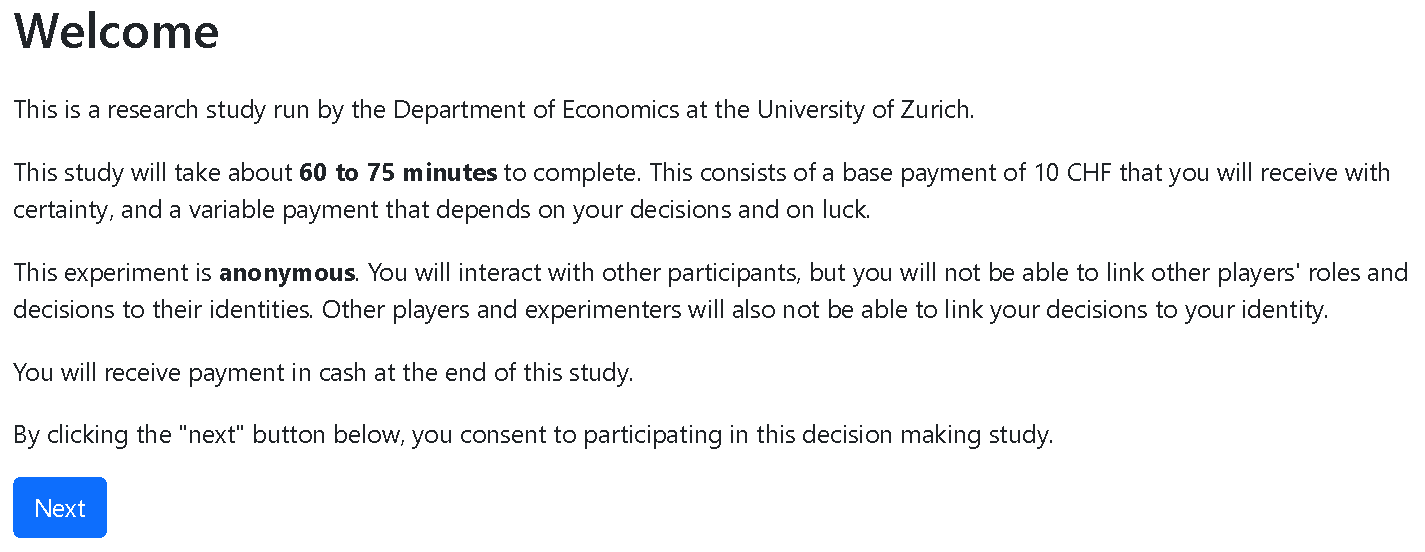
\includegraphics[width=.9\linewidth]{screenshots/welcome.pdf}
    \caption{Welcome screen}
\end{figure}

\begin{figure}[!htb]
    \centering
    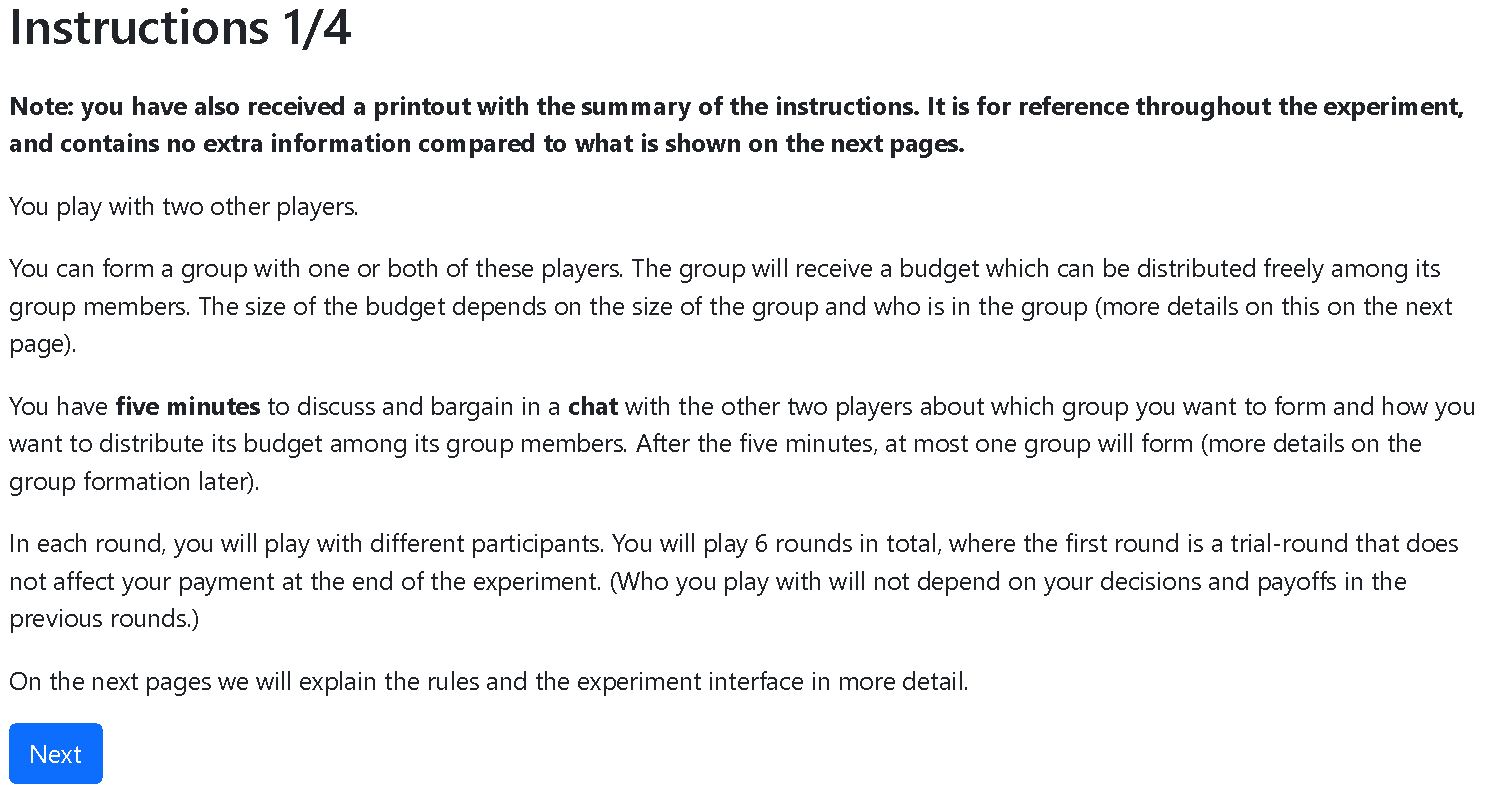
\includegraphics[width=.9\linewidth]{screenshots/instructions_1.pdf}
    \caption{Instructions 1/4: Introduction}
\end{figure}

\begin{figure}[!htb]
    \centering
    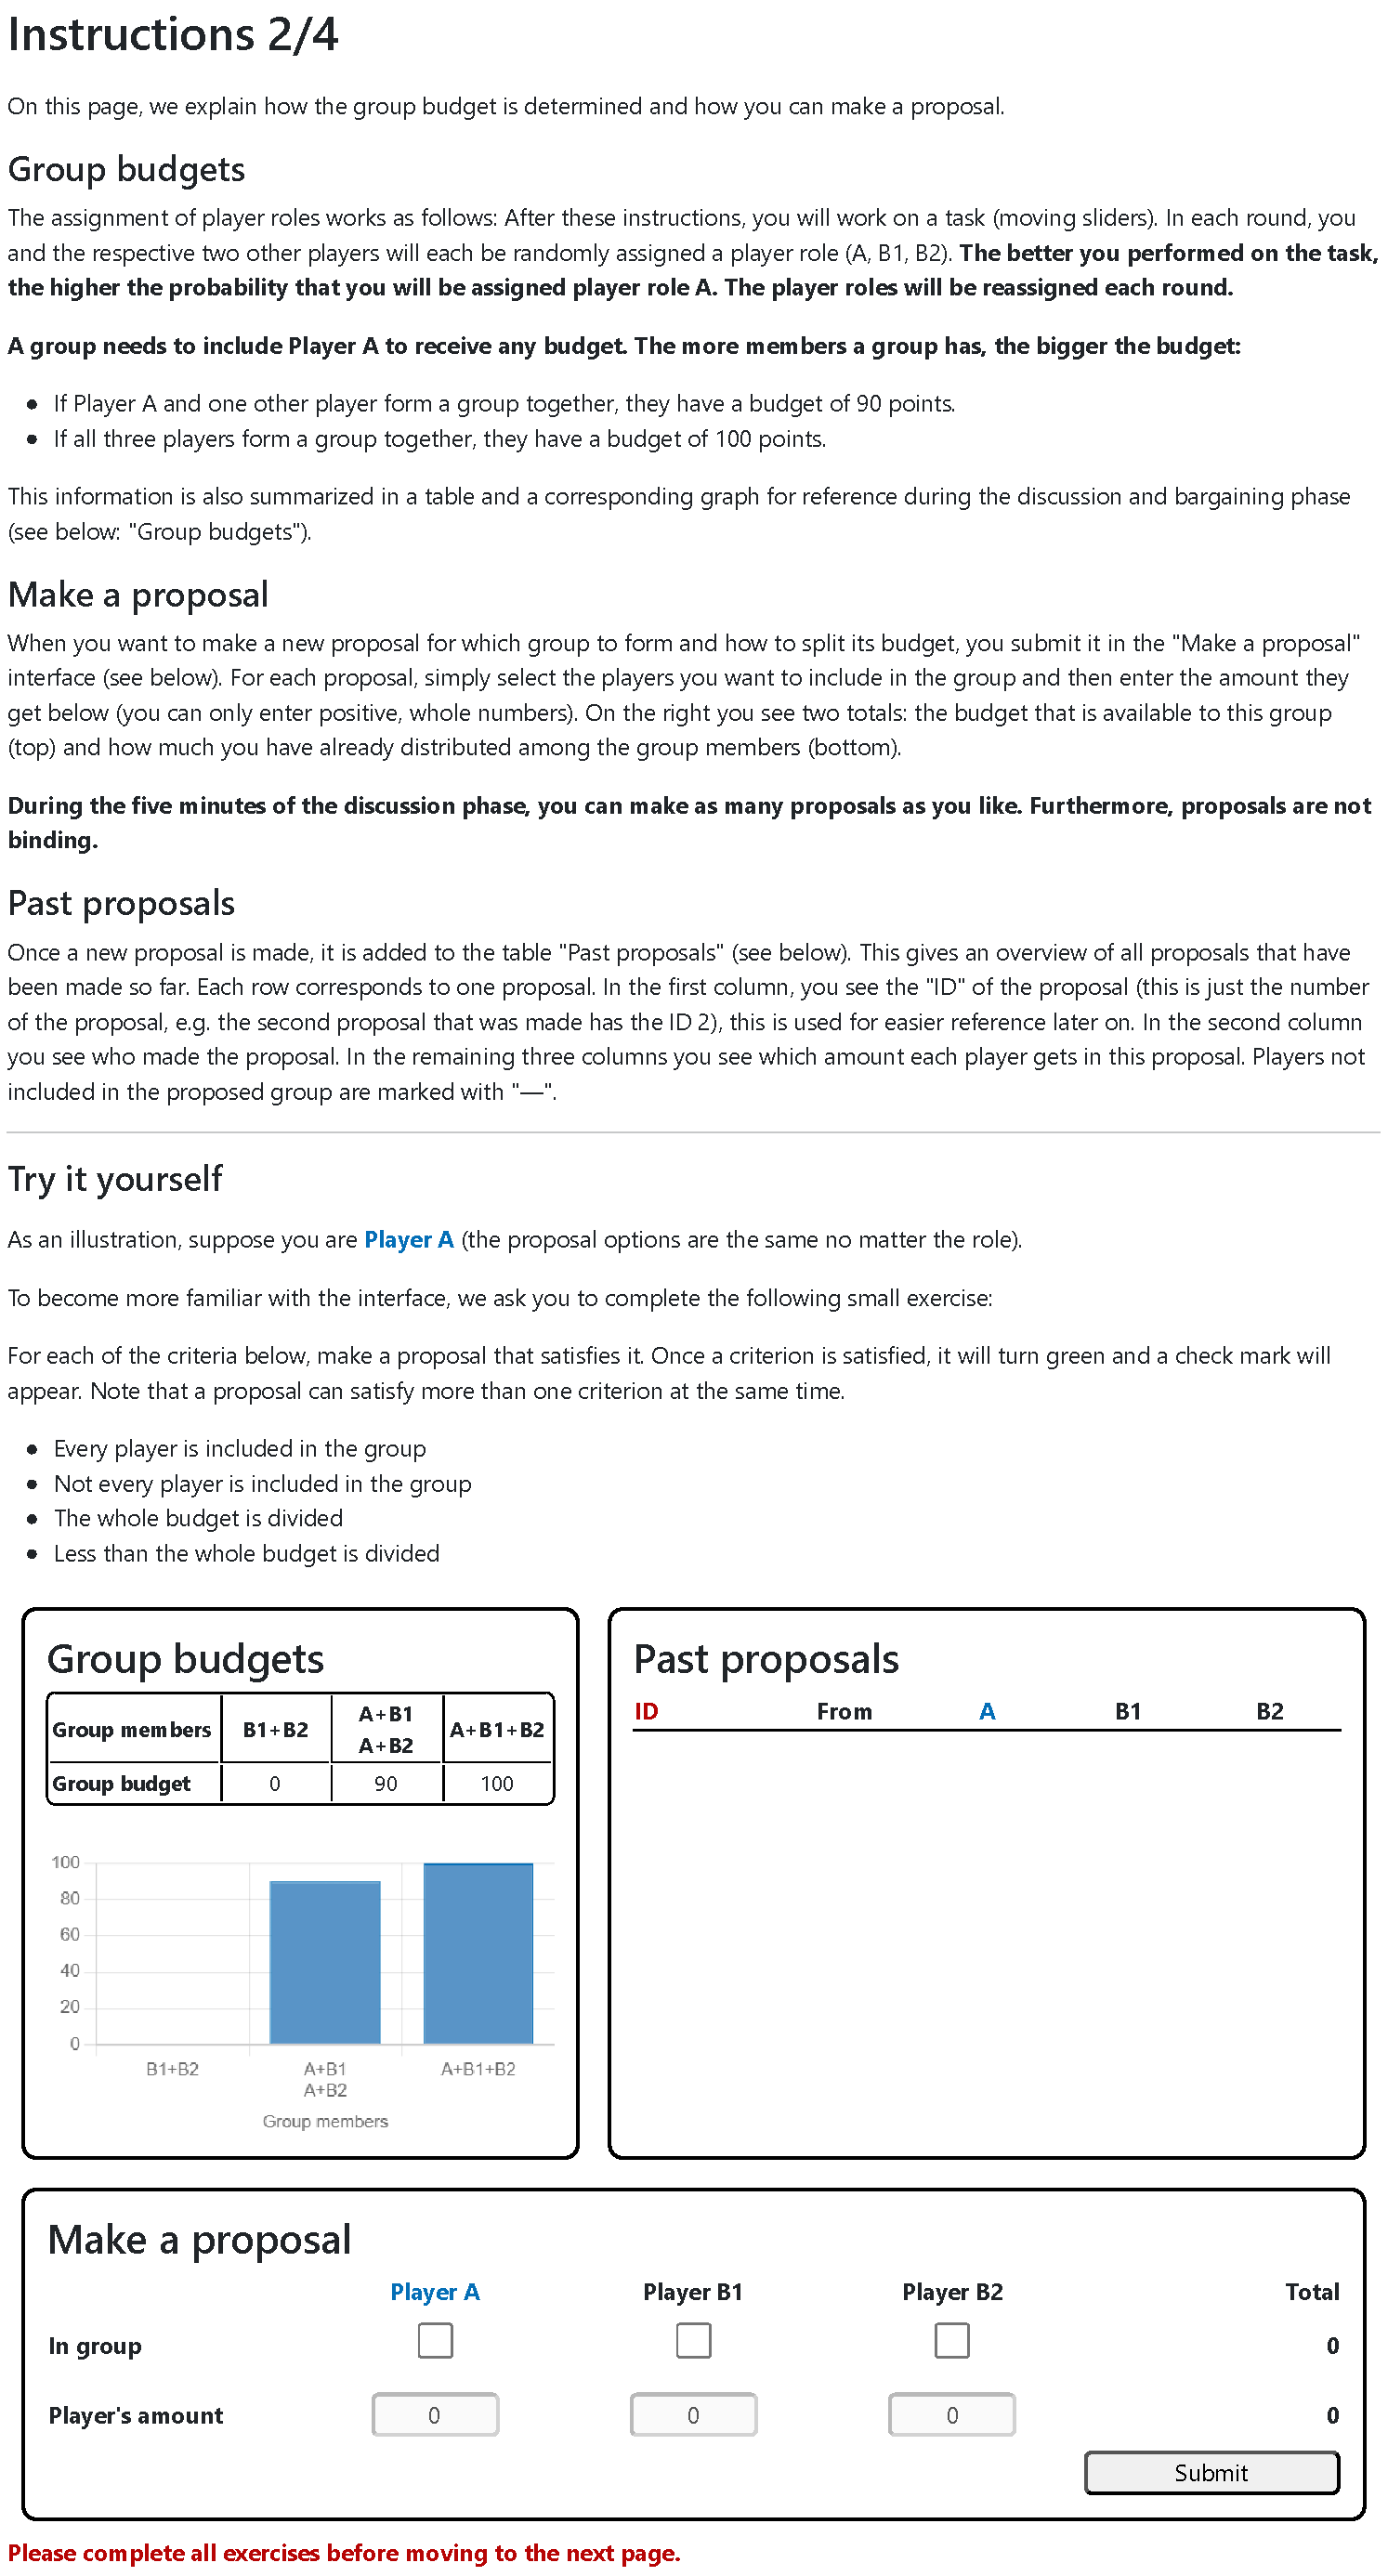
\includegraphics[width=.7\linewidth]{screenshots/instructions_2.pdf}
    \caption{Instructions 2/4: Group budgets}
\end{figure}


\begin{figure}[!htb]
    \centering
    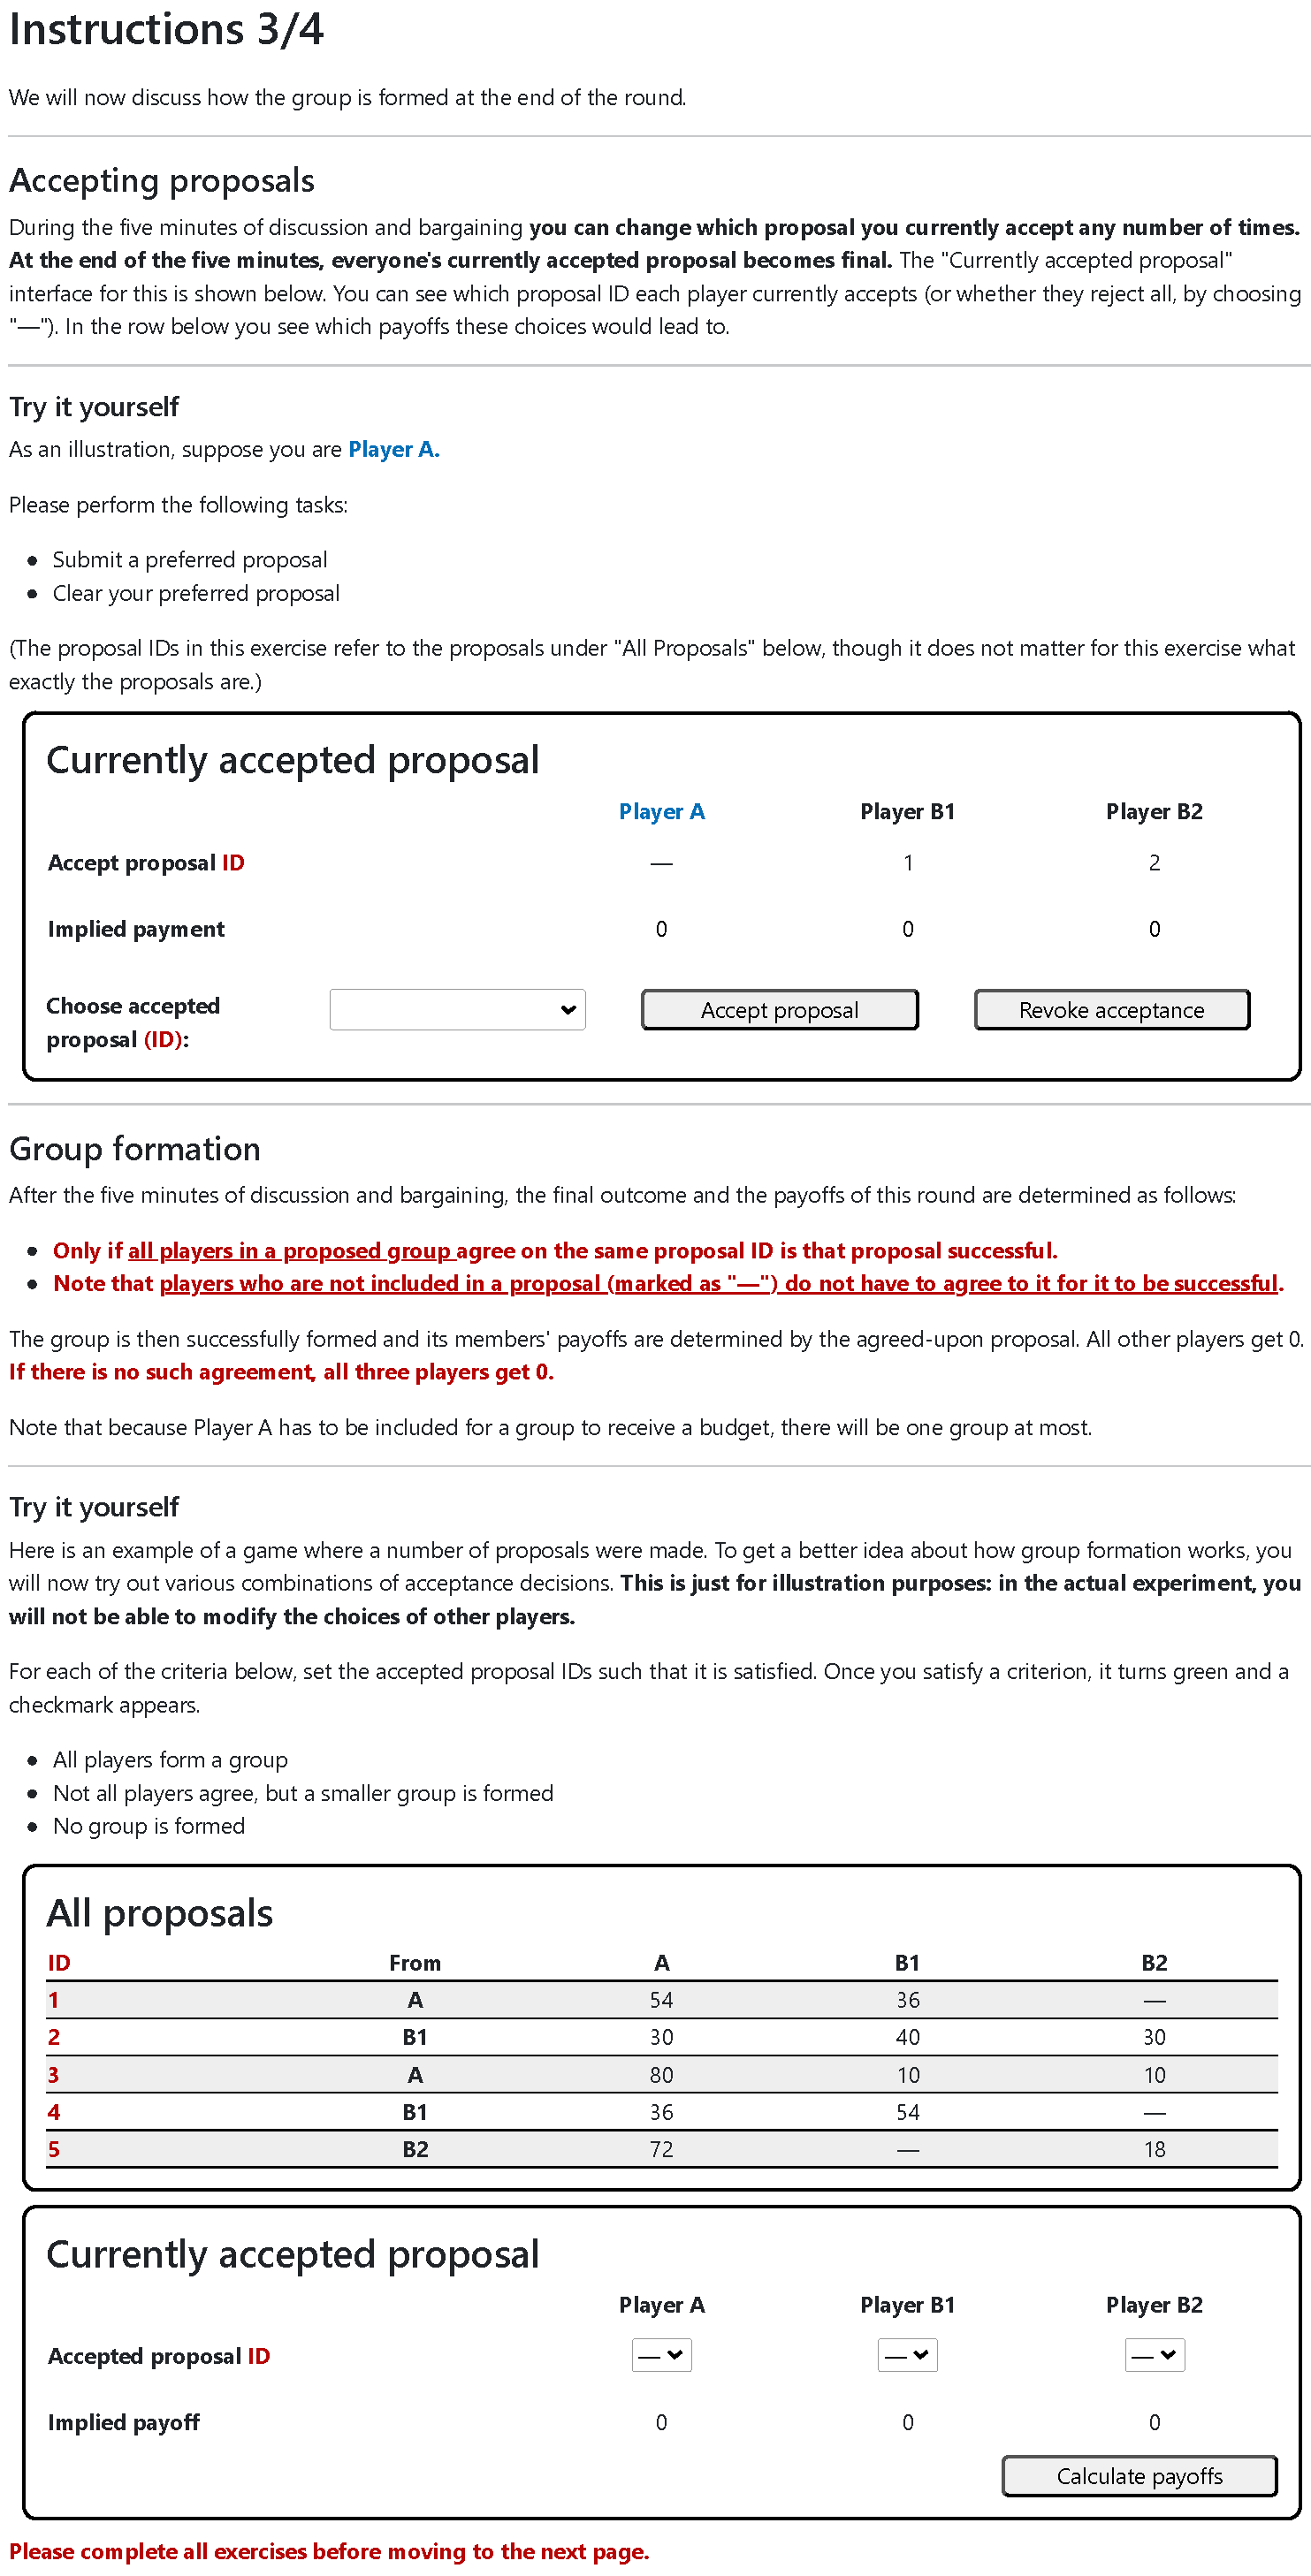
\includegraphics[width=.7\linewidth]{screenshots/instructions_3.pdf}
    \caption{Instructions 3/4: Proposals and group formation}
\end{figure}

\begin{figure}[!htb]
    \centering
    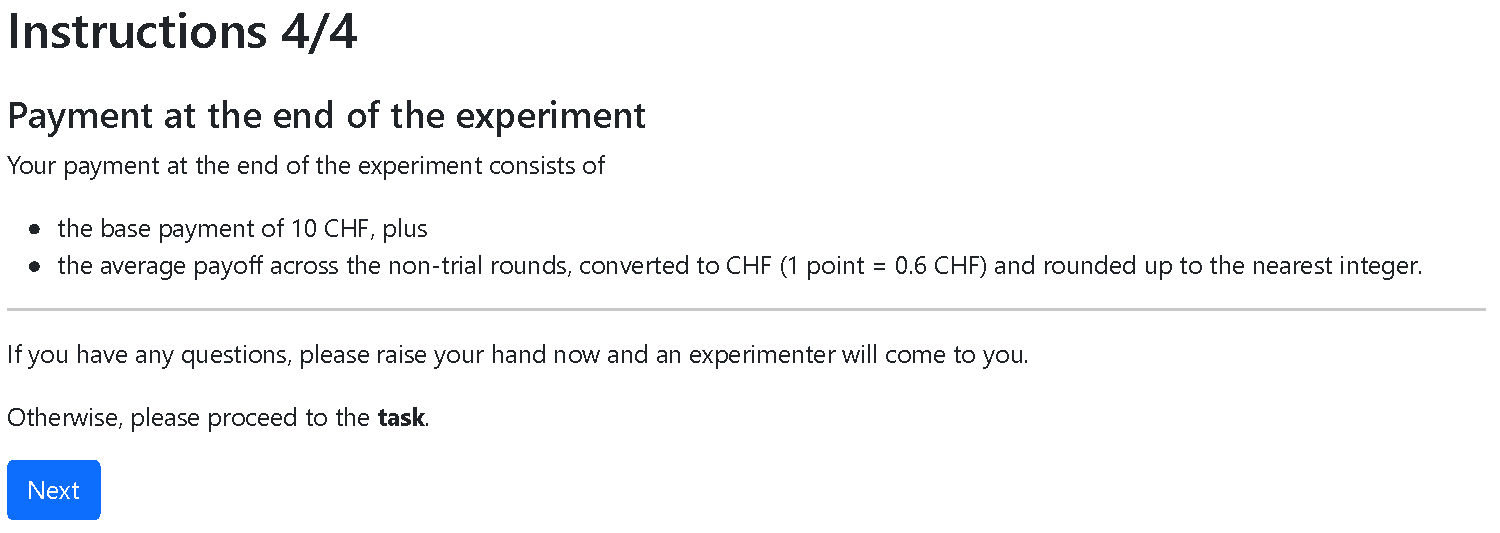
\includegraphics[width=.9\linewidth]{screenshots/instructions_4.pdf}
    \caption{Instructions 4/4: Payment}
\end{figure}


\begin{figure}[!htb]
   \begin{subfigure}[b]{\textwidth}
        \centering
        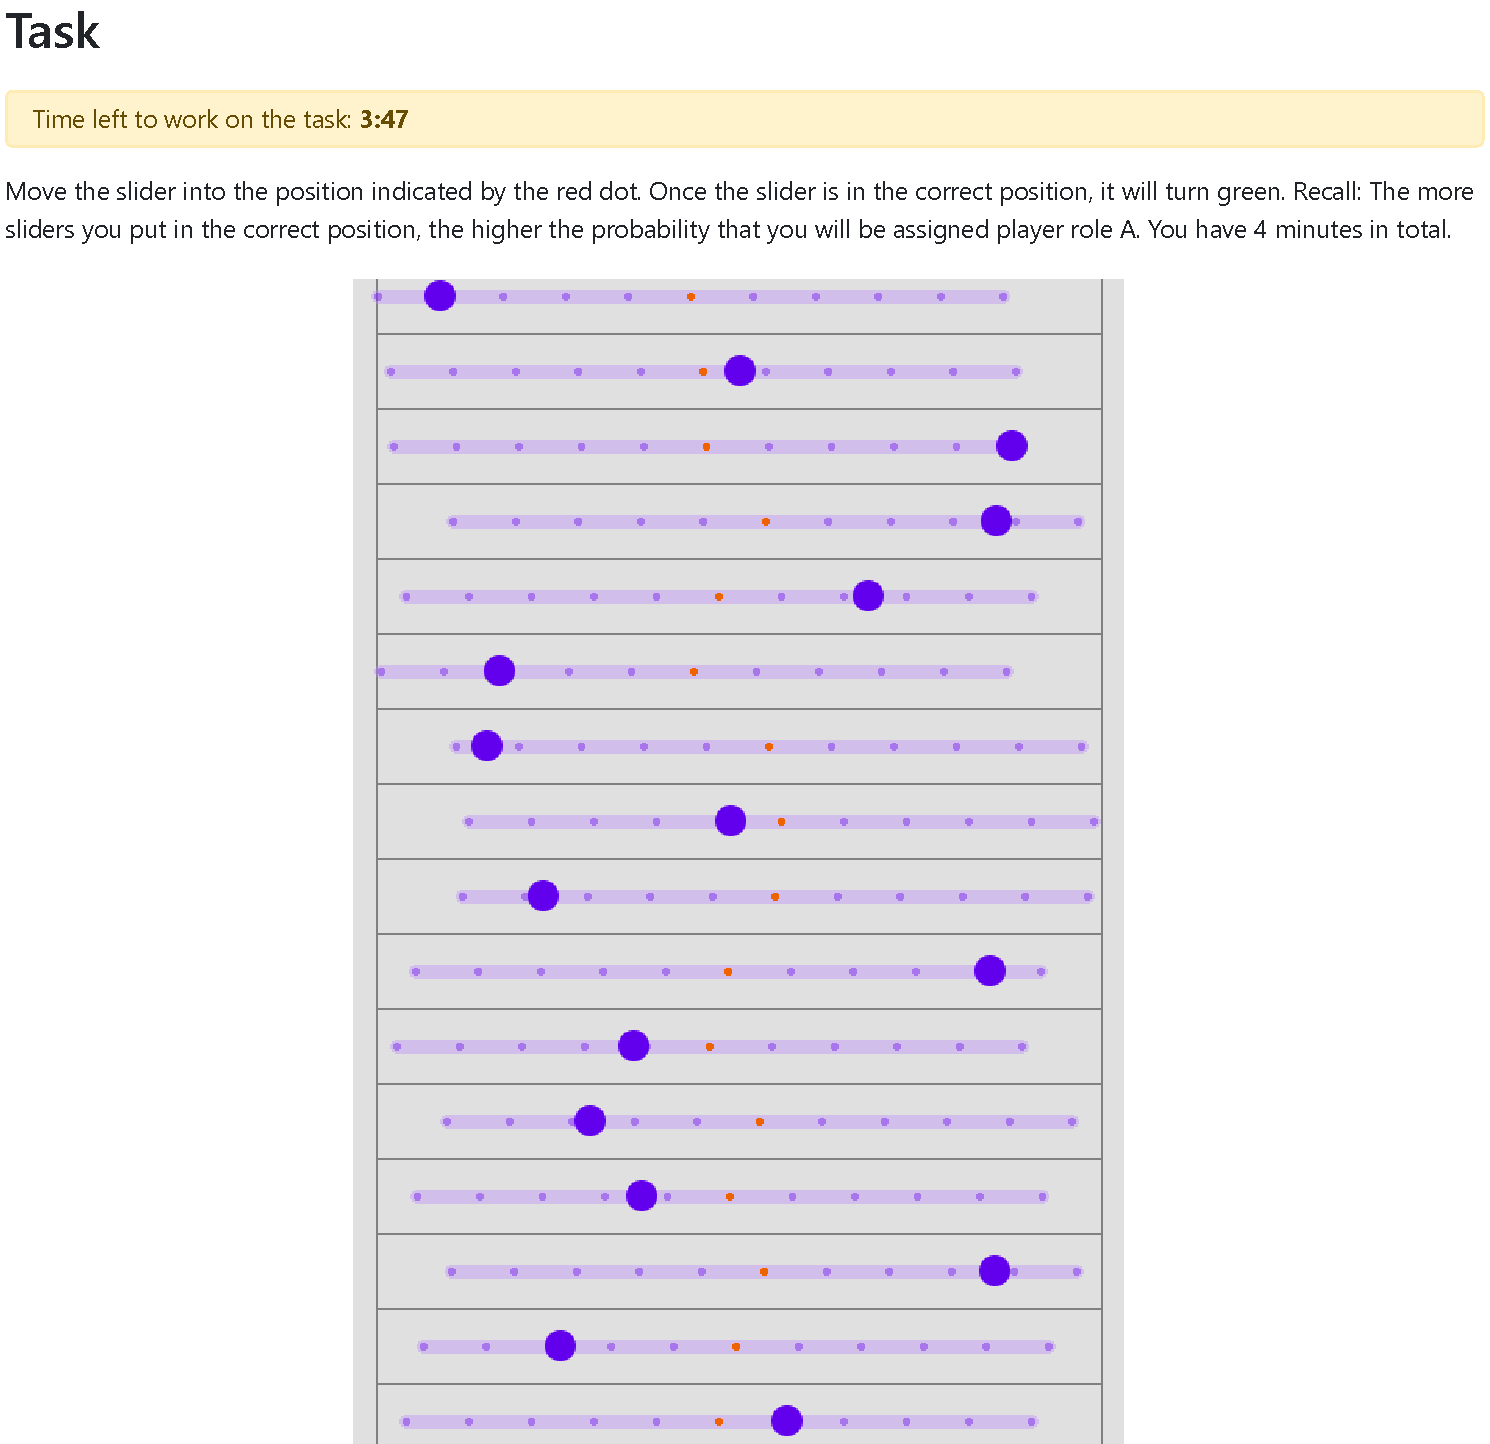
\includegraphics[width=0.9\textwidth]{screenshots/slider.pdf}
    \end{subfigure}
    \par\bigskip
    \begin{subfigure}[b]{\textwidth}
        \centering
        
\includegraphics[width=0.5\textwidth]{screenshots/slider_results.pdf}
    \end{subfigure}
    \caption{Slider task. (Note that this screenshot is cropped, there were 150 sliders in total.)}
\end{figure}

\begin{figure}[!htb]
    \centering
    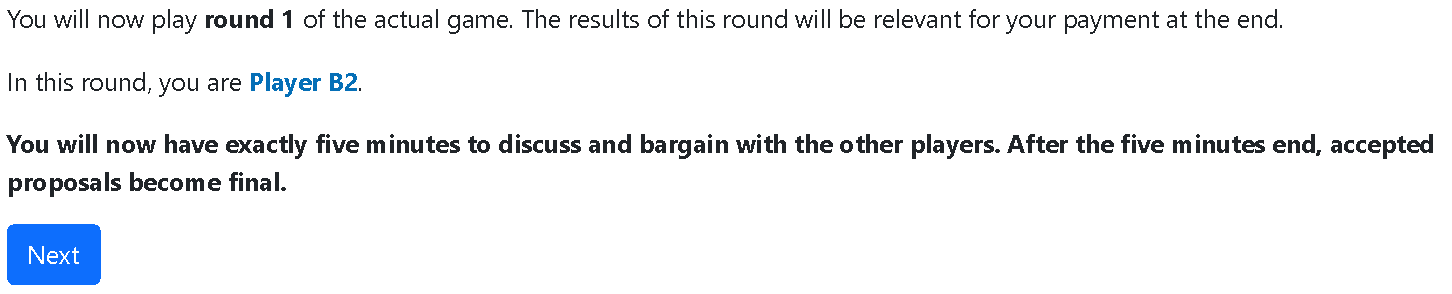
\includegraphics[width=.9\linewidth]{screenshots/info.pdf}
    \caption{Info page before the bargaining round}
\end{figure}

\begin{figure}[!htb]
    \centering
    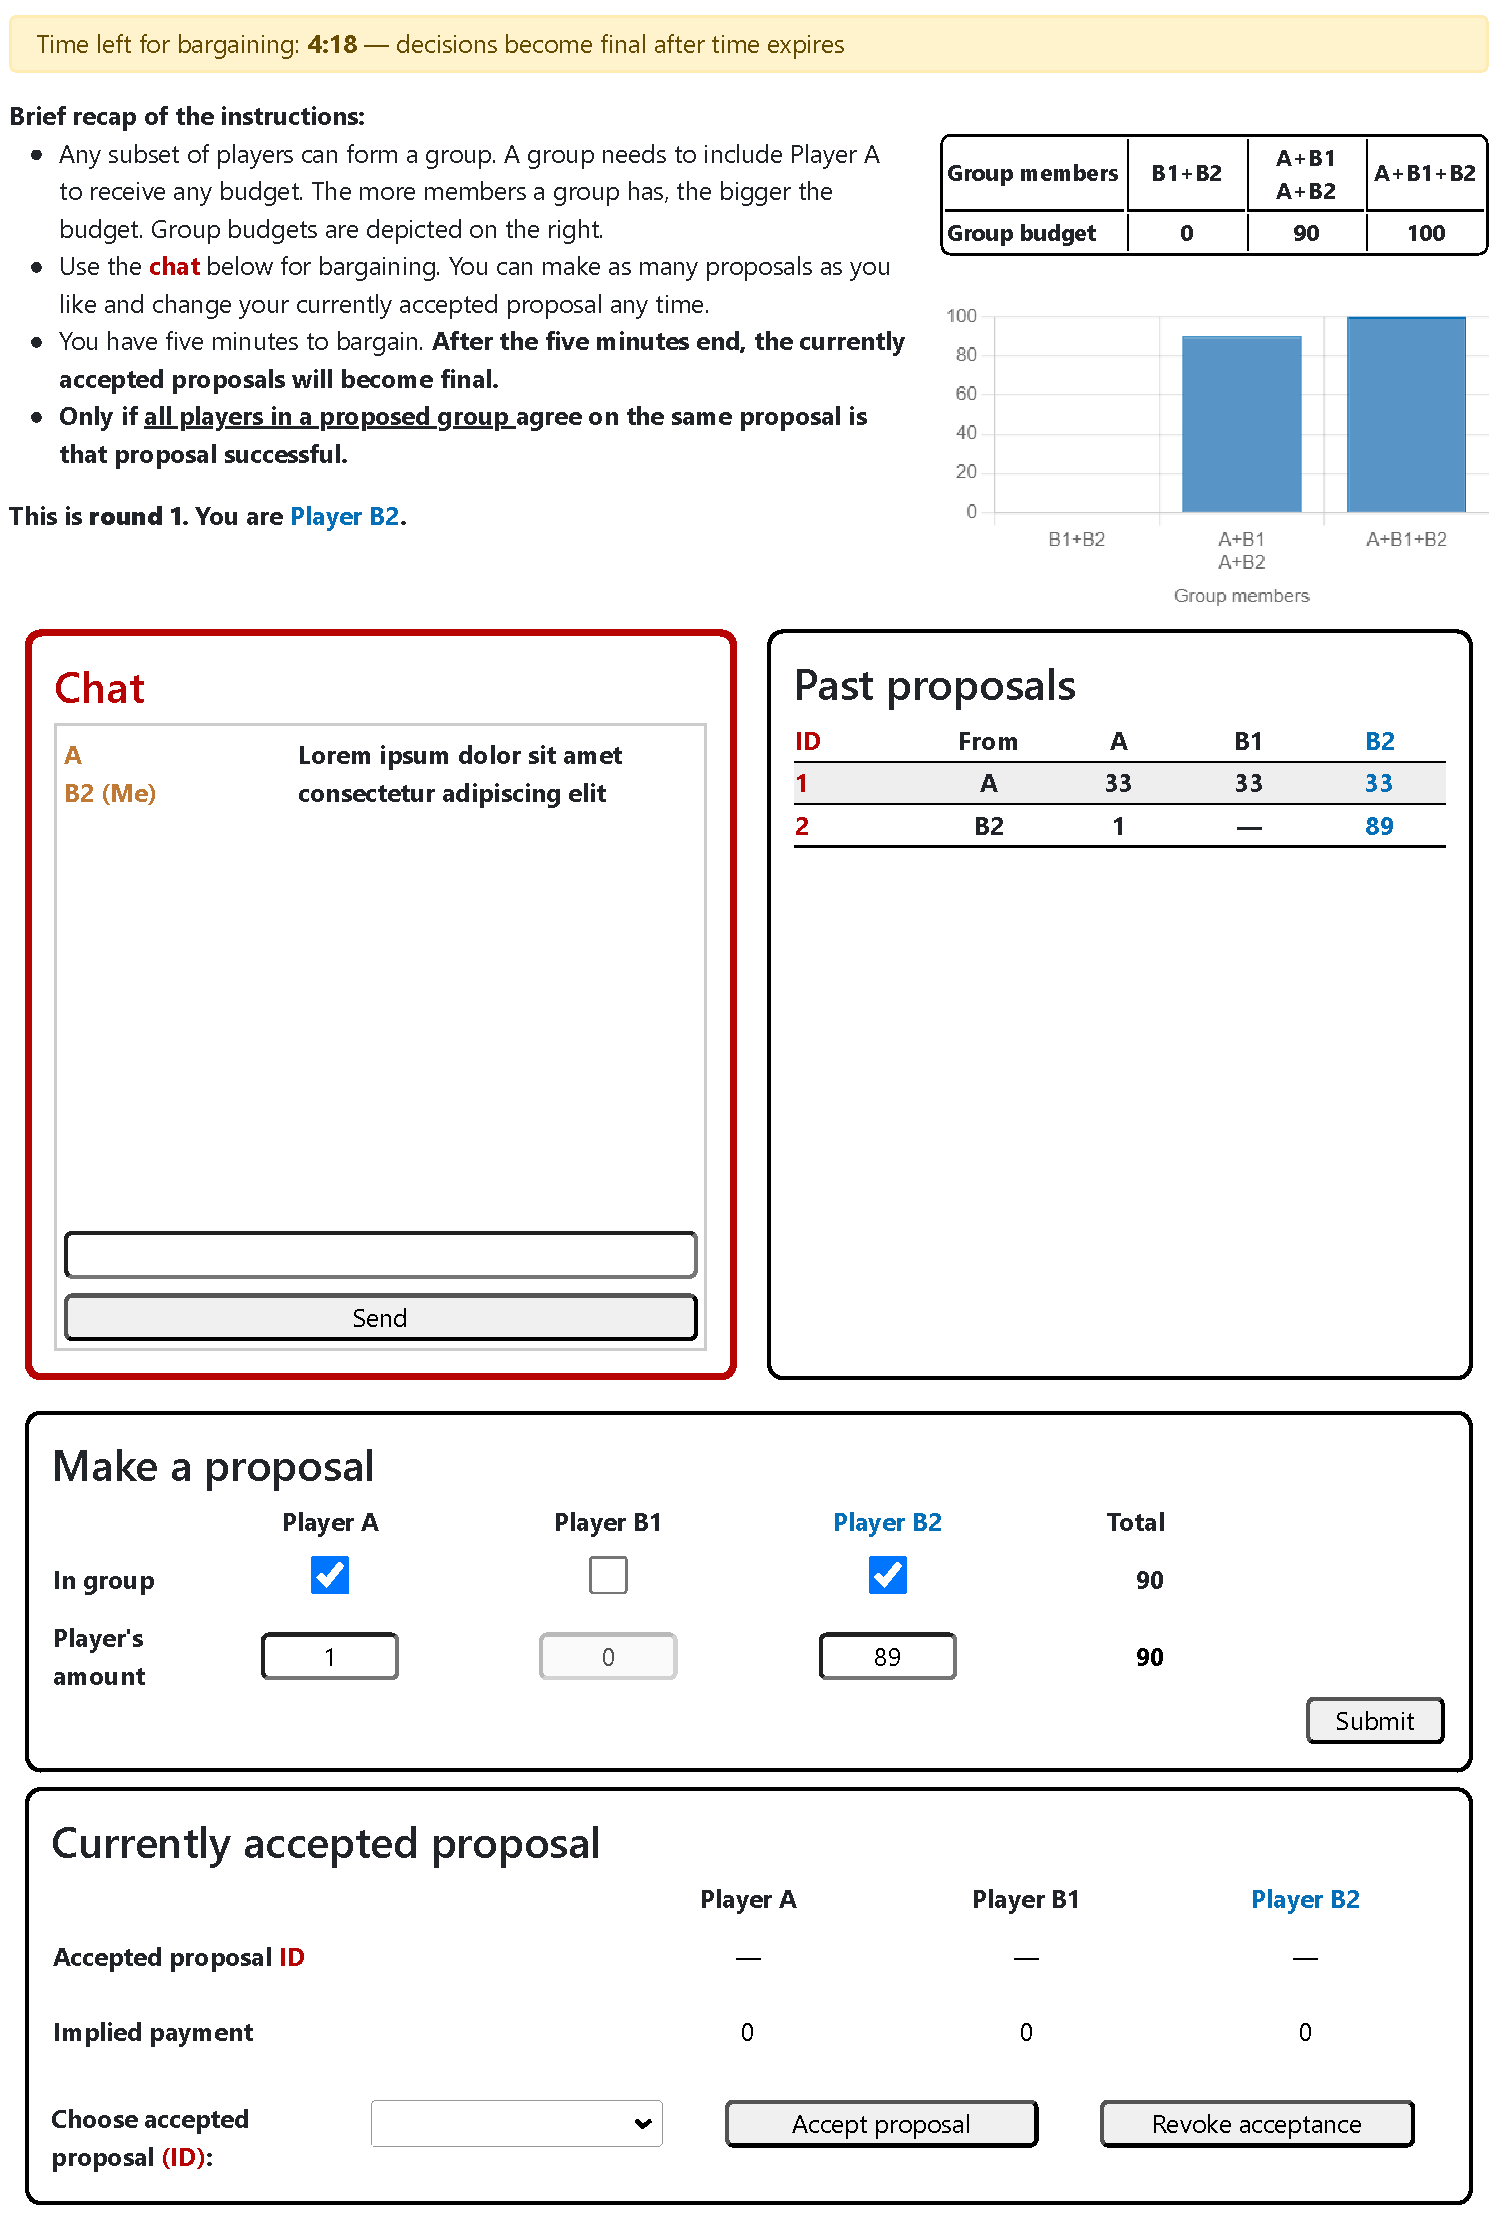
\includegraphics[width=.8\linewidth]{screenshots/bargaining_interface.pdf}
    \caption{Bargaining interface}
    \label{bargaining_interface}
\end{figure}


\section{Chat analysis}

\subsection{Methodology}
\label{sec:gpt_prompt}

To ensure reproducibility as much as possible, the temperature of the GPT-4o model was set to zero. The system prompt we supplied was the following:
\begin{lstlisting}[captionpos=b,caption=System prompt for GPT-4o]
You are going to receive a log containing messages between three players from an economics lab experiment. Players bargained how to split an amount of money. They could additionally use an interface for submitting and accepting proposals. Before the bargaining, players did a slider task and their performance determined their bargaining position.

The log format is the following:
MSG #[MESSAGE_ID] @[PLAYER_NAME]: [MESSAGE]
PROP #[PROPOSAL_ID] @[PLAYER_NAME]: [distribution of the money]
ACC #[ACCEPTANCE_ID] @[PLAYER_NAME]: PROP #[PROPOSAL_ID]
separated by newlines.

Please classify which TOPIC each message (MSG) belongs to. You only have to classify messages, not proposals or acceptances (those latter two are only included for context). The classification should also take into account the context of the message (e.g. when a message is a reply to another).
Each message should be classified into one main and one subtopic. The topics are given in the following nested list:
 - small talk: messages that are not directly related to the experiment
    - greetings and farewells: e.g. saying hello, goodbye, etc.
    - other: e.g. talking about the weather, how to spend the remaining time, etc.
 - bargaining: messages discussing the distribution of the money, making and reacting to proposals, counter-proposals, etc.
    - fairness-based: using arguments based on fairness or justice ideas
    - non-fairness-based: using arguments based on other considerations
 - meta-talk: talking about the experiment itself
    - purpose: discussing what the experimenters are trying to find out
    - rules: discussing and clarifying the rules of the experiment
    - identification: identifying each other, e.g. trying to figure out if players met each other in previous rounds, or identifying information for later

Your response should be of the following format:
#[MESSAGE_ID]: [MAIN_TOPIC], [SUB_TOPIC]
for each message, separated by newlines.
It should look like the contents of a dictionary, but without the surrounding curly braces and apostrophes.
Do not include any other lines, such as code block delimiters or comments.
If there are no rows of type MSG, please respond with NO_MESSAGES without any additional content, such as IDs or comments.
\end{lstlisting}

Then, we supplied the chat, proposal and acceptance history for a given round as the user prompt. An example is given below.
\begin{lstlisting}[captionpos=b,caption=User prompt for GPT-4o]
MSG #1 @A: what are you guys up to?
PROP #1 @B2: A: 34, B1: 33, B2: 33
MSG #2 @A: anyone one split 90 points with me?
MSG #3 @B2: fair play
MSG #4 @B2: propose A
PROP #2 @A: A: 45, B1: 0, B2: 45
ACC #1 @A: PROP #2
MSG #5 @B2: fair i'm down
ACC #2 @B2: PROP #2
MSG #6 @A: i mean if B1 has nothing to say
MSG #7 @A: feel free to offer a better deal :)
MSG #8 @B1: I will not accept it, but i do not think it matters at this point xd
ACC #3 @B1: PROP #0
MSG #9 @A: nope only thing you can do is propose a better deal for me hahah
MSG #10 @A: sorry m8
PROP #3 @B1: A: 46, B1: 44, B2: 0
MSG #11 @A: the power of A
MSG #12 @B1: xdxd no problem
ACC #4 @A: PROP #3
ACC #5 @B1: PROP #3
MSG #13 @A: xD
MSG #14 @A: lets get that game rolling
MSG #15 @A: im sure B2 cannot be happy with that
MSG #16 @B1: hahaha
MSG #17 @B2: :) just wait and see
MSG #18 @A: deal before 10 sek
PROP #4 @B2: A: 50, B1: 0, B2: 40
ACC #6 @B2: PROP #4
ACC #7 @A: PROP #4
\end{lstlisting}

Finally, the model's answer was as follows.
\begin{lstlisting}[captionpos=b,caption=Answer from GPT-4o]
#1: small talk, other
#2: bargaining, non-fairness-based
#3: bargaining, fairness-based
#4: bargaining, non-fairness-based
#5: bargaining, fairness-based
#6: bargaining, non-fairness-based
#7: bargaining, non-fairness-based
#8: bargaining, non-fairness-based
#9: bargaining, non-fairness-based
#10: small talk, other
#11: small talk, other
#12: small talk, other
#13: small talk, other
#14: small talk, other
#15: bargaining, non-fairness-based
#16: small talk, other
#17: small talk, other
#18: bargaining, non-fairness-based
\end{lstlisting}

The results of the categorization of messages is included in the project's git repository along with the raw data.

\subsection{Chat excerpts}
\label{sec:chat_excerpts}

This section contains a number of chat excerpts (including proposals and acceptance decisions) to illustrate some more common themes we observed when reviewing the chat logs. They are presented mostly to give an idea about the kind of textual data we obtained from the experiment.

\begin{figure}[!htb]
    \centering
    \begin{subfigure}[b]{0.42\textwidth}
        \centering
        \includegraphics[width=\linewidth]{out/figures/chat_excerpt-5640,5647-5648,5660-5663.pdf}
        \caption{Treatment $Y=30$: discussing that partial agreement makes no sense}
        \label{fig:chat_stability_y30}
    \end{subfigure}
    \hspace{0.1\textwidth}
    \begin{subfigure}[b]{0.42\textwidth}
        \centering
        \includegraphics[width=\linewidth]{out/figures/chat_excerpt-6846-6847,6849,6851,6853,6855,6857,6859.pdf}
        \caption{Treatment $Y=90$: making the small players compete}
        \label{fig:chat_stability_y90}
    \end{subfigure}
    \caption{Examples of stability-based reasoning from the chat logs. Note, that some messages have been omitted.}
    \label{fig:chat_stability}
\end{figure}

\begin{figure}[!htb]
    \centering
    \begin{subfigure}[b]{0.42\textwidth}
        \centering
        \includegraphics[width=\linewidth]{out/figures/chat_excerpt-7052,7054,7057-7063.pdf}
        \caption{Treatment $Y=90$:, agreeing on almost equal split}
        \label{fig:chat_fairness_equal_split}
    \end{subfigure}
    \hspace{0.1\textwidth}
    \begin{subfigure}[b]{0.42\textwidth}
        \centering
        \includegraphics[width=\linewidth]{out/figures/chat_excerpt-7894-7901,7906.pdf}
        \caption{Treatment $Y=90$: rejecting unequal proposals}
        \label{fig:chat_fairness_reject_small}
    \end{subfigure}
    \caption{Examples of fairness-based reasoning from the chat logs. Note that some messages have been omitted for brevity.}
    \label{fig:chat_fairness}
\end{figure}

\begin{figure}[!htb]
    \centering
    \begin{subfigure}[b]{0.42\textwidth}
        \centering
        \includegraphics[width=\linewidth]{out/figures/chat_excerpt-6508-6509,6511,6513,6524,6527,6528-6529.pdf}
        \caption{Discussing the impact of having the ability to chat with each other}
        \label{fig:chat_meta_chat}
    \end{subfigure}
    \hspace{0.1\textwidth}
    \begin{subfigure}[b]{0.42\textwidth}
        \centering
        \includegraphics[width=\linewidth]{out/figures/chat_excerpt-5501-5508.pdf}
        \caption{Small talk and feedback about the length of the rounds}
        \label{fig:chat_meta_time}
    \end{subfigure}
    \caption{Examples of discussing the experiment from the chat logs. Note that some messages have been omitted for brevity.}
    \label{fig:chat_meta}
\end{figure}

\section{Payoffs by matching group}

\begin{figure}[!htb]
    \centering
    \includegraphics[width=1\linewidth]{out/figures/payoff_matching_group_average_rounds_all.pdf}
    \caption{Average payoff on the matching-group level by role and treatment. (There were six matching groups à six subjects in each treatment.)}
    \label{fig:matching_group}
\end{figure}

\section{Reciprocity concerns}

\begin{figure}[!htb]
    \centering
    \begin{subfigure}[b]{0.49\textwidth}
        \centering
        \includegraphics[width=\textwidth]{out/figures/payoff_average_rounds_[2,3,4,5].pdf}
        \caption{Rounds 1-4}
    \end{subfigure}
    \hfill
    \begin{subfigure}[b]{0.49\textwidth}
        \centering
        \includegraphics[width=\textwidth]{out/figures/payoff_average_rounds_[6].pdf}
        \caption{Round 5}
    \end{subfigure}
    \caption{Average payoffs for each player role by treatment, for the given rounds. Vertical bars denote 95\% confidence intervals for the within-group means.}
    \label{fig:reciprocity}
\end{figure}

A potential concern is that reciprocity is a driver of behavior and leads to more equal payoffs: for example, people might give a non-zero payoff to the dummy player because they expect to be the dummy player in later rounds, or they might agree on outcomes closer to the equal split because they expect to be a small player in later rounds. This is corroborated by the fact that some subjects try to identify each other (\Cref{fig:chat_topics_all}). While a large part of it is due to small talk about topics such as countries of origin or degrees, some subjects tried to agree on code words in order to identify each in later rounds, for example in order to find out if groups were actually reshuffled. Reciprocity, however, would suggest that the behavior in the last round is different from the previous rounds. While we can not exclude that reciprocity is a factor, the comparison of the average payoffs of the last rounds versus all other non-trial rounds does not indicate any substantial difference.

\section{Survey: axioms}

\begin{figure}[!htb]
    \centering
    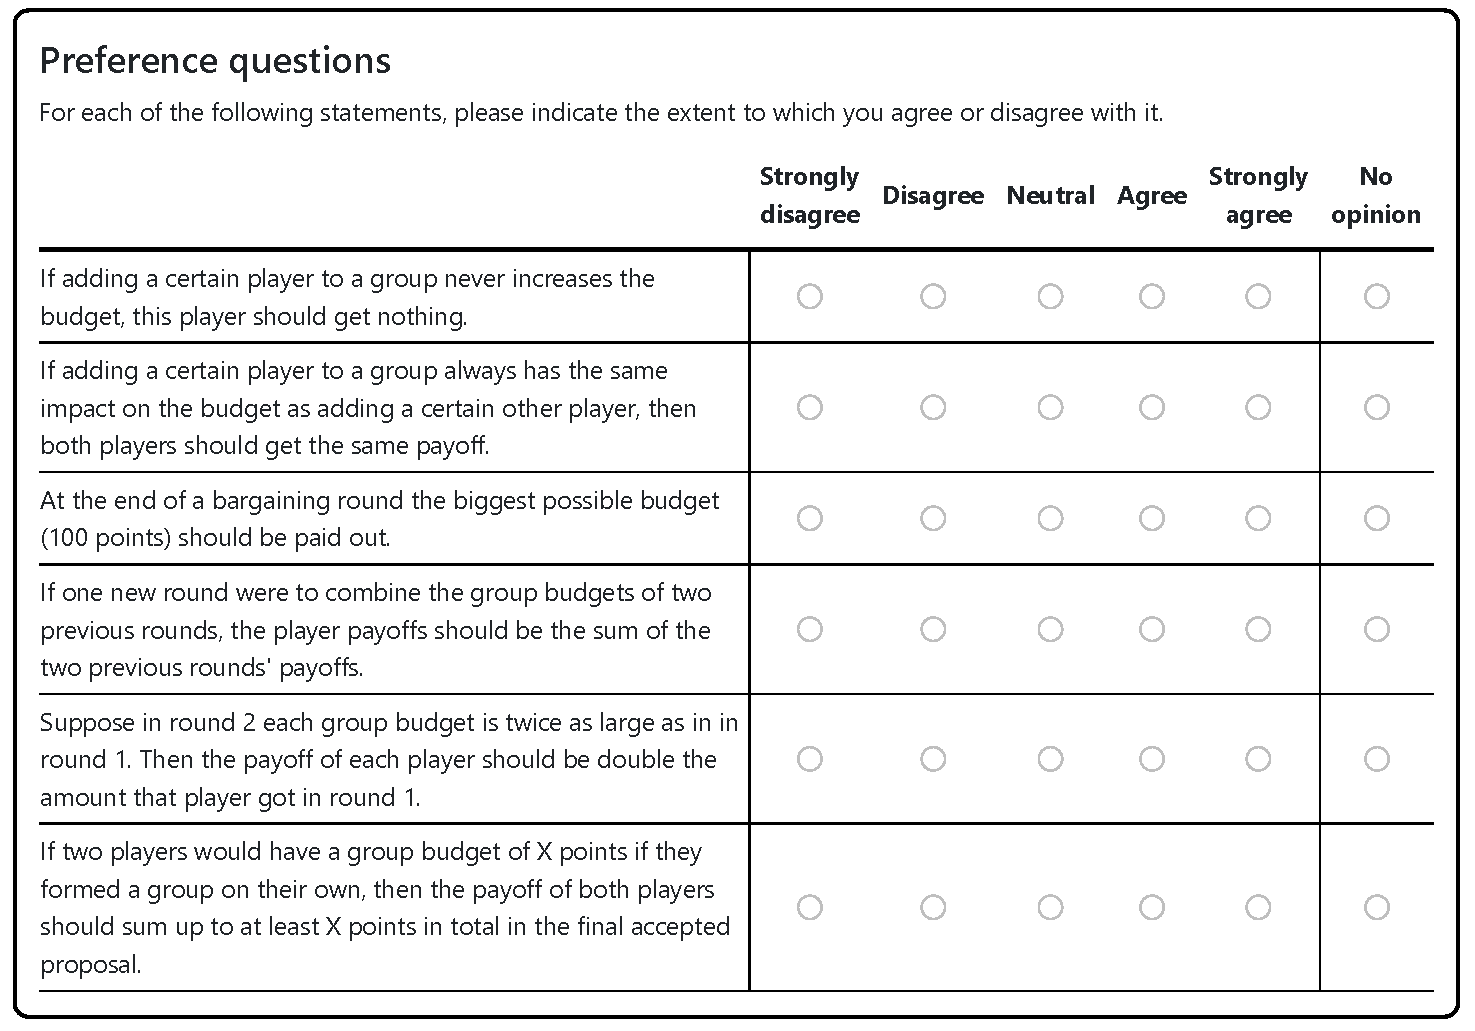
\includegraphics[width=.9\linewidth]{screenshots/survey_axioms.pdf}
    \caption{Survey questions for the axioms}
    \label{fig:survey_axioms_questions}
\end{figure}



\begin{figure}
    \centering
    \includegraphics[width=.99\linewidth]{out/figures/axioms_survey_efficiency.pdf}
    \includegraphics[width=.99\linewidth]{out/figures/axioms_survey_symmetry.pdf}
    \includegraphics[width=.99\linewidth]{out/figures/axioms_survey_linearity_additivity.pdf}
    \includegraphics[width=.99\linewidth]{out/figures/axioms_survey_linearity_HD1.pdf}
    \caption{Survey: empirical support of the axioms}
    \label{fig:axioms_survey_1}
\end{figure}

\begin{figure}
    \ContinuedFloat
    \centering
    \includegraphics[width=.99\linewidth]{out/figures/axioms_survey_dummy_player.pdf}
    \includegraphics[width=.99\linewidth]{out/figures/axioms_survey_stability.pdf}
    \caption{Survey: empirical support of the axioms}
    \label{fig:axioms_survey_2}
\end{figure}


\begin{figure}
    \centering
    \includegraphics[width=1\linewidth]{out/figures/allocations_proposals_by_dummy_player_axiom.pdf}
    \caption{Proposals by agreement with the dummy player axiom.}
    \label{fig:axioms_proposals_dummy_player}
\end{figure}

\begin{figure}
    \centering
    \includegraphics[width=1\linewidth]{out/figures/allocations_proposals_by_symmetry_axiom.pdf}
    \caption{Proposals by agreement with the symmetry axiom.}
    \label{fig:axioms_proposals_symmetry}
\end{figure}

\begin{figure}
    \centering
    \includegraphics[width=1\linewidth]{out/figures/allocations_proposals_by_efficiency_axiom.pdf}
    \caption{Proposals by agreement with the efficiency axiom.}
    \label{fig:axioms_proposals_efficiency}
\end{figure}

\begin{figure}
    \centering
    \includegraphics[width=1\linewidth]{out/figures/allocations_proposals_by_linearity_HD1_axiom.pdf}
    \caption{Proposals by agreement with the linearity (homogeneity of degree 1) axiom.}
    \label{fig:axioms_proposals_linearity_HD1}
\end{figure}

\begin{figure}
    \centering
    \includegraphics[width=1\linewidth]{out/figures/allocations_proposals_by_linearity_additivity_axiom.pdf}
    \caption{Proposals by agreement with the linearity (additivity) axiom.}
    \label{fig:axioms_proposals_linearity_additivity}
\end{figure}

\begin{figure}
    \centering
    \includegraphics[width=1\linewidth]{out/figures/allocations_proposals_by_stability_axiom.pdf}
    \caption{Proposals by agreement with the stability axiom.}
    \label{fig:axioms_proposals_stability}
\end{figure}

\section{Subject sample: Population characteristics} 

\begin{figure}[!h]
    %\centering
    \begin{subfigure}[b]{0.49\textwidth}
        \centering
        \includegraphics[width=\textwidth]{out/figures/survey_gender.pdf}
        \caption{Gender composition, by treatment.}
        \label{fig:balance_gender}
    \end{subfigure}
    \hfill
    \begin{subfigure}[b]{0.49\textwidth}
        \centering
        \includegraphics[width=\textwidth]{out/figures/survey_degree.pdf}
        \caption{Degree composition, by treatment.}
        \label{fig:balance_degree}
    \end{subfigure}
    \vfill
    \begin{subfigure}[b]{0.43\textwidth}
         \centering
        \includegraphics[width=\textwidth]{out/figures/survey_age.pdf}
        \caption{Average age, by treatment.}
        \label{fig:balance_age}
    \end{subfigure}
    \label{fig:balance}
\end{figure}

\begin{figure}
    \ContinuedFloat
    \centering
    \begin{subfigure}[b]{\textwidth}
        \centering
        \includegraphics[width=1\textwidth]{out/figures/survey_nationality.pdf}
        \caption{Nationality composition, by treatment.}
        \label{fig:survey_nationality}
    \end{subfigure}
    \caption{Population characteristics of the experiment sample, by treatment.}
    \label{fig:balance_cont}
\end{figure}

\end{subappendices}

\singlespacing

\addcontentsline{toc}{chapter}{Bibliography}
\printbibliography

\end{document}
